\documentclass{article}

\usepackage{graphicx}
\usepackage{amsmath}
\usepackage{mathtools}
\usepackage{lmodern}
\usepackage{natbib}
\usepackage[figuresright]{rotating}
\usepackage{amsmath,amssymb}
\usepackage{bbm}
\usepackage{enumerate}
\usepackage{graphicx}
\usepackage{subcaption}
\captionsetup{compatibility=false}
\font\myfont=cmr12 at 15pt
\renewcommand{\baselinestretch}{1.0}
\setlength{\baselineskip}{20pt}
\usepackage{amssymb,amsmath}
\usepackage{ifxetex,ifluatex}
\linespread{1.6} 
\ifnum 0\ifxetex 1\fi\ifluatex 1\fi=0 % if pdftex
  \usepackage[T1]{fontenc}
\else 
  \ifxetex
    \usepackage{mathspec}
  \else
    \usepackage{fontspec}
  \fi
  \defaultfontfeatures{Ligatures=TeX,Scale=MatchLowercase}
\fi
\IfFileExists{upquote.sty}{\usepackage{upquote}}{} \IfFileExists{microtype.sty}{
\usepackage{microtype}
\UseMicrotypeSet[protrusion]{basicmath}}{}
\usepackage[margin=1in]{geometry}
\usepackage{hyperref}
\urlstyle{same}  % don't use monospace font for urls
\usepackage{graphicx,grffile}
\makeatletter
\def\maxwidth{\ifdim\Gin@nat@width>\linewidth\linewidth\else\Gin@nat@width\fi}
\def\maxheight{\ifdim\Gin@nat@height>\textheight\textheight\else\Gin@nat@height\fi}
\makeatother

\setkeys{Gin}{width=\maxwidth,height=\maxheight,keepaspectratio}
\IfFileExists{parskip.sty}{%
\usepackage{parskip}
}{
\setlength{\parindent}{0pt}
\setlength{\parskip}{6pt plus 2pt minus 1pt}
} \setlength{\emergencystretch}{3em}  % prevent overfull lines
\providecommand{\tightlist}{%
  \setlength{\itemsep}{0pt}\setlength{\parskip}{0pt}}
\setcounter{secnumdepth}{5}
\ifx\paragraph\undefined\else \let\oldparagraph\paragraph
\renewcommand{\paragraph}[1]{\oldparagraph{#1}\mbox{}}
\fi
\ifx\subparagraph\undefined\else \let\oldsubparagraph\subparagraph
\renewcommand{\subparagraph}[1]{\oldsubparagraph{#1}\mbox{}}
\fi

%%% Use protect on footnotes to avoid problems with footnotes in titles
\let\rmarkdownfootnote\footnote%
\def\footnote{\protect\rmarkdownfootnote}

%%% Change title format to be more compact
\usepackage{titling}
\usepackage{inputenc}
\usepackage[english]{babel}
\usepackage{longtable}

\setlength{\parindent}{2em}
\setlength{\parskip}{1em}

\graphicspath{ {./images/} }

\title{Progress Report}
\author{Jialun Lyu, Ziang Zhang}
\date{\today}

\begin{document}

\maketitle

\section{Prediction of Foreground Jobs}

\subsection{Statistics of Data}

\begin{flushleft}
The data provided by Microsoft Azure Data Center contains maximum and average of
CPU in 5 minutes windows. The length of traces in this analysis are limited to
8000 data points, which is roughly 30 days, and the number of traces used in
this section is 3000. 
\end{flushleft}

\subsubsection{Characteristics of Traces}

\begin{flushleft}
We examined the empirical distribution of Coefficient of Variation, Entropy,
Variance for both maximum and average traces across all 3000 traces to see the
dispersion of maximum values aggregated in different windows.
\end{flushleft}


\begin{flushleft}
As suggested by Fig \ref{fig:fig1.1.1}, the variance of maxes increases as
window size increases from 5 minutes to 5 hours and decreases from 6 hours to 24
hours.

Fig \ref{fig:fig1.1.2} indicates by using Coefficient of variation as a
measurement of dispersion, as window size increases, the dispersion of maxes
increases.

Fig \ref{fig:fig1.1.3}, the entropy demonstrates similar behaviour as Fig
\ref{fig:fig1.1.1}, the entropy of maxes increases as window size increases from
5 minutes to 5 hours and decreases from 6 hours to 24 hours.
\end{flushleft}

\subsubsection{Correlations of Predictors}
\begin{flushleft}
To find the best predictors for the maximum CPU of next window for a given size,
we examined autocorrelations of maximum data, cross-correlation of maximum data
and average data, and correlations of average of maximum in the past windows in
different lags.

As an example, only window size of 12 observations (1 h) will be presented.
\end{flushleft}


\begin{flushleft}
As shown in Fig \ref{fig:fig1.1.4}, Fig \ref{fig:fig1.1.5} and Fig
\ref{fig:fig1.1.6}, amongst all the different window sizes of the past
predictors, window size of 1h is shown to be one of the best choices for
predicting maxes of next window size of 1h for all three different choices of
statistics.

Among the three different choices of statistics, the Pearson correlation between
Maximum of next one hour window and maximum of previous one hour window is
strongest and the correlation using Averages of past windows and Average of
Maxes of past windows is the weakest.
\end{flushleft}

\subsection{Scoring System}

\begin{flushleft}
To schedule a background job at next window without interfering with the
foreground job, we use prediction interval of next window to find a safe margin
for the point estimate of maximum of next window, and then we schedule
foreground job size as $100 - u(\alpha)$ with $u(\alpha)$ being the prediction
upper bound of level $\alpha$.

Two scores are designed to measure the performance of scheduled size $100 -
u(\alpha)$ as a function of $u(\alpha)$ and $actual$ which is the actual
observation of maximum at next window:

\begin{equation}
    \mathbf{survival} =
    \begin{cases}
    0 & u(\alpha) \leq actual \\
    1 & u(\alpha) \geq actual \\
    \text{NA} & u(\alpha) \geq 100
    \end{cases}
\end{equation}

\begin{equation}
    \mathbf{utilization} =
   \begin{cases} 
    \frac{100 - u(\alpha)}{100 - actual} & actual = 1  \\
    0 & actual = 0 \\
    \text{NA} & actual = 100
   \end{cases}
\end{equation}

The survival score represents whether the scheduled background job will
interfere with the foreground job, and utilization score represents how much of
available resource the scheduling actually uses.
\end{flushleft}

\begin{flushleft}
\textbf{Outcomes of Scoring}: For a single prediction, the survival score has
three outcomes as described above; An \textit{undefined(NA)} result is produced
whenever the prediction upper bound equals or exceeds 100 percent meaning the
scheduler refuses to assign jobs of any size at this particular interval.
Similarly, an \textit{undefined(NA)} is produced whenever the actual maximum
hits 100 percent meaning there is no space to utilize regardless of the choice
of the scheduler. To evaluate the outcome of an entire trace, the outcomes of
disjoint windowed and consecutive predictions are aggregated using weighted sum.
The \textit{undefined(NA)} values are naturally considered to have weights of 0,
as both circumstances should not be penalized or encouraged by our scoring
system.
\end{flushleft}

\begin{flushleft}
\textbf{Formulation of Problem}: Our algorithm is designed to solve is a
constrained optimization problem: \\
For predictions on fixed number of windows, denoted as $predictions$, and given
target of survival rate, denoted as $target$:

\begin{equation*}\label{eq:pareto mle2}
  \begin{multlined}
    \mathbf{max}  \frac{\sum(utilization)}{predictions} \\
    \mathbf{s.t.} \frac{\sum(survival)}{predictions} \geq goal
 \end{multlined}
\end{equation*}
\end{flushleft}

\begin{flushleft}
\textbf{Trade-off Between Survival Rate and Utilization}: Survival rate
quantifies how conservative our next prediction is while utilization rate
penalizes the wideness of the safety margin of the prediction interval.

A lot of the designs in the mechanism of the algorithm relies on the trade-off
between survival score and utilization score. A natural parameter that
demonstrates such behaviour is the level of prediction interval, $\alpha$ or the
cut-off probability referring to $0.5 * (1 - \alpha)$ in the following context.
\end{flushleft}

\subsection{Cut-off Probability}

\begin{flushleft}
As described in Trade-Off Between Survival Rate and Utilization of Scoring
System section, different cut-off probability values appear on different
positions of trade-off curve between survival rate and utilization rate. Also,
due to Limit of Fixed Ranged Observations described in Adjustment Policy, a
smaller value of cut-off probability is needed to reach target survival rate
than $0.5 * (1 - target)$, but such setting only works for less volatile traces
with prediction interval upper bound smaller than 100 - granularity to leave
minimal resource for scheduled job.
\end{flushleft}

\begin{flushleft}
Fig \ref{fig:fig1.2.1} and Table \ref{tab:tab1.2.1} shows the trade-off between
Survival Rate and Utilization Rate with AR1 model and offline training policy.
Similar conclusion can be drawn with different models and different training
policies. With smaller cut off probability, the survival rate is higher at the
expense of lower utilization rate for most traces.
\end{flushleft}

\begin{flushleft}
\textbf{Trade-off Curve}: A trade-off curve illustrates the trade-off between
Survival Rate and Utilization Rate under a certain parameter setting. It can be
represented by a line connecting a finite number of points with each point
representing a different cut off probability on a 2D plane with Survival Rate
and Utilization Rate on the axes. Comparisons against trade-off curves under
different parameter settings may identify which parameter setting is a better
option under a certain (or possibly all) region(s). In our case, a better
Survival Rate and a better Utilization Rate means a superior option, therefore,
whenever a trade-off curve is at the top right of another curve, it shows that
the parameter for the parameter setting corresponding to the former curve is
better. 
\end{flushleft}

\begin{flushleft}
\textbf{Training Parameter}: As the volatility of some traces changes over time,
having a constant cut-off probability is not necessarily the optimal solution to
the constrained optimization problem, especially cut-off probability has a
interaction effect with adjustment policy on the performance on each batch.

\textit{One simple solution to dynamically train cut-off probability is to try all the discretized values in a prespecified range to solve the constrained optimization problem.}

\textit{If cut-off probability is discretized, an iterative optimization algorithm EM algorithm can be used to simultaneously train both the parameters in adjustment policy and cut-off probability. }

\textit{Since cut-off probability is a continuous parameter, a more complicated solution is to use Bayesian Optimization to calculate survival score and utilization score for each parameter setting and build a hyperplane.}
\end{flushleft}

\subsection{Models}

\subsubsection{AR1}

\begin{flushleft}
An AR1 model is a simple model based on the ECDF of Partial Autocorrelation
plots which indicates that using one lag from the past window is significantly
good predictor for most traces. A trained AR1 model contains intercept, slope,
and variance of the residuals as trained parameters, therefore it needs
relatively small training size to train these parameters. 
\end{flushleft}

\begin{flushleft}
\textbf{Stationary Condition}: By using ADF tests for unit roots, a huge
proportion of the maximum traces shows insignificant statistical evidence to
contain a unit root. However, it is very common to have irregular fluctuations
or jumps that results in impossible survival at those windows, even though the
ADF test shows insignificant test statistics, those traces appear to have low
overall survival score and is not appropriate to directly fit AR1 model without
preprocessing.
\end{flushleft}

\begin{flushleft}
\textbf{External Regressors}: Since the average data over the same window as
maximum data is also computed and recorded in the dataset, it may be helpful to
include the average data of past window as an regressor to predict the maximum
of current window according to the cross-correlation plot, Fig
\ref{fig:fig1.1.5}.

By comparing AR1 and AR1X in Fig \ref{fig:fig1.3.1} and Table
\ref{tab:tab1.3.1}, using AR1 with average trace as an external regressor
results in a better trade-off curve than using pure AR1 model for most settings
of cut off probabilities. Considering average value of past window results in
more conservative prediction interval and therefore higher survival rate and
lower utilization rate. However, the advantage for AR1X model becomes weaker as
cut off probability becomes more and more extreme, such as $0.001$.
\end{flushleft}

\begin{flushleft}
\textbf{Model adequacy Check}: To check whether AR1 is a good fit statistically.
Ljung-Box tests for testing white noise series are used on residuals whenever an
AR1 model is fitted.

Experiments show that for most of the traces the Ljung-Box test does not
conclude statistically significant test statistics to reject that the residuals
are a white nosie process. However, some spikes, jumps or irregular behaviours
are common for most traces. 
\end{flushleft}

\begin{flushleft}
\textbf{Residual Distributions}: Using Maximum Likelihood Estimation for
parameter estimations in AR1 model and constructing prediction interval using
normal quantiles both rely on the assumption that the error term is normally
distributed. Histogram of residuals is compared to the normal distribution with
estimated parameters.

Experiments show that the distribution of residuals for most traces are skewed,
asymmetric with heavy tails, this suggests skewed normal seems to be a better
fit. However, using skewed normal results in similar performance in survival
scores and utilization scores. The parameter estimation of skewed normal
innovations is provided by "Estimation of autoregressive models with
epsilon-skew-normal innovations":
https://www.sciencedirect.com/science/article/pii/S0047259X09000360.

Using bootstrapping methods to construct prediction interval and Conditional Sum
of Squares estimation method can avoid the normality assumption of the
residuals. Experiments how that Conditional Sum of Squares estimation may result
in different estimated values than Maximum Likelihood estimation method, but the
difference is minimal with respect to the variance of the estimates. 

Fig \ref{fig:fig1.3.2} and Table \ref{tab:tab1.3.2} show that using empirical
distribution yielded by bootstrapping as highest survival score and lowest
utilization score using the same cut off probability, which indicates empirical
distribution has prediction upper bound higher than using normal and skewed
normal distribution approximation. For most traces, using skewed normal
approximation has lower survival score and higher utilization score which
indicates most approximated skewed normal are right skewed, and therefore yields
less conservative prediction intervals. Even though using any of normal,
skew-normal or empirical distribution for residuals yields similar trade-off
curves, it is noticeable that using skew-normal is highly sensitive to the
choice of cut off probabilities, whereas using empirical distribution is more
robust for different choices of cut off probabilities.
\end{flushleft}

\begin{flushleft}
\textbf{Outlier Analysis}: For most traces, outliers are very common throughout
the whole trace. An occurrence of outlier normally results in failur of survival
score at the window and over conservative prediction at the succeeding window
when using AR1 model. Outliers also result in overestimate of variance and
instability of other parameters of AR1 model. The density of occurrences of
outliers varies in different segment of one trace and also varies from trace to
trace.  

A simple solution to deal with outliers is to use $\tau$-trimmed sample to
estimate variance and other parameters. However, experiments show that is
critical to select $\tau$ since removing extreme values results in monotonically
smaller estimate of variance which directly affects the width of prediction
interval. It is hard to find an $\alpha$ that is suitable for an entire trace,
but it can be trained using stepwise optimization methods when training.

Another statistical approach to deal with outliers involves in automatic
detection of outliers using test statistics assuming the type of outliers,
estimation of effect of outliers and remove the effect of outliers. An automatic
procedure identifies the outliers as one of Additional Outliers(AO),
Innovational Outliers(IO), Temporary Change(TC) or Level shift(LS). However,
experiments show that for most traces, using above automatic procedure results
in lower survival rate and lower utilization rate for most traces. The automatic
procedure of outlier detection is provided by Joint Estimation of Model
Parameters and Outlier Effects in Time Series:
http://www.jstor.org/stable/2290724.

Fig \ref{fig:fig1.3.3} and Table \ref{fig:fig1.3.3} show that by considering
outlier effect, the estimation of variance of residuals decreases as more
observations are considered as outliers, resulting less conservative prediction
intervals than not considering outliers. The survival score decreases and
utilization score increases as the result. Another observation is that
considering the outliers as LS yields similar scoring outcomes as not
considering outliers at all. This shows that LS type of outliers are not as
common as AO and IO outliers in most traces. By not considering any type of
outlier, AR1 model yields the best trade-off curve.
\end{flushleft}

\subsubsection{ARI11}

\begin{flushleft}
Since for a significant proportion of traces, the maximum traces are
non-stationary due to change of behaviours, a significant number of outliers,
temporal trend or seasonality. Those traces need to be preprocessed by taking
difference by neighbouring observations to become stationary. The AR1 model is
fitted to model the change from one window to the succeeding window. The
prediction interval is calculated by first forecasting the prediction interval
for the change from current window to the next window and then adding the
maximum of current window to the interval.

Comparing Fig \ref{fig:fig1.3.1} and Table \ref{tab:tab1.3.1} show that ARI11
model has some improvement on performance over AR1 model for most traces under
same cut off probability. Using ARI11 model also yields more conservative
prediction intervals, and therefore higher survival rate and lower utilization.
However, using ARI11 model with average trace as an external regressor yields
much worse trade-off curve, ARI11X may result in overly conservative prediction
interval where not much gain in survival rate but significant loss in
utilization rate occurs when cut off probability takes lower values.
\end{flushleft}

\subsubsection{General ARIMA}

\begin{flushleft}
A great proportion of the model has at least one significant change of
behaviours in maxes. Also, a small proportion of the traces requires more than
lag one in at least one of its regime. Therefore, a general ARIMA model is
fitted at each retraining step in this method. The appropriate AR, MA order of
the model is selected by minimizing AICc(Akaike Information Criterion corrected)
with maximum order of 3. 

The automatic order detection adds a small complexity to the simulation.
However, Fig \ref{fig:fig1.3.1} and Table \ref{tab:tab1.3.1} show that for
offline training, Auto-detect ARIMA model does not yield better trade-off curve
than AR1 model. But by including average trace as an external regressor brings
more significant improve on Auto-detect ARIMA model than AR1 model.
\end{flushleft}

\begin{flushleft}
\textbf{Overhead of ARIMA-like Models}:

\textbf{Memory Consumption}: Since AR1 model, ARI11 model are simple models with
only three parameters to be estimated and kept track of (intercept, slope and
variance of residuals), using them are very light weighted in terms of memory
consumption. 

\textbf{Training and Updating Models}: There are two ways of training parameters
for ARIMA-like models, one is using Maximum Likelihood under the assumption of
observations follows conditional normal distribution, or by minimizing
Conditional Sum of Squares(also called Conditional Least Squares). For simple
AR1 model, it is easy to derive closed form of the parameters in terms of
training data. Therefore, by using vector operations, the computational cost for
training is very small. For general ARIMA models, it is somewhat more costly to
train parameters since optimization algorithms such as gradient descent may be
used. In terms of updating models, it is possible to use weighted sum of past
trained parameter and new observations to update parameters. Hence, updating
complicated ARIMA models or retraining simple AR1 model would be computationally
cheap.

\textbf{Doing Predictions}: Under normality assumption or skew-normal assumption
of innovations, doing point predictions and then constructing prediction
interval is simple and constant cost. However, using bootstrapping strategies to
from empirical distribution to construct prediction interval could be
computationally costly depending on the number of paths sampled. 
\end{flushleft}

\subsubsection{Markov}

\begin{flushleft}
A Markov model requires a state number parameter to be trained. To predict the
maximum of next window, either the maximum of the current window or the average
of current window can be used as the regressor. The transition matrix is trained
by mapping the desired type of regressor of the one window to its actual
observation at the succeeding window. Experiments show that the training size of
choice has great impact on the performance on a whole trace.
\end{flushleft}

\begin{flushleft}
\textbf{Partitioning Methods}: There are two ways in the experiments that
maximum or average observations are partitioned into states; Fixed partitioning
from range 0 to 100 and quantile partitioning according to the quantile of the
training observations. 

Fig \ref{fig:fig1.3.4} and Table \ref{tab:tab1.3.4} indicate that using quantile
partitioning method results in better trade-off curve than using fixed
partitioning method, since using quantile partitioning method results in much
fewer untraiend or undertrained states.
\end{flushleft}

\begin{flushleft}
  \textbf{Limit of training size}: A Markov model essentially trains the
  transition matrix which contains the square of the state number. The training
  size needs to be sufficiently large to be fully saturated to all the states.
  In the experiments using Markov models, we are limited by the length of the
  traces being one month, therefore it is hard to train Markov models with large
  state number greater than 16 for large window sizes.
  
  A simple solution to the limit of training size is to aggregate by overlapping
  windows instead of disjoint windows to yield more data points for training.
  Taking maximum in aggregation by overlapping windows yields repetitive
  observations in training size.
  \end{flushleft}
  
  \begin{flushleft}
  \textbf{Untrained States}: It is common for some traces that some of the
  states are untrained in fixed partitioning method, that is, no observations in
  training set fall into those states. This may be the result of limit of
  training size or the states are too extreme for observations to fall into. 
  
  A simple solution to avoid testing observation to fall into the untrained
  states is to use unconditional distribution for the untrained states.
  Experiments show that using unconditional distribution for untrained states
  has better performance than using uniform distribution for untrained states.
  
  Untrained states are not considered to be a serious problem for a well trained
  Markov model, if enough observations are used in training step, it is
  extremely rare to have observations in testing batch to fall into one of the
  untrained states.
  \end{flushleft}

\begin{flushleft}
\textbf{Use of External Regressor}: Aside of training the traditional past
window max to current window max transition matrix, we also trained past window
average to current window average transition matrix and made predictions. 

Fig \ref{fig:fig1.3.4} and Table \ref{tab:tab1.3.4} shows that by using fixed
partitioning method, MarkovX(avg-to-max) model yields much higher survival rate
and lower utilization rate. This is because past average values may transit to
wider range of states than past maximum values, which results in more
conservative decisions for a given cut off probability. Another observation from
Table \ref{tab:tab1.3.4} is that when reducing cut off probability to more
extreme values, using Markov-like models eventually fails to trade utilization
rate for survival rate unlike ARIMA-like models. This is because of the limit in
granularity of states when using Markov-like models, and it shows lesser
flexibility when Markov-like models cannot reach a pre-specified survival rate
no matter how extreme the cut off probability is. 

Another observation is that using MarkovX(avg-to-max) models results in better
trade-off curve than using Markov(max-to-max) models, also MarkovX model has
higher survival rate but lower utilization rate comparing to Markov models. This
is because transitions from one state in average data results in more uniform
range of maximum data, therefore MarkovX models tend to make more conservative
decisions.
\end{flushleft}

\begin{flushleft}
\textbf{Granularity of States}: For Markov model with larger number of state
number, each state covers a smaller range of observation. If state number is
small, then $\alpha$ with small differences may be inseparable, that is,
different value of $\alpha$ results in exact same prediction interval upper
bounds. Because of the granularity of states, the prediction interval upper
bounds are overestimated resulting in more conservative decisions when
scheduling.

Fig \ref{fig:fig1.3.5} and Table \ref{tab:tab1.3.5} indicate that using smaller
number of states, survival rate is slightly higher and utilization rate is
slightly lower. It is also noticeable that with smaller state number, the
scheduler tend to refuse to schedule more frequently. With smaller cut off
probability, using $8$ states results in better trade-off curve.
\end{flushleft}

\begin{flushleft}
\textbf{Overhead of Markov-like Models}:

\textbf{Memory Consumption}: The Markov models need to store one transition
matrix, which contains the number of parameters equals to square of the number
of states. This is significantly more than ARIMA-like models. However,
experiments show that using larger number of states not necessarily increase the
performance of the model.

\textbf{Training and Updating Models}: To train the transition matrix, one needs
to loop through all the training data, identifying the starting state and the
ending state and then add them to the corresponding entry of the transition
matrix. Hence, the computational cost of training Markov-like models is
proportional to the training size. As for updating the transition matrix, there
is no good way of updating the matrix with new observations and forgetting the
oldest observations. But updating the matrix without forgetting would be simple
and proportional to the number of new observations.

\textbf{Doing Predictions}: Doing predictions is simple for Markov-like models,
especially for one step prediction. The complexity is $O(n)$ where $n$ is the
number of states. For multiple steps prediction, the complexity becomes
$O(n^3)$, since matrix multiplication is needed.
\end{flushleft}

\subsubsection{VAR}

\begin{flushleft}
VAR models maximum and average of the same window simultaneously which is
different than AR1 model with external regressor.
\end{flushleft}

\begin{flushleft}
\textbf{Higher Order of VAR models}: Adding one additional order to AR order or
MA order results in adding four additional parameters to the overall model.
Experiments show that adding additional MA order is not necessary, inaccurate
estimation of variance-covariance matrix of the residuals results in unstable
prediction intervals.
\end{flushleft}

\begin{flushleft}
Comparing all the Multivariate series models, Fig \ref{fig:fig1.3.6} and Table
\ref{tab:tab1.3.6} indicate that VAR1 model has better trade-off curve comparing
with higher orders of VAR models, such as VAR2 and VAR3. However, AR1X model
appears to have better trade-off curve comparing to VAR1 model, which suggests
using a simpler structure of only one time series is a better choice than more
complicated dual time series structure.
\end{flushleft}

\begin{flushleft}
\textbf{Overhead of VAR Models}:

\textbf{Memory Consumption}: For a two-series VAR model described above, only
two $2$ by $2$ matrices storing the parameters, and one $2$ by $2$ matrix
storing variance-covariance matrix is needed. Therefore, memory overhead for VAR
model is constant.

\textbf{Training and Updating Models}: Training a simple VAR1 model is similar
to training an AR1 model, only with matrix operations. Maximum Likelihood
Estimation has complexity of $O(m^2)$ where $m$ is the number of training
observations, since a matrix multiplication of $m$ by $2$ matrix, $2$ by $2$
matrix and $2$ by $m$ matrix is required. Ordinary Least Squares Estimation
yields the same result with same complexity. However, with more complicated VAR
models, the complexity also scales with the number of lags. 

\textbf{Doing Predictions}: Doing predictions for VAR models requires constant
cost of $2$ by $2$ matrix multiplications.
\end{flushleft}

\subsubsection{More Compicated Models}

\begin{flushleft}
\textbf{Feed Forward Neural Network}: Neural Network with lag $1$ up to lag $p$
and a single hidden layer contains more parameters than AR(p) model, providing
stronger ability in longer term predictions. The parameters are estimated by
taking the average of multiple repetitions of randomly picked starting points
and optimized using forward and backward propagation. The prediction interval is
constructed by bootstrapping. 
\end{flushleft}

\begin{flushleft}
Under the setting of the number of neurons being half of the number of input
nodes (including external regressors, if given) plus 1, Fig \ref{fig:fig1.3.7}
and Table \ref{tab:tab1.3.7} show that using Neural Network with pure maximum
traces is almost consistently better than using both maximum and average traces.
Also, a neural network with only lag $1$ of maximum traces, containing the least
number of parameters, has better trade-off curve than other neural networks with
more input nodes and neurons. The lag marked as "auto" in the figure and table
refers to automatically selected lags by minimizing AIC(Akaike Information
Criterion).
\end{flushleft}

\begin{flushleft}
\textbf{Overhead of NN Models}:

\textbf{Memory Consumption}: For a Neural Network model with only lag $1$
maximum traces as input and no hidden layers, it is exactly the same as AR1
model. With only one hidden layer and only one neuron like the model described
above, the number of parameters in total is $4$. For general Neural Network with
lag $1$ up to lag $p$ as input, the total number of parameters will be $p + 1$
for input layer, and $floor(p / 2) + 1$ for hidden layer.

\textbf{Training and Updating Models}: Training a simple VAR1 model is similar
to training an AR1 model, only with matrix operations. Maximum Likelihood
Estimation has complexity of $O(m^2)$ where $m$ is the number of training
observations, since a matrix multiplication of $m$ by $2$ matrix, $2$ by $2$
matrix and $2$ by $m$ matrix is required. Ordinary Least Squares Estimation
yields the same result with same complexity. However, with more complicated VAR
models, the complexity also scales with the number of lags. 

\textbf{Doing Predictions}: Doing predictions for NN models requires
bootstrapping which is time consuming, and is proportional to the number of
sample paths in a similar fashion as ARIMA models with empirical distribution as
residual distribution estimations.  
\end{flushleft}

\subsection{Aggregation VS Extrapolation}

\begin{flushleft}
To predict the maximum of next window of size 12, we can train the models using
window size of 1, 2, up to 12, the number of steps to predict forward would be
12, 6, down to 1 accordingly.
\end{flushleft}

\begin{flushleft}
The prediction interval expands proportionally to autocorrelations between
residuals as more steps are extrapolated. The results from experiments shows
that the performance of extrapolation highly depends on the model of choice, for
example, the prediction intervals for 12 steps extrapolations using AR1 model
are much wider than 1 step predictions for most traces, but the Markov model
does not appear to have too much difference for most traces.
\end{flushleft}

\begin{flushleft}
The number of steps of extrapolation is shown to be a factor of
\textbf{trade-off between survival rate and utilization}, more steps in
extrapolation for most models results in more conservative prediction intervals.
In reality, it is hard to determine the optimal extrapolation steps in training
procedures, this is normally a parameter that needs to be predefined depending
on the window size to be predicted and the feasible number of aggregated
training size. In the below experiments, we always use aggregation and one step
prediction for conventional purpose.
\end{flushleft}

\begin{flushleft}
Fig \ref{fig:fig1.4.1} and Table \ref{tab:tab1.4.1} show the performance of
predicting the next hour window ($12$ observations) with control variable of
extrapolation steps. With fewer steps to extrapolate, most traces have higher
survival rate but lower utilization rate. One-step predictions has better
trade-off curve comparing to other multi-step predictions with smaller windows.
\end{flushleft}

\subsection{Offline Training VS Online Training}

\begin{flushleft}
\textbf{Offline Training} refers to training the model once and use the model
for predictions for the entire trace, and \textbf{Online Training} refers to
training the model dynamically either at a fixed amount of time (in this section
is referred as \textbf{Fixed Point Training}) or when the scheduler detects bad
performances using current model (in this section is referred as \textbf{Dynamic
Training}). Online training is more expensive than offline training, the
computational cost depends on the model of choice.
\end{flushleft}

\begin{flushleft}
The intuition for developing online training strategy over simple offline
training is because of the change of behaviours for some traces that we
observed. The change of behaviours includes temporary or permanent level shifts,
change of volatility, or change of occurrences in outliers, and they all require
new models to be refitted at some frequency.
\end{flushleft}

\begin{flushleft}
Fig \ref{fig:fig1.5.1} and Table \ref{tab:tab1.5.1} show that with parameter
setting of using AR1 model with 840 data points for training and aggregation
over window size of 12 to predict the next hour window (12 observations), even
with simple strategy as Fixed Point Training results in better performance than
offline training policy for most traces. This represents that change of
behaviours are common for most traces and one model would not suffice for the
whole trace.
\end{flushleft}

\begin{flushleft}
Dynamic training is a more complicated online training policy is designed to
better reach the goal for survival rate for most traces: The testing set is
divided into batches, after evaluating the performance on the current batch is
well performed (described in Section 1.6), if not, a retrain signal is sent and
a new model is retrained using most recent data before evaluating the next
testing batch. 

The whole point of dynamic training is to avoid excessive training when not
needed and therefore reduce the overhead of training comparing to fixed point
training. Also, dynamic training trades utilization rate to survival rate to
better achieve the target on survival rate.

Fig \ref{fig:fig1.5.1} and Table \ref{tab:tab1.5.1} show that with naive
parameter setting of the Dynamic Training, the performance of most traces are
very similar, yet slightly worse comparing to performance using simple Fixed
Point Training.
\end{flushleft}

\begin{flushleft}
\textbf{Batch Size}: Batch size is a hyperparameter used for both Fixed Point
Training and Dynamic Training. It controls the frequency of updating trained
models. Fig \ref{fig:fig1.5.2} and Table \ref{tab:tab1.5.2} shows that for
Dynamic online training policy, AR1 model and fixed training size, more frequent
retraining results in better trade-off curve, but more expensive overhead.
Similar conclusion can be drawn with fixed point training policy.
\end{flushleft}

\begin{flushleft}
\textbf{Performance of Various Models}: From Fig \ref{fig:fig1.5.3} and Table
\ref{tab:tab1.5.3} show that all models results in better trade-off curve with
online training policy than offline training policy. In this experiment, the
model chosed for Markov model is with $8$ states, and the lag of input time
series of Neural Network models is $1$, as suggested to be the best choices from
previous sections where parameter navigations are done for those models. From
all of the models selected, AR1, AR1 with external regressor and VAR1 model have
the best trade-off curve, making them best candidate models. Even though Neural
Network model has similar trade-off curve as these models, it is considered to
be worse since the model cannot continue trade-off between utilization and
survival rate with lower cut off probabilities as demosntrated by the cluster of
points at the lower right of the yellow curve. Similarly, for MarkovX with fixed
partitioning method and fixed partitioning method, the model fails to trade
utilization rate for more survival rate at lower cut off probabilities.
\end{flushleft}

\subsection{Parallel Models Policy}

\begin{flushleft}
The purpose of keep tracking of multiple models is similar to online training.
Online training policy can be combined with \textbf{parallel models policy},
that is, the model simultaneously trains multiple models but only one of the
model is the active model, that is, the performance of active model is actually
recorded to evaluate the overall performance for the whole trace. Depending on
the performance of active model and other inactive models, the scheduler may
decide to change the status of one of the inactive models to active model, or
remove the one of the inactive models and retrain a model when combined with
Dynamic Training Scheme.

This training policy defines comparison operations between results of
simulations, evaluated on a small size of data sets, called \textbf{batches}:

\begin{itemize}
    \item \textbf{well performed(A)}: A simulation $A$ result is well performed
    if the survival rate of the result satisfies the constraint, i.e.,
    $\frac{\sum(survival)}{predictions} \geq goal$ for a given goal.
    \item \textbf{out performs(A, B)}: A simulation $A$ result out performs
    another simulation result $B$ if both $A$ and $B$ are well performed, and
    utilization rate of $A$ is higher than that of $B$, otherwise if $A$ is well
    performed and $B$ is not well performed, otherwise if both $A$ and $B$ are
    not well performed, the survival rate of $A$ is higher than that of $B$.
\end{itemize}

At a specific time, if the active model is not well performed on the previous
batch, the scheduler sends a swap signal and check whether the other inactive
models are well performed on the previous batch. If some of the models are well
performed, the scheduler picks the best model using out performs comparison
operation to be the active model for the next batch. If no models are well
performed, the scheduler sends a retrain signal and replace the worst model
using out performs comparison operation by newly trained model, and the newly
trained model is automatically the active model for the next batch.

Fig \ref{fig:fig1.6.1} and Table \ref{tab:tab1.6.1} show that using Dynamic
Online Training Policy with AR1 model, with more model numbers, the survival
rate increases to better achieve the goal set, same as the purpose of dynamic
training policy, in expense of utilization rate. However, the increase of model
number shows worse trade-off curve.

Fig \ref{fig:fig1.6.2} and Fig \ref{fig:fig1.6.3} show the difference in offline
training and dynamic online training when combing with parallel model policy.
Both of them keep track of three different AR1 models with different trained
parameters at the same time. Different background colours represents that
different AR1 models are used, and a change in colour represents either a new
AR1 model is trained or a different model is being selected. One model is at
least used for three consecutive predictions because of the setting of
\textbf{Batch size} being three, which is explained in detail in the previous
section.
\end{flushleft}

\subsection{Granularity}

\begin{flushleft}
Since the allocation of CPU resource is achieved by assigning CPU cores,
granularity is evaluated by diving 100 percent by total number of cores of the
machine representing the percentage of the total CPU resource assigned to each
cores. Each machine can only assign resource as multiples of granularity.
Granularity of $0$ is a special case where granularity is not considered, and
CPU resource can be any real number between $0$ and $100$.

Fig \ref{fig:fig1.7.1} does not show significant differences in survival rate
and utilization rate affected by the size of granularity with AR1 model and
offline training policy. Similar conclusion can be drawn with different models
and different training policies. However, it is observed that for some traces,
smaller granularity results in lower survival rate but higher utilization for
majority choices of models due to slightly larger prediction interval.
\end{flushleft}

\subsection{Adjustment Policy}

\begin{flushleft}
\textbf{Limit of Fixed Ranged Observations}: Ideally, the construction of
prediction interval does not have limit on the range of the observations. It is
common that the prediction interval upper bound exceeds 100 for volatile traces.
However it is not realistic to schedule a job size of negative CPU size, 0 or
smaller than one CPU core. In these cases, the scheduler does not count them as
predictions made, i.e, the survival score of this prediction is not 1 nor 0.

Due to the fixed range of observations, survival rate of the performance is
smaller than the level of prediction interval.
\end{flushleft}

\begin{flushleft}
\textbf{Reduction of Consecutive Failures}: The purpose of adjustment policy is
to reduce consecutive 0s in survival scores. Adjustment policy dynamically turns
on and off the adjustment switch. When adjustment switch is ON, the predictions
made are not counted. However, adjustment policy as part of the scheduler
decision while being conservative and prevent the scheduling of jobs in
consecutive windows may forfeit the actual available CPU resources, that is,
unless the actual maximum is above 100 - granularity, the utilization when
adjustment switch is ON is always 0.

Adjustment policy is controlled by two integer parameters, the first parameter
corresponds to the number of consecutive 0s to activate the adjustment switch,
and the second parameter corresponds to the number of consecutive 1s to
deactivate the adjustment switch.

For adjustment policy of parameter 1,1, a survival segment of 0,1,0 would have a
total survival rate of 0 of 2 predictions after adjustment, which is lower than
1/3 of 3 predictions before adjustment. In some cases, not carefully chosen
adjustment parameters would result in lower overall survival rates. 
\end{flushleft}

\begin{flushleft}
\textbf{Training Parameters}: As described in the section of Limit of Fixed
Ranged Observations, it is impossible to have overall survival rate reaching the
predefined level of prediction interval. By dynamically training the two
parameters of adjustment policy and the initial status of the switch, it is
possible to avoid lower survival rate in the testing batch after adjustment.

A simple strategy to train such two parameters is to try all the values in a
pre-specified range and find the value that maximizes the training utilization
rate while being able to reach the predefined target survival rate.
\end{flushleft}

\begin{flushleft}
Fig \ref{fig:fig1.8.1} and Table \ref{tab:tab1.8.1} shows that with offline
training policy, even the simplest parameter setting of 1,1, the trade-off curve
benefits significantly from the adjustment policy, meaning consecutive failures
in predictions are common with offline training of AR1 model. Fig
\ref{fig:fig1.8.2} and Table \ref{tab:tab1.8.2} show that with fixed point
online training policy, the configuration have to be chosen carefully to get a
better trade-off curve. But in the region where the survival rate is high (and
cut off probability is low), a wider choice of react speed would be plausible.
It can be seen that a setting of 1,1 for react speed results in the best
trade-off curve.
\end{flushleft}

\subsection{Predicting Average of Next Window}

\begin{flushleft}
Comparing to Maxes of most traces, the Average data is much less volatile, and
more stationary, which makes them easy to predict.

Fig \ref{fig:fig1.10.1} and Table \ref{tab:tab1.10.1} shows that with simple
parameter setting using AR1 model and offline training, the performance to
predict average at next window has very high performance on utilization rate.
Also, although the average traces are a lot more stationary than max traces,
sudden jumps and irregular fluctuation may still appear in some of the traces,
therefore differenced average traces are more suitable for fitting an AR1 model,
the performance of ARI11 model is better than other models in both survival
score and utilization score.

With slightly more complicated online strategy, Fig \ref{fig:fig1.10.1} and
Table \ref{tab:tab1.10.1} shows that the performance on both utilization and
survival rate would be much higher than using offline strategy. Comparing to
predicting the maximum value of next windows, predictioning average of next
windows with same model typically results in both higher utilization rate and
higher survival rate. The reason is that average traces, comparing to maximum
traces, are less volatile and contains fewer outliers and irregular behaviours.
Therefore, the former results in much more narrow prediction interval and hence
higher utilization, and the latter results in higher survival rate.

However, using more carefully chosen parameters such as cut-off probability may
result in better trade-off of survival rate and utilization rate. As shown in
Fig \ref{fig:fig1.10.1} and \ref{tab:tab1.10.1}, decreasing cut off probability
results in higher survival rate without losing too much utilization. Similarly,
user can change other parameter settings to push survival rate to 99 percent
since there are plenty utilization to trade.
\end{flushleft}

\subsection{Comparing Against Autopilot}

\begin{flushleft}
By using generated dataset of granularity of $1s$, we are able to compare the
performance between Autopilot recommender and our algorithms. The Autopilot
recommender is introduced in source:
https://dl.acm.org/doi/pdf/10.1145/3342195.3387524.

An obvious observation using Autopilot is that the simulation requires much more
memory to keep track of hundreds of histograms, therefore the total number of
parameters are number of histograms times number of breaks in each histogram.
\end{flushleft}

\subsubsection{Generate more granular traces}

\begin{flushleft}
In the data set, for each trace, the only available information for utilization
is the average and max over five minutes period. 

Let $X(t)$ denote the utilization value of a trace at each second t. Let $\{t_0
= 0,t_1,...,t_n\}$ ($t_i - t_{i-1} = 300$ for any i), denote the sample points
where we observed the average utilization values $Y(t_i) =
\int_{t_{i-1}}^{t_i}\frac{X(t)}{300}dt$. Consequently, we can compute the
anti-derivative of $X(t)$, called $F(t)$, at sample points $\{t_0 =
0,t_1,...,t_n\}$, by $F(t_i) = \sum_{j=1}^{i} 300 * Y(t_j) =
\int_{0}^{t_i}X(t)dt$. 

Now, we provide two methods to interpolate samples points for function $F$:
\begin{itemize}
    \item \textbf{Version 1} Using a cubic interpolation spline and sampling
    noise to match exact max observations and approximately exact average
    observations.
    \item \textbf{Version 2} Using bandlimited interpolation based on Shannon's
    sampling theorem and window-wise scaling to match exact max observations.
    \item \textbf{Version 3} Using a cubic interpolation spline and constrained
    sampling noise to match exact max and average observations.
\end{itemize}

Either way, we are able to obtain the values of $F$ at a finer granularity(i.e:
at time grids $\{k_0 = 0, k_1, ..., k_m\}$ where $k_i - k_{i-1} = 1$).
Approximating the derivative of $F$ by taking consecutive difference, we can get
an approximate for $X(t)$ at one minute granularity(i.e: $X(k_i) = F(k_i) -
F(k_{i-1})$).    
\end{flushleft}

\subsubsection{jth-Quantile}
It is obvious that the parameter "j", analogous to "cut off probability", is an
important factor for trade-offs between survival rate and utilization.
Naturally, due to the design of our experiments, both AR1 method and Autopilot
method cannot reach desired goal, which is, $1 - \alpha$ for arbitrary cut off
probability $\alpha$. 

Table \ref{tab:tab1.11.1}

\subsubsection{Choice of half-life}

\textbf{Cut off weight}

\subsubsection{Number of breaks}

\subsubsection{Different Window Size}
Since using "j-quantile" only requires to tune two important parameters, j and
half-life, one should not use the same half life for predicting different window
sizes into the future. For example, 

\subsection{Training Size}

\subsubsection{AR1}

\subsubsection{Markov}

\subsubsection{VAR}

\subsubsection{Neural Network}

\subsubsection{Autopilot}

\subsection{Appendix to Section 1}

\subsubsection{Statistics of Data}

Ref to Section 1.1, include Fig \ref{fig:fig1.1.1}, Fig \ref{fig:fig1.1.2}, Fig
\ref{fig:fig1.1.3}, Fig \ref{fig:fig1.1.4}, Fig \ref{fig:fig1.1.5}, Fig
\ref{fig:fig1.1.6}.

\begin{figure}[htbp]
\caption{ECDF of Varaince of Maxes}
\centering
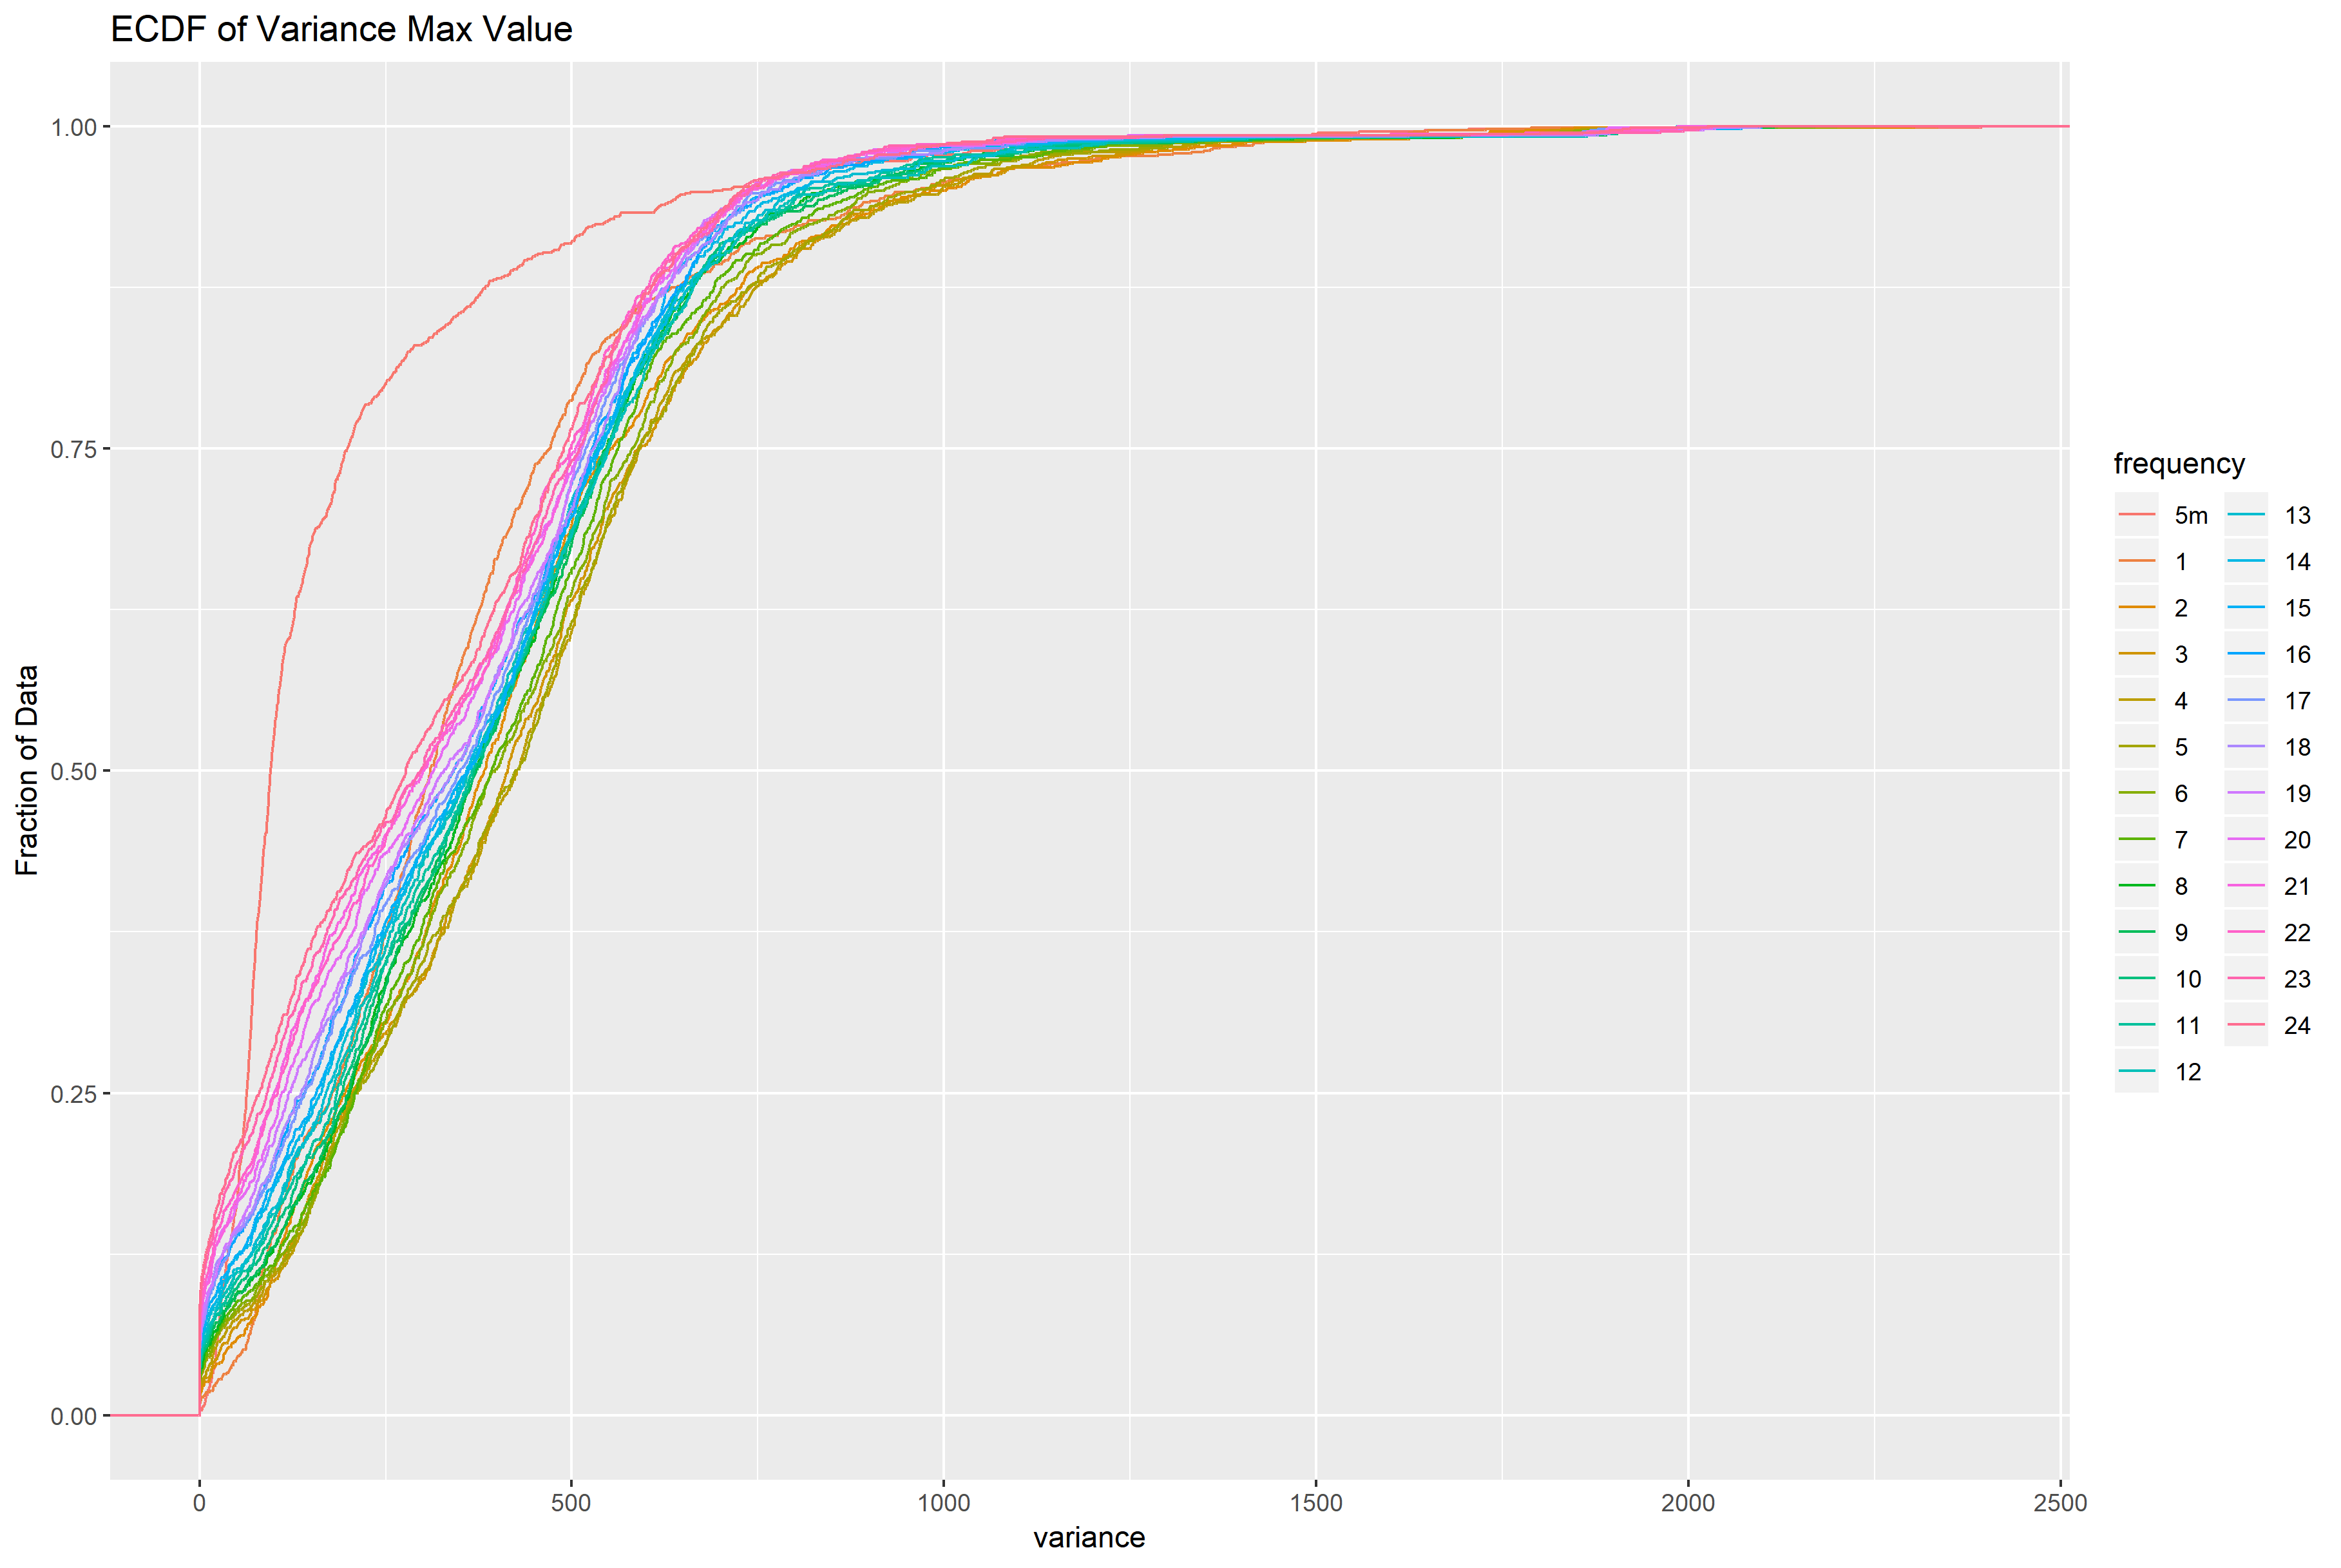
\includegraphics[width = 0.8\textwidth]{ECDFofVarianceMaxValue}
\label{fig:fig1.1.1}
\end{figure}

\begin{figure}[htbp]
\caption{ECDF of CoV of Maxes}
\centering
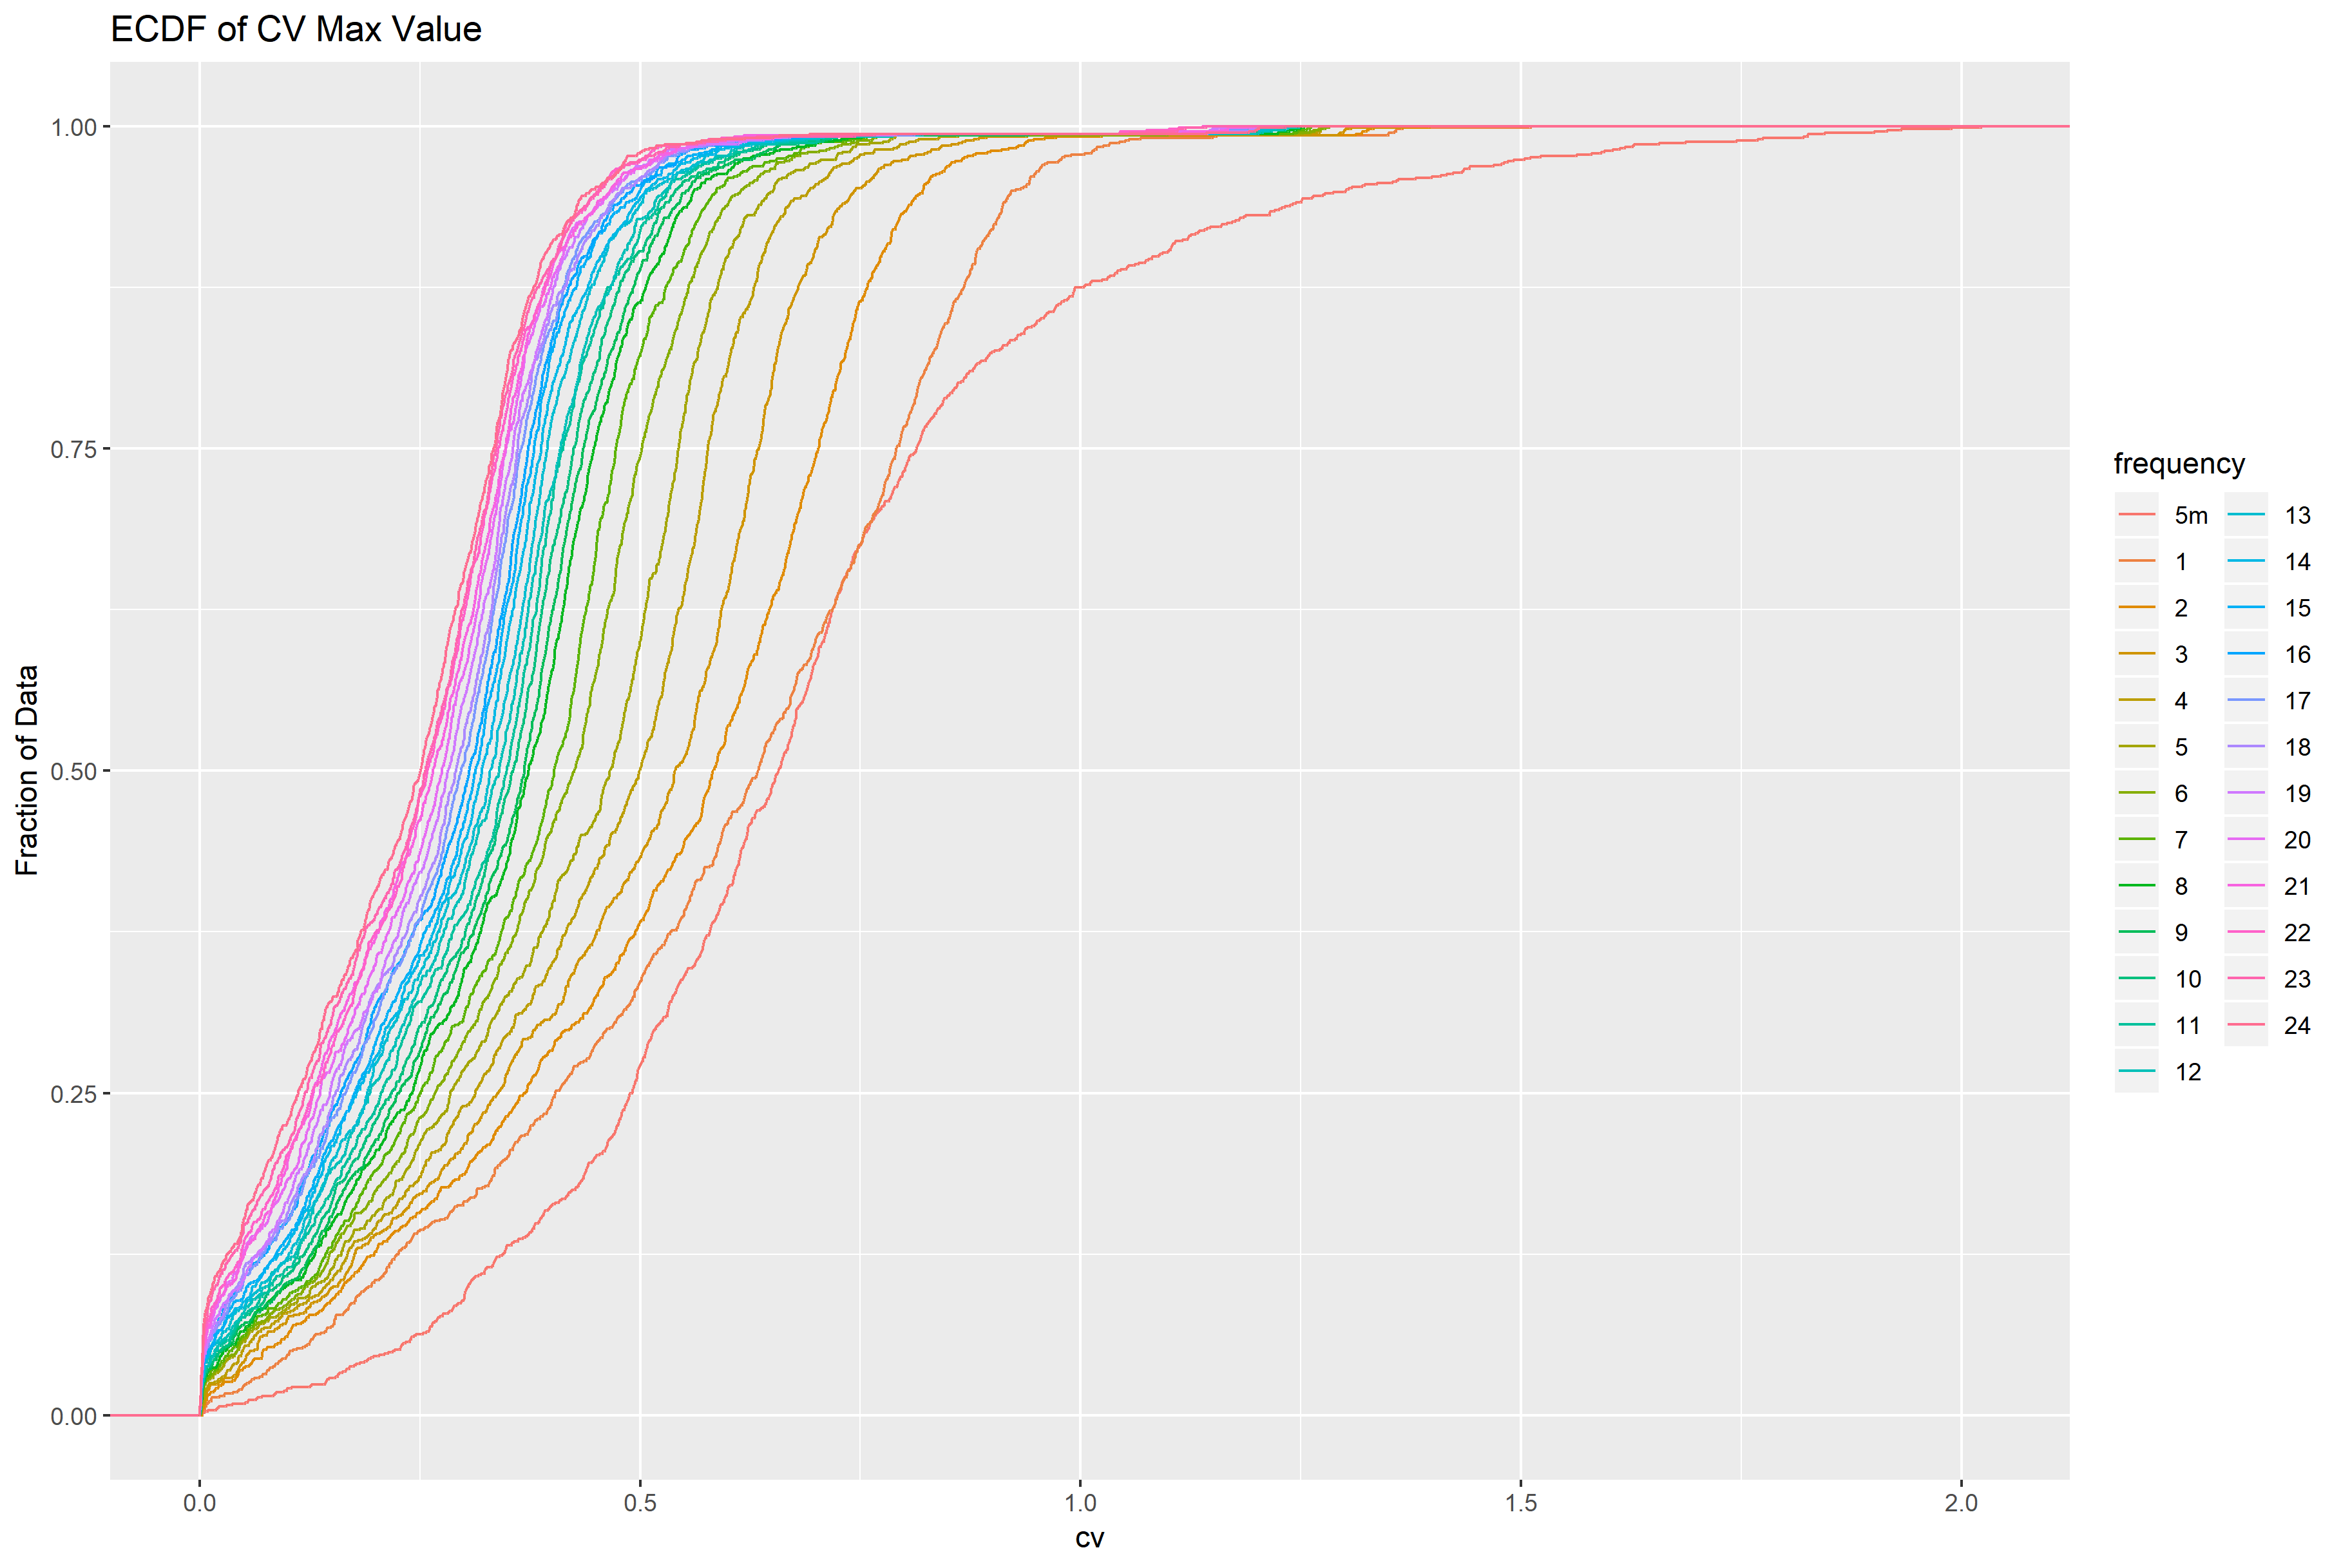
\includegraphics[width = 0.8\textwidth]{ECDFofCVMaxValue}
\label{fig:fig1.1.2}
\end{figure}

\begin{figure}[htbp]
\caption{ECDF of Entropy of Maxes}
\centering
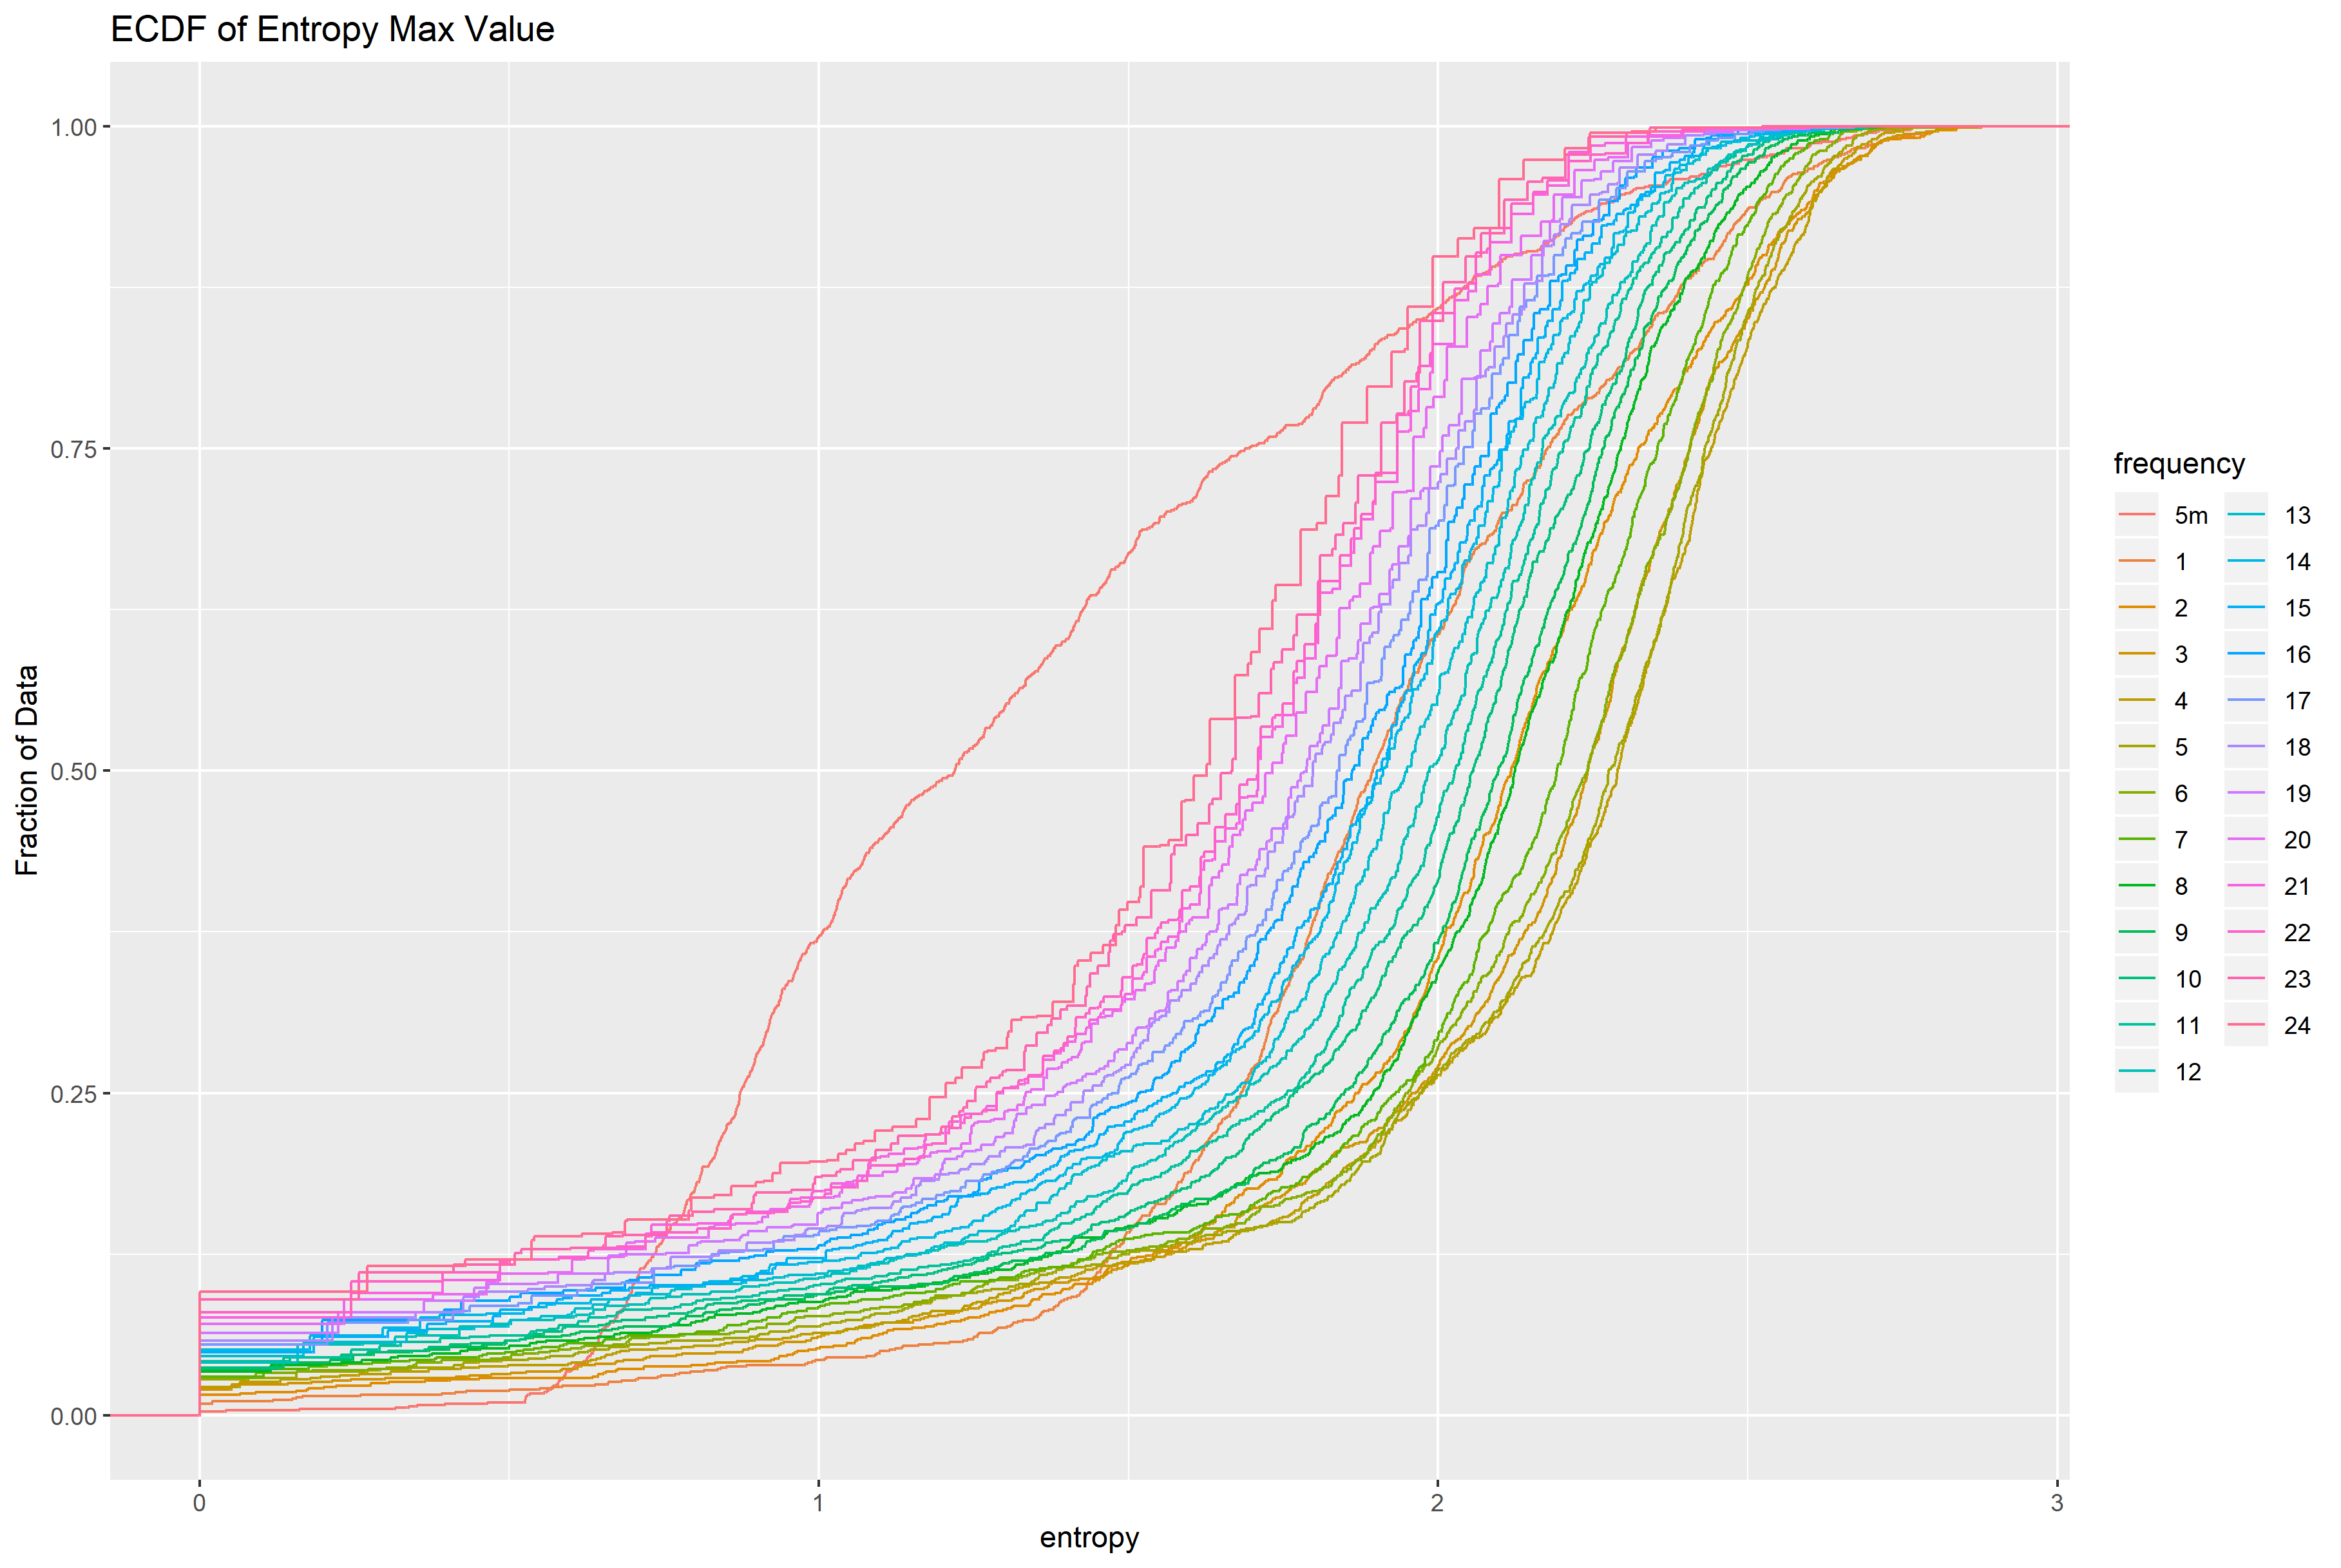
\includegraphics[width = 0.8\textwidth]{ECDFofEntropyMaxValue}
\label{fig:fig1.1.3}
\end{figure}

\begin{figure}[htbp]
\caption{ECDF of Pearson Correlation between Maxes and (Past) Maxes}
\centering
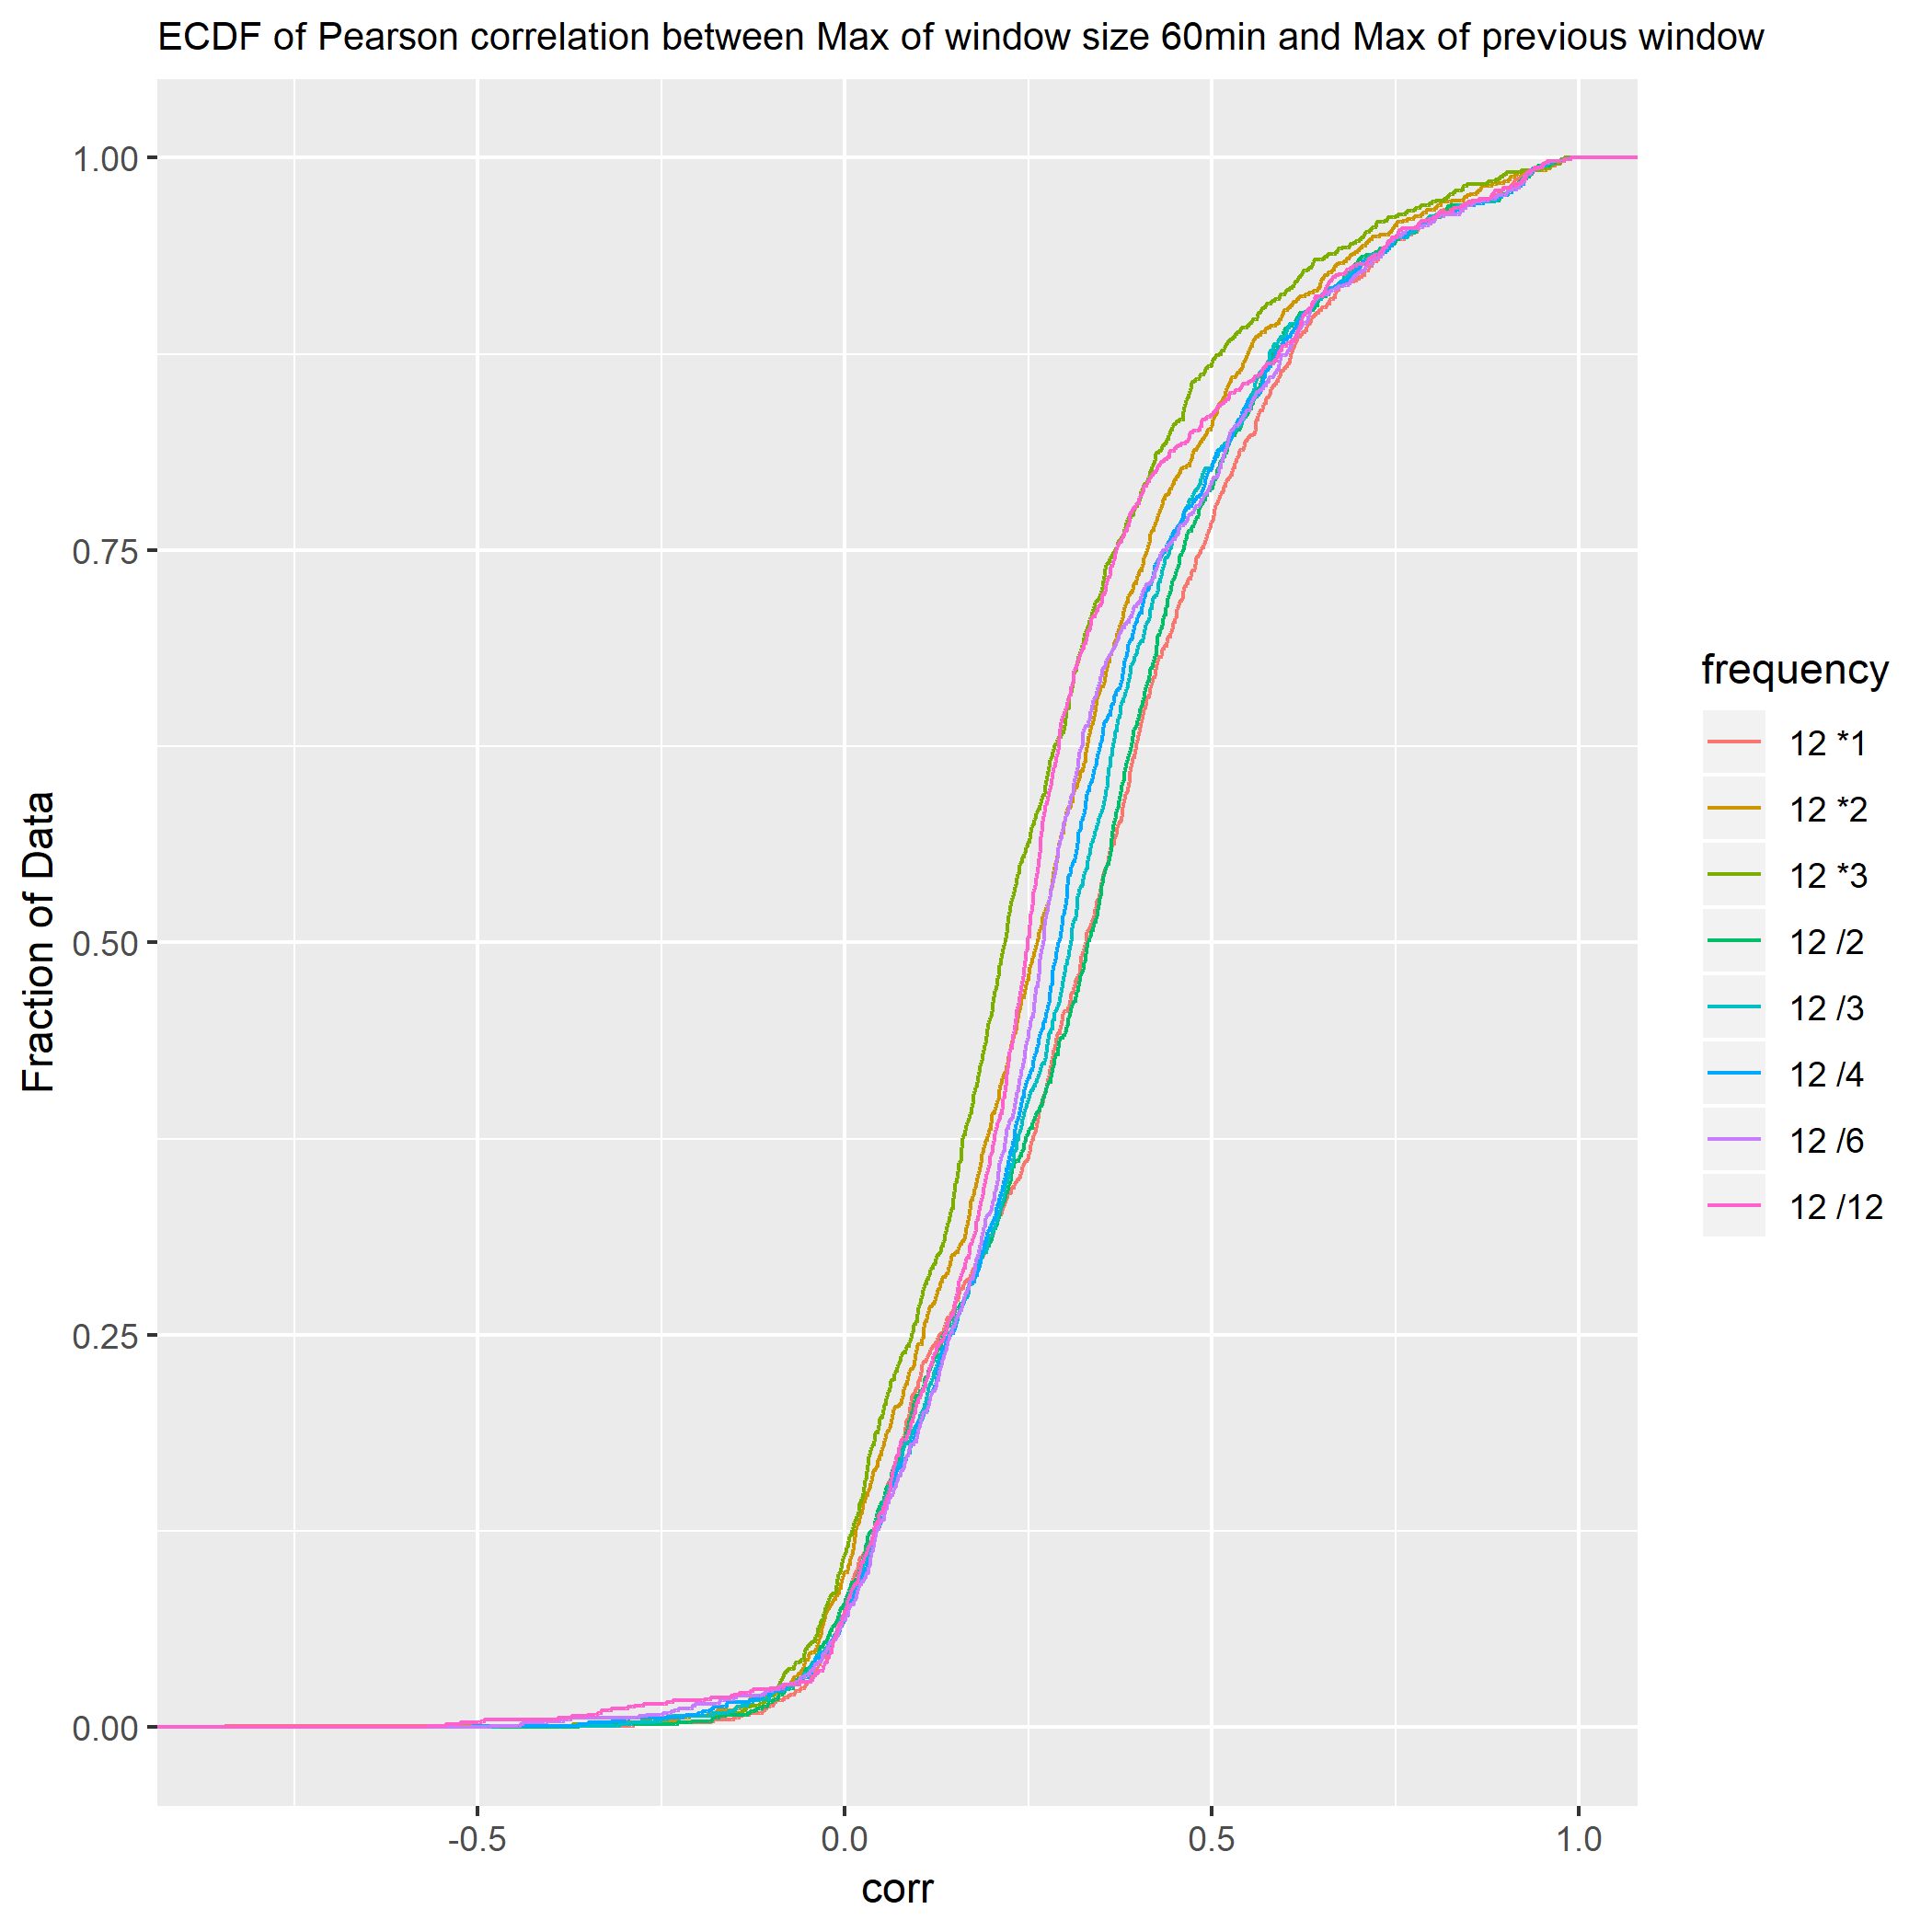
\includegraphics[width = 0.8\textwidth]{ECDFofPearsoncorrelationbetweenMaxofwindowsize60minandMaxofpreviouswindow}
\label{fig:fig1.1.4}
\end{figure}

\begin{figure}[htbp]
\caption{ECDF of Pearson Correlation between Maxes and (Past) Avgs}
\centering
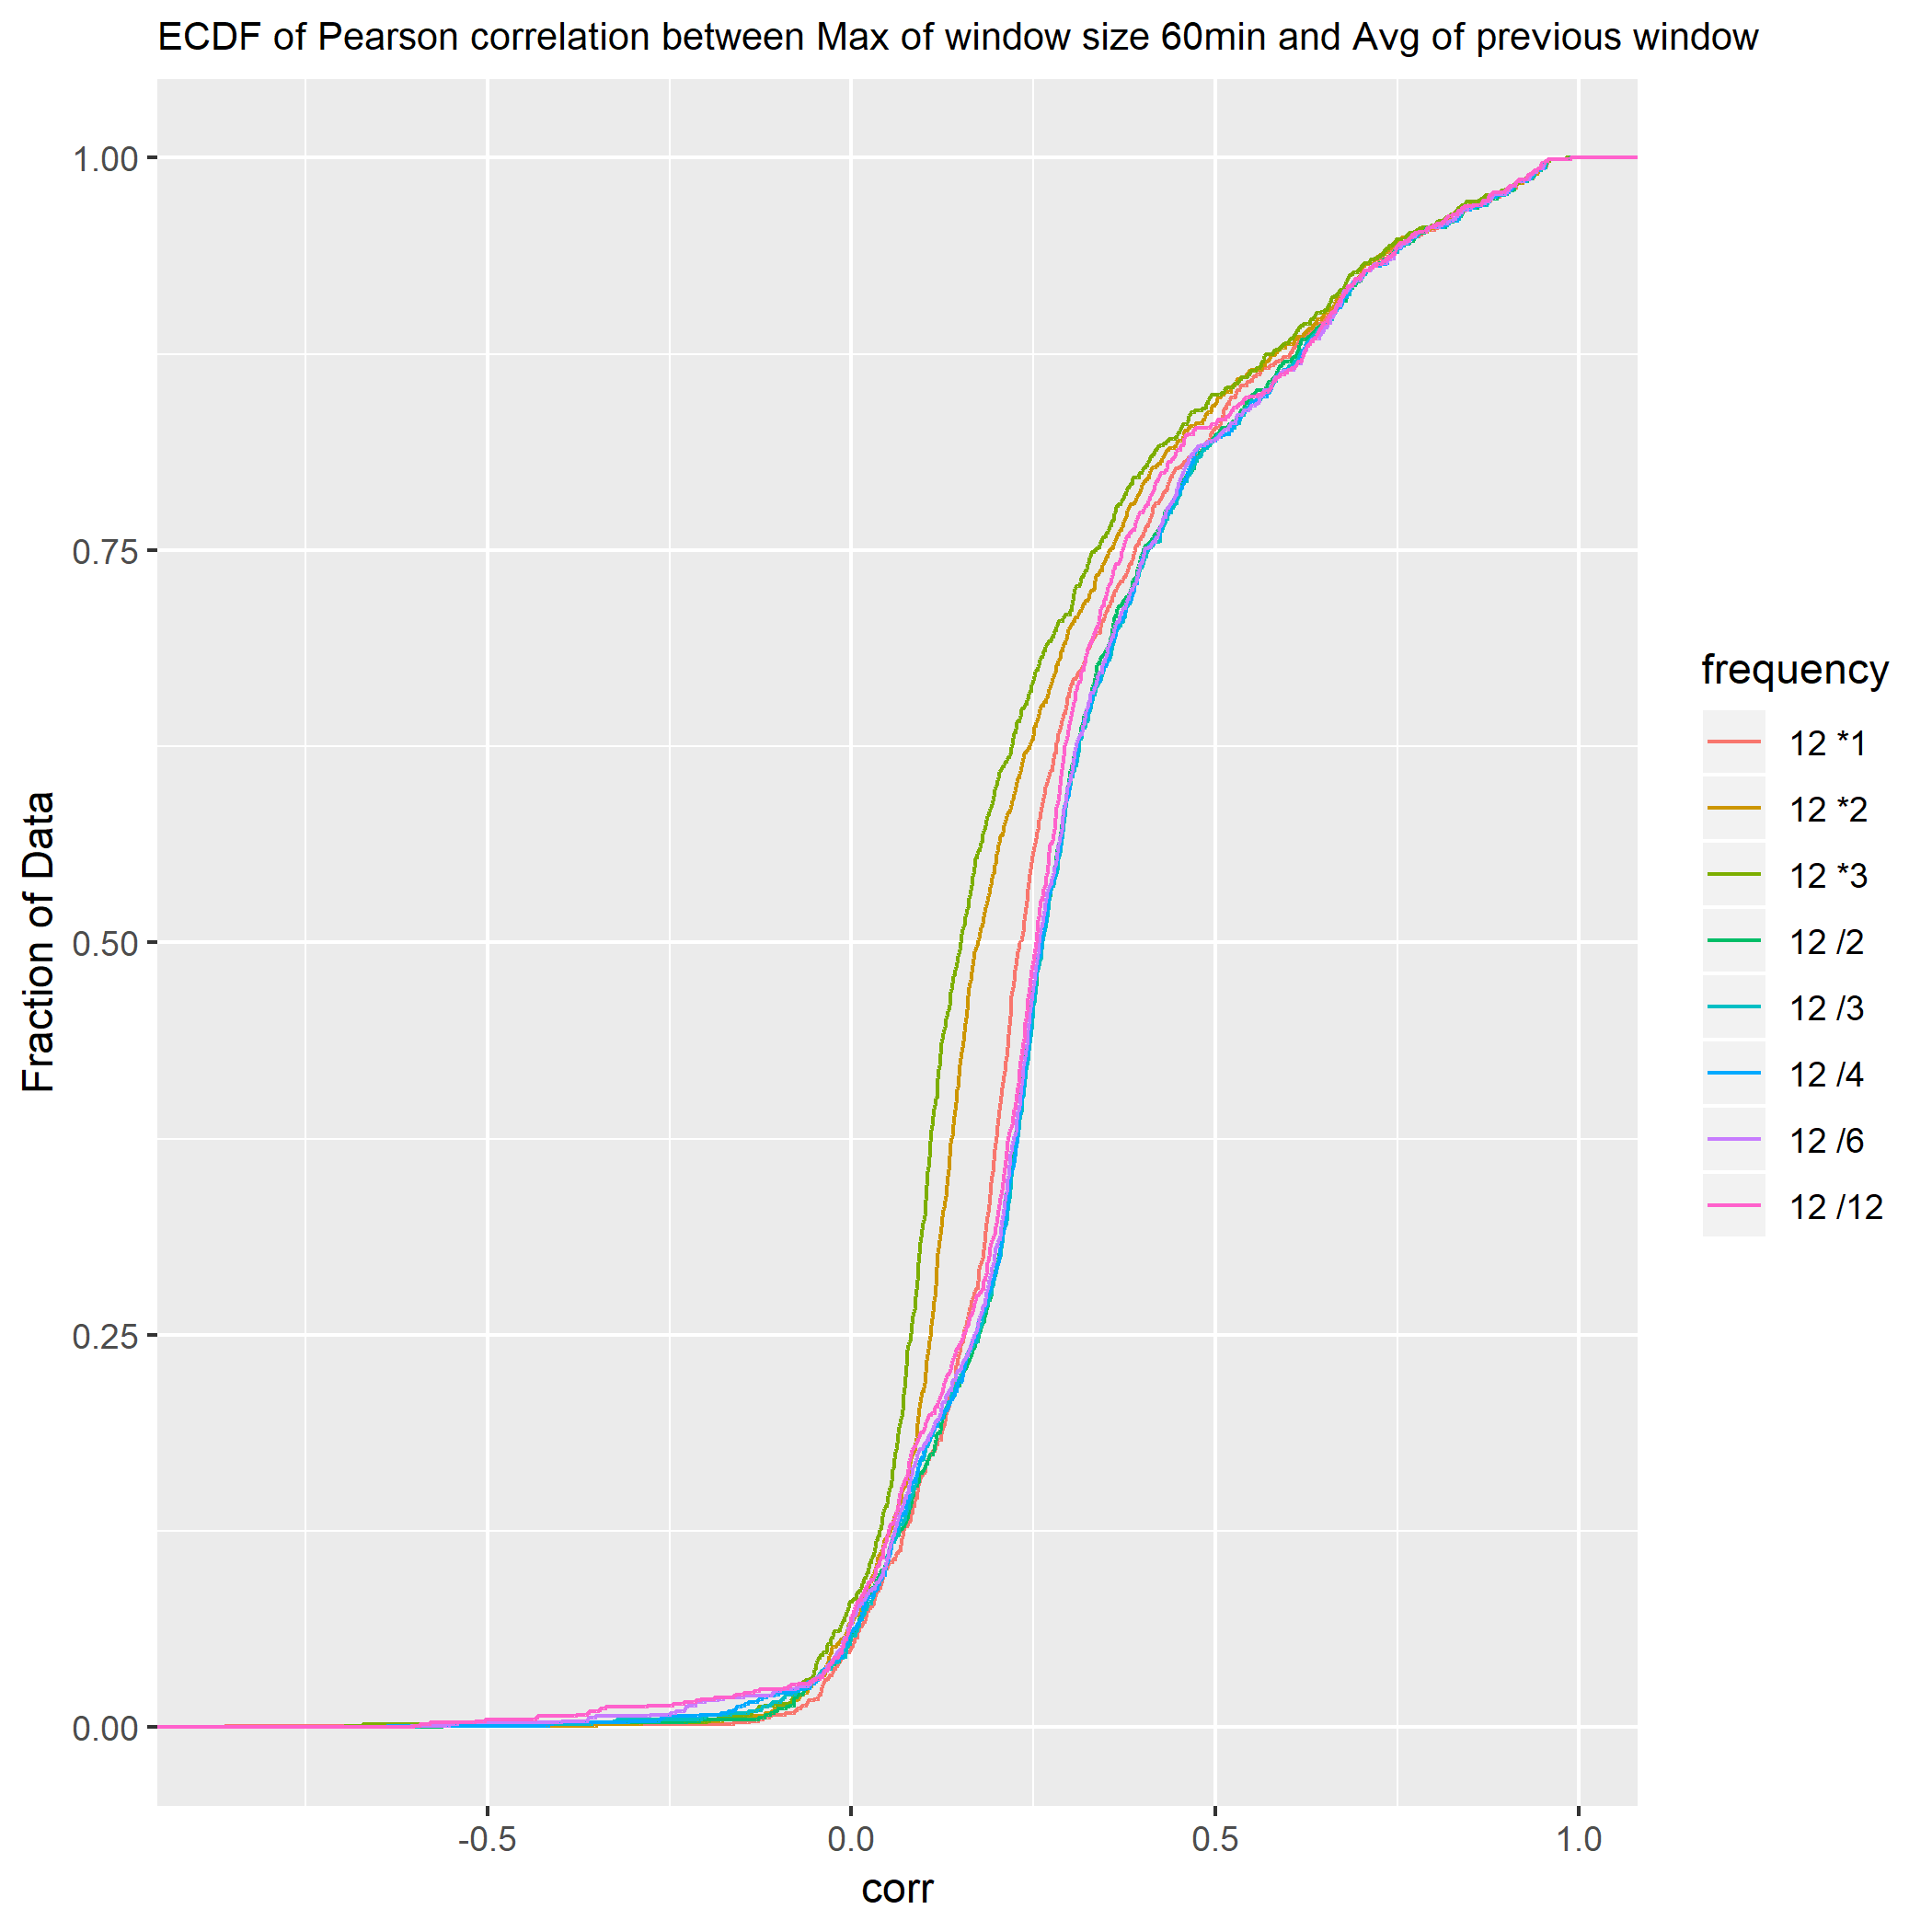
\includegraphics[width = 0.8\textwidth]{ECDFofPearsoncorrelationbetweenMaxofwindowsize60minandAvgofpreviouswindow}
\label{fig:fig1.1.5}
\end{figure}

\begin{figure}[htbp]
\caption{ECDF of Pearson Correlation between Maxes and (Past) Average of Maxes}
\centering
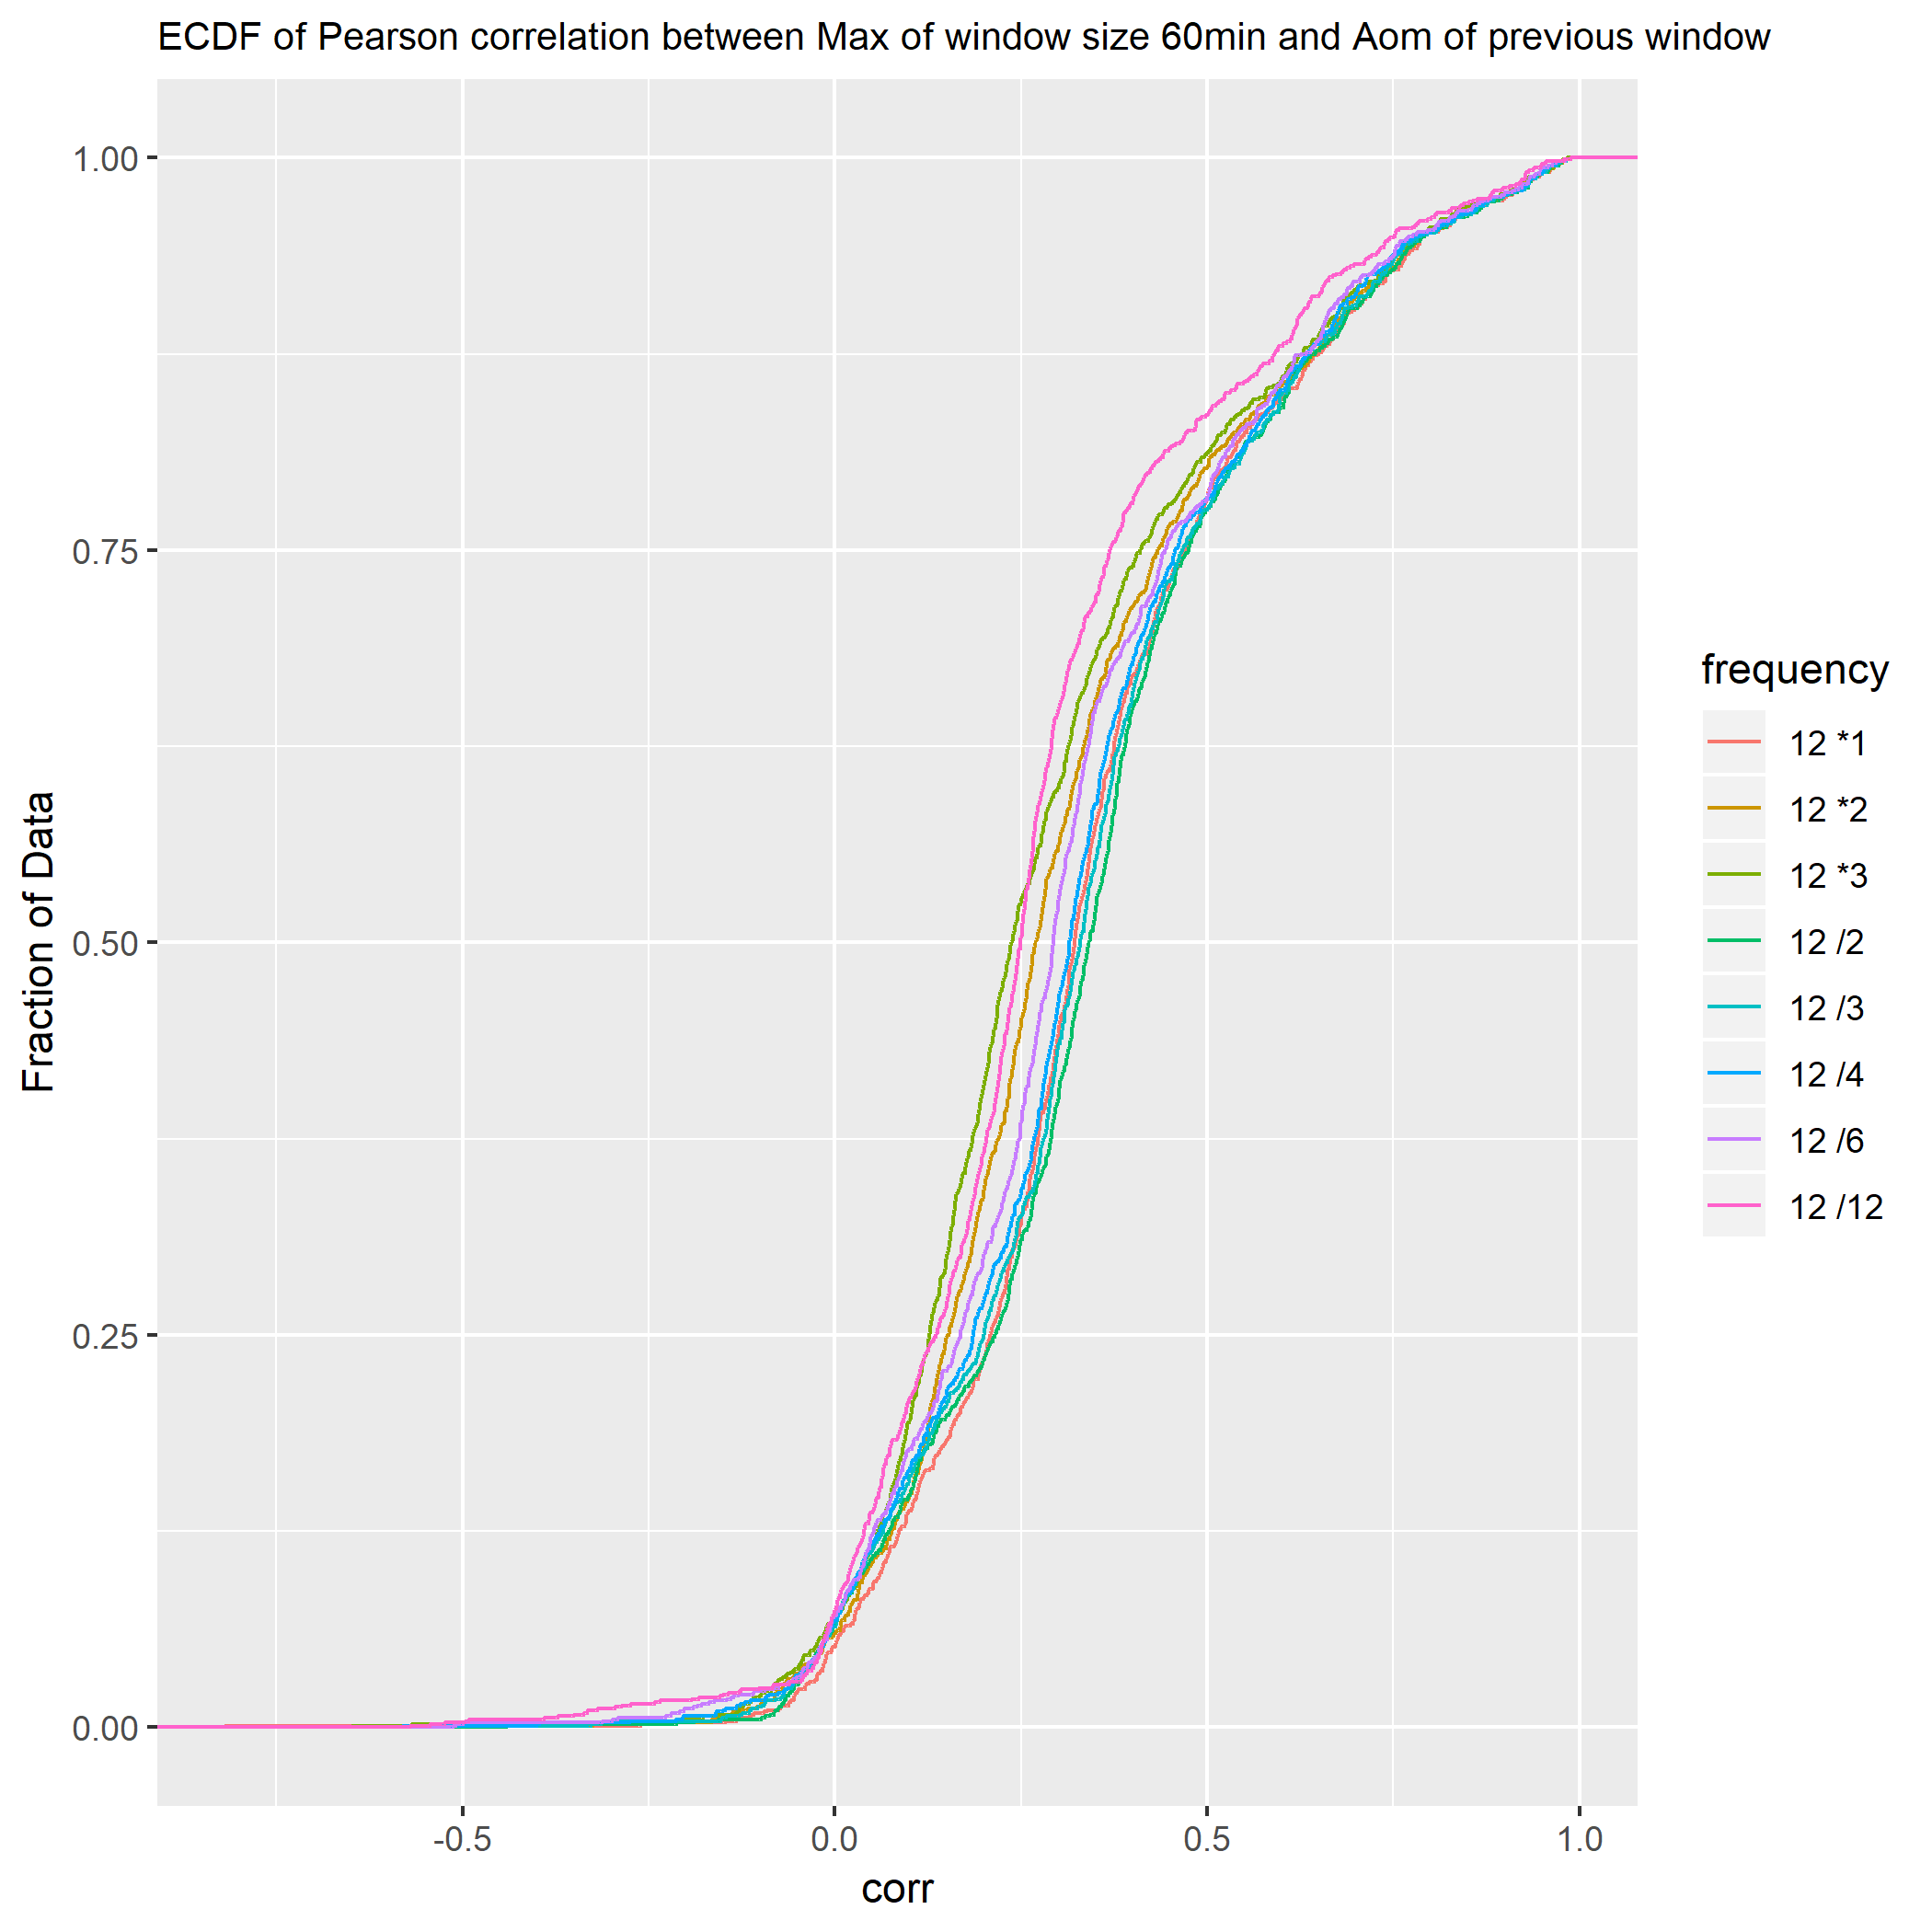
\includegraphics[width = 0.8\textwidth]{ECDFofPearsoncorrelationbetweenMaxofwindowsize60minandAomofpreviouswindow}
\label{fig:fig1.1.6}
\end{figure}

\subsubsection{Cut-off Probability}
Ref to Section 1.2, include Fig \ref{fig:fig1.2.1}, Table \ref{tab:tab1.2.1}.

\begin{figure}
    \caption{Trade-off Curve for AR1 Model With Offline Training}
    \centering
    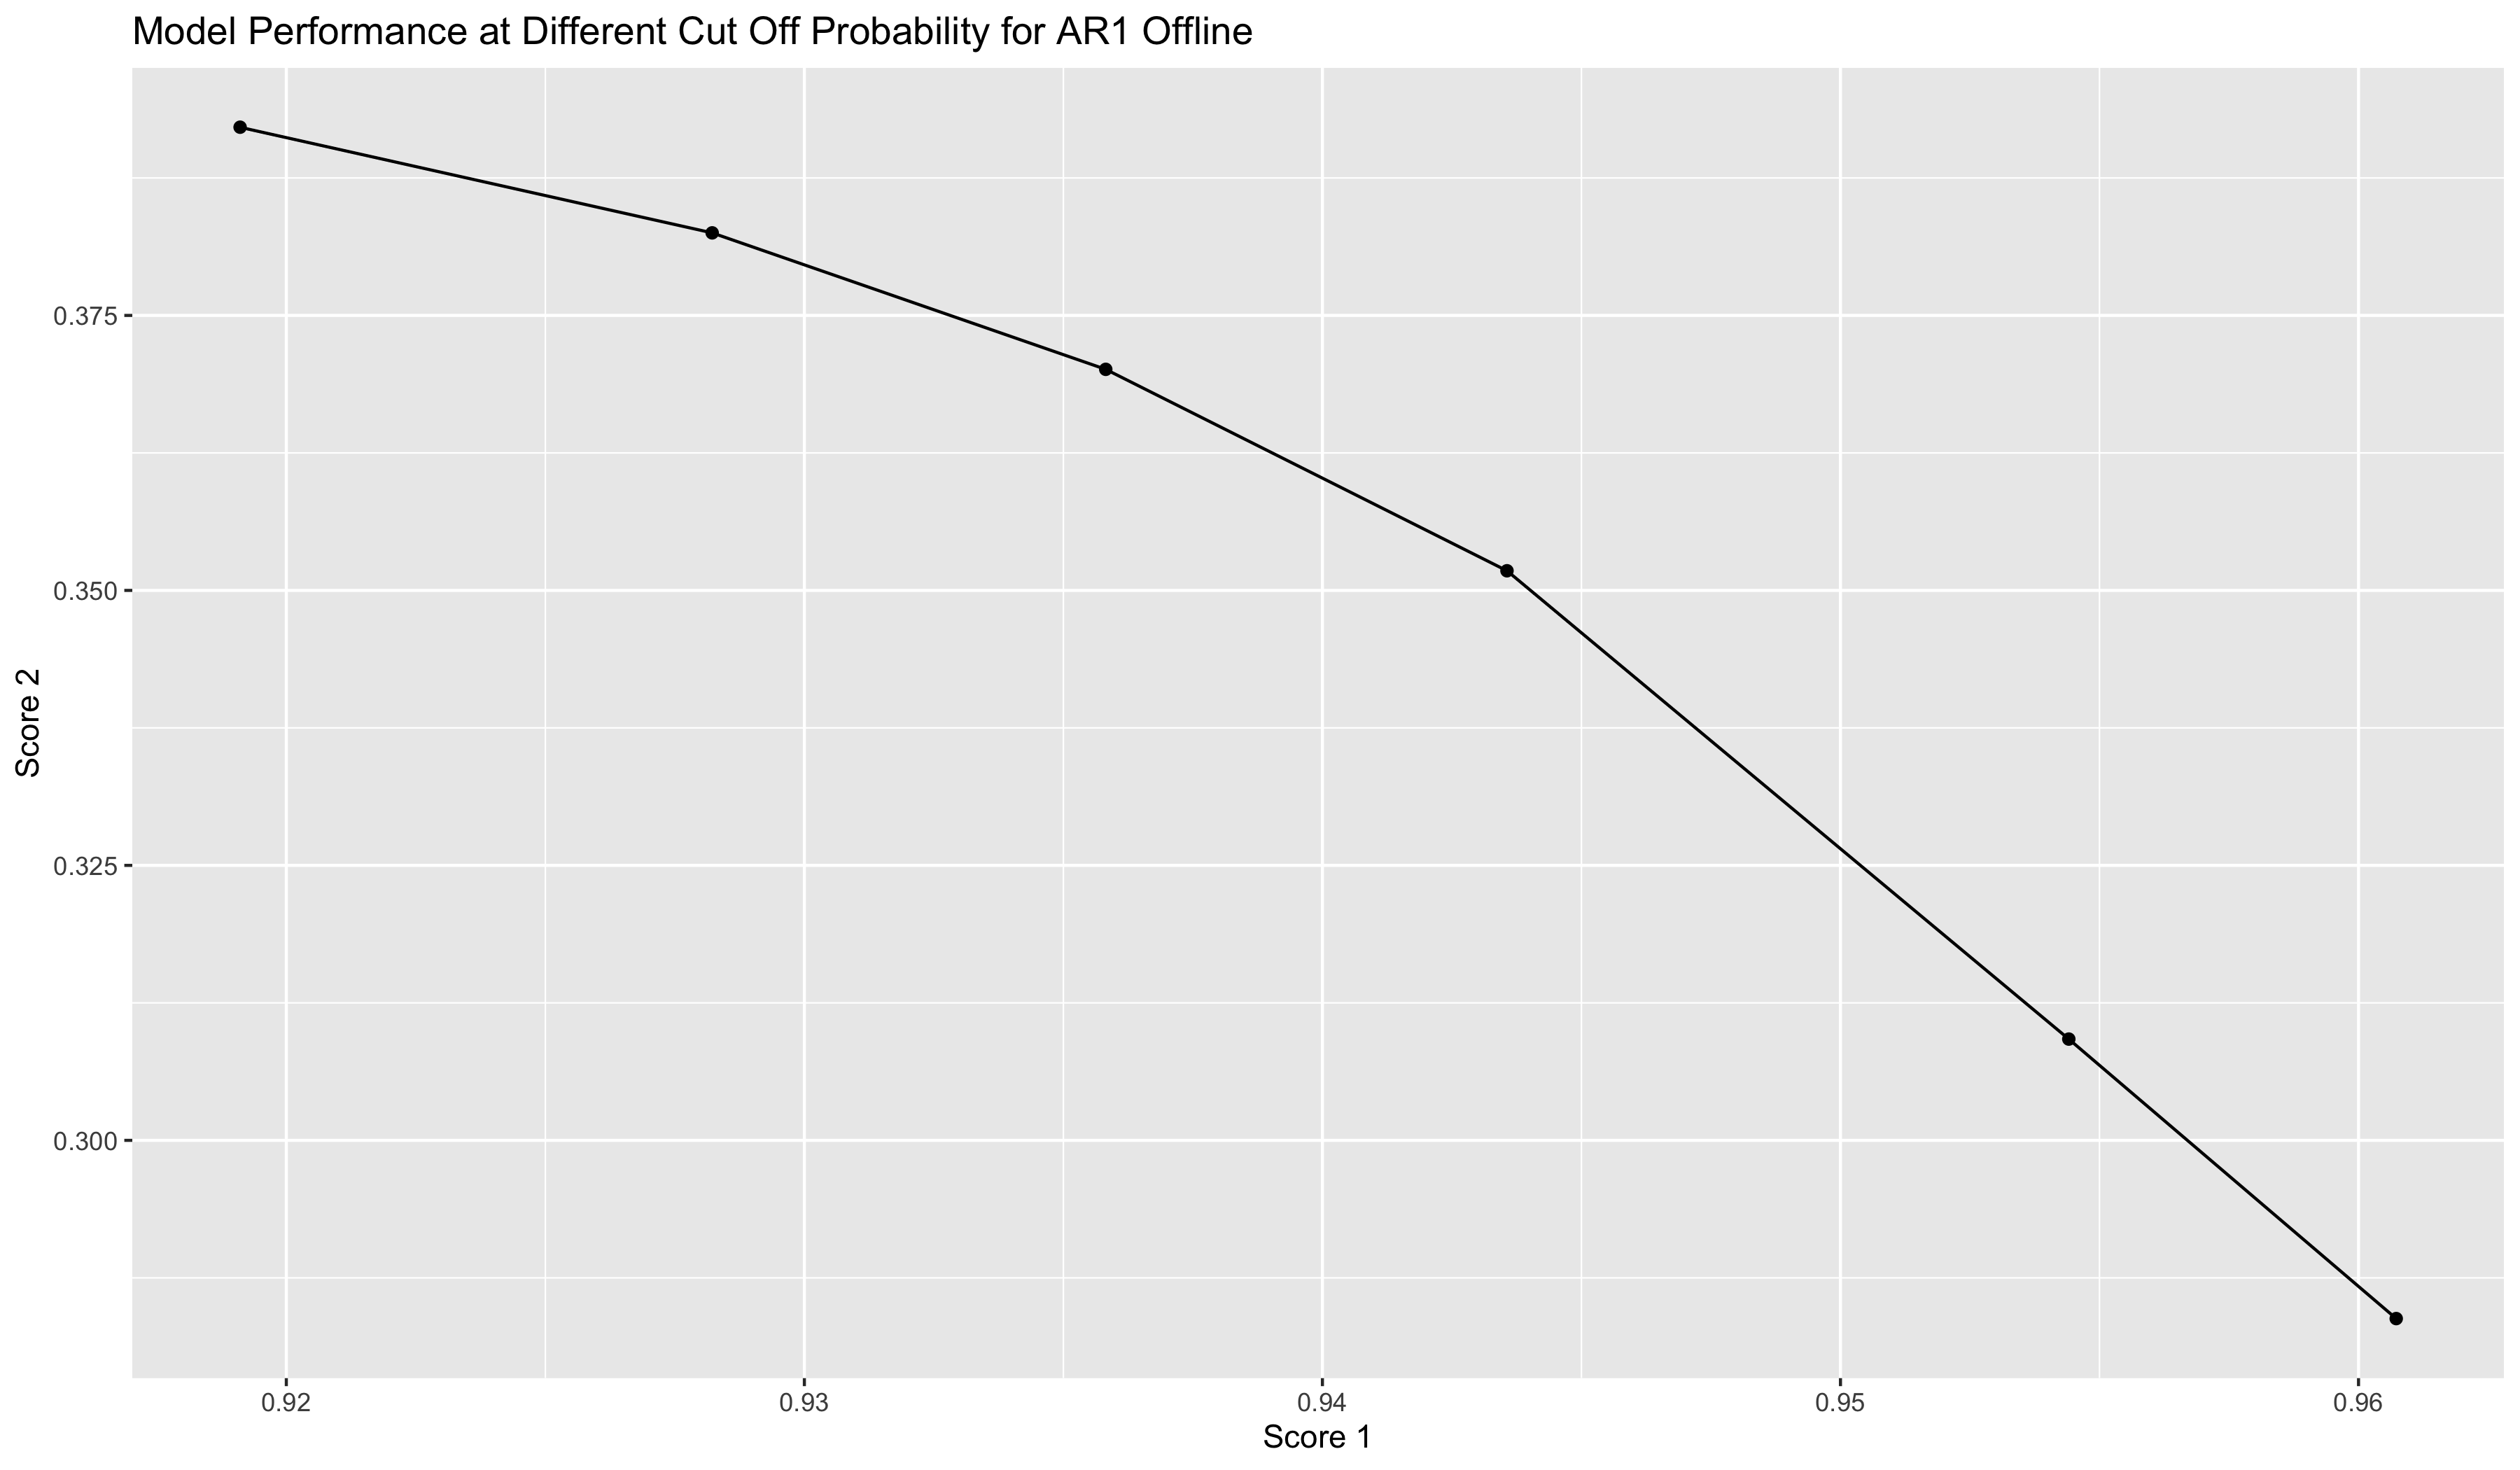
\includegraphics{images/ModelPerformanceatDifferentCutOffProbabilityforAR1Offline.png}
    \label{fig:fig1.2.1}
\end{figure}

\begin{table}[htbp]
  \begin{center}
    \caption{Configuration and Result of AR1 Model with Different Cut Off Probability of Offline Training}
    \label{tab:tab1.2.1}
    \begin{tabular}{l|*{4}{c}} \textbf{cut off prob} & \textbf{score 1} &
      \textbf{score 1 weight} & \textbf{score 2} & \textbf{score 2 weight} \\
      \hline
      0.005 & 0.9277 & 47487 & 0.3142 & 59249\\
      0.01 & 0.9168 & 48124 & 0.3463 & 59249\\
      0.03 & 0.8965 & 50300 & 0.4024 & 59249\\
      0.05 & 0.8841 & 52904 & 0.4309 & 59249\\
      0.07 & 0.8706 & 53640 & 0.4518 & 59249\\
      0.10 & 0.8548 & 54444 & 0.4729 & 59249\\
    \end{tabular}
  \end{center}
\end{table}


\subsubsection{Models}
Ref to Section 1.3, include Fig \ref{fig:fig1.3.1}, Table \ref{tab:tab1.3.1},
Fig \ref{fig:fig1.3.2}, Table \ref{tab:tab1.3.2}, Fig \ref{fig:fig1.3.3}, Table
\ref{tab:tab1.3.3}, Fig \ref{fig:fig1.3.4}, Table \ref{tab:tab1.3.4}, Fig
\ref{fig:fig1.3.5}, Table \ref{tab:tab1.3.5}, Fig \ref{fig:fig1.3.6}, Table
\ref{tab:tab1.3.6}, Fig \ref{fig:fig1.3.7}, Table \ref{tab:tab1.3.7}.

\begin{figure}[htbp]
    \caption{Trade-off Curves for ARIMA-like Models with Offline Training}
    \centering
    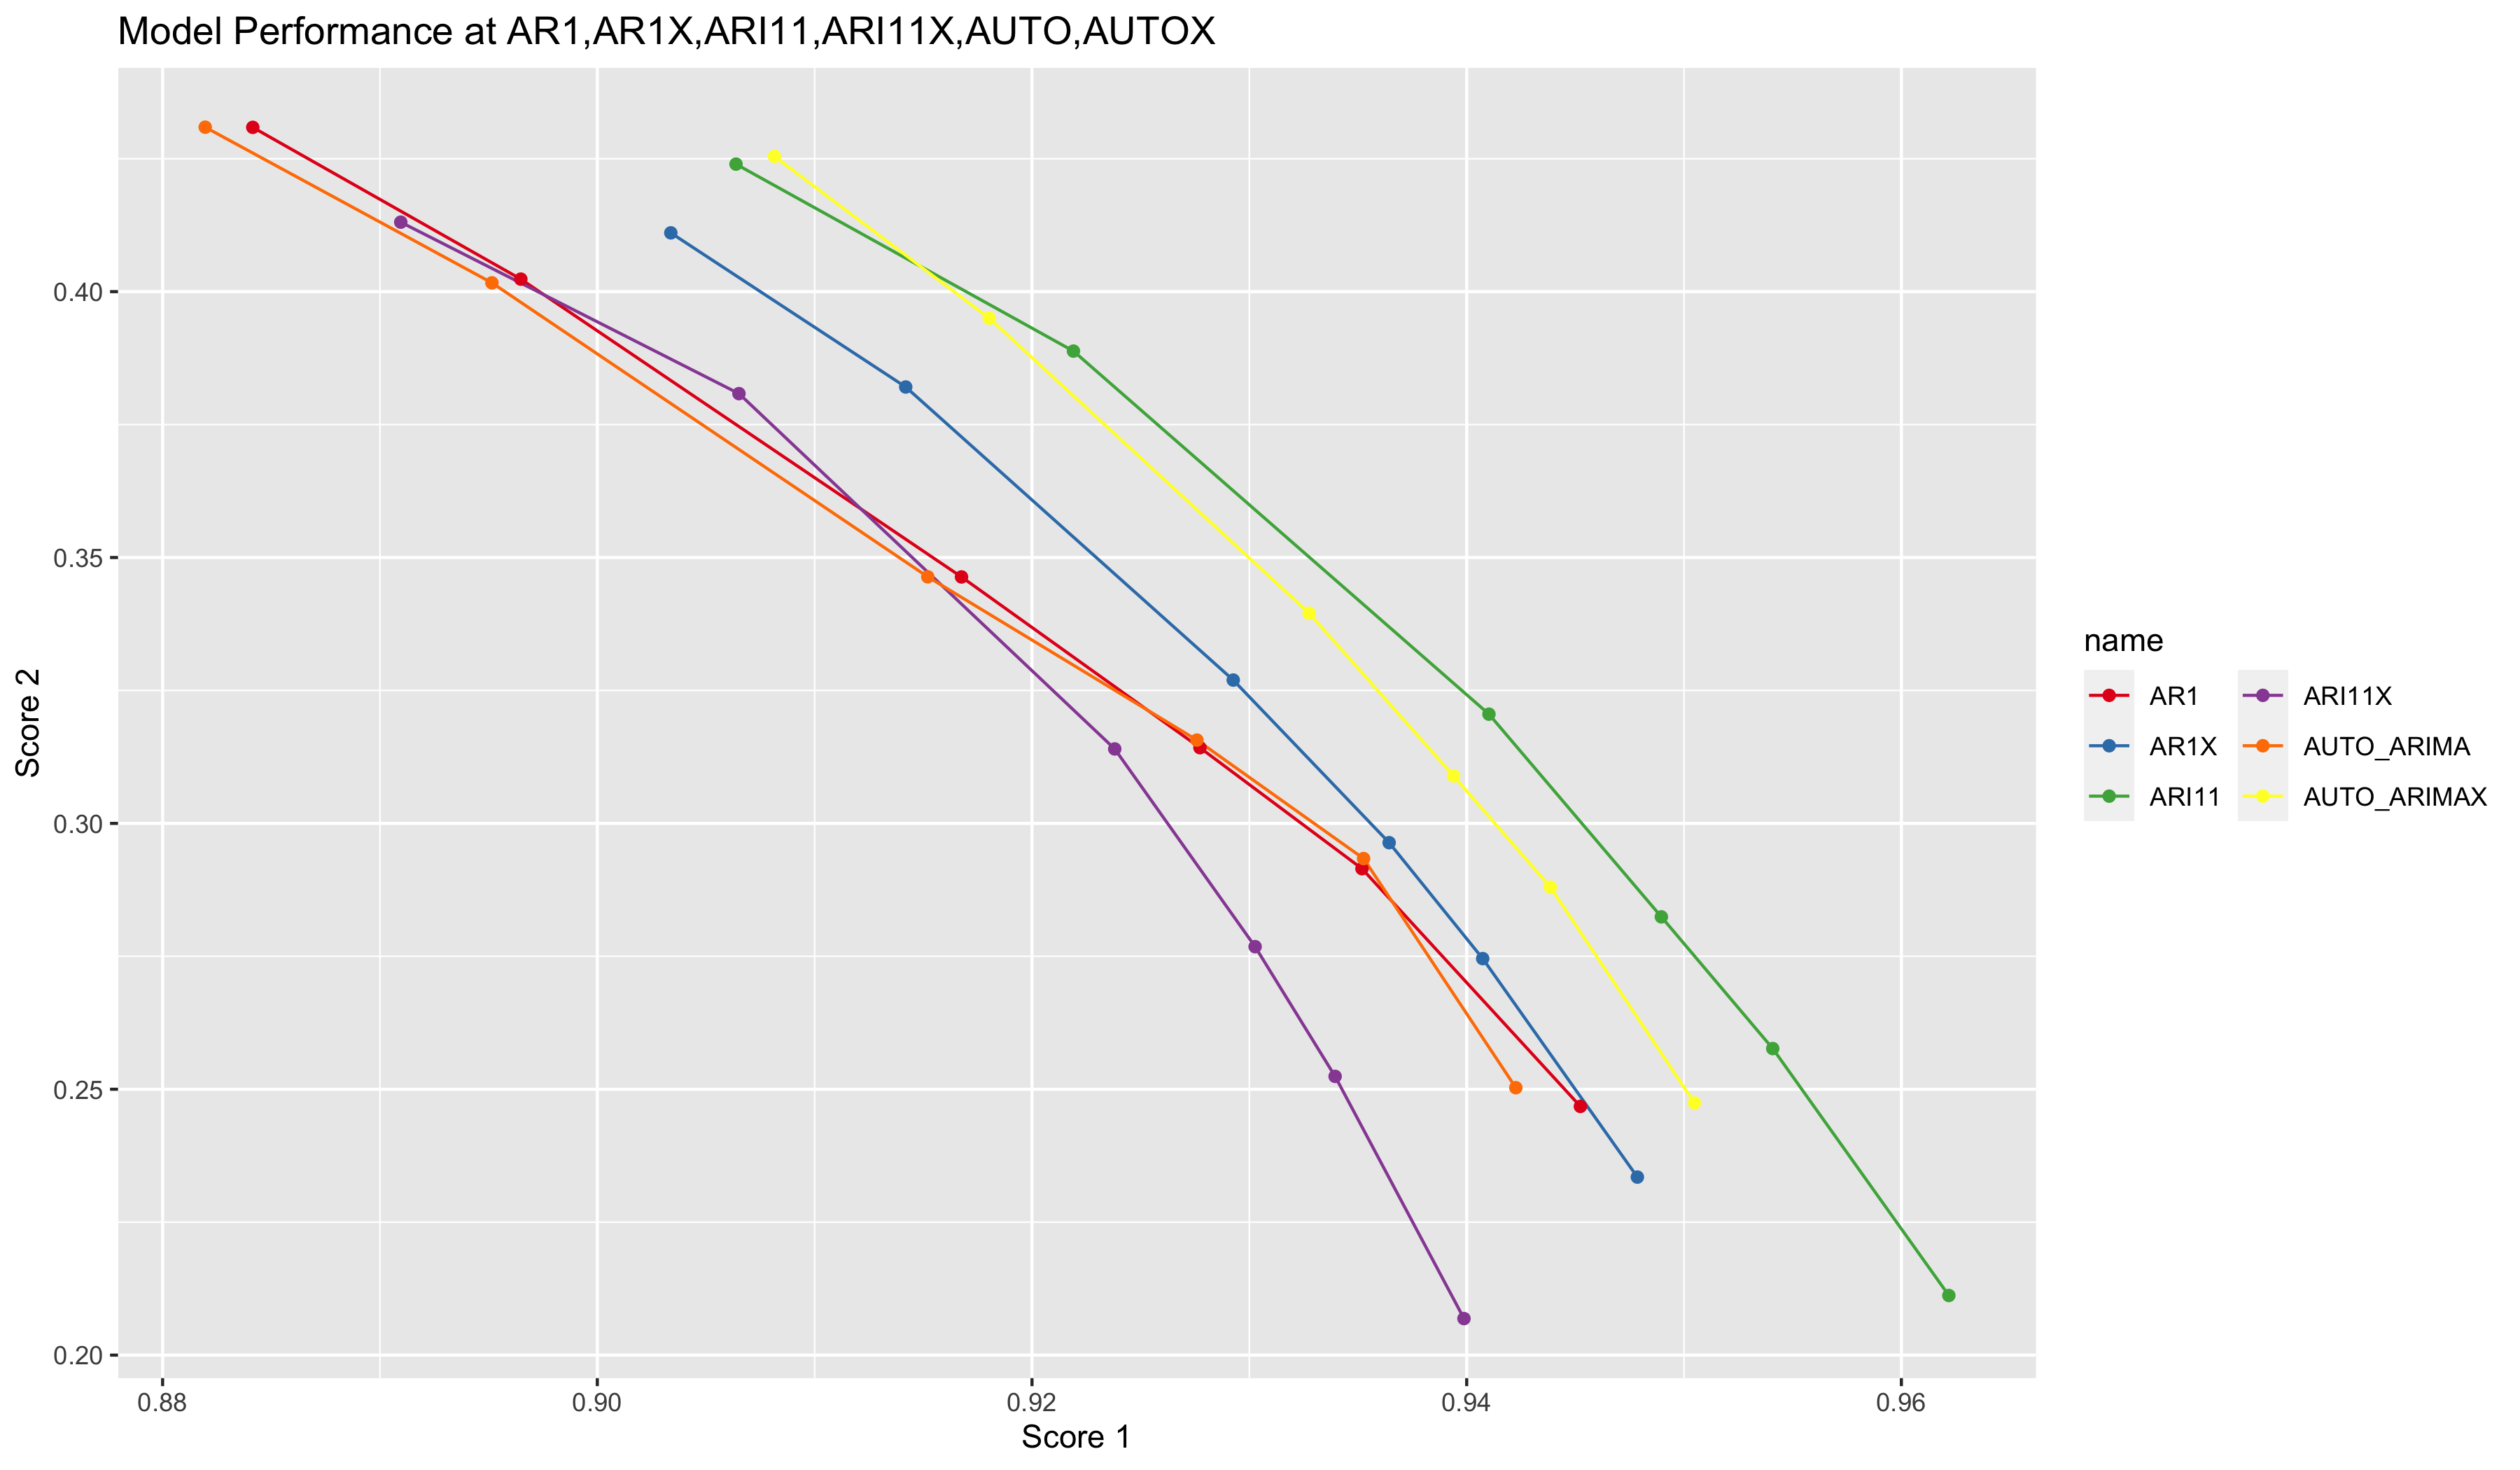
\includegraphics[width = 0.8\textwidth]{images/ModelPerformanceatAR1,AR1X,ARI11,ARI11X,AUTO,AUTOX.png}
    \label{fig:fig1.3.1}
\end{figure}

\begin{longtable}[htbp]{l|l|*{4}{c}}
    \caption{Configuration and Result of ARI11,ARI11X Models with Offline Training}
    \label{tab:tab1.3.1} \\
    \textbf{name} & \textbf{cut off prob} & \textbf{score 1} & \textbf{score 1
    weight} & \textbf{score 2} & \textbf{score 2 weight}\\
    \hline
    AR1 & 0.001 & 0.9452 & 42981 & 0.2468 & 59249\\
    AR1 & 0.003 & 0.9352 & 46484 & 0.2915 & 59249\\
    AR1 & 0.005 & 0.9277 & 47487 & 0.3142 & 59249\\
    AR1 & 0.010 & 0.9168 & 48124 & 0.3463 & 59249\\
    AR1 & 0.030 & 0.8965 & 50300 & 0.4024 & 59249\\
    AR1 & 0.050 & 0.8841 & 52904 & 0.4309 & 59249\\
    AR1X & 0.001 & 0.9479 & 41306 & 0.2335 & 59249\\
    AR1X & 0.003 & 0.9407 & 43602 & 0.2746 & 59249\\
    AR1X & 0.005 & 0.9364 & 44299 & 0.2964 & 59249\\
    AR1X & 0.010 & 0.9293 & 45094 & 0.3270 & 59249\\
    AR1X & 0.030 & 0.9142 & 47570 & 0.3821 & 59249\\
    AR1X & 0.050 & 0.9034 & 50374 & 0.4111 & 59249\\
    ARI11 & 0.001 & 0.9622 & 37735 & 0.2112 & 59249\\
    ARI11 & 0.003 & 0.9541 & 42205 & 0.2576 & 59249\\
    ARI11 & 0.005 & 0.9490 & 44002 & 0.2824 & 59249\\
    ARI11 & 0.010 & 0.9410 & 46307 & 0.3205 & 59249\\
    ARI11 & 0.030 & 0.9219 & 48903 & 0.3888 & 59249\\
    ARI11 & 0.050 & 0.9064 & 50471 & 0.4240 & 59249\\
    ARI11X & 0.001 & 0.9399 & 38470 & 0.2069 & 59249\\
    ARI11X & 0.003 & 0.9339 & 42132 & 0.2524 & 59249\\
    ARI11X & 0.005 & 0.9303 & 43794 & 0.2768 & 59249\\
    ARI11X & 0.010 & 0.9238 & 45778 & 0.3140 & 59249\\
    ARI11X & 0.030 & 0.9065 & 48501 & 0.3808 & 59249\\
    ARI11X & 0.050 & 0.8910 & 49852 & 0.4131 & 59249\\
    AUTO & 0.001 & 0.9423 & 41566 & 0.2503 & 59249\\
    AUTO & 0.003 & 0.9353 & 46182 & 0.2934 & 59249\\
    AUTO & 0.005 & 0.9276 & 46954 & 0.3157 & 59249\\
    AUTO & 0.010 & 0.9152 & 47691 & 0.3464 & 59249\\
    AUTO & 0.030 & 0.8952 & 50206 & 0.4017 & 59249\\
    AUTO & 0.050 & 0.8820 & 52677 & 0.4309 & 59249\\
    AUTOX & 0.001 & 0.9505 & 41296 & 0.2474 & 59249\\
    AUTOX & 0.003 & 0.9439 & 43562 & 0.2880 & 59249\\
    AUTOX & 0.005 & 0.9394 & 44203 & 0.3089 & 59249\\
    AUTOX & 0.010 & 0.9328 & 45502 & 0.3395 & 59249\\
    AUTOX & 0.030 & 0.9180 & 48421 & 0.3950 & 59249\\
    AUTOX & 0.050 & 0.9082 & 51563 & 0.4254 & 59249\\
\end{longtable}

\begin{figure}[htbp]
    \caption{Trade-off Curves for AR1 with Different Residual Distribution Estimation}
    \centering
    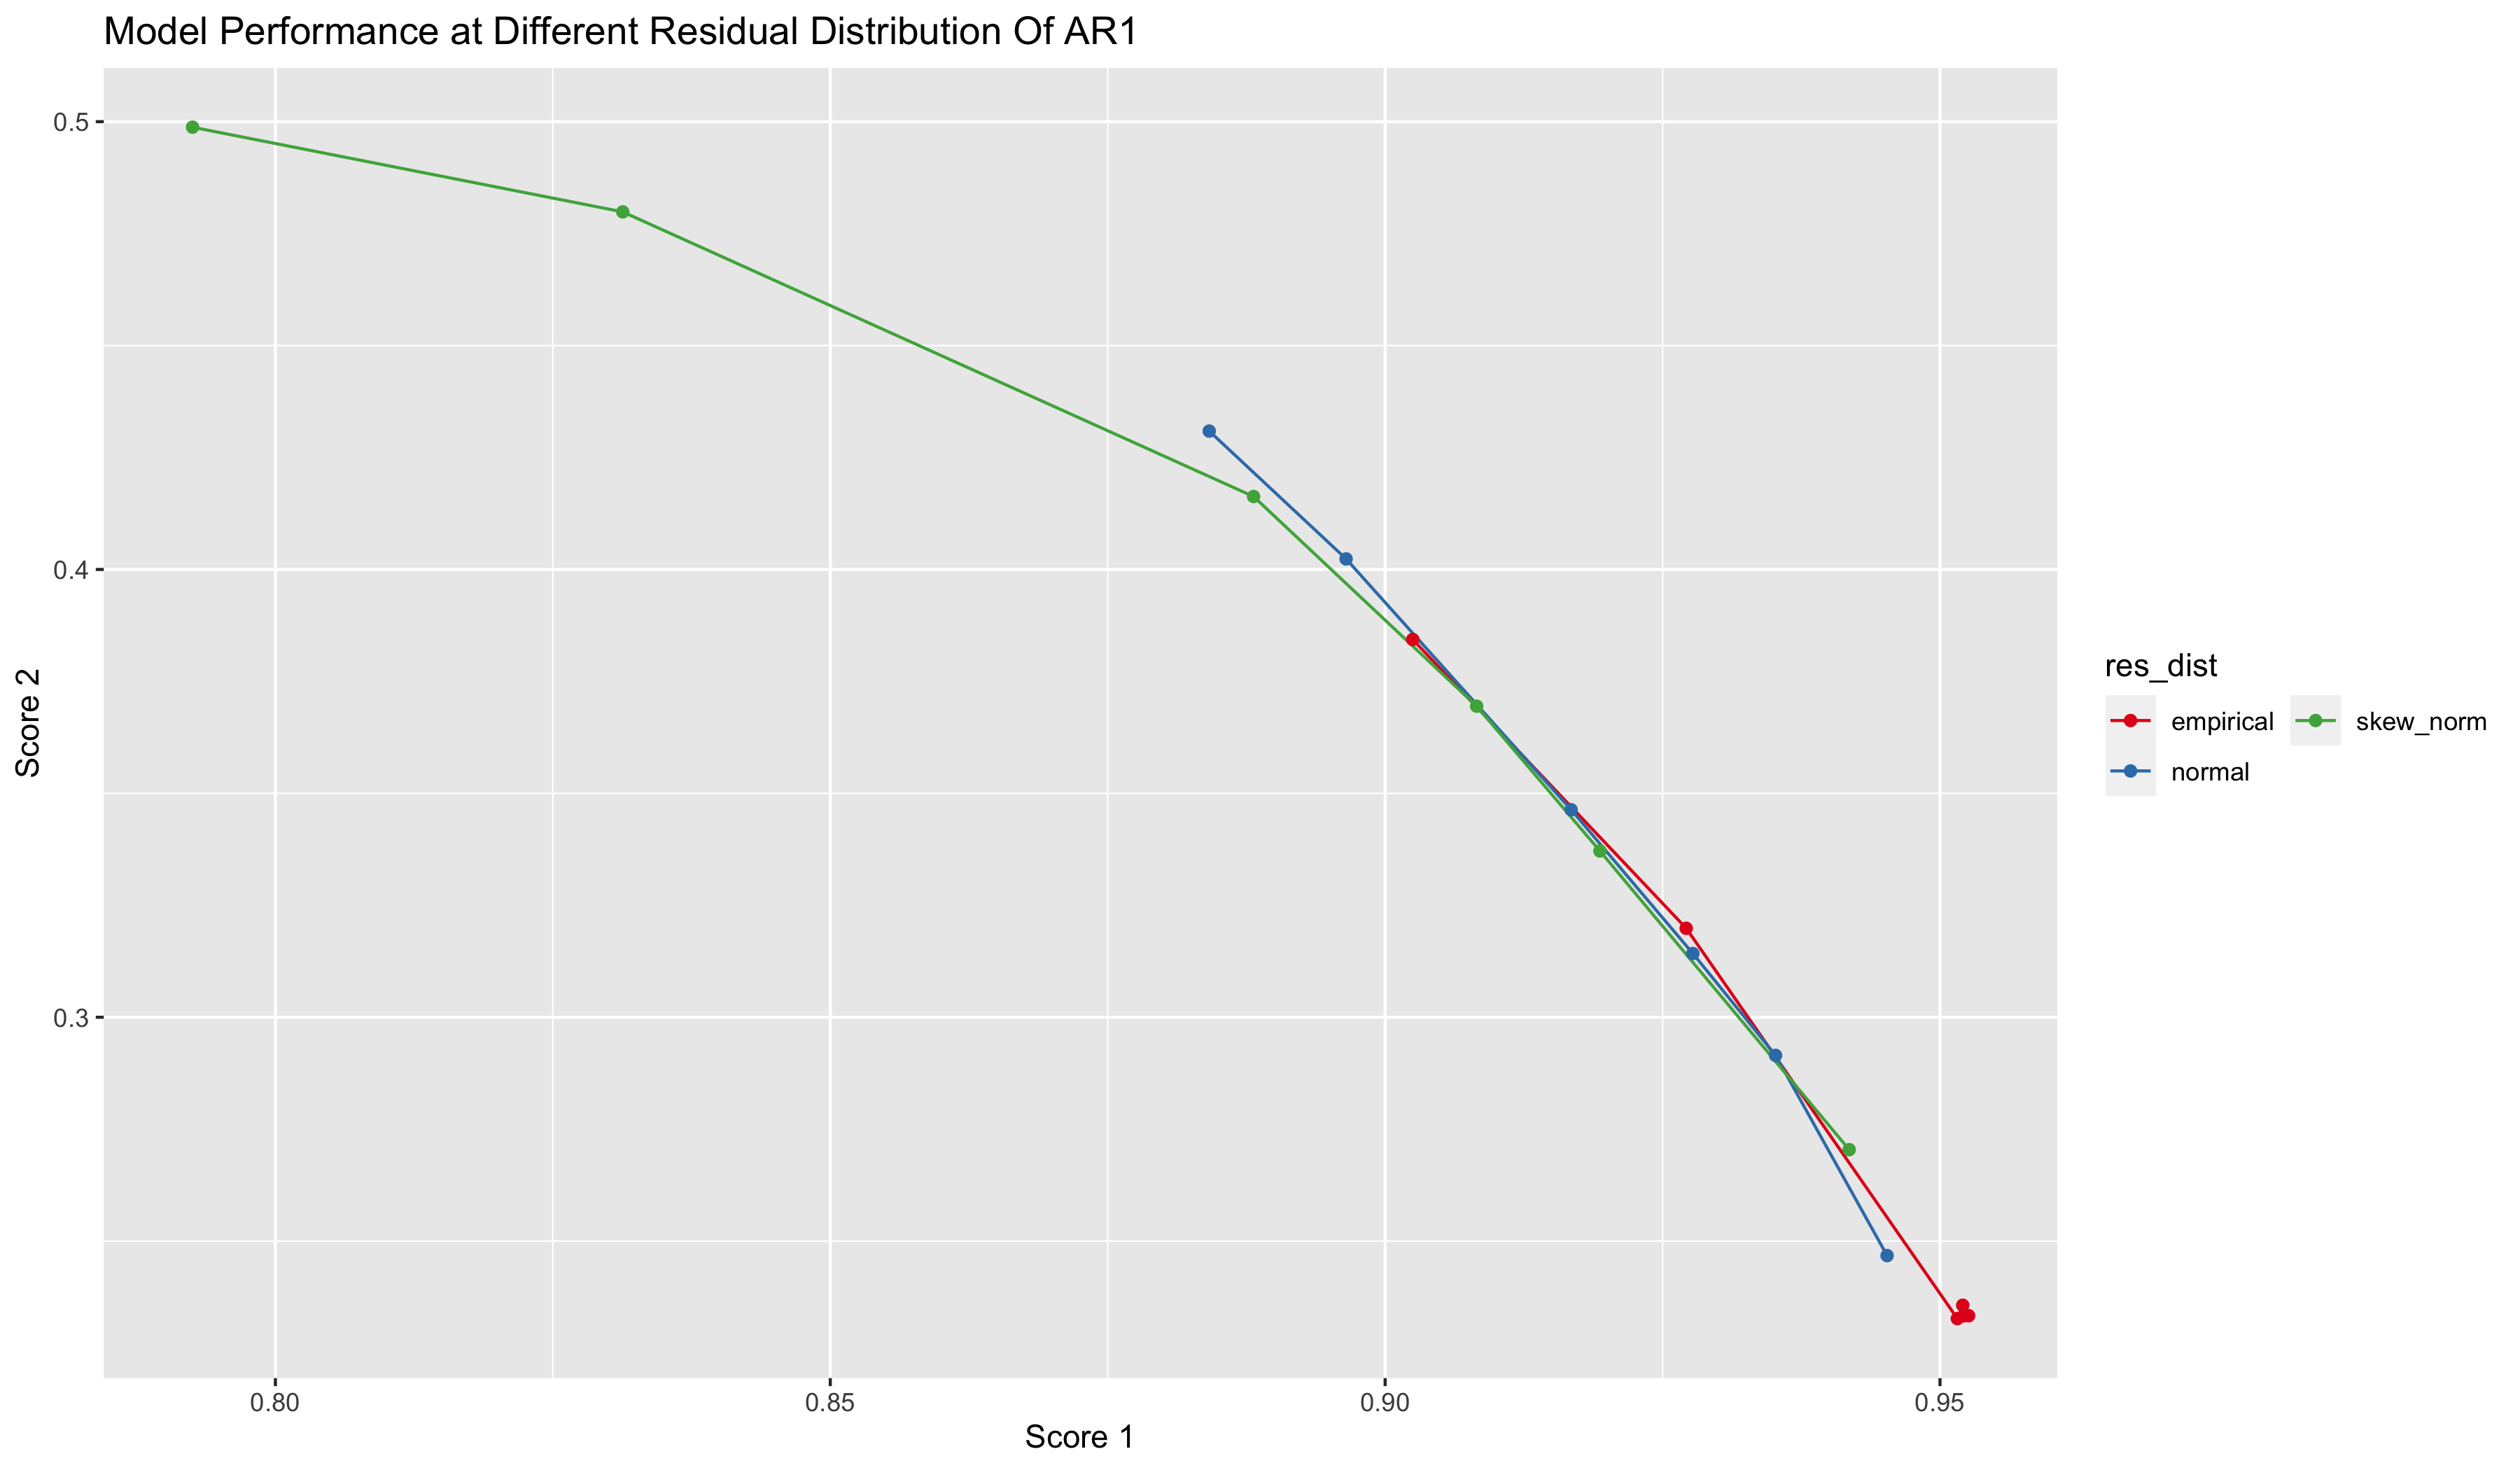
\includegraphics[width = 0.8\textwidth]{images/ModelPerformanceatDifferentResidualDistributionOfAR1.png}
    \label{fig:fig1.3.2}
\end{figure}

\begin{table}[htbp]
  \begin{center}
    \caption{Configuration and Result of AR1 Model with Different Residual Distribution Estimation}
    \label{tab:tab1.3.2}
    \begin{tabular}{l|l|*{4}{c}} \textbf{residual distribution} & \textbf{cut
      off prob} & \textbf{score 1} & \textbf{score 1 weight} & \textbf{score 2}
      & \textbf{score 2 weight} \\
      \hline
      Normal & 0.001 & 0.9452 & 42981 & 0.2468 & 59249\\
      Normal & 0.003 & 0.9352 & 46484 & 0.2915 & 59249\\
      Normal & 0.005 & 0.9277 & 47487 & 0.3142 & 59249\\
      Normal & 0.010 & 0.9168 & 48124 & 0.3463 & 59249\\
      Normal & 0.030 & 0.8965 & 50300 & 0.4024 & 59249\\
      Normal & 0.050 & 0.8841 & 52904 & 0.4309 & 59249\\
      Skew-normal & 0.001 & 0.9418 & 46008 & 0.2704 & 59249\\
      Skew-normal & 0.003 & 0.9194 & 47926 & 0.3371 & 59249\\
      Skew-normal & 0.005 & 0.9082 & 49578 & 0.3695 & 59249\\
      Skew-normal & 0.010 & 0.8881 & 51728 & 0.4163 & 59249\\
      Skew-normal & 0.030 & 0.8313 & 53154 & 0.4799 & 59249\\
      Skew-normal & 0.050 & 0.7925 & 54091 & 0.4988 & 59249\\
      Empirical & 0.001 & 0.9516 & 50437 & 0.2327 & 59249\\
      Empirical & 0.003 & 0.9526 & 50398 & 0.2334 & 59249\\
      Empirical & 0.005 & 0.9521 & 50434 & 0.2333 & 59249\\
      Empirical & 0.010 & 0.9520 & 50717 & 0.2357 & 59249\\
      Empirical & 0.030 & 0.9271 & 53533 & 0.3199 & 59249\\
      Empirical & 0.050 & 0.9025 & 55347 & 0.3844 & 59249\\
    \end{tabular}
  \end{center}
\end{table}

\begin{figure}[htbp]
    \caption{Trade-off Curves for AR1 with Different Outlier Detection Strategies}
    \centering
    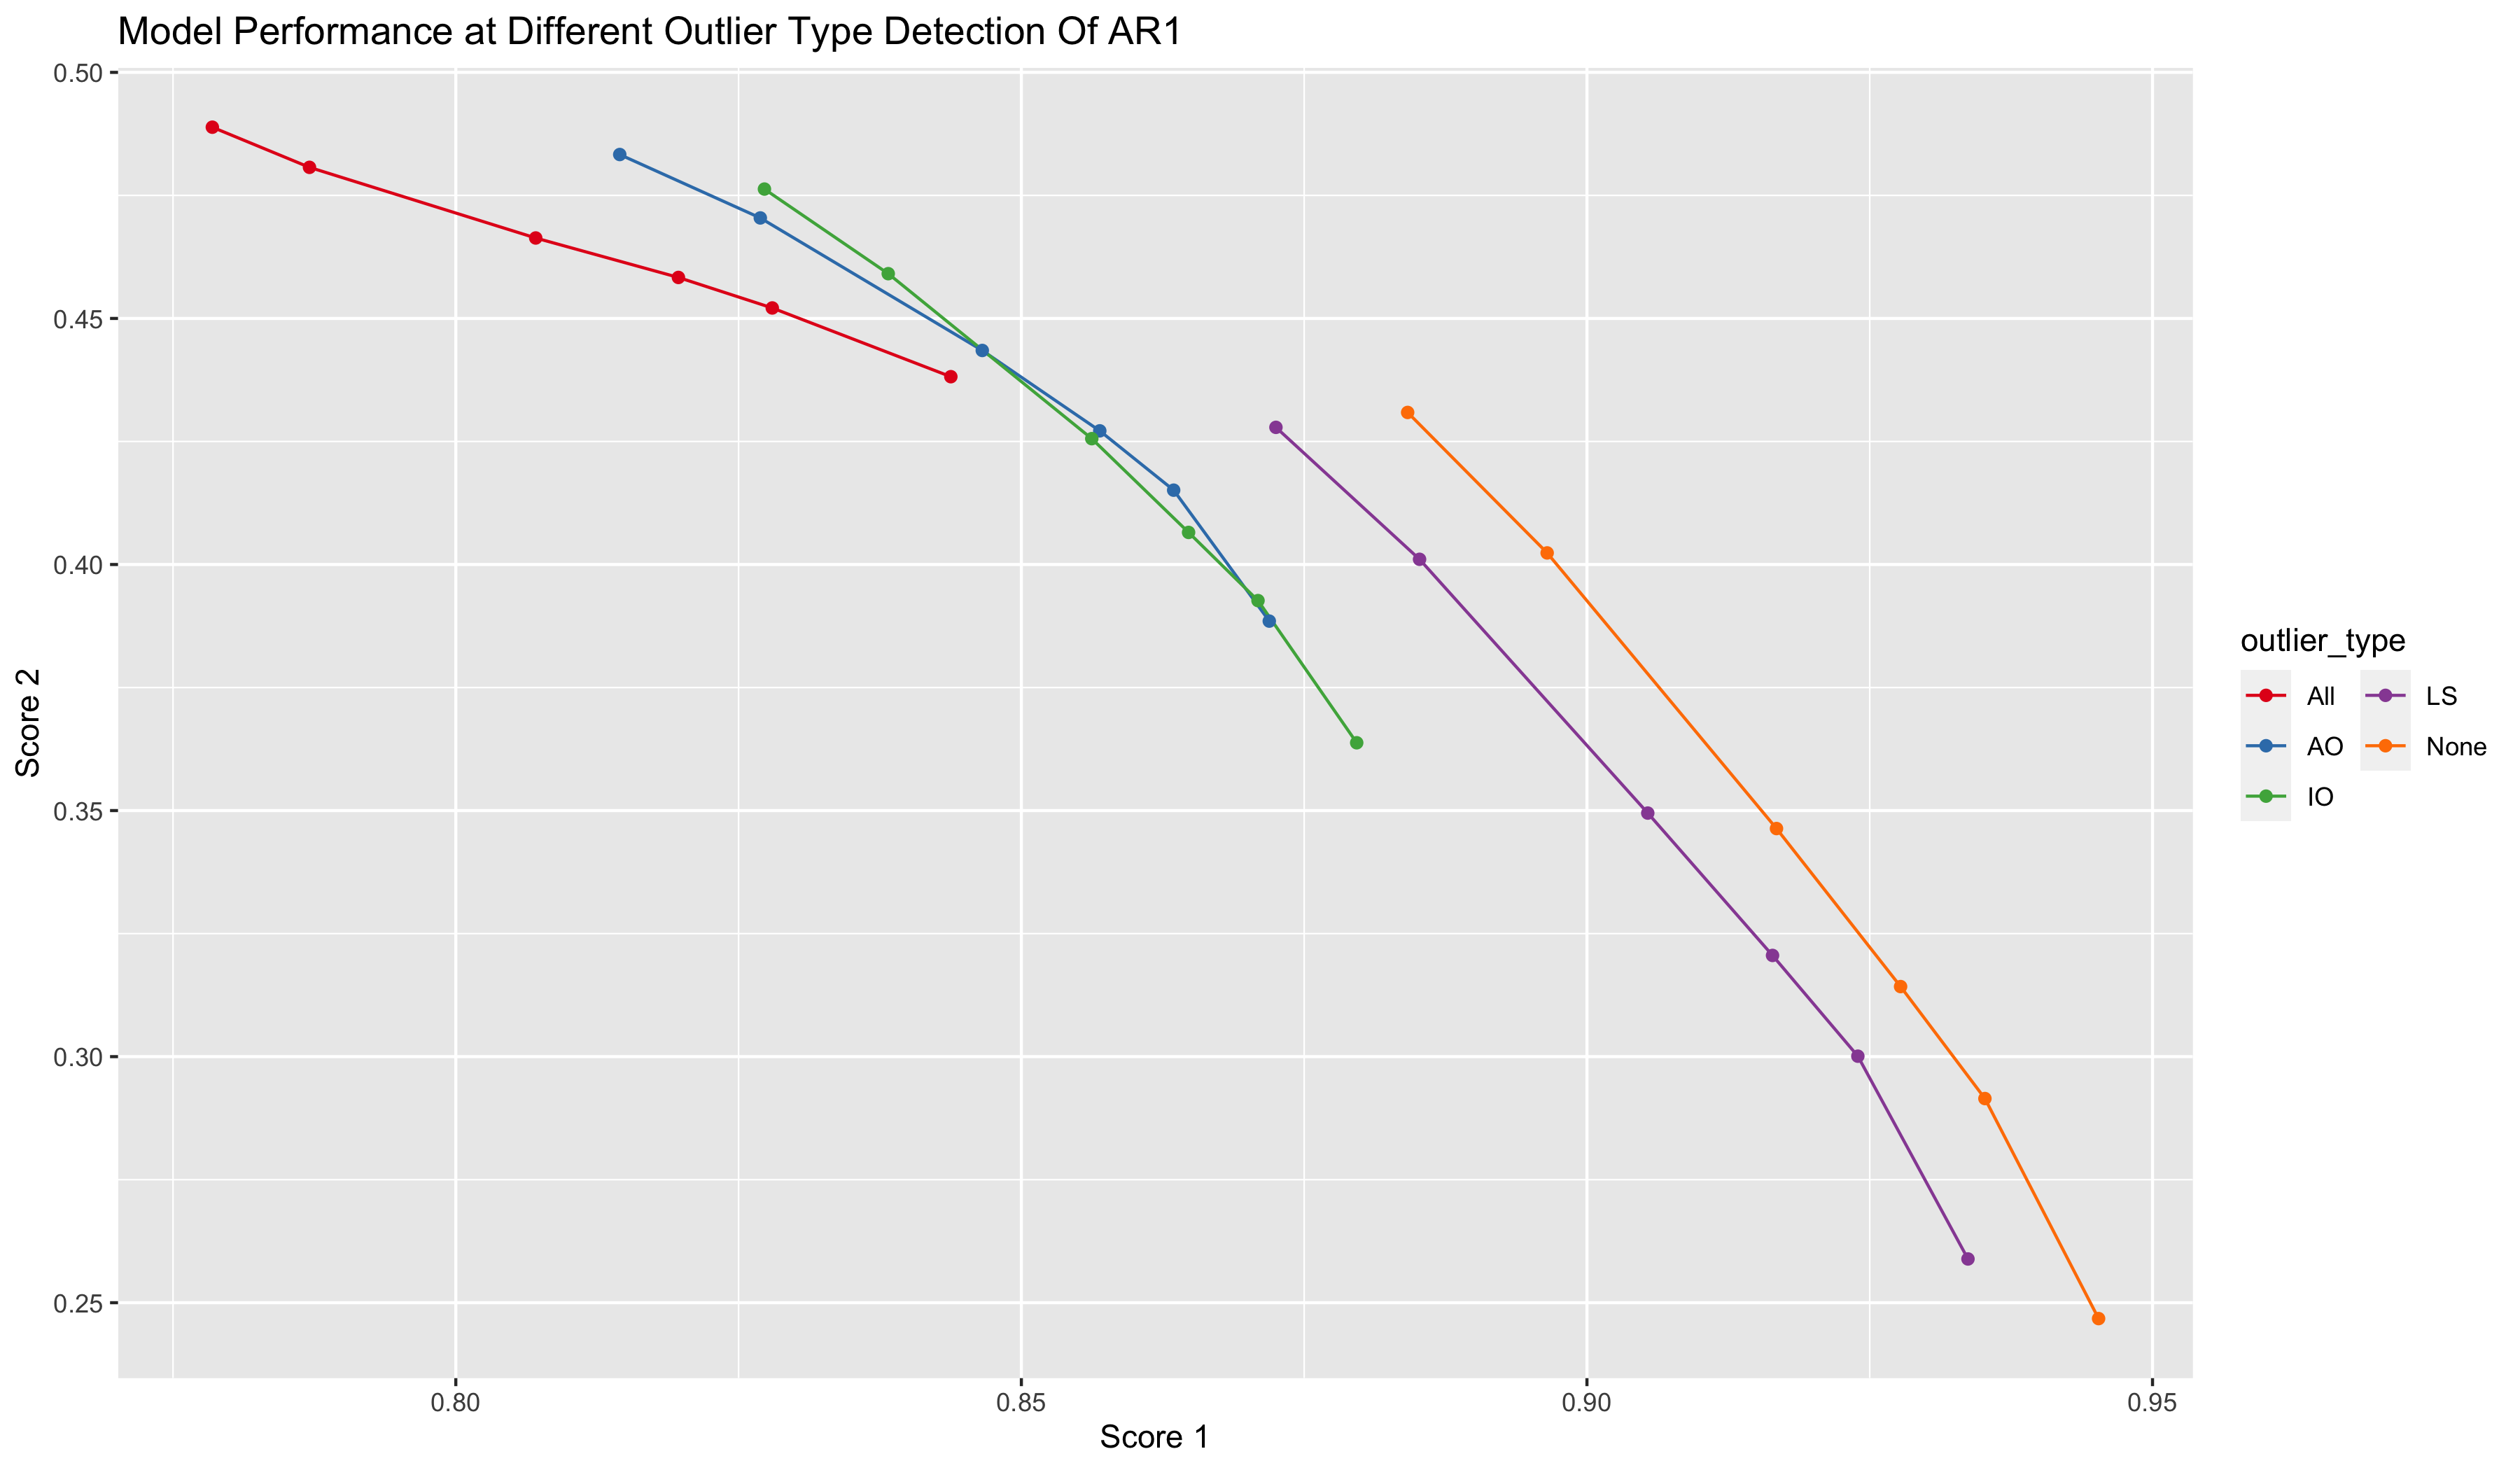
\includegraphics[width = 0.8\textwidth]{images/ModelPerformanceatDifferentOutlierTypeDetectionOfAR1.png}
    \label{fig:fig1.3.3}
\end{figure}

\begin{longtable}[htbp]{l|l|*{4}{c}}
    \caption{Configuration and Result of AR1 Model with Different Outlier Detection Strategies}
    \label{tab:tab1.3.3}\\
    \textbf{outlier type} & \textbf{cut off prob} & \textbf{score 1} &
    \textbf{score 1 weight} & \textbf{score 2} & \textbf{score 2 weight} \\
    \hline
    None & 0.001 & 0.9452 & 42981 & 0.2468 & 59249\\
    None & 0.003 & 0.9352 & 46484 & 0.2915 & 59249\\
    None & 0.005 & 0.9277 & 47487 & 0.3142 & 59249\\
    None & 0.010 & 0.9168 & 48124 & 0.3463 & 59249\\
    None & 0.030 & 0.8965 & 50300 & 0.4024 & 59249\\
    None & 0.050 & 0.8841 & 52904 & 0.4309 & 59249\\
    AO & 0.001 & 0.8719 & 48195 & 0.3885 & 59249\\
    AO & 0.003 & 0.8634 & 49576 & 0.4151 & 59249\\
    AO & 0.005 & 0.8569 & 49836 & 0.4272 & 59249\\
    AO & 0.010 & 0.8465 & 50288 & 0.4435 & 59249\\
    AO & 0.030 & 0.8269 & 52421 & 0.4704 & 59249\\
    AO & 0.050 & 0.8145 & 50288 & 0.4408 & 59249\\
    IO & 0.001 & 0.8796 & 47127 & 0.3638 & 59249\\
    IO & 0.003 & 0.8709 & 48489 & 0.3927 & 59249\\
    IO & 0.005 & 0.8648 & 48810 & 0.4065 & 59249\\
    IO & 0.010 & 0.8562 & 49834 & 0.4256 & 59249\\
    IO & 0.030 & 0.8382 & 52346 & 0.4591 & 59249\\
    IO & 0.050 & 0.8273 & 54894 & 0.4763 & 59249\\
    LS & 0.001 & 0.9337 & 42735 & 0.2589 & 59249\\
    LS & 0.003 & 0.9239 & 46469 & 0.3001 & 59249\\
    LS & 0.005 & 0.9164 & 47456 & 0.3206 & 59249\\
    LS & 0.010 & 0.9054 & 48360 & 0.3495 & 59249\\
    LS & 0.030 & 0.8852 & 50802 & 0.4011 & 59249\\
    LS & 0.050 & 0.8725 & 53029 & 0.4279 & 59249\\
    All & 0.001 & 0.8438 & 50238 & 0.4382 & 59249\\
    All & 0.003 & 0.8280 & 50563 & 0.4521 & 59249\\
    All & 0.005 & 0.8197 & 50671 & 0.4583 & 59249\\
    All & 0.010 & 0.8071 & 50820 & 0.4663 & 59249\\
    All & 0.030 & 0.7871 & 52401 & 0.4807 & 59249\\
    All & 0.050 & 0.7785 & 54721 & 0.4889 & 59249\\
\end{longtable}

\begin{figure}[htbp]
    \caption{Trade-off Curves for Different Markov Models}
    \centering
    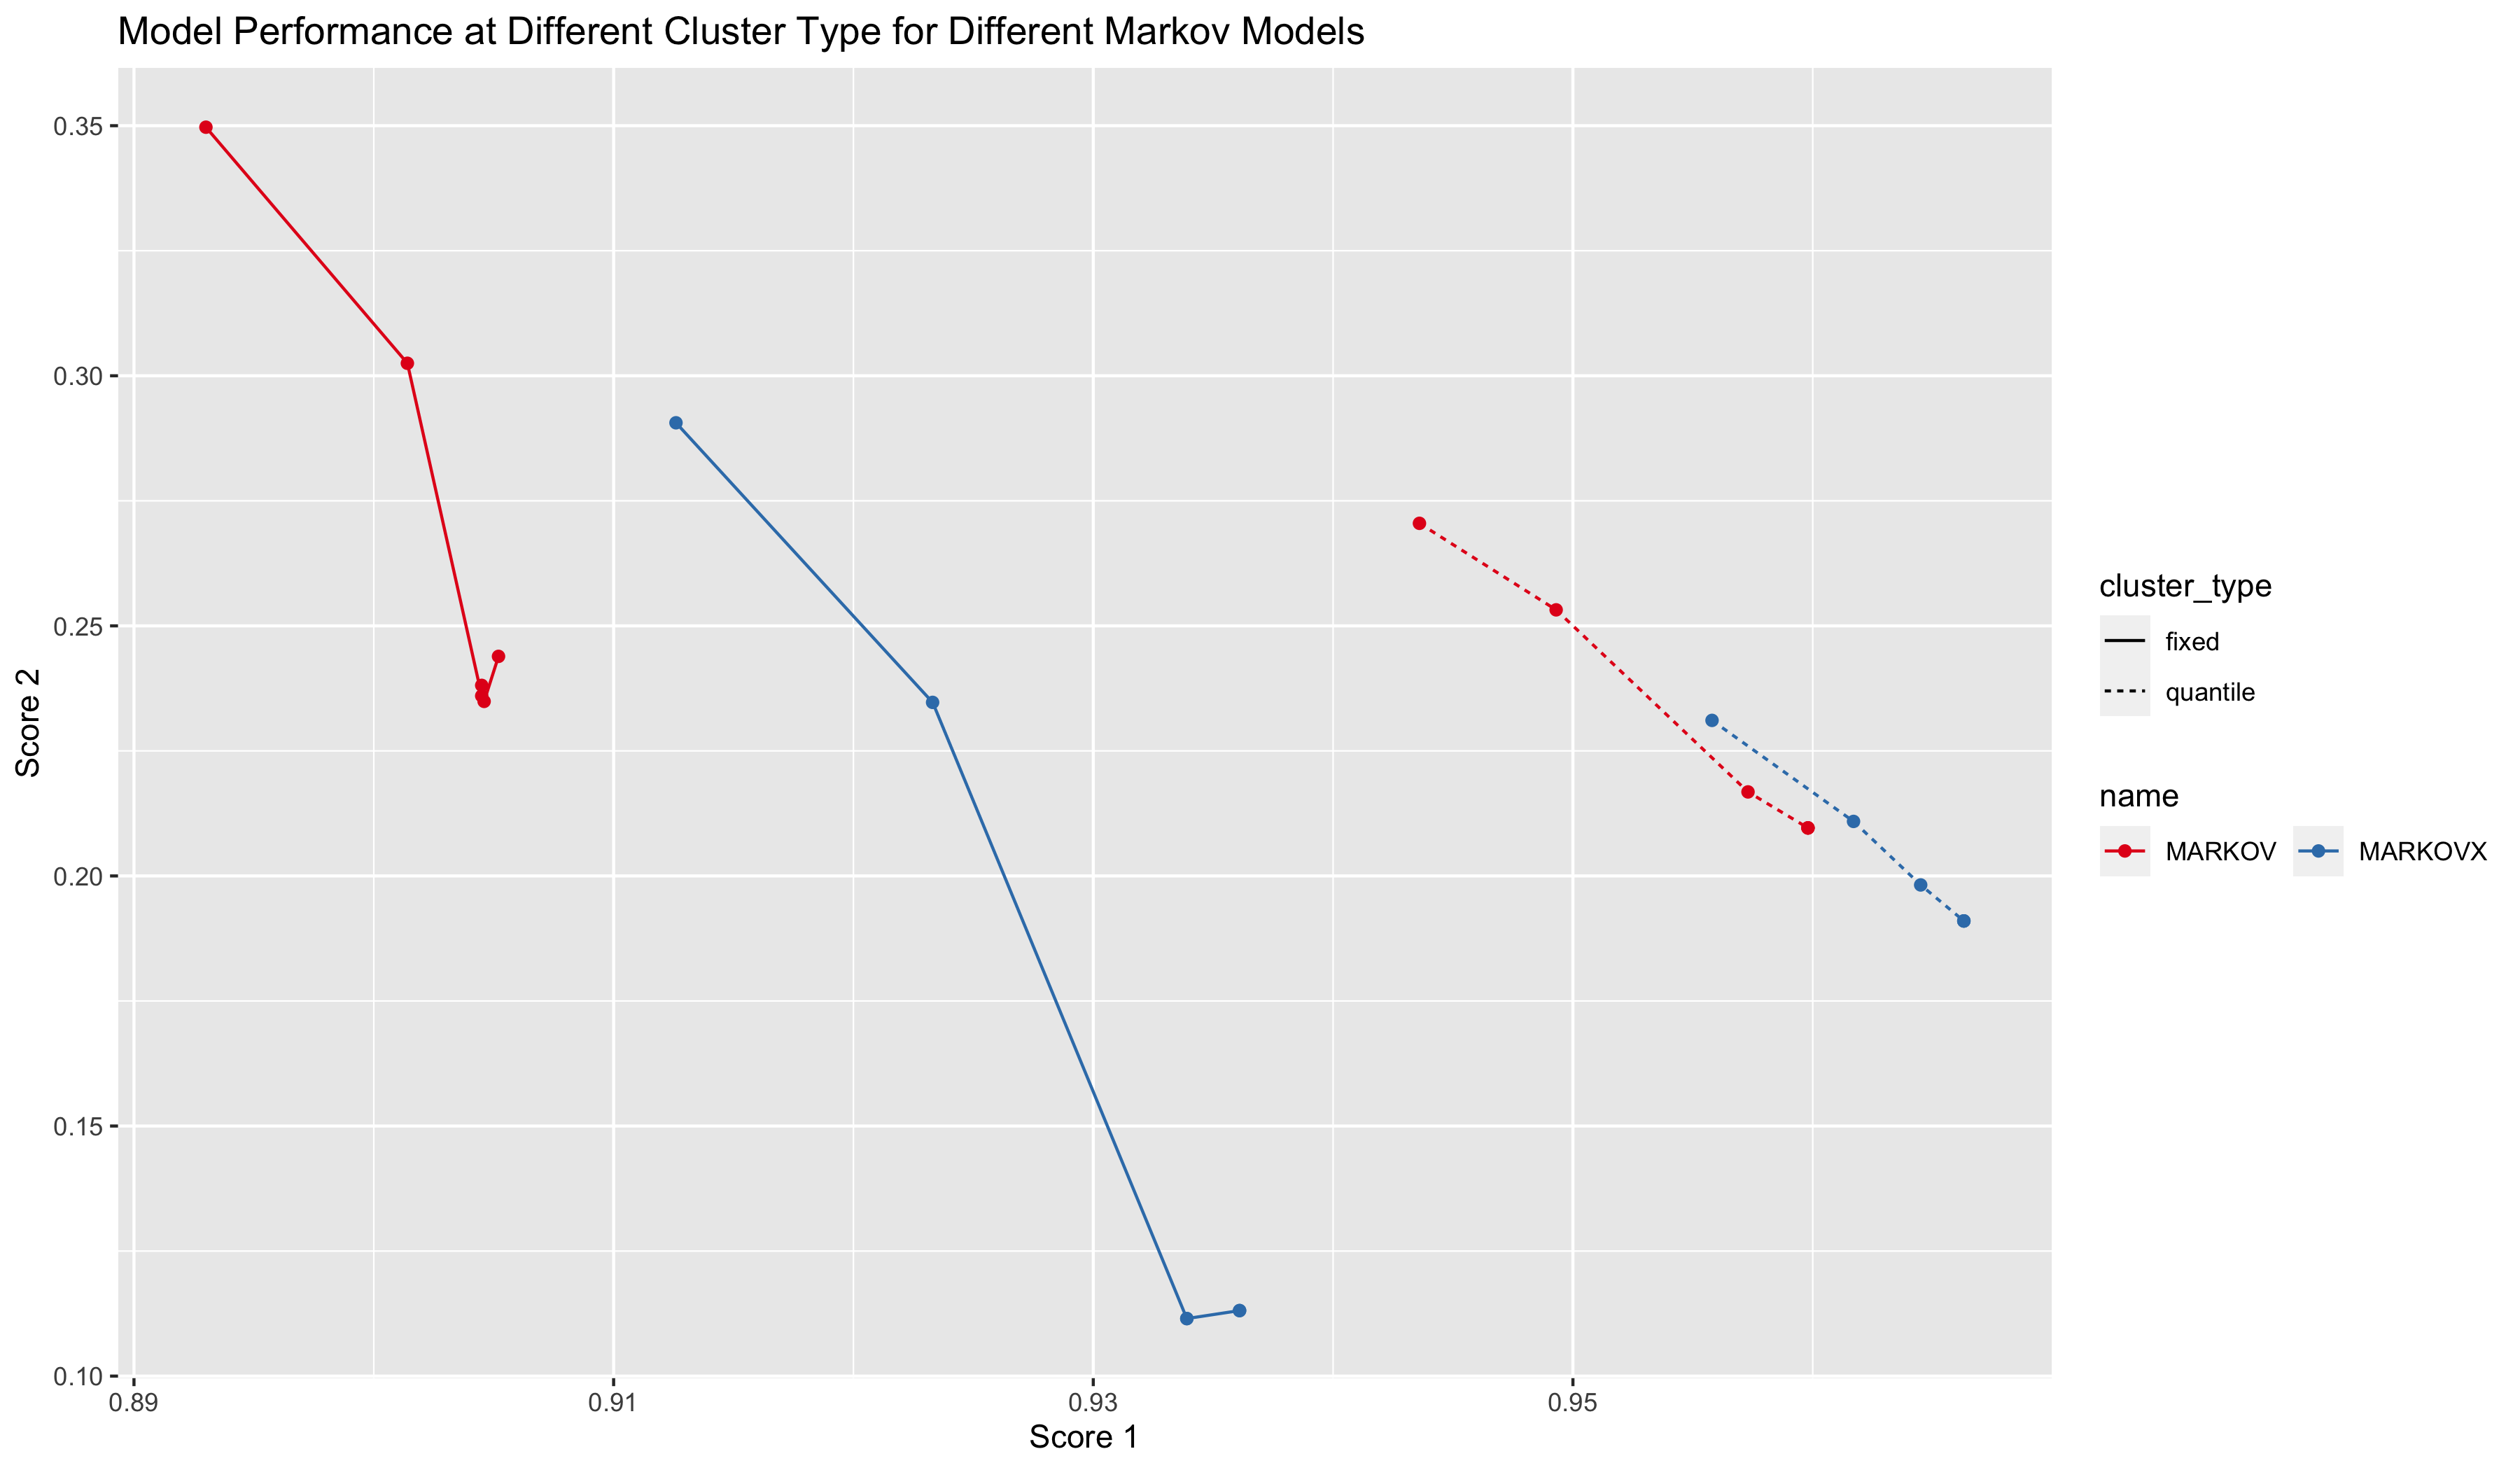
\includegraphics[width = 0.8\textwidth]{images/ModelPerformanceatDifferentClusterTypeforDifferentMarkovModels.png}
    \label{fig:fig1.3.4}
\end{figure}

\begin{longtable}[htbp]{l|l|l|*{4}{c}}
    \caption{Configuration and Result of Markov Models with Different Partitioning Methods}
    \label{tab:tab1.3.4}\\
    \textbf{model name} & \textbf{partitioning type} & \textbf{cut off prob} &
    \textbf{score 1} & \textbf{score 1 weight} & \textbf{score 2} &
    \textbf{score 2 weight} \\
    \hline
    MARKOV & fixed & 0.001 & 0.9046 & 29990 & 0.2349 & 59249\\
    MARKOV & fixed & 0.003 & 0.9045 & 30082 & 0.2360 & 59249\\
    MARKOV & fixed & 0.005 & 0.9045 & 30195 & 0.2381 & 59249\\
    MARKOV & fixed & 0.010 & 0.9052 & 31233 & 0.2439 & 59249\\
    MARKOV & fixed & 0.030 & 0.9014 & 37994 & 0.3025 & 59249\\
    MARKOV & fixed & 0.050 & 0.8930 & 41058 & 0.3497 & 59249\\
    MARKOVX & fixed & 0.001 & 0.9339 & 16849 & 0.1115 & 59249\\
    MARKOVX & fixed & 0.003 & 0.9339 & 16849 & 0.1115 & 59249\\
    MARKOVX & fixed & 0.005 & 0.9361 & 17443 & 0.1131 & 59249\\
    MARKOVX & fixed & 0.010 & 0.9361 & 17443 & 0.1131 & 59249\\
    MARKOVX & fixed & 0.030 & 0.9233 & 32287 & 0.2347 & 59249\\
    MARKOVX & fixed & 0.050 & 0.9126 & 36591 & 0.2906 & 59249\\
    MARKOV & quantile & 0.001 & 0.9598 & 56899 & 0.2096 & 59249\\
    MARKOV & quantile & 0.003 & 0.9598 & 56899 & 0.2096 & 59249\\
    MARKOV & quantile & 0.005 & 0.9598 & 56899 & 0.2096 & 59249\\
    MARKOV & quantile & 0.010 & 0.9573 & 56899 & 0.2168 & 59249\\
    MARKOV & quantile & 0.030 & 0.9493 & 56918 & 0.2532 & 59249\\
    MARKOV & quantile & 0.050 & 0.9436 & 56918 & 0.2705 & 59249\\
    MARKOVX & quantile & 0.001 & 0.9663 & 56511 & 0.191 & 59249\\
    MARKOVX & quantile & 0.003 & 0.9663 & 56511 & 0.191 & 59249\\
    MARKOVX & quantile & 0.005 & 0.9663 & 56511 & 0.191 & 59249\\
    MARKOVX & quantile & 0.010 & 0.9645 & 56650 & 0.1982 & 59249\\
    MARKOVX & quantile & 0.030 & 0.9617 & 56650 & 0.2109 & 59249\\
    MARKOVX & quantile & 0.050 & 0.9558 & 56650 & 0.2311 & 59249\\

\end{longtable}

\begin{figure}[htbp]
    \caption{Trade-off Curves for Different States for Markov Models}
    \centering
    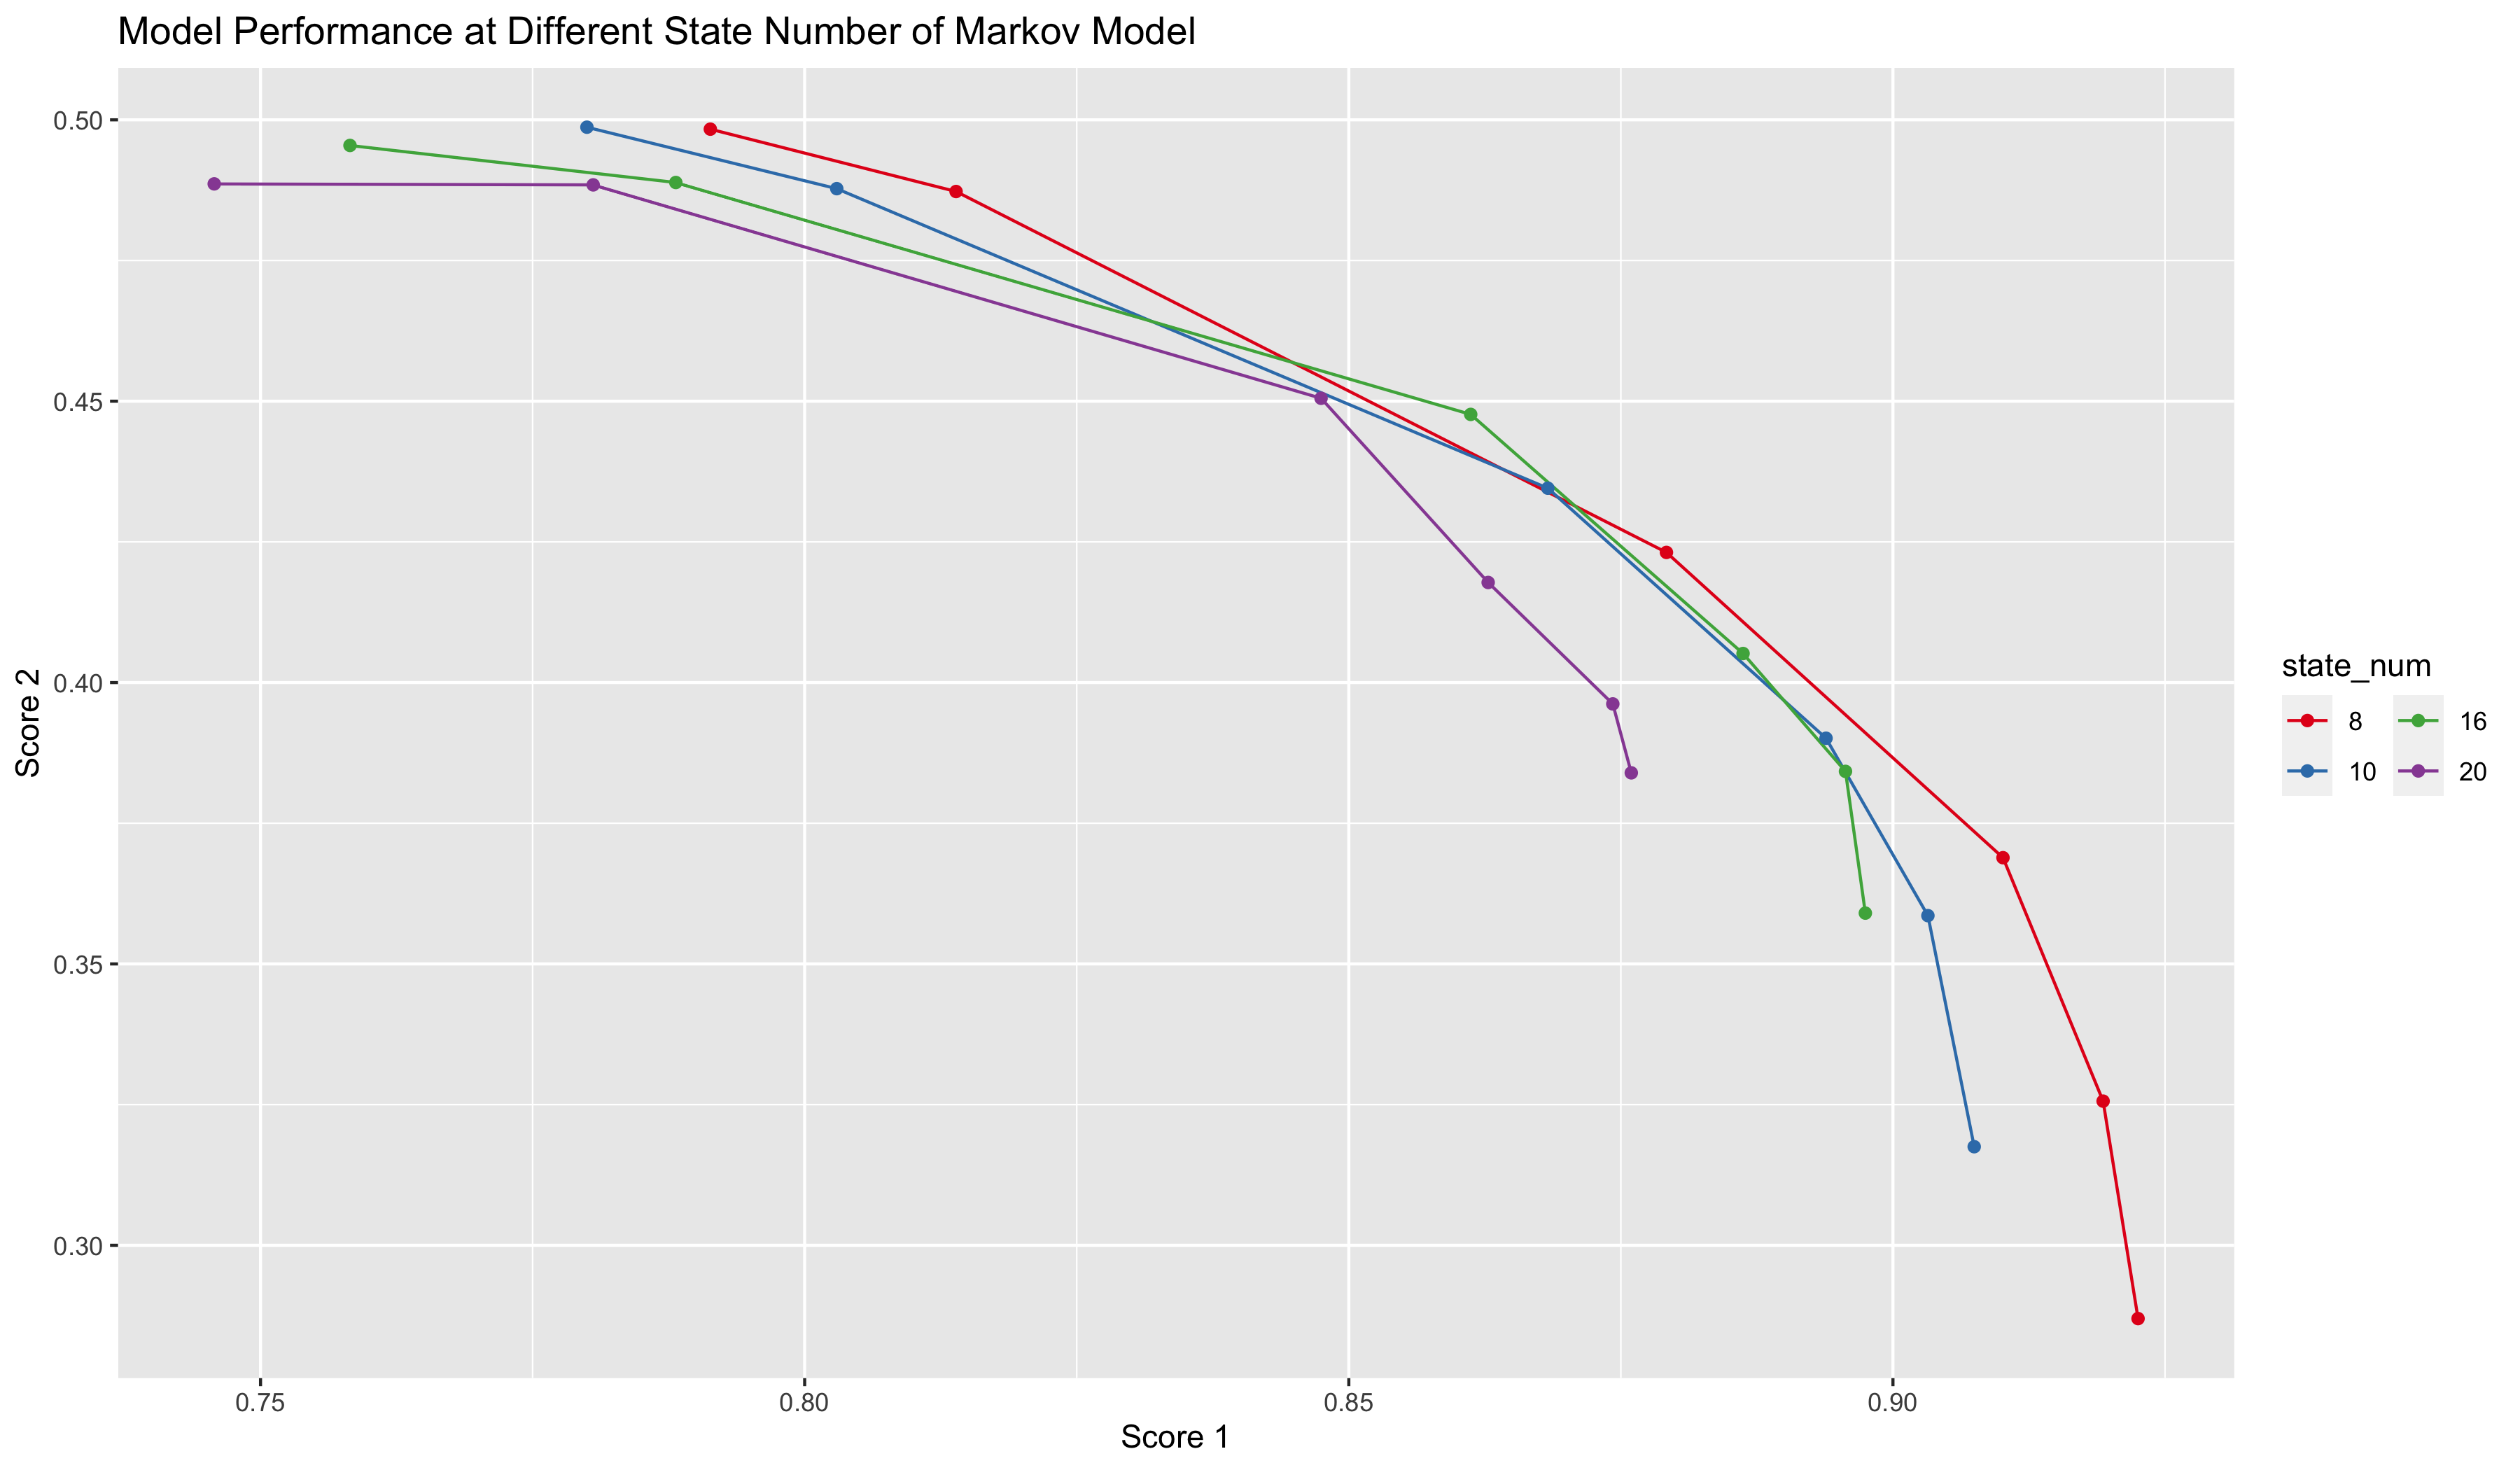
\includegraphics[width = 0.8\textwidth]{images/ModelPerformanceatDifferentStateNumberofMarkovModel.png}
    \label{fig:fig1.3.5}
\end{figure}

\begin{longtable}[htbp]{l|l|*{4}{c}}
    \caption{Configuration and Result of Markov Model with Different Number of States}
    \label{tab:tab1.3.5}\\
    \textbf{state num} & \textbf{cut off prob} & \textbf{score 1} &
    \textbf{score 1 weight} & \textbf{score 2} & \textbf{score 2 weight} \\
    \hline
    8 & 0.001 & 0.9225 & 36075 & 0.2870 & 59249\\
    8 & 0.003 & 0.9193 & 40043 & 0.3256 & 59249\\
    8 & 0.005 & 0.9101 & 41985 & 0.3689 & 59249\\
    8 & 0.010 & 0.8792 & 45459 & 0.4231 & 59249\\
    8 & 0.030 & 0.8139 & 49858 & 0.4873 & 59249\\
    8 & 0.050 & 0.7913 & 51268 & 0.4983 & 59249\\
    10 & 0.001 & 0.9075 & 39391 & 0.4306 & 59249\\
    10 & 0.003 & 0.9032 & 42650 & 0.4306 & 59249\\
    10 & 0.005 & 0.8939 & 44164 & 0.4306 & 59249\\
    10 & 0.010 & 0.8683 & 46253 & 0.4306 & 59249\\
    10 & 0.030 & 0.8029 & 50804 & 0.4306 & 59249\\
    10 & 0.050 & 0.7800 & 51898 & 0.4306 & 59249\\
    16 & 0.001 & 0.8975 & 42678 & 0.4282 & 59249\\
    16 & 0.003 & 0.8956 & 45218 & 0.4282 & 59249\\
    16 & 0.005 & 0.8862 & 45828 & 0.4282 & 59249\\
    16 & 0.010 & 0.8612 & 47846 & 0.4282 & 59249\\
    16 & 0.030 & 0.7882 & 51331 & 0.4282 & 59249\\
    16 & 0.050 & 0.7582 & 52399 & 0.4282 & 59249\\
    20 & 0.001 & 0.8760 & 45960 & 0.3840 & 59249\\
    20 & 0.003 & 0.8743 & 46770 & 0.3962 & 59249\\
    20 & 0.005 & 0.8628 & 47254 & 0.4178 & 59249\\
    20 & 0.010 & 0.8475 & 48876 & 0.4505 & 59249\\
    20 & 0.030 & 0.7806 & 52390 & 0.4884 & 59249\\
    20 & 0.050 & 0.7457 & 52809 & 0.4886 & 59249\\
\end{longtable}

\begin{figure}[htbp]
    \caption{Trade-off Curves for Different Multivariate Models}
    \centering
    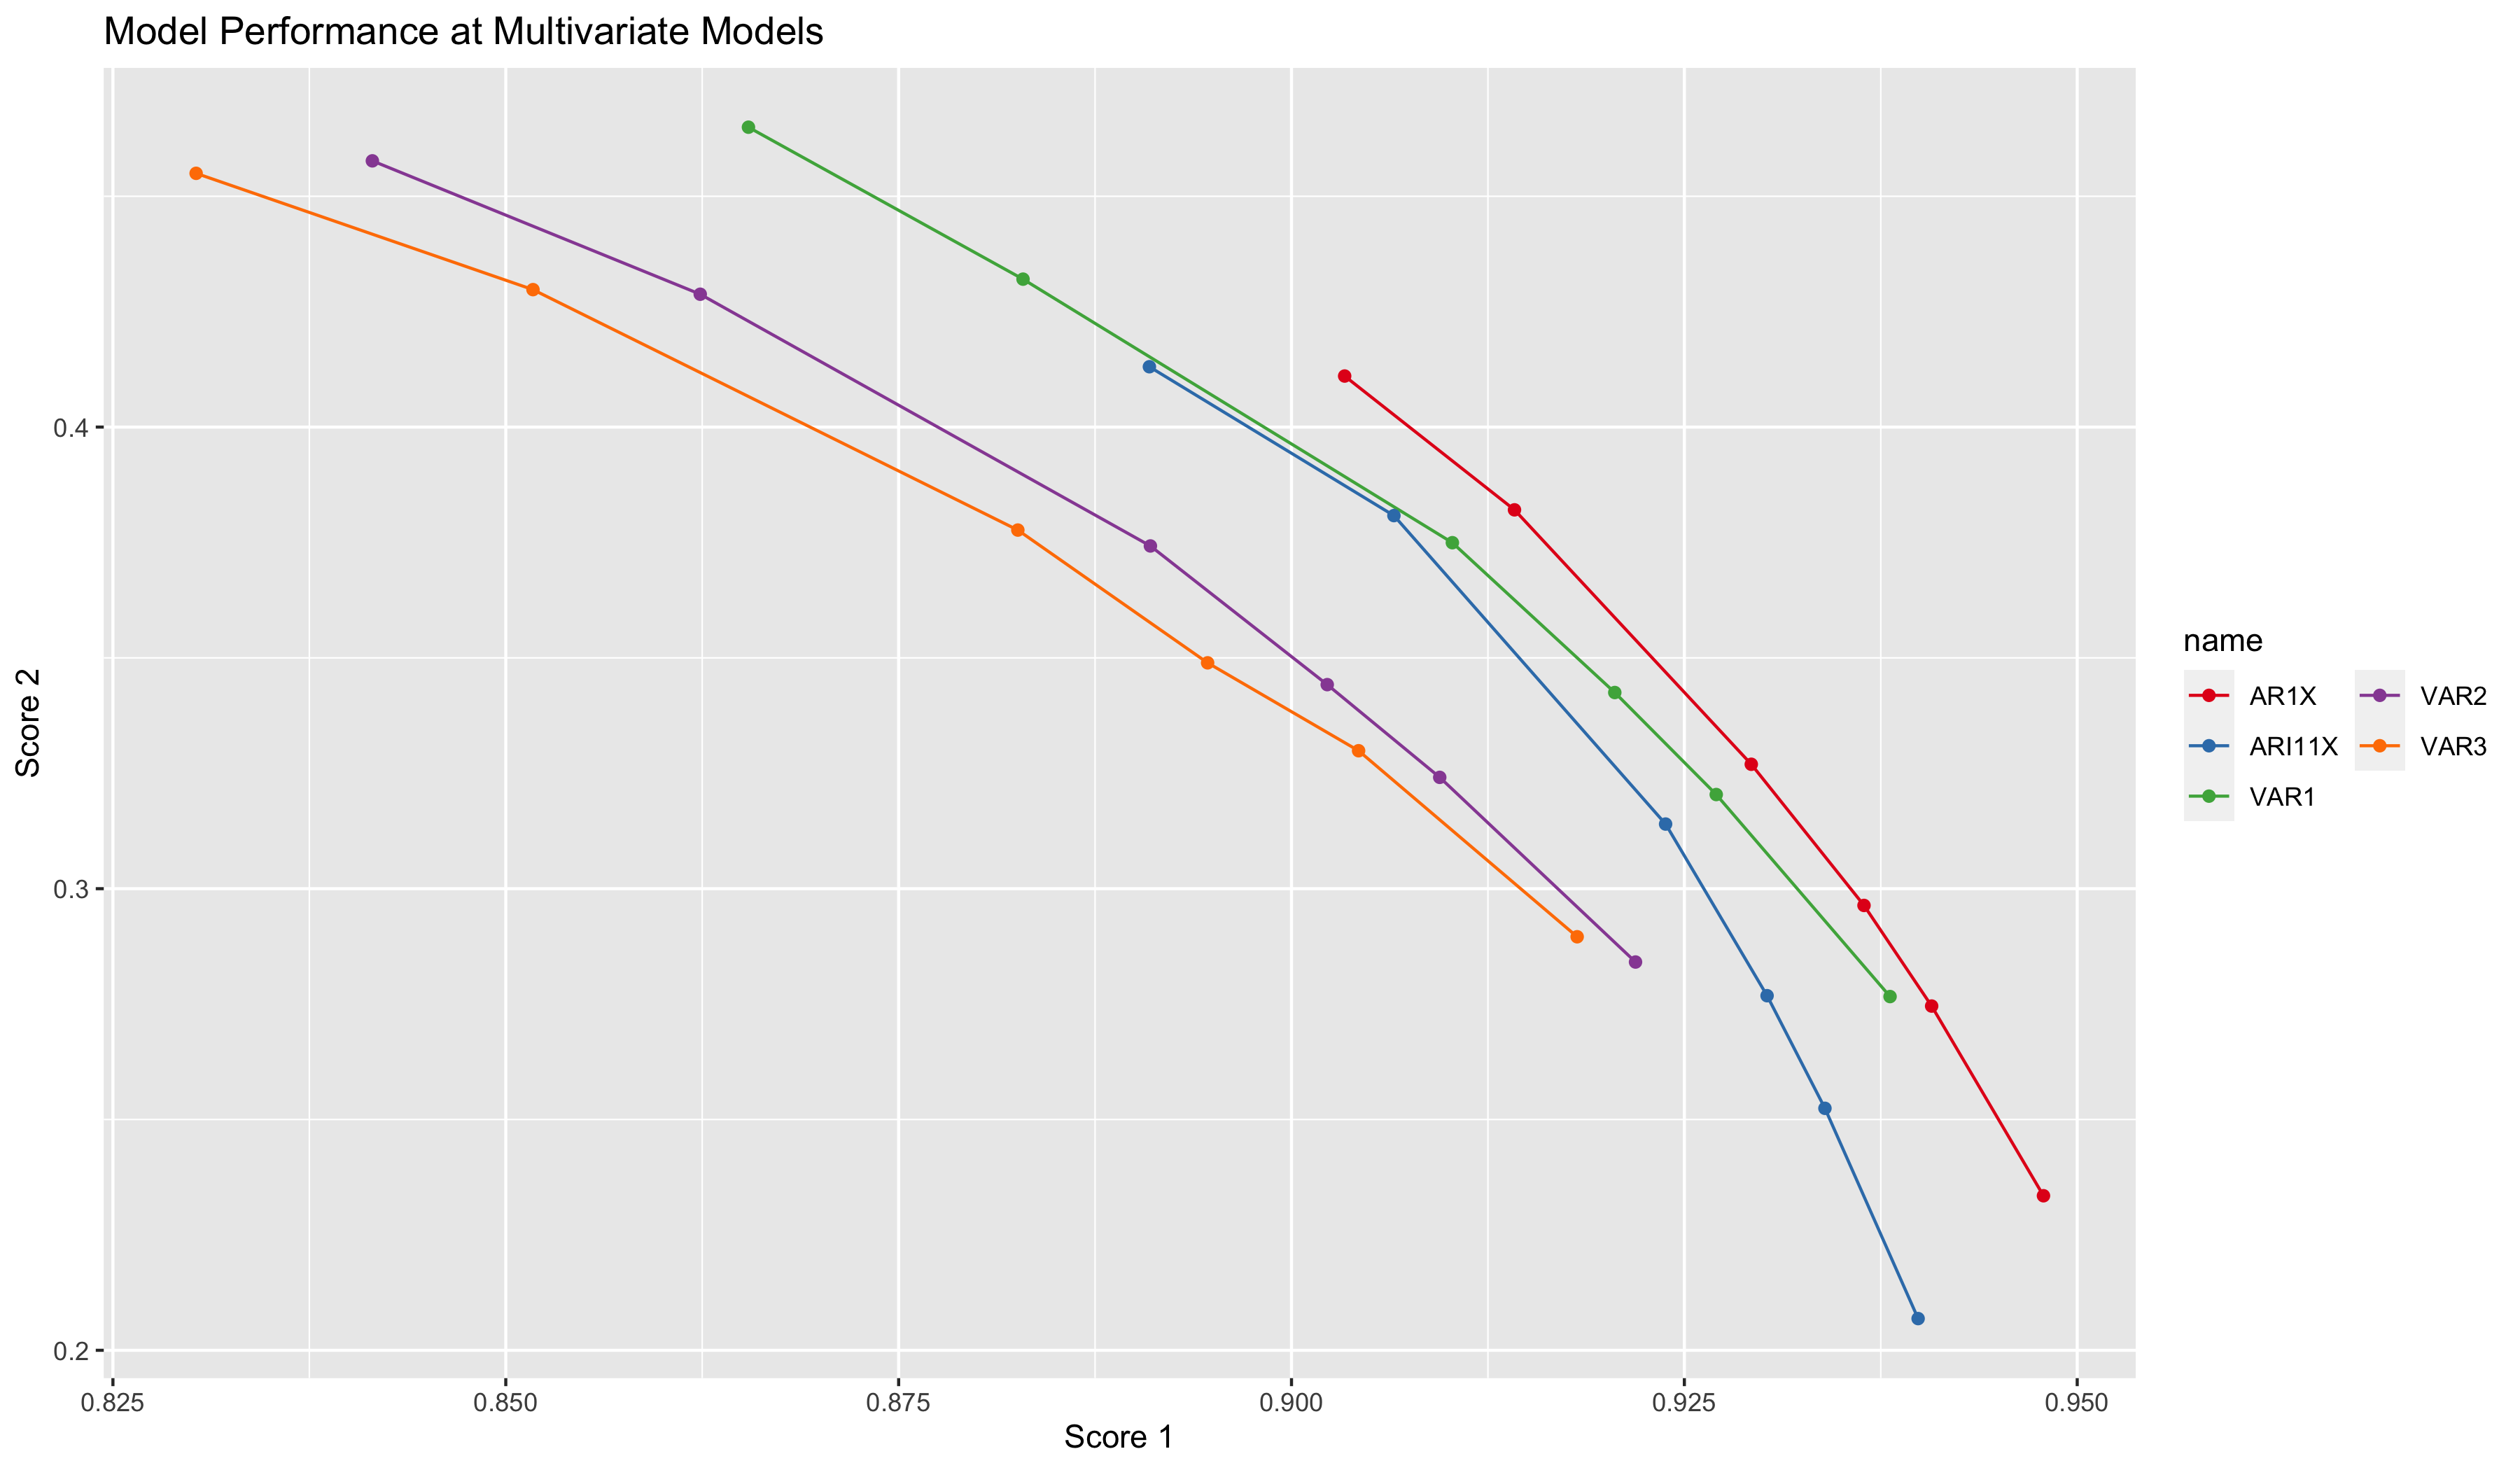
\includegraphics[width = 0.8\textwidth]{images/ModelPerformanceatMultivariateModels.png}
    \label{fig:fig1.3.6}
\end{figure}

\begin{table}[htbp]
  \begin{center}
    \caption{Configuration and Result of AR1 Model with Different Outlier Detections}
    \label{tab:tab1.3.6}
    \begin{tabular}{l|l|*{4}{c}} \textbf{model name} & \textbf{cut off prob} &
      \textbf{score 1} & \textbf{score 1 weight} & \textbf{score 2} &
      \textbf{score 2 weight} \\
      \hline
      AR1X & 0.001 & 0.9479 & 41306 & 0.2335 & 59249\\
      AR1X & 0.003 & 0.9407 & 43602 & 0.2746 & 59249\\
      AR1X & 0.005 & 0.9364 & 44299 & 0.2964 & 59249\\
      AR1X & 0.010 & 0.9293 & 45094 & 0.3270 & 59249\\
      AR1X & 0.030 & 0.9142 & 47570 & 0.3821 & 59249\\
      AR1X & 0.050 & 0.9034 & 50374 & 0.4111 & 59249\\
      ARI11X & 0.001 & 0.9399 & 38470 & 0.2069 & 59249\\
      ARI11X & 0.003 & 0.9339 & 42132 & 0.2524 & 59249\\
      ARI11X & 0.005 & 0.9303 & 43794 & 0.2768 & 59249\\
      ARI11X & 0.010 & 0.9238 & 45778 & 0.3140 & 59249\\
      ARI11X & 0.030 & 0.9065 & 48501 & 0.3808 & 59249\\
      ARI11X & 0.050 & 0.8910 & 49852 & 0.4131 & 59249\\
      VAR1 & 0.001 & 0.9381 & 44419 & 0.2766 & 59249\\
      VAR1 & 0.003 & 0.9270 & 46114 & 0.3204 & 59249\\
      VAR1 & 0.005 & 0.9206 & 46533 & 0.3425 & 59249\\
      VAR1 & 0.010 & 0.9102 & 47837 & 0.3750 & 59249\\
      VAR1 & 0.030 & 0.8829 & 51860 & 0.4320 & 59249\\
      VAR1 & 0.050 & 0.8654 & 53962 & 0.4650 & 59249\\
      VAR2 & 0.001 & 0.9219 & 44733 & 0.2841 & 59249\\
      VAR2 & 0.003 & 0.9094 & 46551 & 0.3241 & 59249\\
      VAR2 & 0.005 & 0.9023 & 47142 & 0.3442 & 59249\\
      VAR2 & 0.010 & 0.8910 & 48459 & 0.3742 & 59249\\
      VAR2 & 0.030 & 0.8624 & 52483 & 0.4288 & 59249\\
      VAR2 & 0.050 & 0.8415 & 54281 & 0.4577 & 59249\\
      VAR3 & 0.001 & 0.9181 & 44719 & 0.2895 & 59249\\
      VAR3 & 0.003 & 0.9043 & 46798 & 0.3299 & 59249\\
      VAR3 & 0.005 & 0.8947 & 47713 & 0.3489 & 59249\\
      VAR3 & 0.010 & 0.8826 & 48861 & 0.3777 & 59249\\
      VAR3 & 0.030 & 0.8517 & 52978 & 0.4298 & 59249\\
      VAR3 & 0.050 & 0.8303 & 53852 & 0.4550 & 59249\\
    \end{tabular}
  \end{center}
\end{table}

\begin{figure}[htbp]
    \caption{Trade-off Curves for Different Neural Network Models}
    \centering
    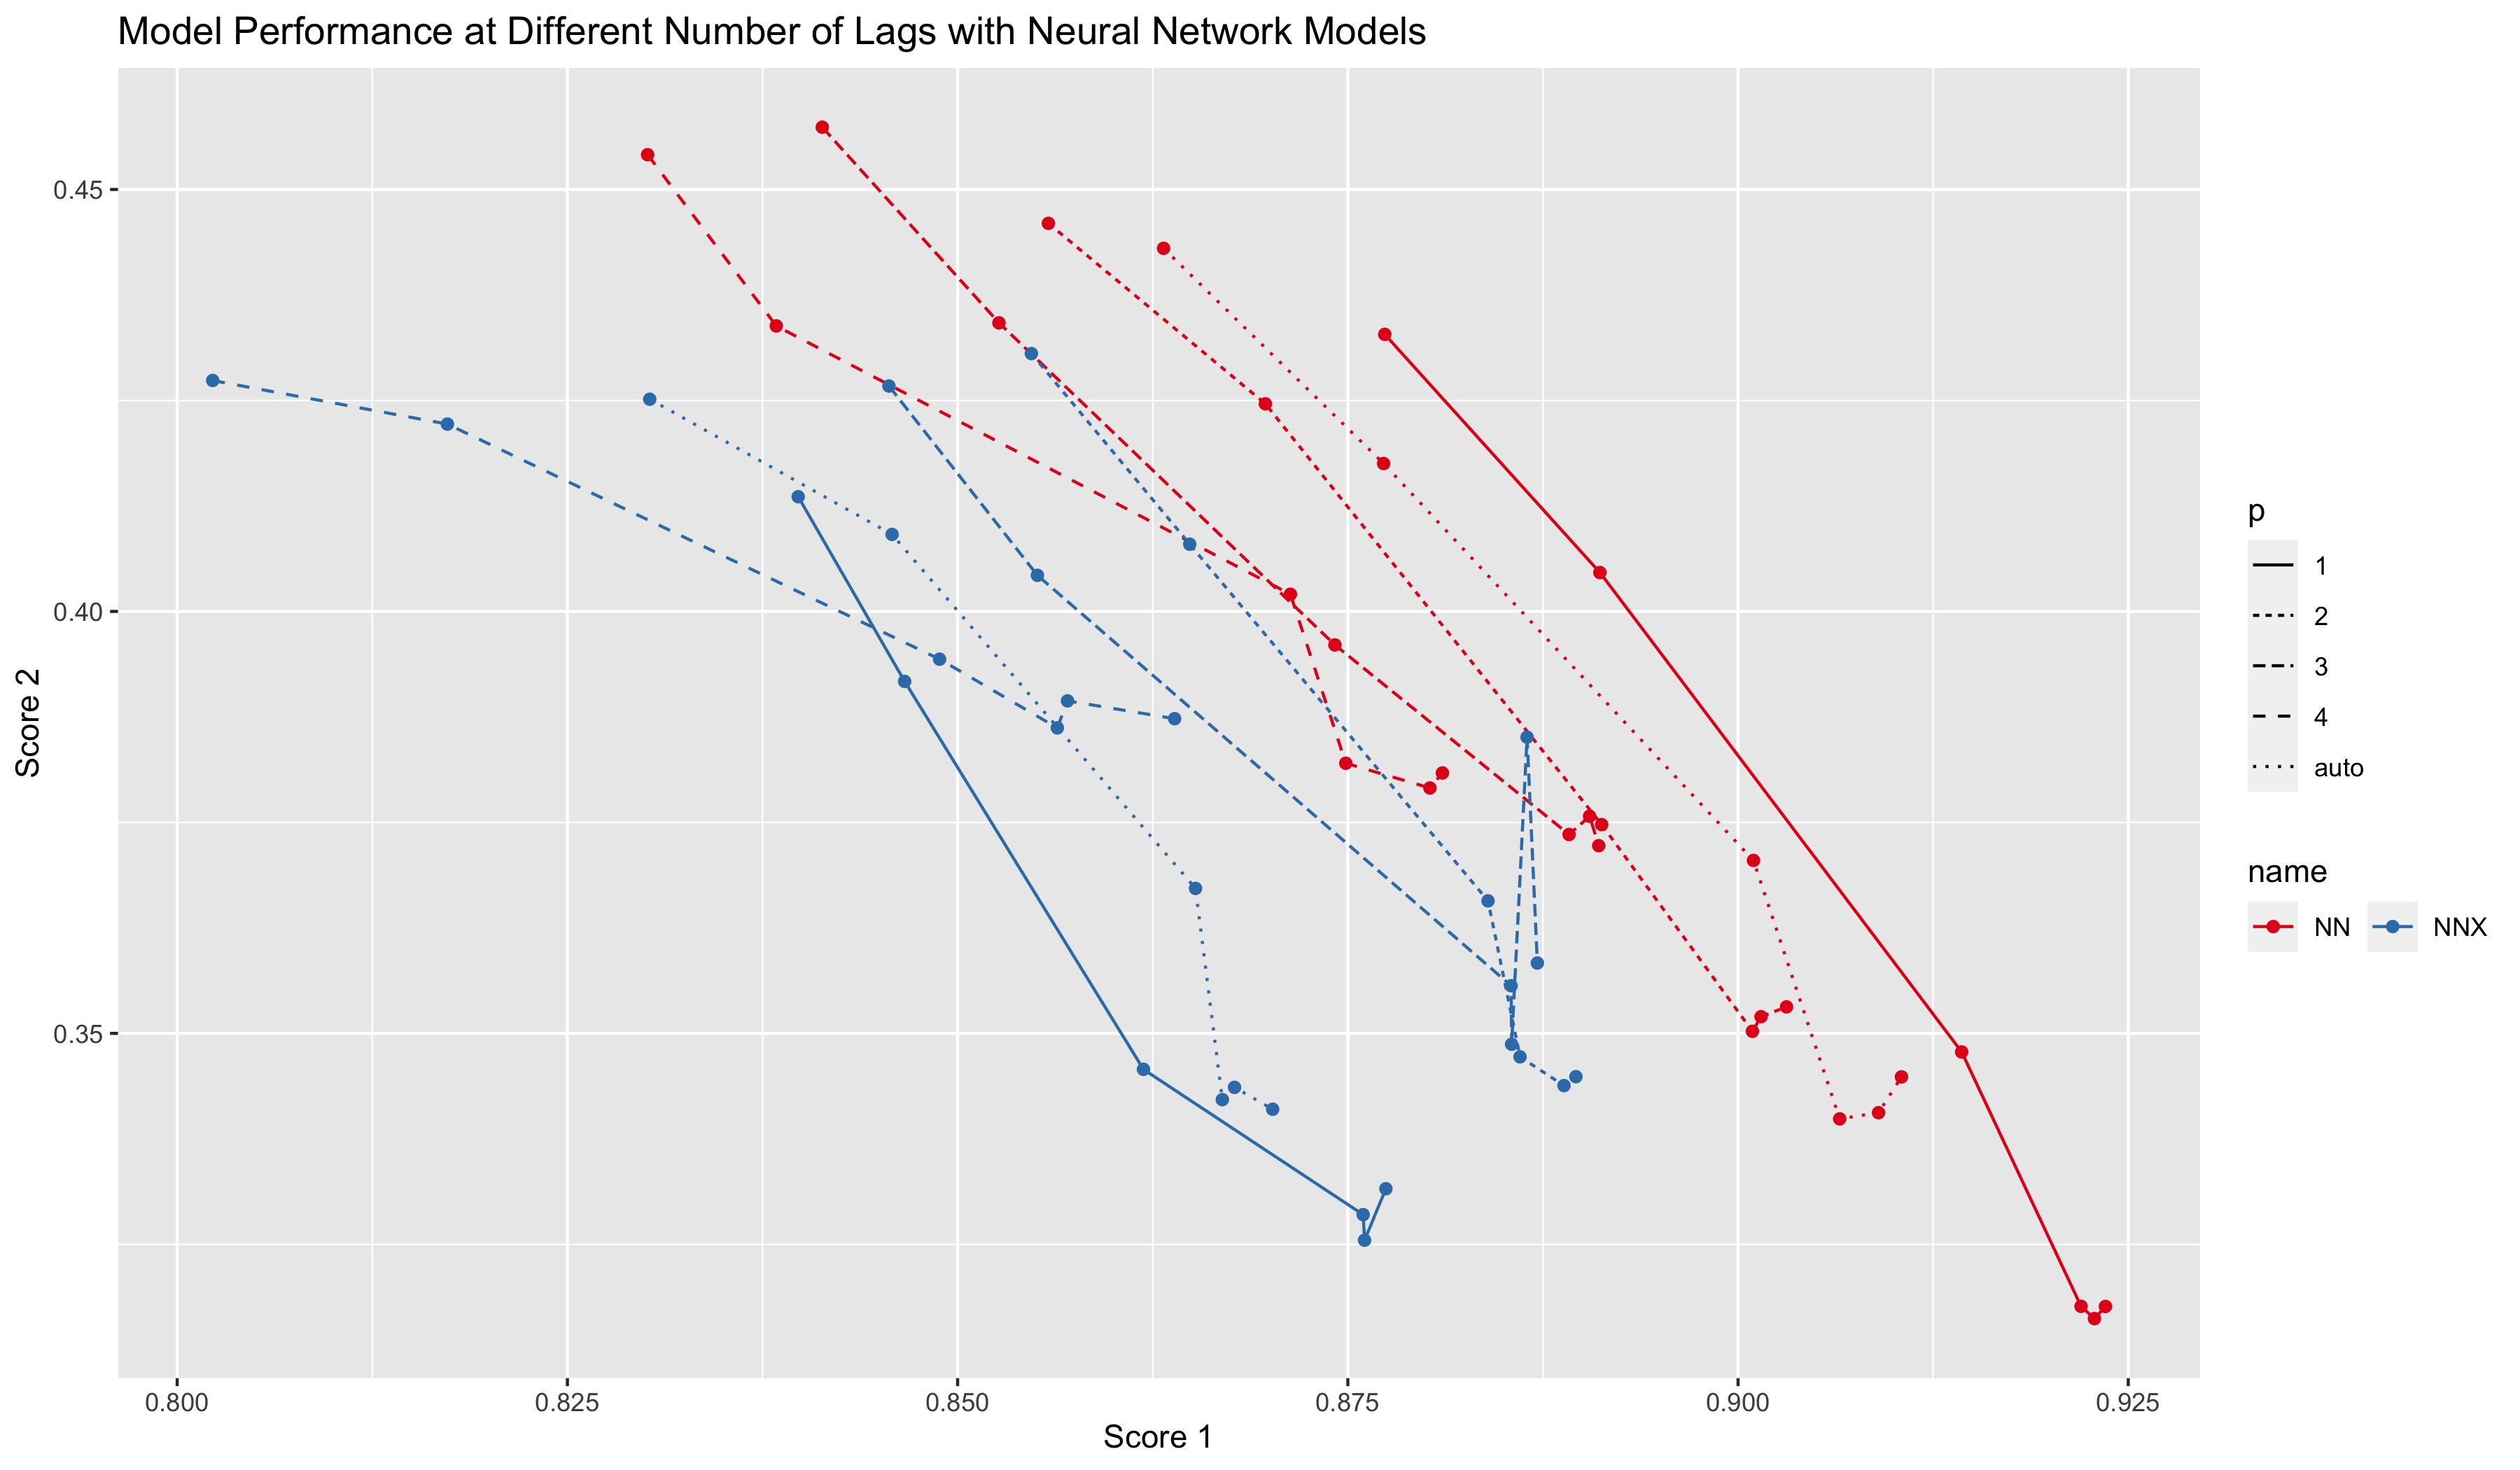
\includegraphics[width = 0.8\textwidth]{images/ModelPerformanceatDifferentNumberofLagswithNeuralNetworkModels.png}
    \label{fig:fig1.3.7}
\end{figure}

\begin{longtable}[htbp]{l|l|l|*{4}{c}}
  \caption{Configuration and Result of NN Model with Different lags}
  \label{tab:tab1.3.7} \\
  \textbf{model name} & \textbf{p} & \textbf{cut off prob} & \textbf{score 1} &
  \textbf{score 1 weight} & \textbf{score 2} & \textbf{score 2 weight} \\
      \hline
      NN & 1 & 0.001 & 0.9228 & 46859 & 0.3162 & 59249\\
      NN & 1 & 0.003 & 0.9235 & 46794 & 0.3176 & 59249\\
      NN & 1 & 0.005 & 0.9220 & 46972 & 0.3177 & 59249\\
      NN & 1 & 0.010 & 0.9143 & 48416 & 0.3478 & 59249\\
      NN & 1 & 0.030 & 0.8911 & 50528 & 0.4046 & 59249\\
      NN & 1 & 0.050 & 0.8774 & 52016 & 0.4328 & 59249\\
      NN & 2 & 0.001 & 0.9009 & 47134 & 0.3502 & 59249\\
      NN & 2 & 0.003 & 0.9015 & 47459 & 0.3520 & 59249\\
      NN & 2 & 0.005 & 0.9031 & 47391 & 0.3531 & 59249\\
      NN & 2 & 0.010 & 0.8913 & 48640 & 0.3747 & 59249\\
      NN & 2 & 0.030 & 0.8697 & 50890 & 0.4246 & 59249\\
      NN & 2 & 0.050 & 0.8558 & 52225 & 0.4460 & 59249\\
      NN & 3 & 0.001 & 0.8905 & 49009 & 0.3757 & 59249\\
      NN & 3 & 0.003 & 0.8892 & 48680 & 0.3736 & 59249\\
      NN & 3 & 0.005 & 0.8911 & 48482 & 0.3722 & 59249\\
      NN & 3 & 0.010 & 0.8742 & 49901 & 0.3960 & 59249\\
      NN & 3 & 0.030 & 0.8526 & 52100 & 0.4342 & 59249\\
      NN & 3 & 0.050 & 0.8413 & 53147 & 0.4574 & 59249\\
      NN & 4 & 0.001 & 0.8811 & 48268 & 0.3809 & 59249\\
      NN & 4 & 0.003 & 0.8749 & 48861 & 0.3820 & 59249\\
      NN & 4 & 0.005 & 0.8803 & 48171 & 0.3791 & 59249\\
      NN & 4 & 0.010 & 0.8713 & 50536 & 0.4020 & 59249\\
      NN & 4 & 0.030 & 0.8384 & 52674 & 0.4338 & 59249\\
      NN & 4 & 0.050 & 0.8301 & 53968 & 0.4541 & 59249\\
      NN & auto & 0.001 & 0.9090 & 47824 & 0.3406 & 59249\\
      NN & auto & 0.003 & 0.9065 & 47792 & 0.3399 & 59249\\
      NN & auto & 0.005 & 0.9105 & 47883 & 0.3448 & 59249\\
      NN & auto & 0.010 & 0.9010 & 49105 & 0.3705 & 59249\\
      NN & auto & 0.030 & 0.8773 & 51293 & 0.4175 & 59249\\
      NN & auto & 0.050 & 0.8632 & 52966 & 0.4430 & 59249\\
      NNX & 1 & 0.001 & 0.8761 & 46059 & 0.3255 & 59249\\
      NNX & 1 & 0.003 & 0.8760 & 46211 & 0.3285 & 59249\\
      NNX & 1 & 0.005 & 0.8774 & 46360 & 0.3316 & 59249\\
      NNX & 1 & 0.001 & 0.8619 & 47880 & 0.3457 & 59249\\
      NNX & 1 & 0.030 & 0.8466 & 49617 & 0.3917 & 59249\\
      NNX & 1 & 0.050 & 0.8398 & 50895 & 0.4136 & 59249\\
      NNX & 2 & 0.001 & 0.8888 & 45568 & 0.3438 & 59249\\
      NNX & 2 & 0.003 & 0.8896 & 45476 & 0.3449 & 59249\\
      NNX & 2 & 0.005 & 0.8860 & 46557 & 0.3472 & 59249\\
      NNX & 2 & 0.010 & 0.8840 & 47449 & 0.3657 & 59249\\
      NNX & 2 & 0.030 & 0.8649 & 50322 & 0.4080 & 59249\\
      NNX & 2 & 0.050 & 0.8547 & 52460 & 0.4306 & 59249\\
      NNX & 3 & 0.001 & 0.8855 & 45692 & 0.3487 & 59249\\
      NNX & 3 & 0.005 & 0.8871 & 46554 & 0.3583 & 59249\\
      NNX & 3 & 0.010 & 0.8865 & 48592 & 0.3851 & 59249\\
      NNX & 3 & 0.030 & 0.8551 & 50239 & 0.4043 & 59249\\
      NNX & 3 & 0.050 & 0.8456 & 51600 & 0.4267 & 59249\\
      NNX & 4 & 0.001 & 0.8564 & 48596 & 0.3862 & 59249\\
      NNX & 4 & 0.003 & 0.8639 & 48671 & 0.3873 & 59249\\
      NNX & 4 & 0.005 & 0.8570 & 49700 & 0.3894 & 59249\\
      NNX & 4 & 0.010 & 0.8488 & 49995 & 0.3943 & 59249\\
      NNX & 4 & 0.030 & 0.8173 & 51421 & 0.4222 & 59249\\
      NNX & 4 & 0.050 & 0.8023 & 52340 & 0.4274 & 59249\\
      NNX & auto & 0.001 & 0.8702 & 47413 & 0.3410 & 59249\\
      NNX & auto & 0.003 & 0.8677 & 47460 & 0.3436 & 59249\\
      NNX & auto & 0.005 & 0.8670 & 46978 & 0.3421 & 59249\\
      NNX & auto & 0.010 & 0.8652 & 48739 & 0.3672 & 59249\\
      NNX & auto & 0.030 & 0.8458 & 51894 & 0.4091 & 59249\\
      NNX & auto & 0.050 & 0.8303 & 52173 & 0.4251 & 59249\\
\end{longtable}

\subsubsection{Aggregation VS Extrapolation}
Ref to Section 1.4, include Fig \ref{fig:fig1.4.1} and Table \ref{tab:tab1.4.1}.

\begin{figure}[htbp]
    \caption{Trade-off Curves for Different Extrapolation Steps}
    \centering
    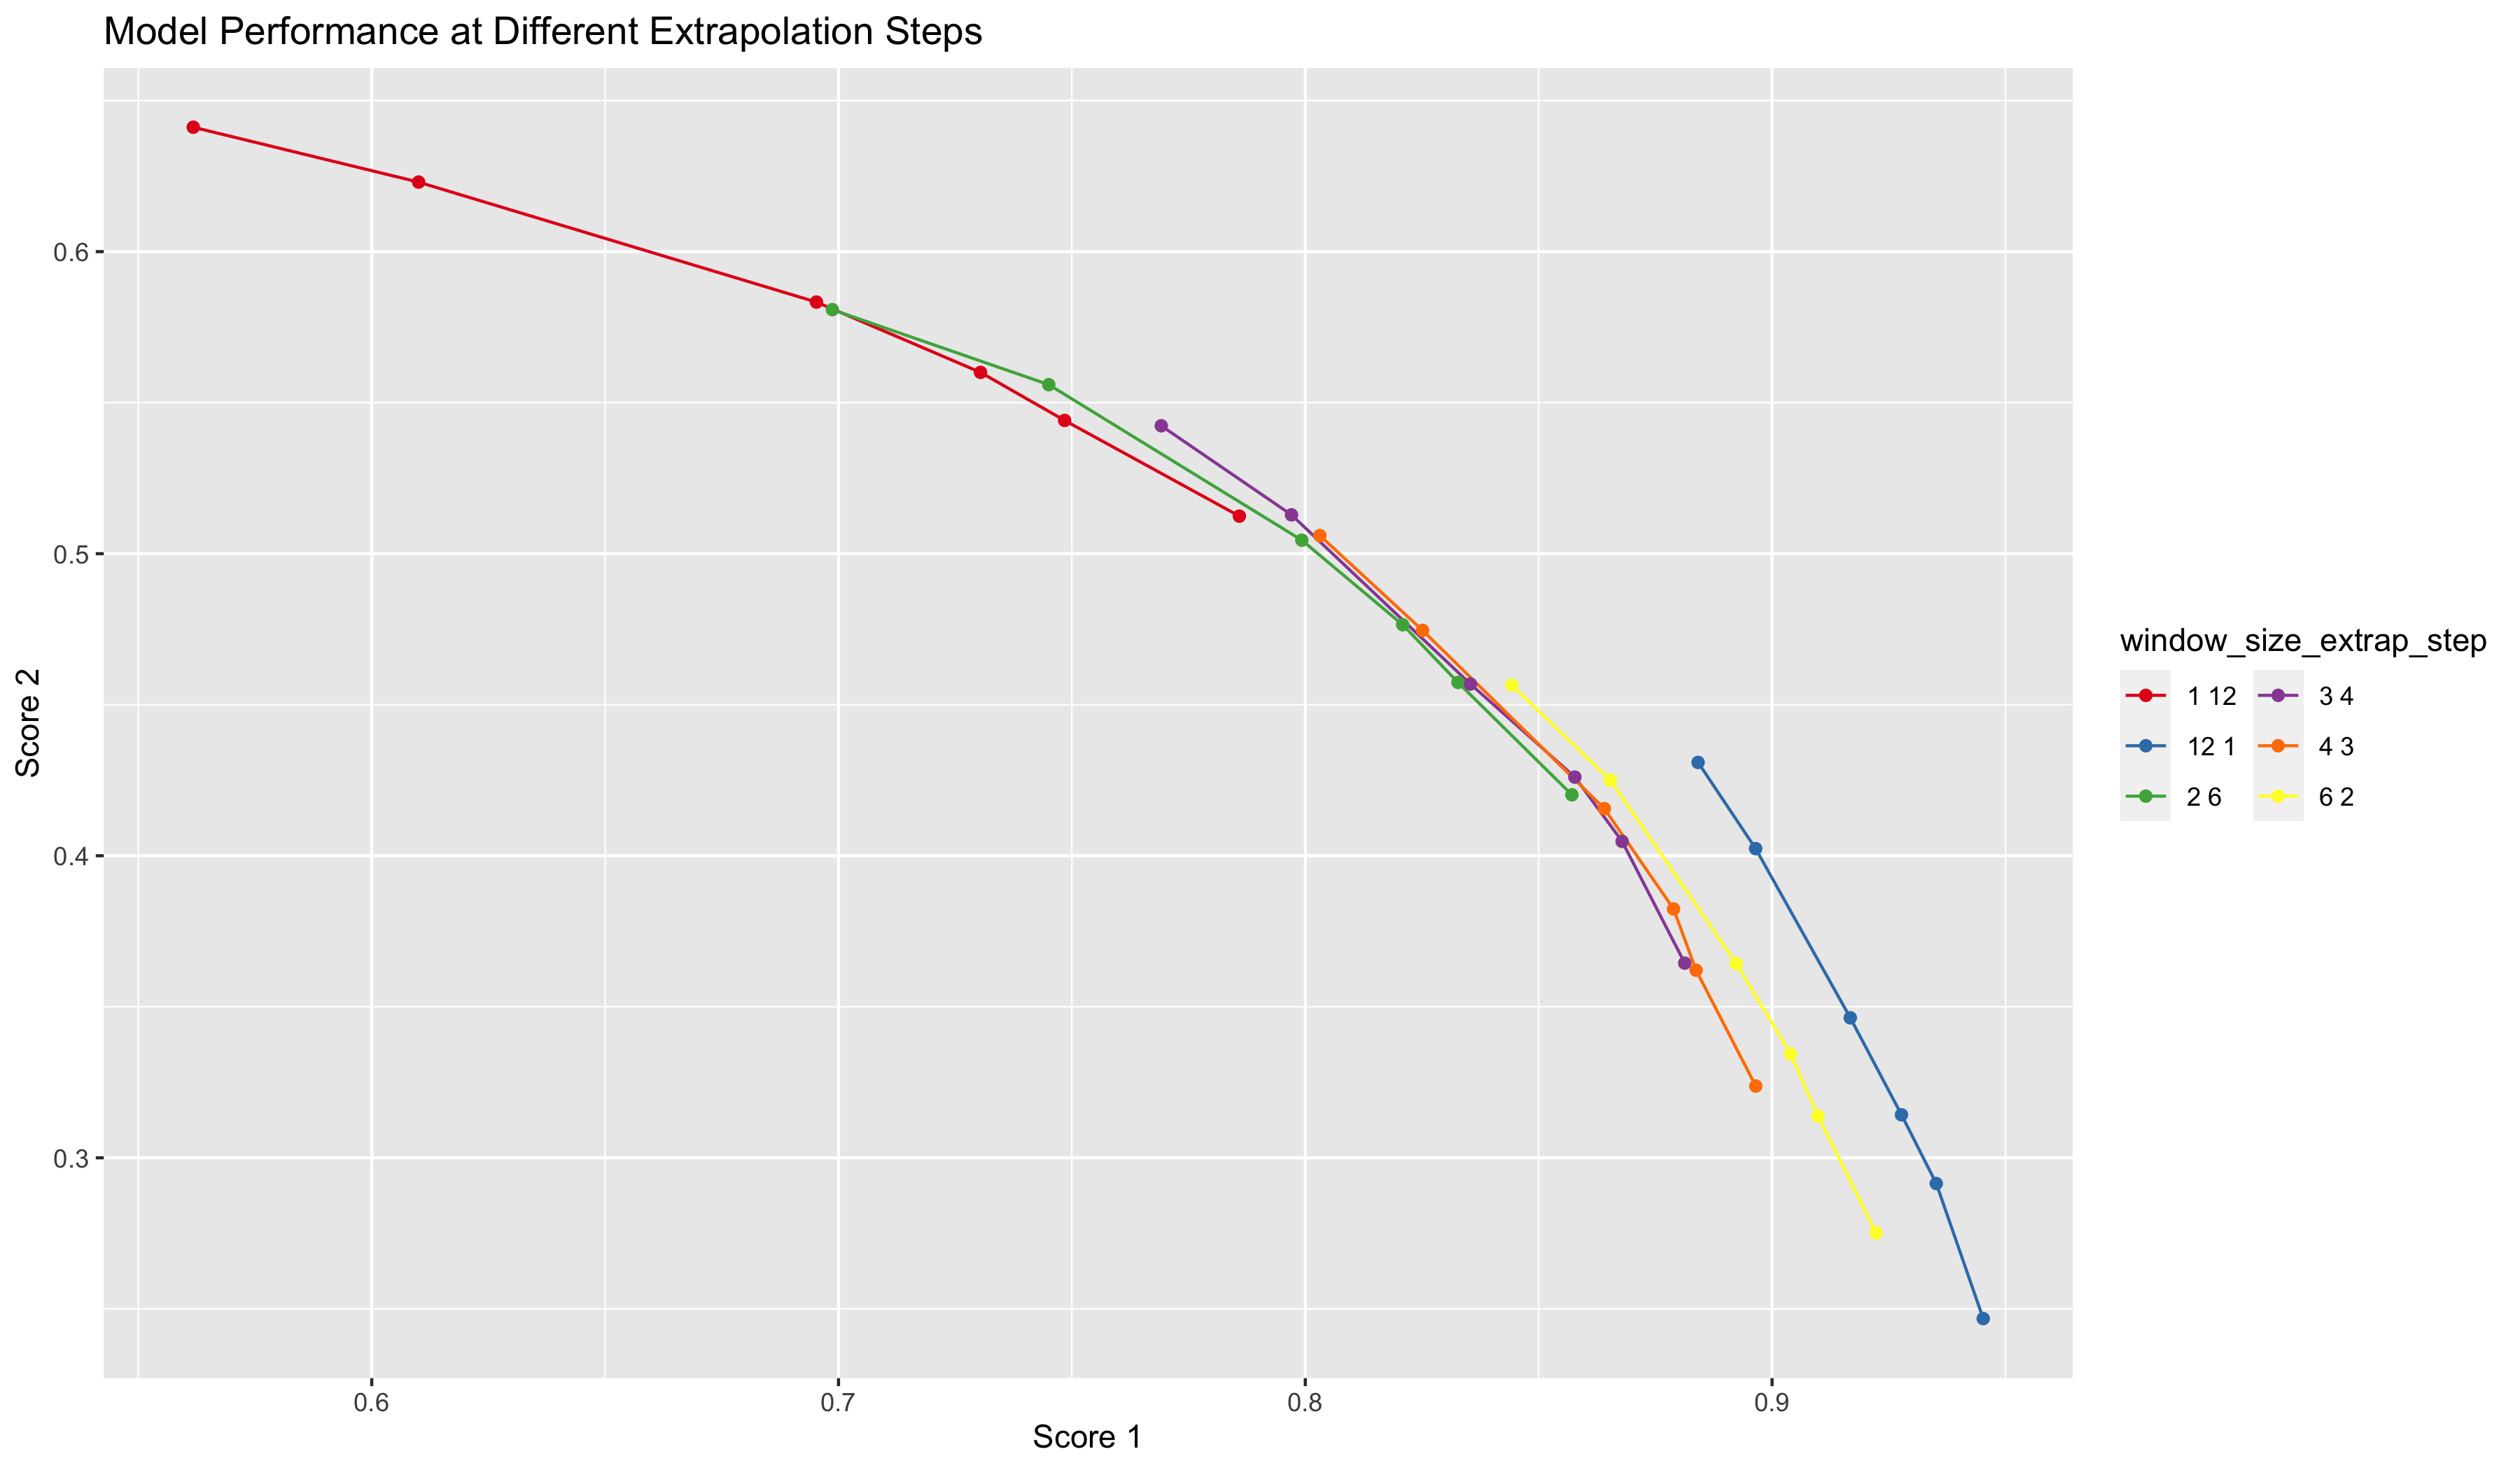
\includegraphics[width = 0.8\textwidth]{images/ModelPerformanceatDifferentExtrapolationSteps.png}
    \label{fig:fig1.4.1}
\end{figure}

\begin{longtable}[htbp]{l|l|l|*{4}{c}}
    \caption{Configuration and Result of AR1 Model with Different Extrapolation Steps}
    \label{tab:tab1.4.1} \\
    \textbf{window size} & \textbf{extrap step} & \textbf{cut off prob} &
    \textbf{score 1} & \textbf{score 1 weight} & \textbf{score 2} &
    \textbf{score 2 weight} \\
    \hline
    12 & 1 & 0.001 & 0.9452 & 42981 & 0.2468 & 59249\\
    12 & 1 & 0.003 & 0.9352 & 46484 & 0.2915 & 59249\\
    12 & 1 & 0.005 & 0.9277 & 47487 & 0.3142 & 59249\\
    12 & 1 & 0.010 & 0.9168 & 48124 & 0.3463 & 59249\\
    12 & 1 & 0.030 & 0.8965 & 50300 & 0.4024 & 59249\\
    12 & 1 & 0.050 & 0.8841 & 52904 & 0.4309 & 59249\\
    6 & 2 & 0.001 & 0.9223 & 42894 & 0.2751 & 59249\\
    6 & 2 & 0.003 & 0.9099 & 44826 & 0.3138 & 59249\\
    6 & 2 & 0.005 & 0.9040 & 46383 & 0.3344 & 59249\\
    6 & 2 & 0.010 & 0.8923 & 47700 & 0.3642 & 59249\\
    6 & 2 & 0.030 & 0.8654 & 52518 & 0.4250 & 59249\\
    6 & 2 & 0.050 & 0.8442 & 53601 & 0.4565 & 59249\\
    4 & 3 & 0.001 & 0.8965 & 44584 & 0.3237 & 59249\\
    4 & 3 & 0.003 & 0.8837 & 46569 & 0.3621 & 59249\\
    4 & 3 & 0.005 & 0.8789 & 49140 & 0.3824 & 59249\\
    4 & 3 & 0.010 & 0.8641 & 51370 & 0.4156 & 59249\\
    4 & 3 & 0.030 & 0.8251 & 53782 & 0.4746 & 59249\\
    4 & 3 & 0.050 & 0.8031 & 55304 & 0.5060 & 59249\\
    3 & 4 & 0.001 & 0.8813 & 46600 & 0.3645 & 59249\\
    3 & 4 & 0.003 & 0.8679 & 50354 & 0.4048 & 59249\\
    3 & 4 & 0.005 & 0.8577 & 52049 & 0.4260 & 59249\\
    3 & 4 & 0.010 & 0.8354 & 52424 & 0.4569 & 59249\\
    3 & 4 & 0.030 & 0.7970 & 54986 & 0.5129 & 59249\\
    3 & 4 & 0.050 & 0.7692 & 56591 & 0.5423 & 59249\\
    2 & 6 & 0.001 & 0.8571 & 50336 & 0.4202 & 59249\\
    2 & 6 & 0.003 & 0.8327 & 51827 & 0.4574 & 59249\\
    2 & 6 & 0.005 & 0.8209 & 52433 & 0.4765 & 59249\\
    2 & 6 & 0.010 & 0.7993 & 53626 & 0.5045 & 59249\\
    2 & 6 & 0.030 & 0.7450 & 56532 & 0.5560 & 59249\\
    2 & 6 & 0.050 & 0.6987 & 57175 & 0.5808 & 59249\\
    1 & 12 & 0.001 & 0.7859 & 52731 & 0.5124 & 59249\\
    1 & 12 & 0.003 & 0.7484 & 53427 & 0.5441 & 59249\\
    1 & 12 & 0.005 & 0.7304 & 54588 & 0.5600 & 59249\\
    1 & 12 & 0.010 & 0.6953 & 56316 & 0.5833 & 59249\\
    1 & 12 & 0.030 & 0.6100 & 56991 & 0.6230 & 59249\\
    1 & 12 & 0.050 & 0.5618 & 57010 & 0.6412 & 59249\\
\end{longtable}

\subsubsection{Offline Training VS Online Training}
Ref to Section 1.5, include Fig \ref{fig:fig1.5.1}, Table \ref{tab:tab1.5.1},
Fig \ref{fig:fig1.5.2}, Table \ref{tab:tab1.5.2}, Fig \ref{fig:fig1.5.3}, and
Table \ref{tab:tab1.5.3}.

\begin{figure}
    \caption{Trade-off Curves for Different Training Policies}
    \centering
    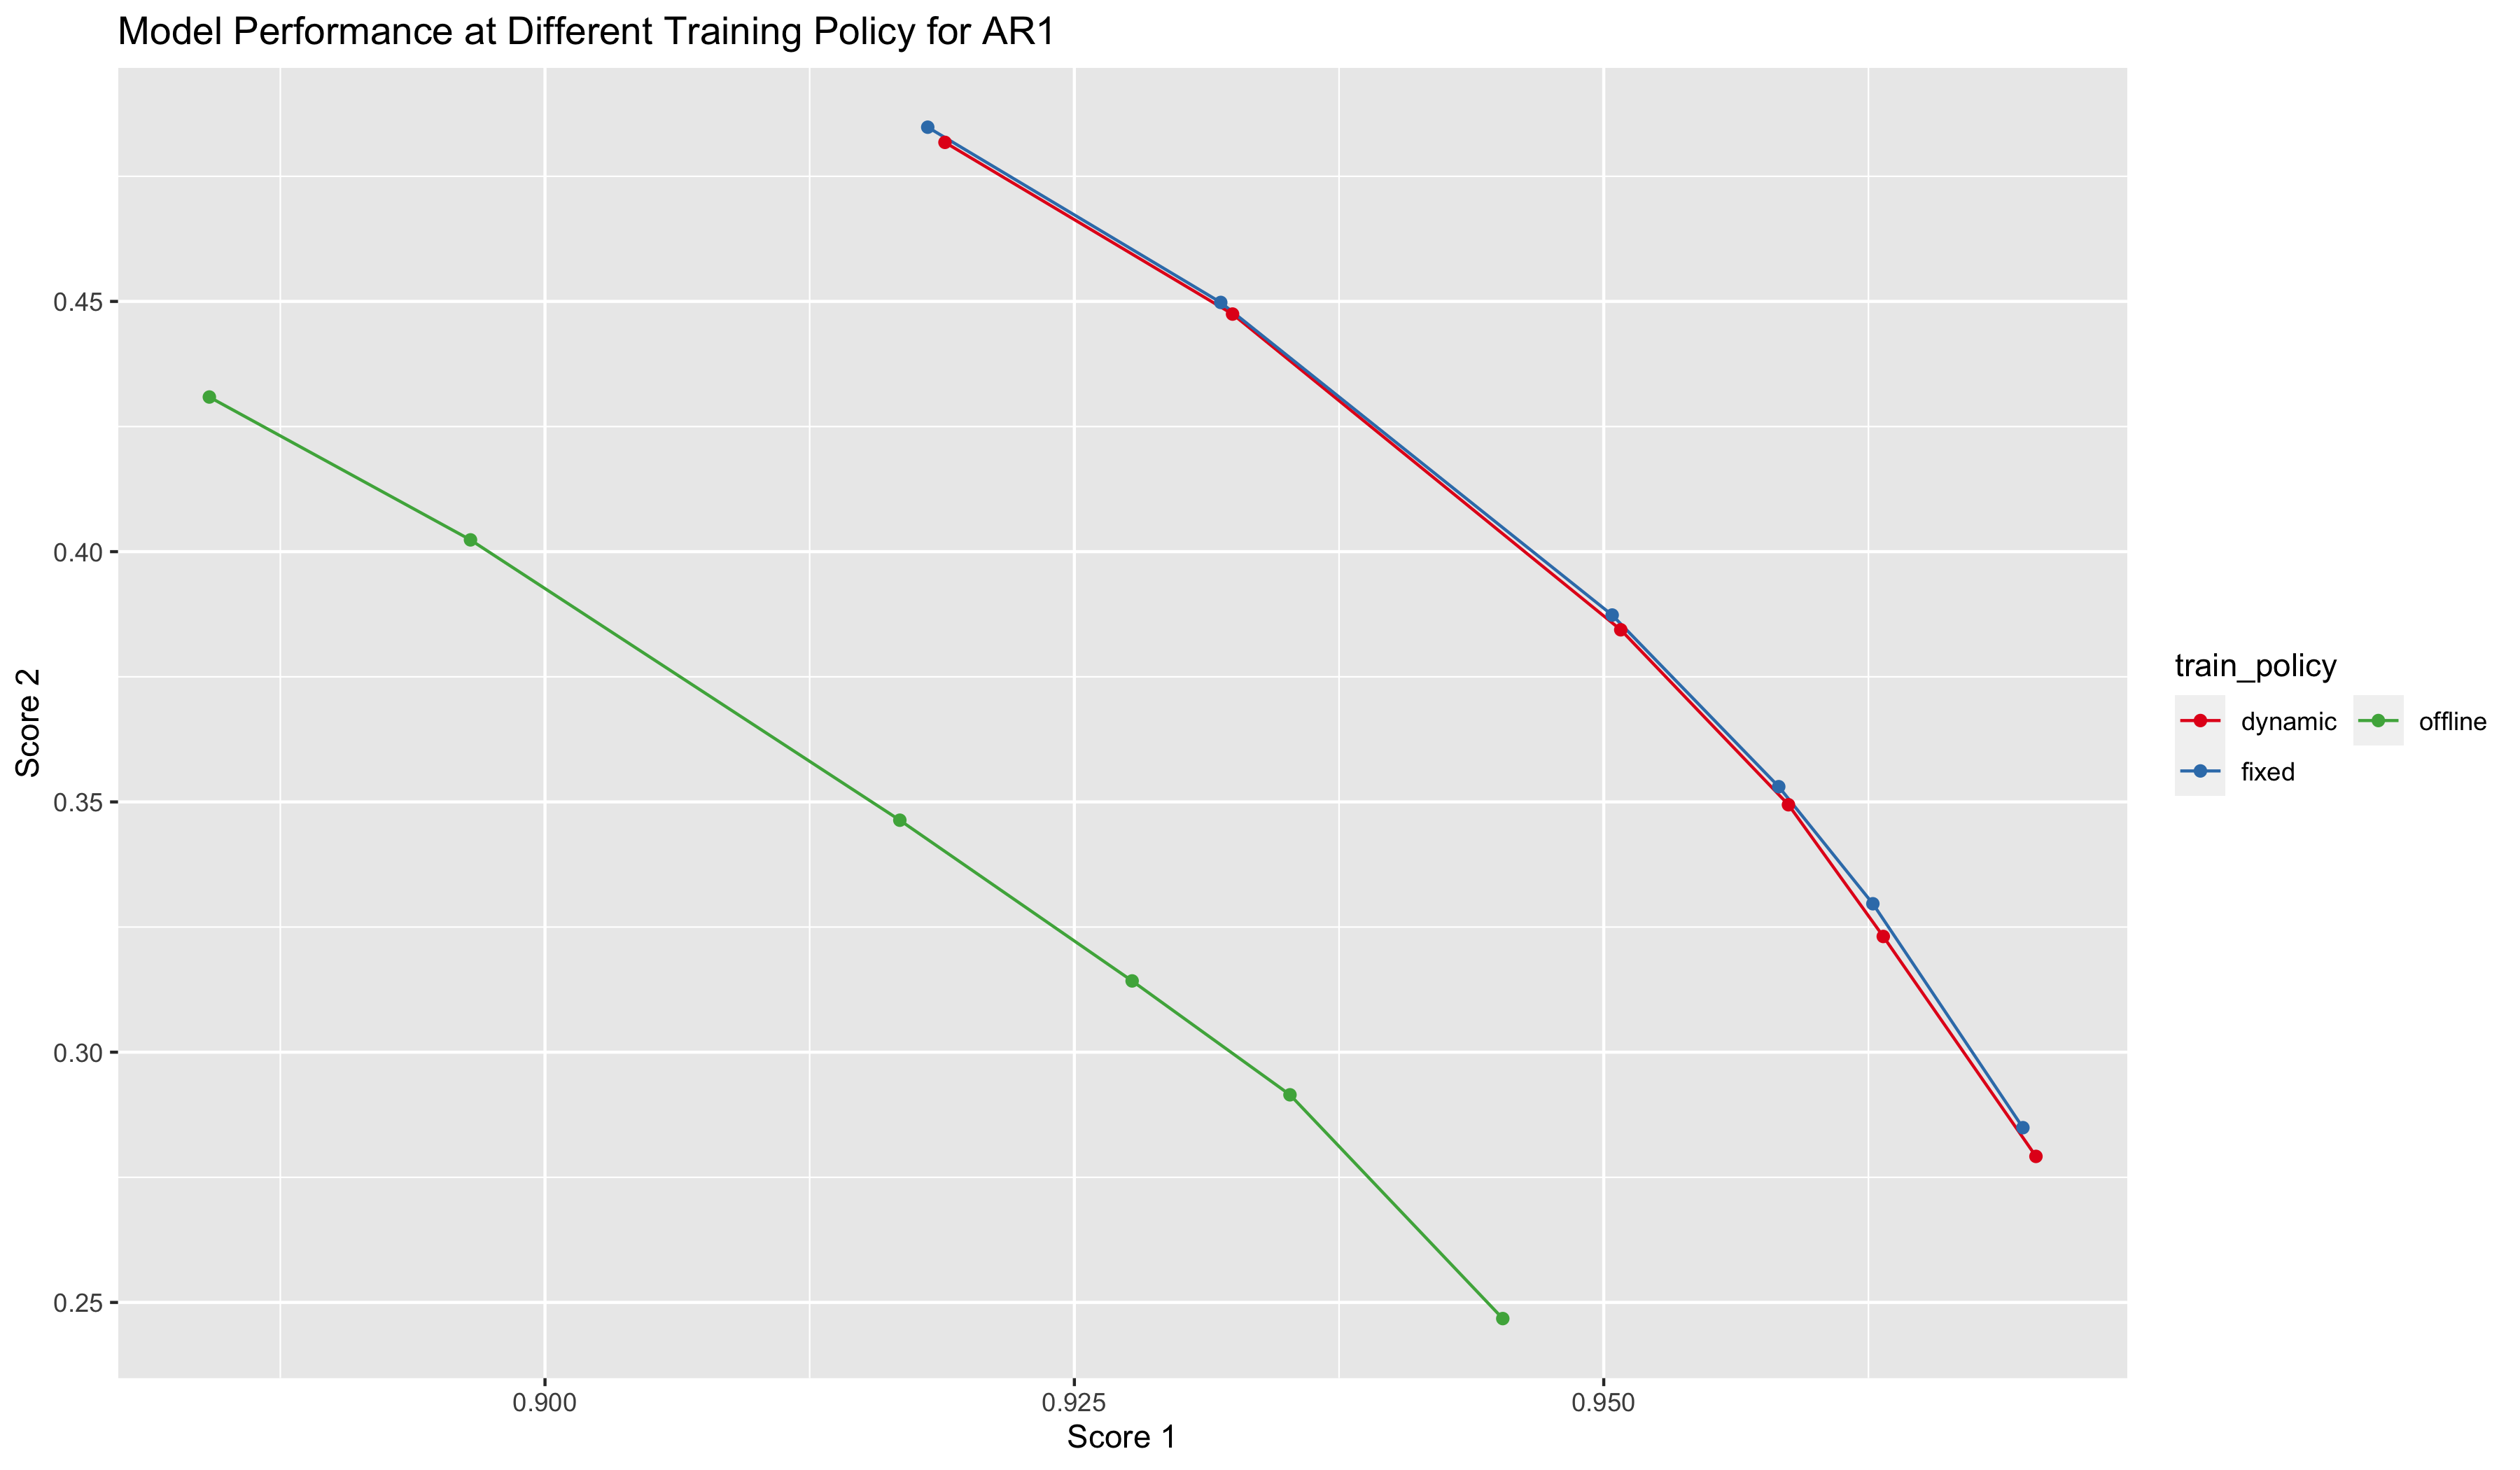
\includegraphics[width = 0.8\textwidth]{images/ModelPerformanceatDifferentTrainingPolicyforAR1.png}
    \label{fig:fig1.5.1}
\end{figure}

\begin{table}[htbp]
  \begin{center}
    \caption{Configuration and Result of AR1 Model with Different Training Policies}
    \label{tab:tab1.5.1}
    \begin{tabular}{l|l|*{4}{c}} \textbf{training policy} & \textbf{cut off
      prob} & \textbf{score 1} & \textbf{score 1 weight} & \textbf{score 2} &
      \textbf{score 2 weight} \\
      \hline
      offline & 0.001 & 0.9452 & 42981 & 0.2468 & 59249\\
      offline & 0.003 & 0.9352 & 46484 & 0.2915 & 59249\\
      offline & 0.005 & 0.9277 & 47487 & 0.3142 & 59249\\
      offline & 0.010 & 0.9168 & 48124 & 0.3463 & 59249\\
      offline & 0.030 & 0.8965 & 50300 & 0.4024 & 59249\\
      offline & 0.050 & 0.8841 & 52904 & 0.4309 & 59249\\
      fixed & 0.001 & 0.9698 & 42245 & 0.2849 & 59249\\
      fixed & 0.003 & 0.9627 & 45239 & 0.3297 & 59249\\
      fixed & 0.005 & 0.9583 & 46435 & 0.3530 & 59249\\
      fixed & 0.010 & 0.9504 & 47518 & 0.3873 & 59249\\
      fixed & 0.030 & 0.9319 & 50406 & 0.4498 & 59249\\
      fixed & 0.050 & 0.9181 & 52841 & 0.4848 & 59249\\
      dynamic & 0.001 & 0.9704 & 42449 & 0.2792 & 59249\\
      dynamic & 0.003 & 0.9632 & 45137 & 0.3231 & 59249\\
      dynamic & 0.005 & 0.9587 & 46419 & 0.3494 & 59249\\
      dynamic & 0.010 & 0.9508 & 47422 & 0.3844 & 59249\\
      dynamic & 0.030 & 0.9325 & 50363 & 0.4475 & 59249\\
      dynamic & 0.050 & 0.9189 & 52866 & 0.4818 & 59249\\
    \end{tabular}
  \end{center}
\end{table}

\begin{figure}
    \caption{Model Performance for Different Batch Size of Dynamic Training}
    \centering
    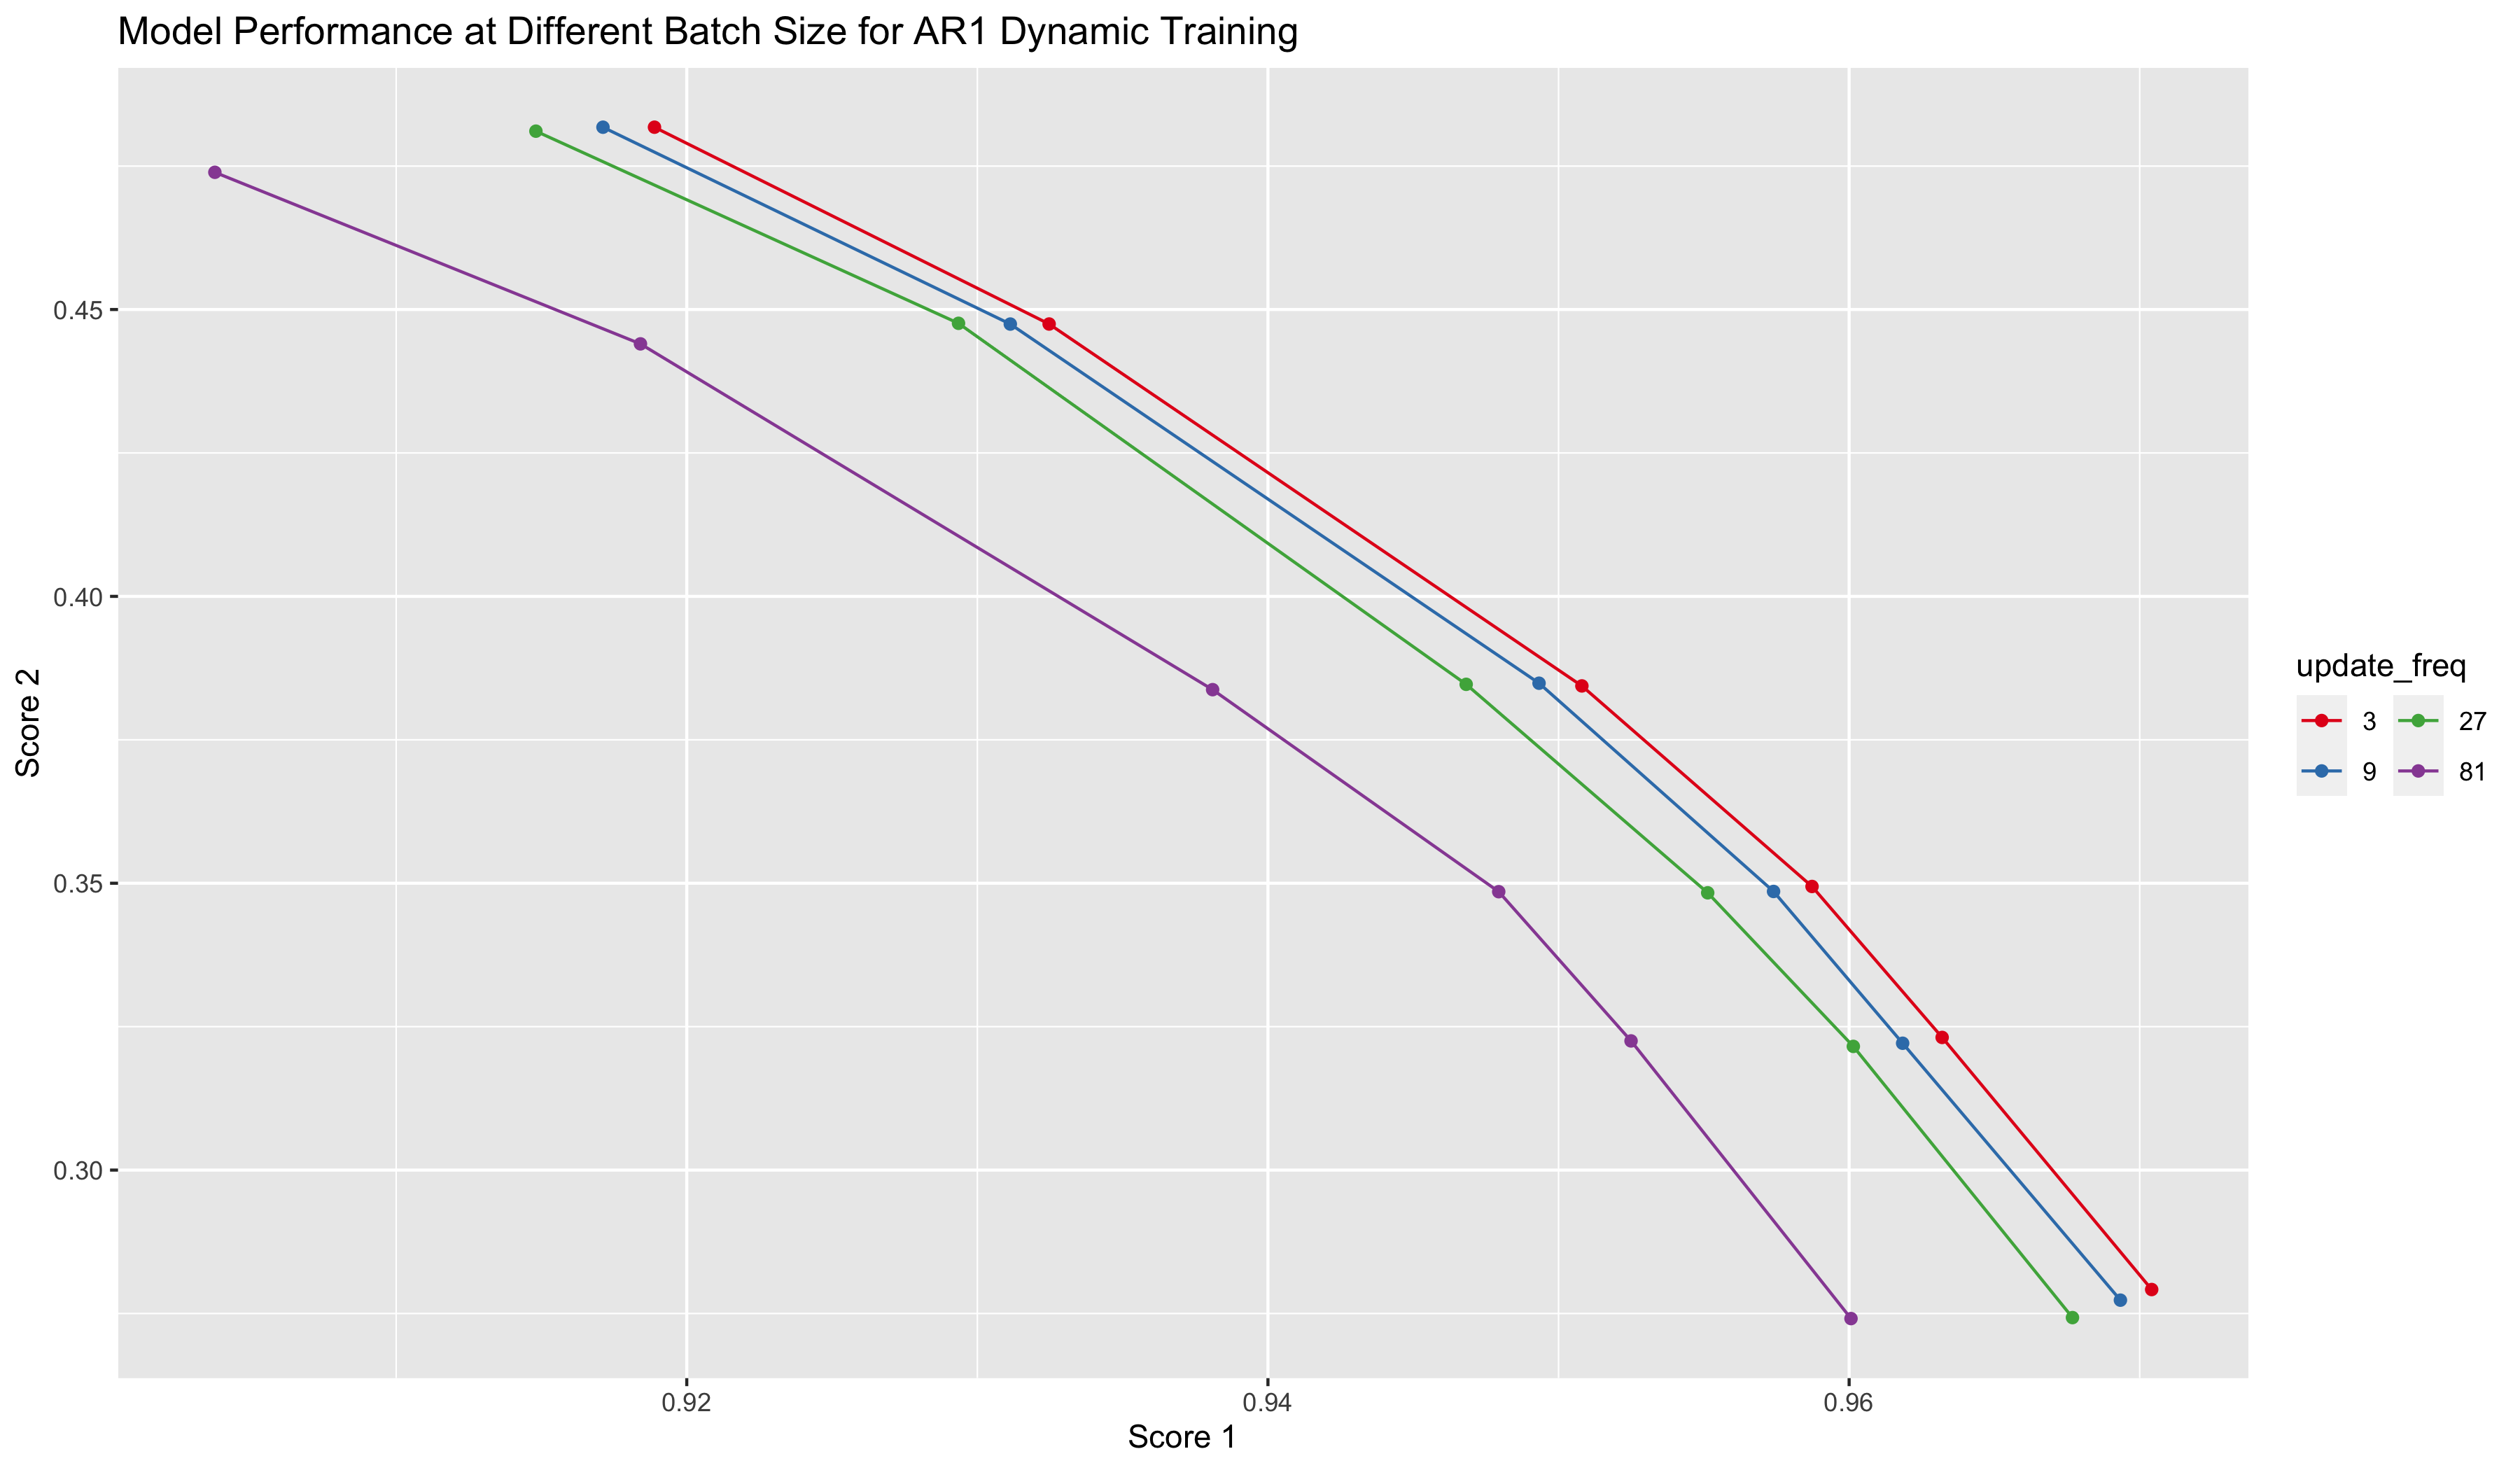
\includegraphics[width = 0.8\textwidth]{images/ModelPerformanceatDifferentBatchSizeforAR1DynamicTraining.png}
    \label{fig:fig1.5.2}
\end{figure}

\begin{table}[htbp]
  \begin{center}
    \caption{Configuration and Result of AR1 Model with Different Batch Size of Dynamic Training}
    \label{tab:tab1.5.2}
    \begin{tabular}{l|l|*{4}{c}} \textbf{batch size} & \textbf{cut off prob} &
      \textbf{score 1} & \textbf{score 1 weight} & \textbf{score 2} &
      \textbf{score 2 weight} \\
      \hline
      3 & 0.001 & 0.9704 & 42449 & 0.2792 & 59249\\
      3 & 0.003 & 0.9632 & 45137 & 0.3231 & 59249\\
      3 & 0.005 & 0.9587 & 46419 & 0.3494 & 59249\\
      3 & 0.010 & 0.9508 & 47422 & 0.3844 & 59249\\
      3 & 0.030 & 0.9325 & 50363 & 0.4475 & 59249\\
      3 & 0.050 & 0.9189 & 52866 & 0.4818 & 59249\\
      9 & 0.001 & 0.9693 & 42427 & 0.2773 & 59249\\
      9 & 0.003 & 0.9618 & 45075 & 0.3221 & 59249\\
      9 & 0.005 & 0.9574 & 46478 & 0.3486 & 59249\\
      9 & 0.010 & 0.9493 & 47562 & 0.3849 & 59249\\
      9 & 0.030 & 0.9311 & 50533 & 0.4475 & 59249\\
      9 & 0.050 & 0.9171 & 52966 & 0.4818 & 59249\\
      27 & 0.001 & 0.9677 & 42087 & 0.2743 & 59249\\
      27 & 0.003 & 0.9601 & 45188 & 0.3216 & 59249\\
      27 & 0.005 & 0.9551 & 46716 & 0.3483 & 59249\\
      27 & 0.010 & 0.9468 & 47764 & 0.3847 & 59249\\
      27 & 0.030 & 0.9294 & 50702 & 0.4476 & 59249\\
      27 & 0.050 & 0.9148 & 53010 & 0.4811 & 5924\\
      81 & 0.001 & 0.9601 & 40290 & 0.2741 & 56561\\
      81 & 0.003 & 0.9525 & 43764 & 0.3225 & 56561\\
      81 & 0.005 & 0.9479 & 45007 & 0.3485 & 56561\\
      81 & 0.010 & 0.9381 & 45813 & 0.3837 & 56561\\
      81 & 0.030 & 0.9184 & 48803 & 0.4440 & 56561\\
      81 & 0.050 & 0.9038 & 50572 & 0.4739 & 56561\\
    \end{tabular}
  \end{center}
\end{table}

\begin{figure}
    \caption{Different Models with Different Training Policy}
    \centering
    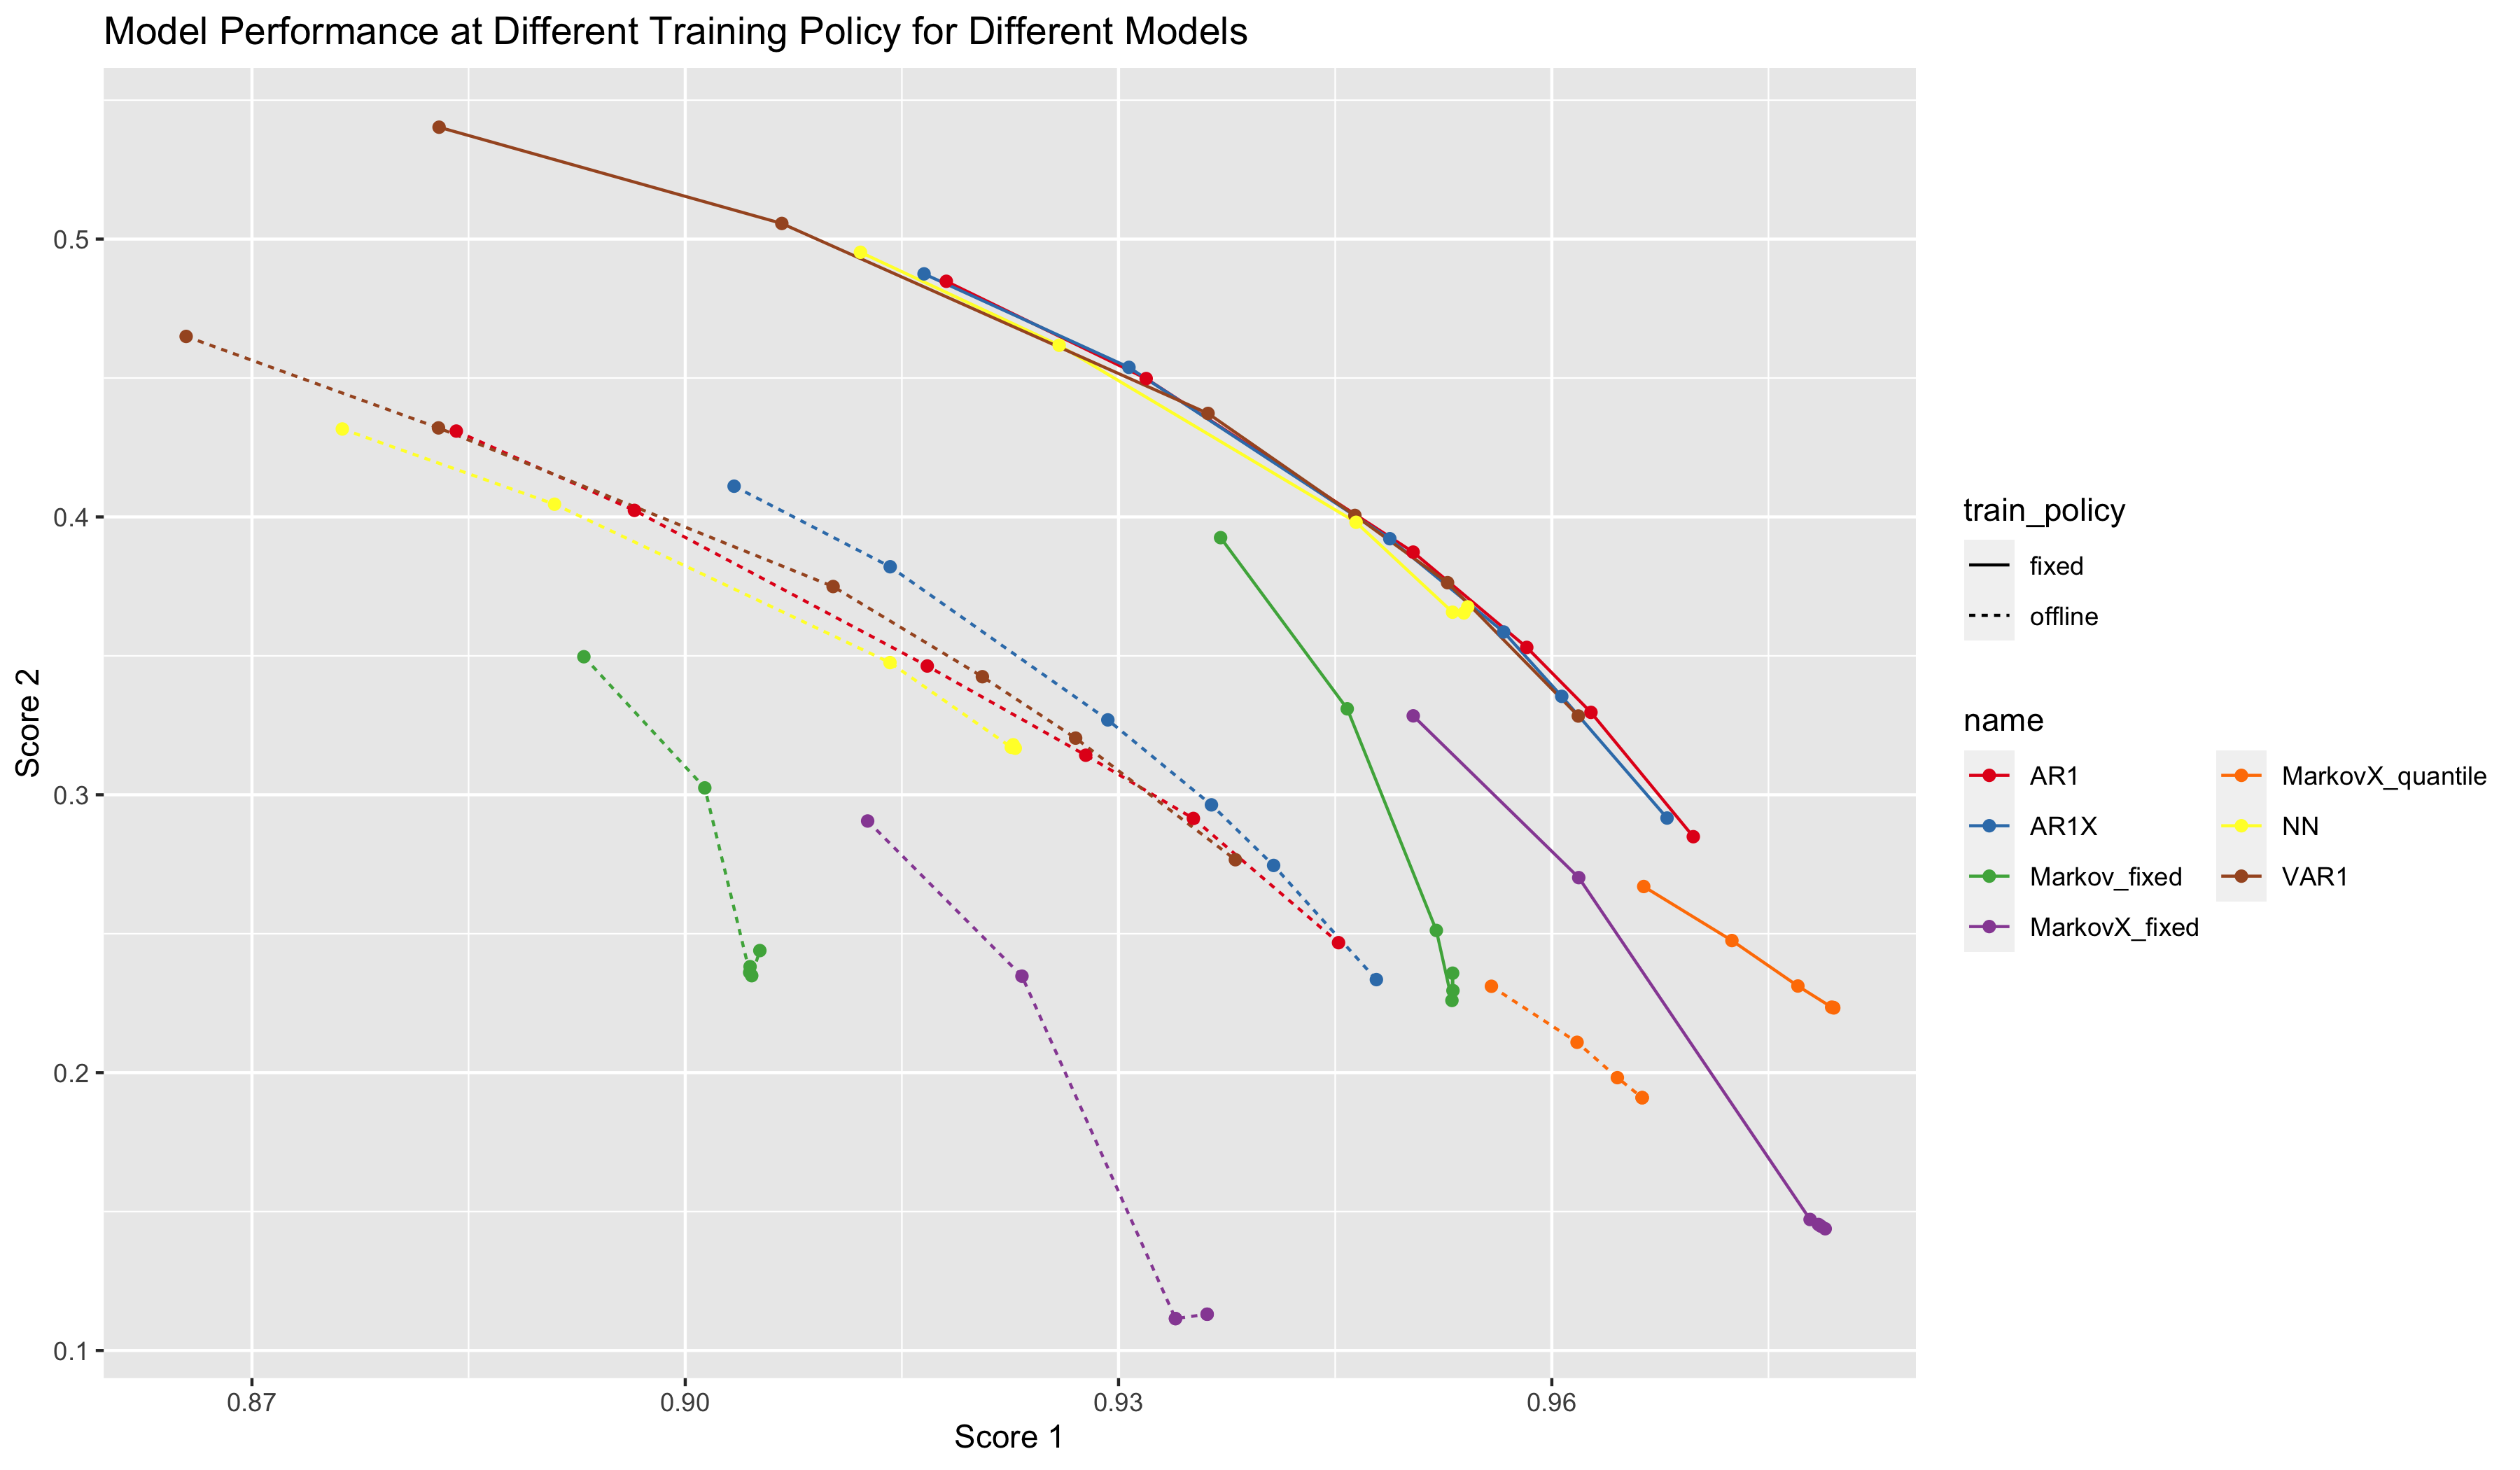
\includegraphics[width = 0.8\textwidth]{images/ModelPerformanceatDifferentModelswithDifferentTrainingPolicy.png}
    \label{fig:fig1.5.3}
\end{figure}

\begin{longtable}[htbp]{l|l|l|*{4}{c}}
    \caption{Configuration and Result of Different Models and Different Training Policy}
    \label{tab:tab1.5.3} \\
    \textbf{model} & \textbf{training policy} & \textbf{cut off prob} &
    \textbf{score 1} & \textbf{score 1 weight} & \textbf{score 2} &
    \textbf{score 2 weight} \\
    \hline
    AR1 & fixed & 0.001 & 0.9698 & 42245 & 0.2849 & 59249\\
    AR1 & fixed & 0.003 & 0.9627 & 45239 & 0.3297 & 59249\\
    AR1 & fixed & 0.005 & 0.9583 & 46435 & 0.3530 & 59249\\
    AR1 & fixed & 0.010 & 0.9504 & 47518 & 0.3873 & 59249\\
    AR1 & fixed & 0.030 & 0.9319 & 50406 & 0.4498 & 59249\\
    AR1 & fixed & 0.050 & 0.9181 & 52841 & 0.4848 & 59249\\
    AR1 & offline & 0.001 & 0.9452 & 42981 & 0.2468 & 59249\\
    AR1 & offline & 0.003 & 0.9352 & 46484 & 0.2915 & 59249\\
    AR1 & offline & 0.005 & 0.9277 & 47487 & 0.3142 & 59249\\
    AR1 & offline & 0.010 & 0.9168 & 48124 & 0.3463 & 59249\\
    AR1 & offline & 0.030 & 0.8965 & 50300 & 0.4024 & 59249\\
    AR1 & offline & 0.050 & 0.8841 & 52904 & 0.4309 & 59249\\
    AR1X & fixed & 0.001 & 0.9680 & 42594 & 0.2916 & 59249\\
    AR1X & fixed & 0.003 & 0.9607 & 45379 & 0.3354 & 59249\\
    AR1X & fixed & 0.005 & 0.9567 & 46476 & 0.3586 & 59249\\
    AR1X & fixed & 0.010 & 0.9488 & 47679 & 0.3922 & 59249\\
    AR1X & fixed & 0.030 & 0.9307 & 50578 & 0.4538 & 59249\\
    AR1X & fixed & 0.050 & 0.9165 & 52692 & 0.4875 & 59249\\
    AR1X & offline & 0.001 & 0.9479 & 41306 & 0.2335 & 59249\\
    AR1X & offline & 0.003 & 0.9407 & 43602 & 0.2746 & 59249\\
    AR1X & offline & 0.005 & 0.9364 & 44299 & 0.2964 & 59249\\
    AR1X & offline & 0.010 & 0.9293 & 45094 & 0.3270 & 59249\\
    AR1X & offline & 0.030 & 0.9142 & 47570 & 0.3821 & 59249\\
    AR1X & offline & 0.050 & 0.9034 & 50374 & 0.4111 & 59249\\
    Markov fixed & fixed & 0.001 & 0.9531 & 29904 & 0.2260 & 59249\\
    Markov fixed & fixed & 0.003 & 0.9532 & 30312 & 0.2295 & 59249\\
    Markov fixed & fixed & 0.005 & 0.9531 & 30917 & 0.2358 & 59249\\
    Markov fixed & fixed & 0.010 & 0.9520 & 32086 & 0.2512 & 59249\\
    Markov fixed & fixed & 0.030 & 0.9458 & 38918 & 0.3309 & 59249\\
    Markov fixed & fixed & 0.050 & 0.9371 & 42711 & 0.3925 & 59249\\
    Markov fixed & offline & 0.001 & 0.9046 & 29990 & 0.2349 & 59249\\
    Markov fixed & offline & 0.003 & 0.9045 & 30082 & 0.2360 & 59249\\
    Markov fixed & offline & 0.005 & 0.9045 & 30195 & 0.2381 & 59249\\
    Markov fixed & offline & 0.010 & 0.9052 & 31233 & 0.2439 & 59249\\
    Markov fixed & offline & 0.030 & 0.9014 & 37994 & 0.3025 & 59249\\
    Markov fixed & offline & 0.050 & 0.893 & 41058 & 0.3497 & 59249\\
    MarkovX fixed & fixed & 0.001 & 0.9789 & 21213 & 0.1438 & 59249\\
    MarkovX fixed & fixed & 0.003 & 0.9786 & 21296 & 0.1447 & 59249\\
    MarkovX fixed & fixed & 0.005 & 0.9785 & 21356 & 0.1454 & 59249\\
    MarkovX fixed & fixed & 0.010 & 0.9779 & 21520 & 0.1471 & 59249\\
    MarkovX fixed & fixed & 0.030 & 0.9619 & 34533 & 0.2702 & 59249\\
    MarkovX fixed & fixed & 0.050 & 0.9504 & 38975 & 0.3284 & 59249\\
    MarkovX fixed & offline & 0.001 & 0.9339 & 16849 & 0.1115 & 59249\\
    MarkovX fixed & offline & 0.003 & 0.9339 & 16849 & 0.1115 & 59249\\
    MarkovX fixed & offline & 0.005 & 0.9361 & 17443 & 0.1131 & 59249\\
    MarkovX fixed & offline & 0.010 & 0.9361 & 17443 & 0.1131 & 59249\\
    MarkovX fixed & offline & 0.030 & 0.9233 & 32287 & 0.2347 & 59249\\
    MarkovX fixed & offline & 0.050 & 0.9126 & 36591 & 0.2906 & 59249\\
    MarkovX quantile & fixed & 0.001 & 0.9795 & 55226 & 0.2233 & 59249\\
    MarkovX quantile & fixed & 0.003 & 0.9795 & 55241 & 0.2234 & 59249\\
    MarkovX quantile & fixed & 0.005 & 0.9794 & 55267 & 0.2236 & 59249\\
    MarkovX quantile & fixed & 0.010 & 0.9770 & 55437 & 0.2312 & 59249\\
    MarkovX quantile & fixed & 0.030 & 0.9725 & 55645 & 0.2475 & 59249\\
    MarkovX quantile & fixed & 0.050 & 0.9664 & 55860 & 0.2670 & 59249\\
    MarkovX quantile & offline & 0.001 & 0.9663 & 56511 & 0.1910 & 59249\\
    MarkovX quantile & offline & 0.003 & 0.9663 & 56511 & 0.1910 & 59249\\
    MarkovX quantile & offline & 0.005 & 0.9663 & 56511 & 0.1910 & 59249\\
    MarkovX quantile & offline & 0.010 & 0.9645 & 56650 & 0.1982 & 59249\\
    MarkovX quantile & offline & 0.030 & 0.9617 & 56650 & 0.2109 & 59249\\
    MarkovX quantile & offline & 0.050 & 0.9558 & 56650 & 0.2311 & 59249\\
    NN & fixed & 0.001 & 0.9531 & 46145 & 0.3657 & 59249\\
    NN & fixed & 0.003 & 0.9539 & 46128 & 0.3654 & 59249\\
    NN & fixed & 0.005 & 0.9542 & 46200 & 0.3676 & 59249\\
    NN & fixed & 0.010 & 0.9464 & 47654 & 0.3981 & 59249\\
    NN & fixed & 0.030 & 0.9259 & 50788 & 0.4618 & 59249\\
    NN & fixed & 0.050 & 0.9121 & 52772 & 0.4952 & 59249\\
    NN & offline & 0.001 & 0.9226 & 46819 & 0.3171 & 59249\\
    NN & offline & 0.003 & 0.9229 & 46805 & 0.3168 & 59249\\
    NN & offline & 0.005 & 0.9227 & 46923 & 0.3180 & 59249\\
    NN & offline & 0.010 & 0.9142 & 48401 & 0.3476 & 59249\\
    NN & offline & 0.030 & 0.8909 & 50527 & 0.4046 & 59249\\
    NN & offline & 0.050 & 0.8763 & 52059 & 0.4316 & 59249\\
    VAR1 & fixed & 0.001 & 0.9618 & 44987 & 0.3284 & 59249\\
    VAR1 & fixed & 0.003 & 0.9528 & 47098 & 0.3763 & 59249\\
    VAR1 & fixed & 0.005 & 0.9464 & 47952 & 0.4005 & 59249\\
    VAR1 & fixed & 0.010 & 0.9362 & 49559 & 0.4372 & 59249\\
    VAR1 & fixed & 0.030 & 0.9067 & 53679 & 0.5056 & 59249\\
    VAR1 & fixed & 0.050 & 0.8830 & 55244 & 0.5403 & 59249\\
    VAR1 & offline & 0.001 & 0.9381 & 44419 & 0.2766 & 59249\\
    VAR1 & offline & 0.003 & 0.9270 & 46114 & 0.3204 & 59249\\
    VAR1 & offline & 0.005 & 0.9206 & 46533 & 0.3425 & 59249\\
    VAR1 & offline & 0.010 & 0.9102 & 47837 & 0.3750 & 59249\\
    VAR1 & offline & 0.030 & 0.8829 & 51860 & 0.4320 & 59249\\
    VAR1 & offline & 0.050 & 0.8654 & 53962 & 0.4650 & 59249\\
\end{longtable}

\subsubsection{Parallel Models Policy}
Ref to Section 1.6, include Fig \ref{fig:fig1.6.1}, Table \ref{tab:tab1.6.1},
Fig \ref{fig:fig1.6.2}, Fig \ref{fig:fig1.6.3}.

\begin{figure}
    \caption{Trade-off Curves for Different Model Number with Dynamic Training}
    \centering
    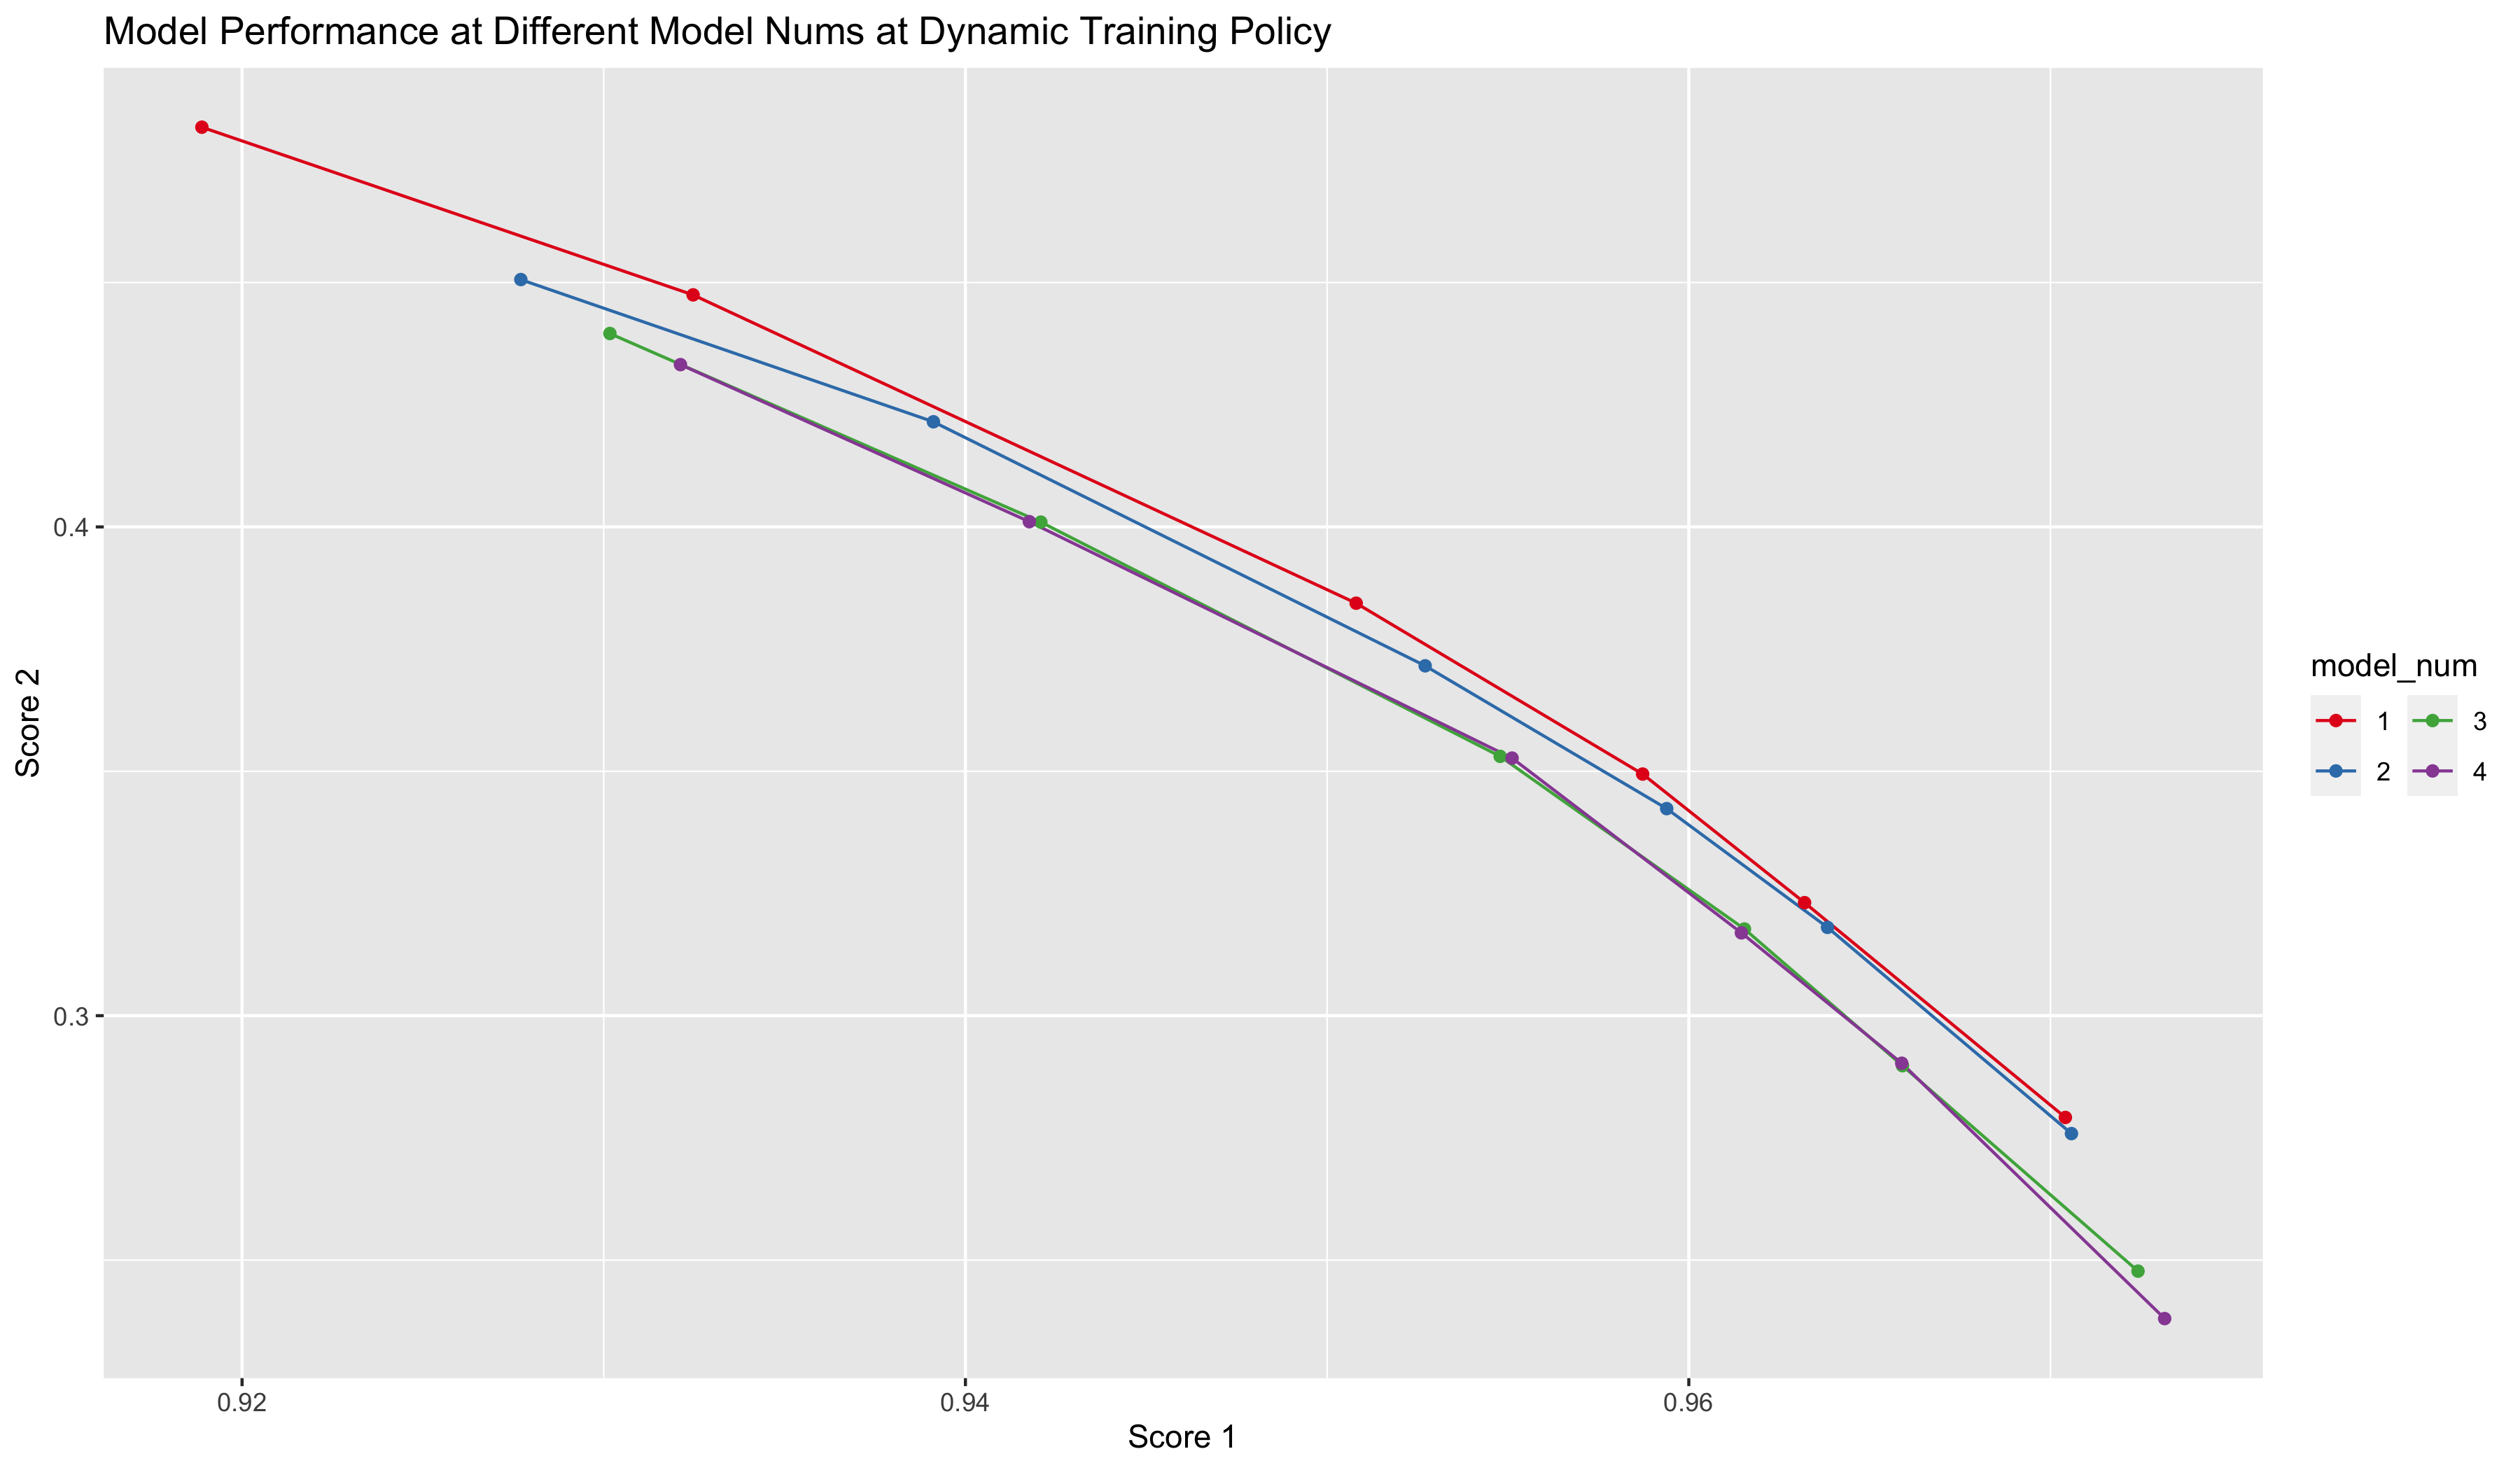
\includegraphics[width = 0.8\textwidth]{images/ModelPerformanceatDifferentModelNumsatDynamicTrainingPolicy.png}
    \label{fig:fig1.6.1}
\end{figure}

\begin{table}[htbp]
  \begin{center}
    \caption{Configuration and Result of AR1 Model with Different Model Number and Dynamic Training}
    \label{tab:tab1.6.1}
    \begin{tabular}{l|l|*{4}{c}} \textbf{model num} & \textbf{cut off prob} &
      \textbf{score 1} & \textbf{score 1 weight} & \textbf{score 2} &
      \textbf{score 2 weight} \\
      \hline
      1 & 0.001 & 0.9704 & 42449 & 0.2792 & 59249\\
      1 & 0.003 & 0.9632 & 45137 & 0.3231 & 59249\\
      1 & 0.005 & 0.9587 & 46419 & 0.3494 & 59249\\
      1 & 0.010 & 0.9508 & 47422 & 0.3844 & 59249\\
      1 & 0.030 & 0.9325 & 50363 & 0.4475 & 59249\\
      1 & 0.050 & 0.9189 & 52866 & 0.4818 & 59249\\
      2 & 0.001 & 0.9706 & 42352 & 0.2759 & 59249\\
      2 & 0.003 & 0.9638 & 44989 & 0.3181 & 59249\\
      2 & 0.005 & 0.9594 & 46071 & 0.3424 & 59249\\
      2 & 0.010 & 0.9527 & 47453 & 0.3716 & 59249\\
      2 & 0.030 & 0.9391 & 49963 & 0.4215 & 59249\\
      2 & 0.050 & 0.9277 & 52260 & 0.4506 & 59249\\
      3 & 0.001 & 0.9724 & 39050 & 0.2477 & 59249\\
      3 & 0.003 & 0.9659 & 42414 & 0.2898 & 59249\\
      3 & 0.005 & 0.9615 & 44330 & 0.3177 & 59249\\
      3 & 0.010 & 0.9548 & 45913 & 0.3531 & 59249\\
      3 & 0.030 & 0.9421 & 48813 & 0.4010 & 59249\\
      3 & 0.050 & 0.9302 & 51368 & 0.4396 & 59249\\
      4 & 0.001 & 0.9732 & 38110 & 0.2380 & 59249\\
      4 & 0.003 & 0.9659 & 42477 & 0.2903 & 59249\\
      4 & 0.005 & 0.9615 & 44285 & 0.3169 & 59249\\
      4 & 0.010 & 0.9551 & 45760 & 0.3527 & 59249\\
      4 & 0.030 & 0.9418 & 48358 & 0.4011 & 59249\\
      4 & 0.050 & 0.9321 & 51371 & 0.4332 & 59249\\
    \end{tabular}
  \end{center}
\end{table}

\begin{figure}
    \caption{An Example Trace with Three Parallel AR1 Models and Offline Training}
    \centering
    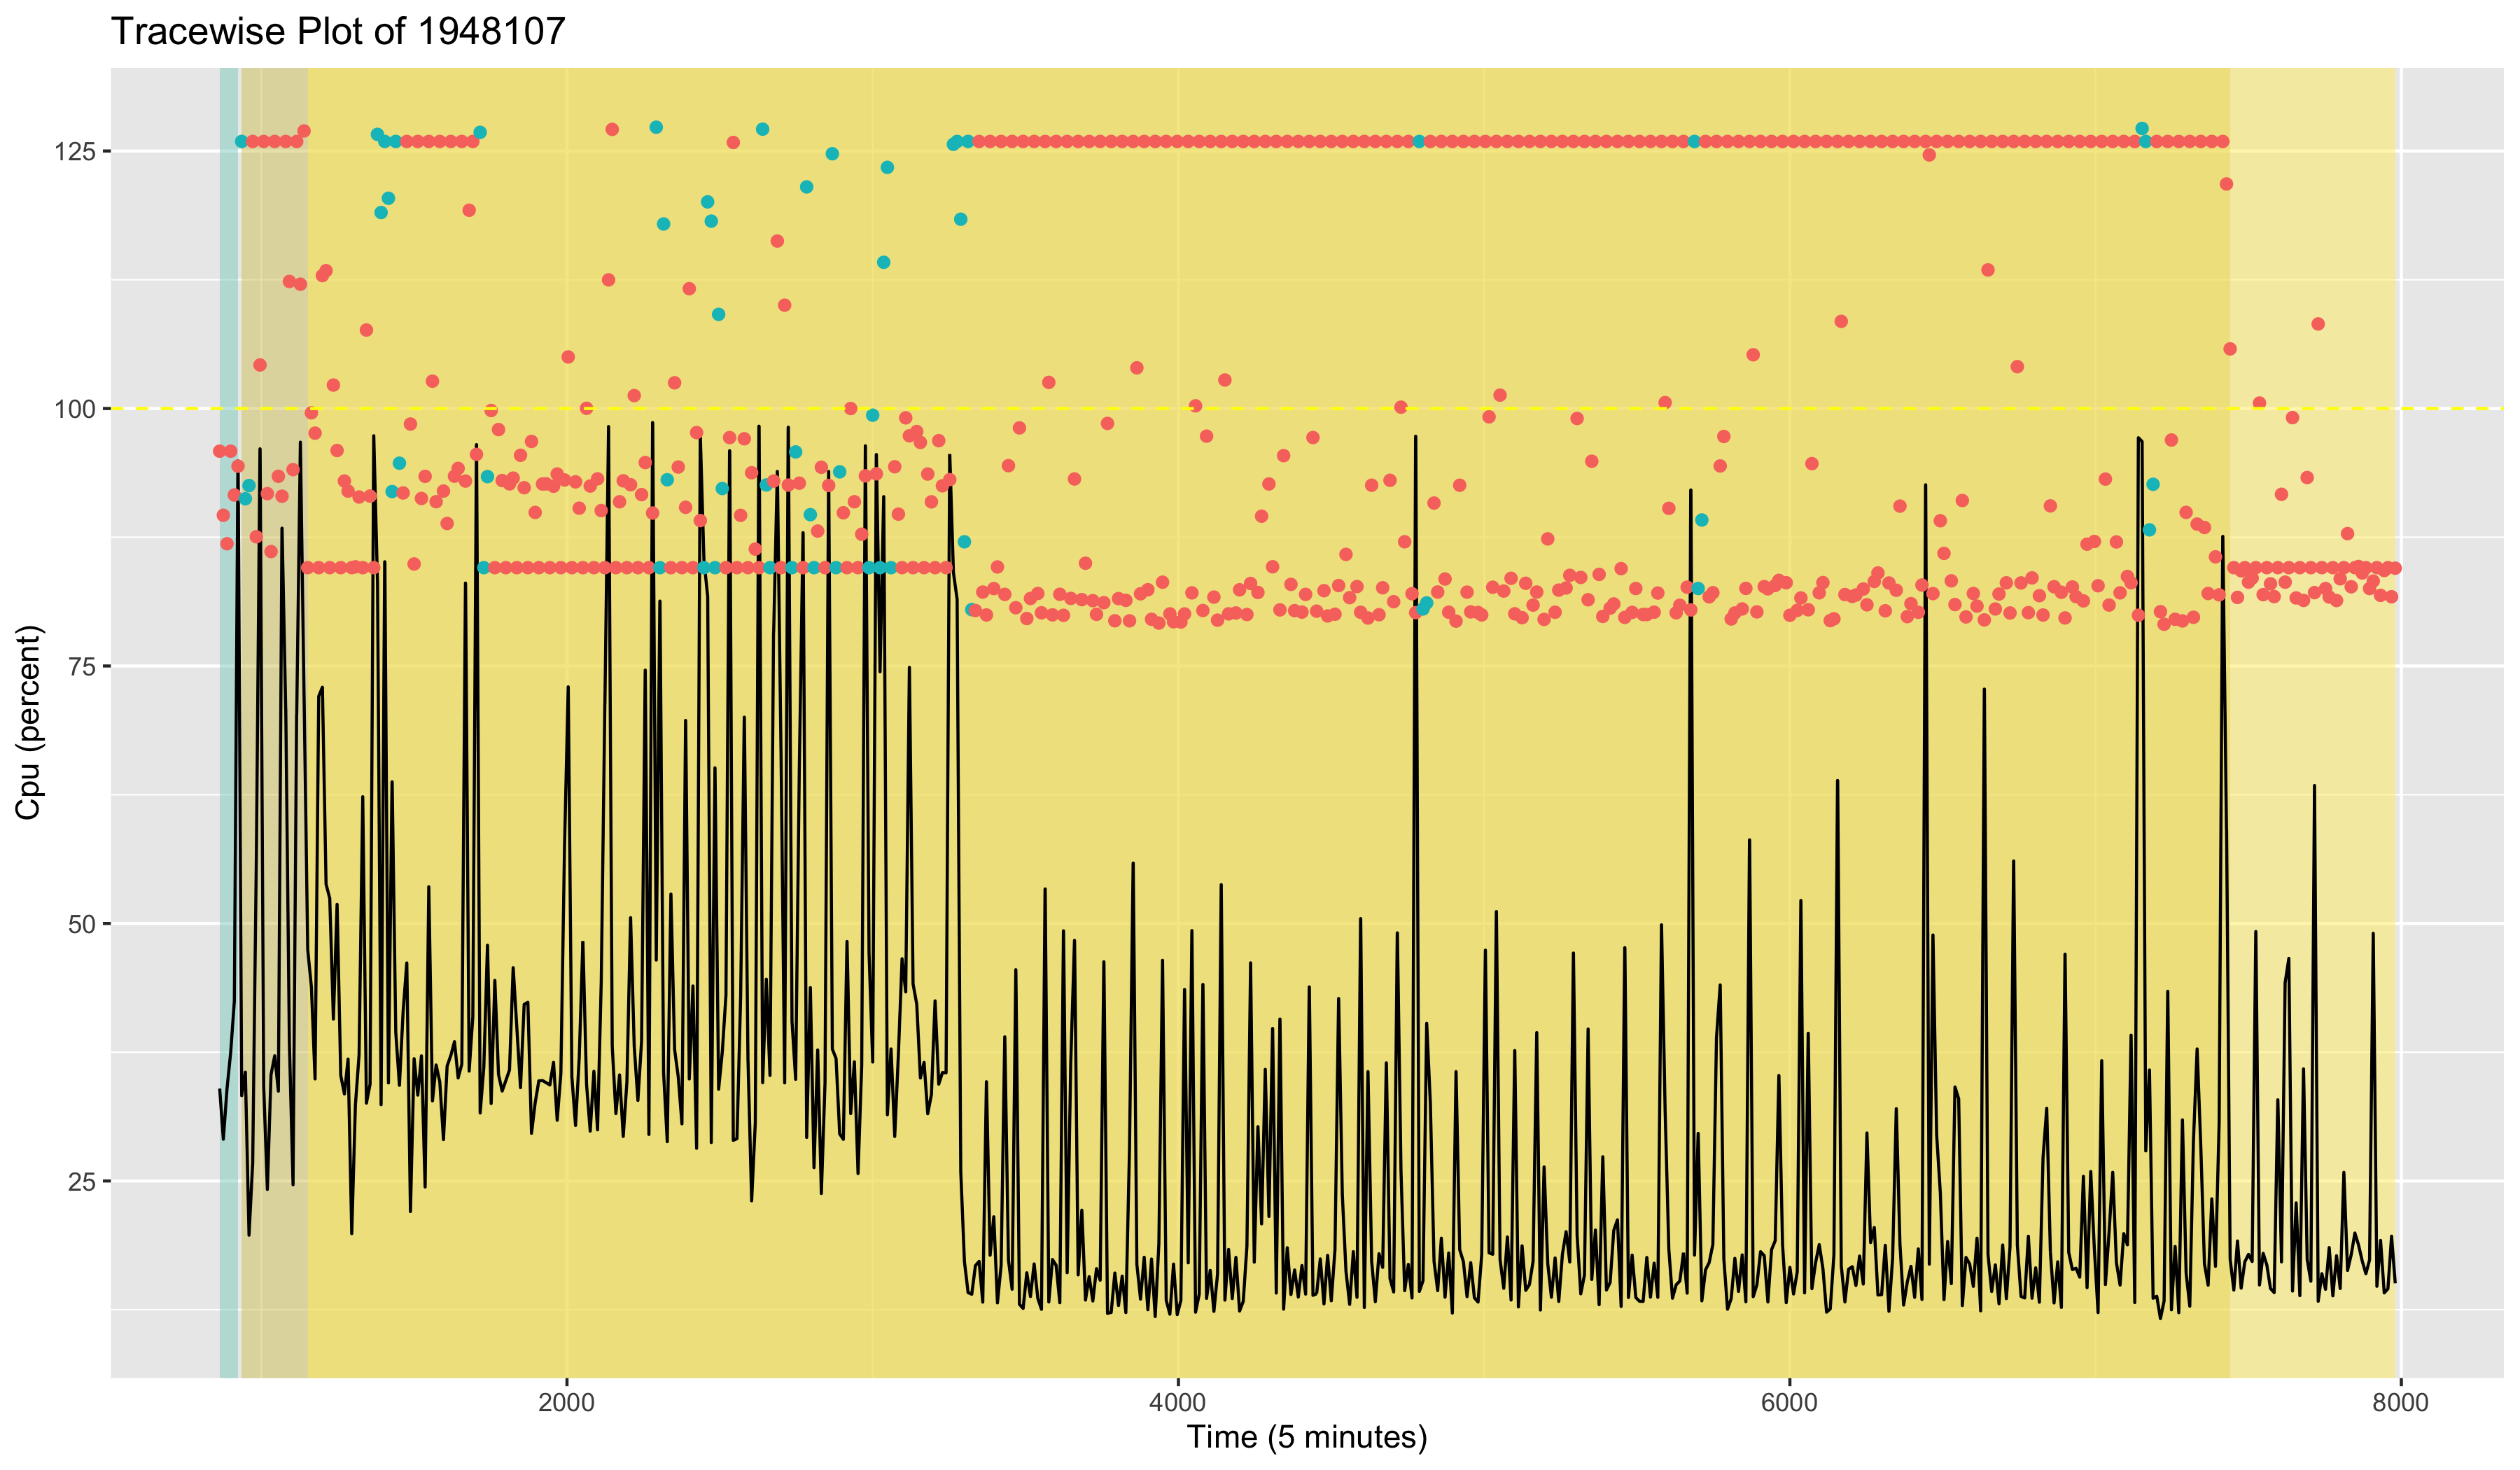
\includegraphics[width = 0.8\textwidth]{images/Tracewise Plot of 1948107, AR1, offline.png}
    \label{fig:fig1.6.2}
\end{figure}

\begin{figure}
    \caption{An Example Trace with Three Parallel AR1 Models and Dynamic Training}
    \centering
    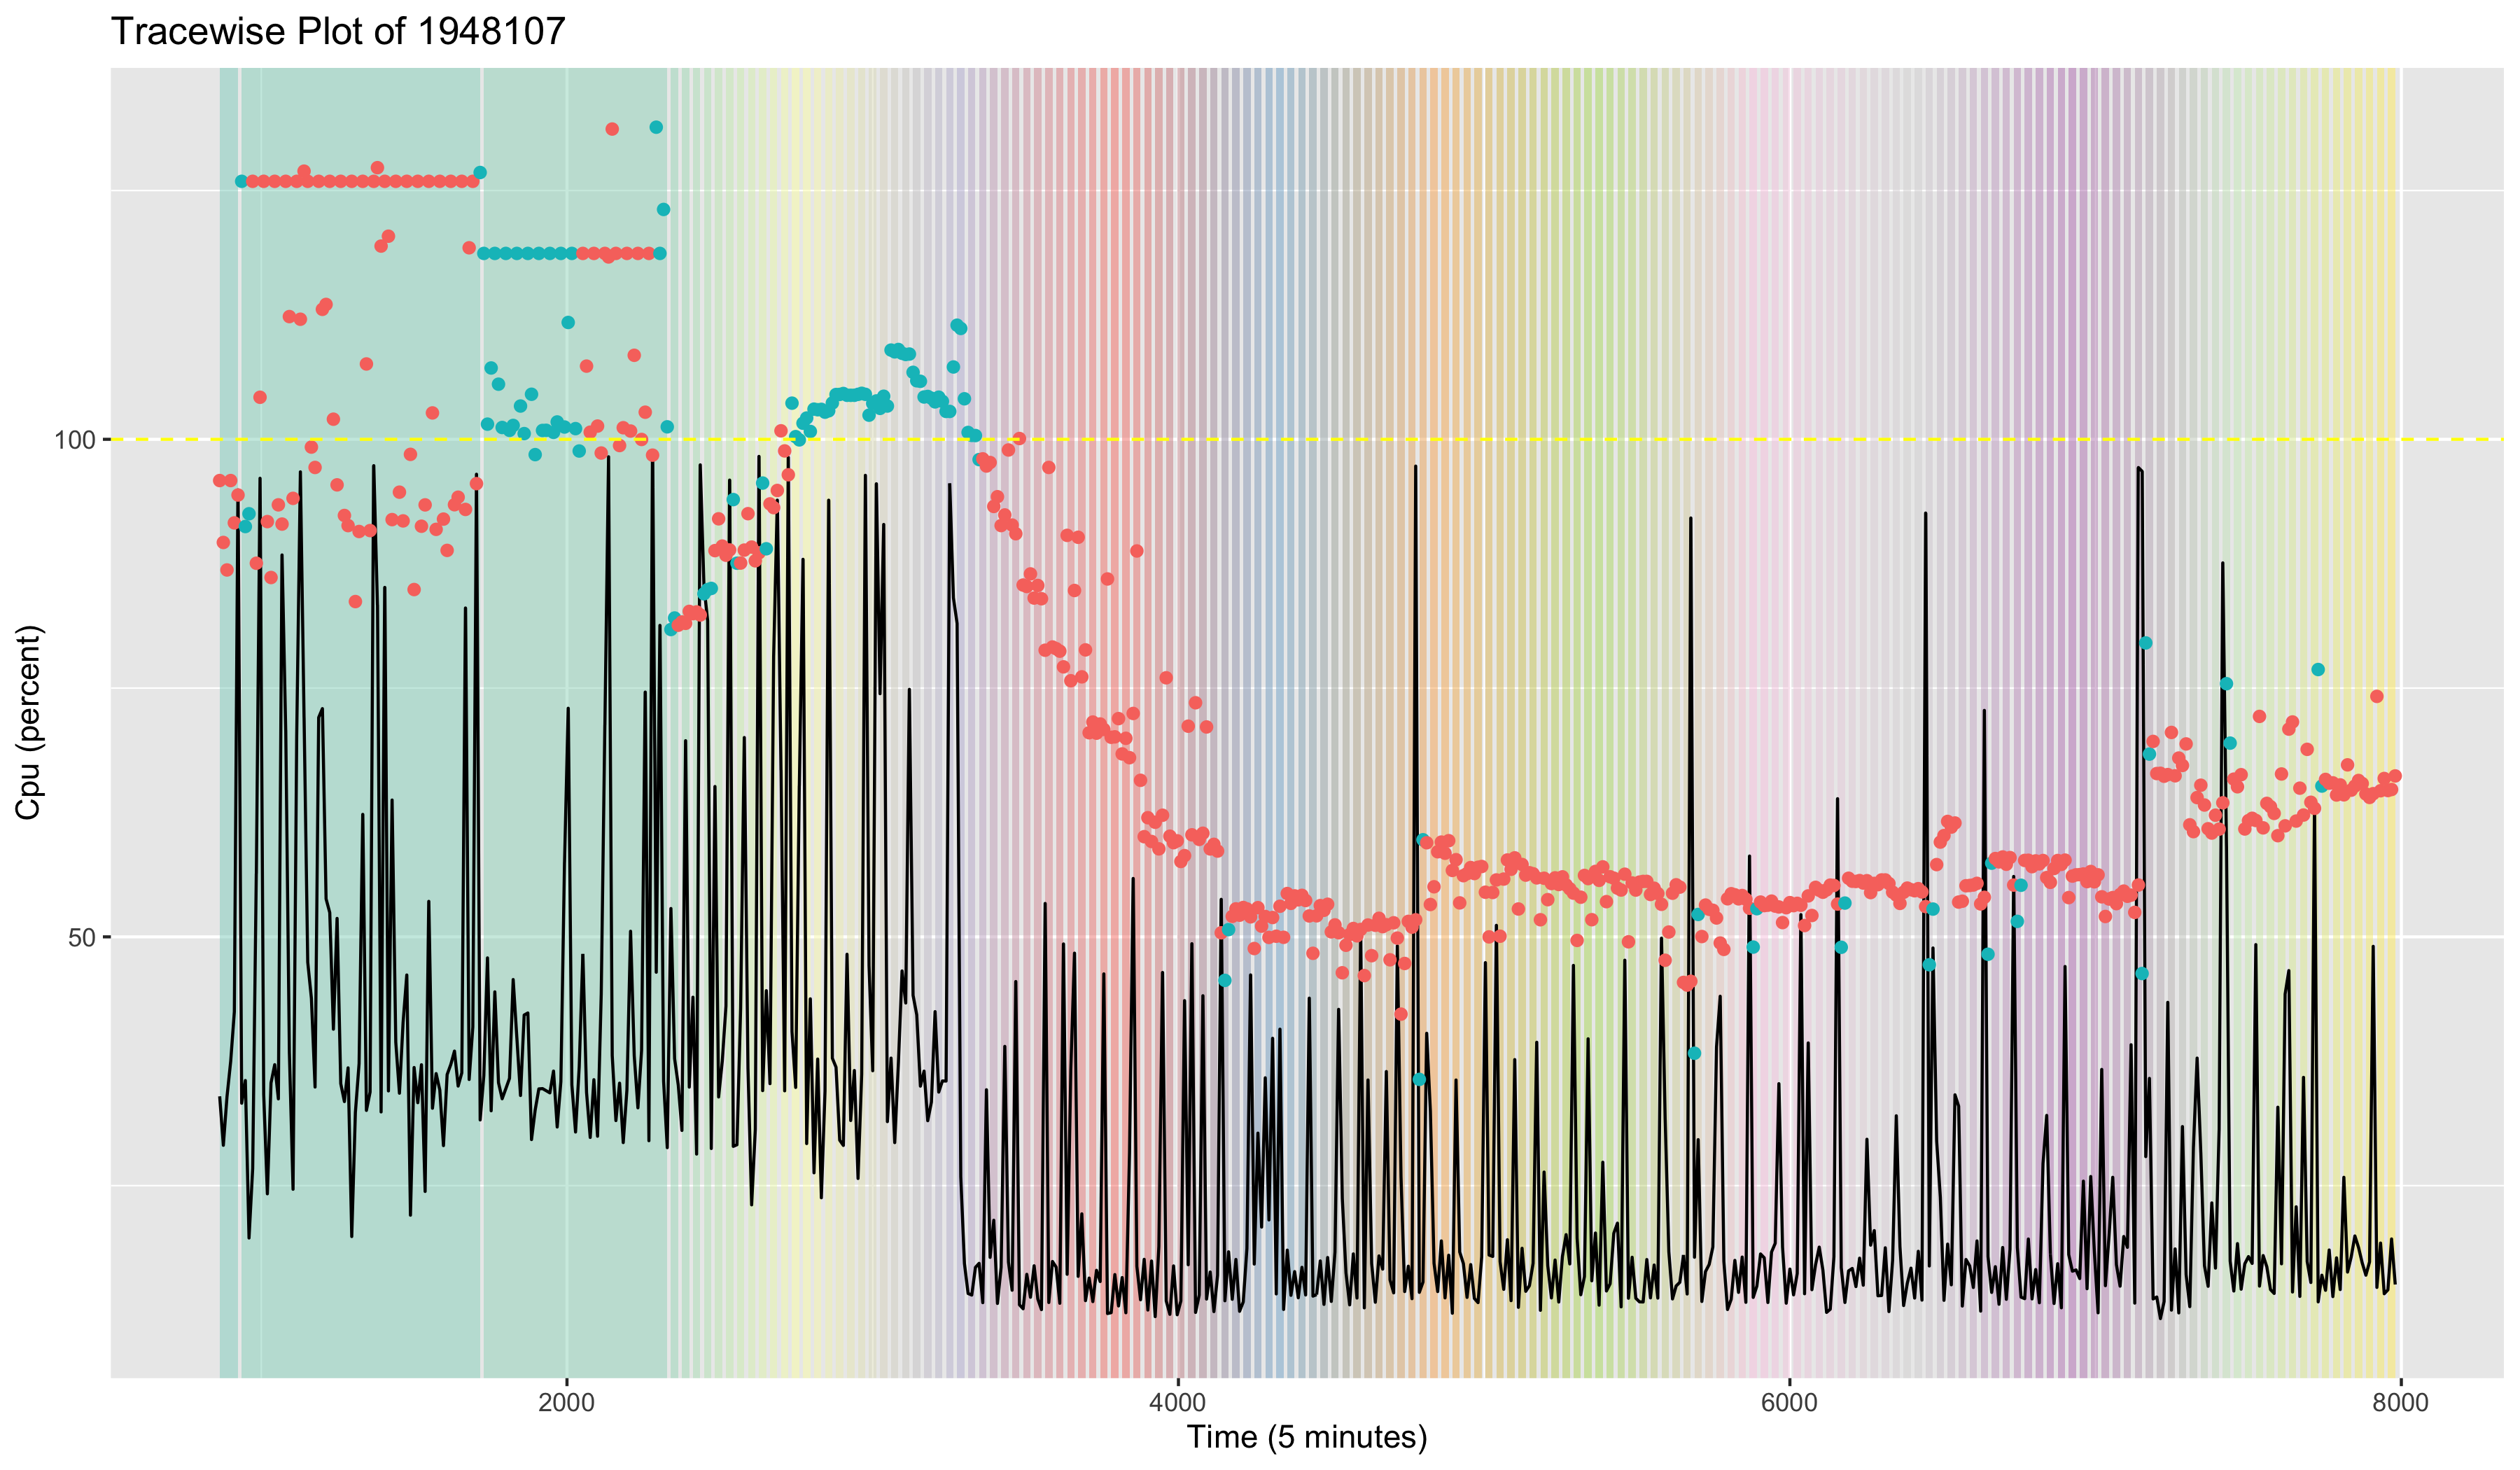
\includegraphics[width = 0.8\textwidth]{images/Tracewise Plot of 1948107, AR1, dynamic.png}
    \label{fig:fig1.6.3}
\end{figure}

\subsubsection{Granularity}
Ref to Section 1.7, include Fig \ref{fig:fig1.7.1}, Table \ref{tab:tab1.7.1}.

\begin{figure}
    \caption{ECDF of Scores for Different Granularity of Offline Training}
    \centering
    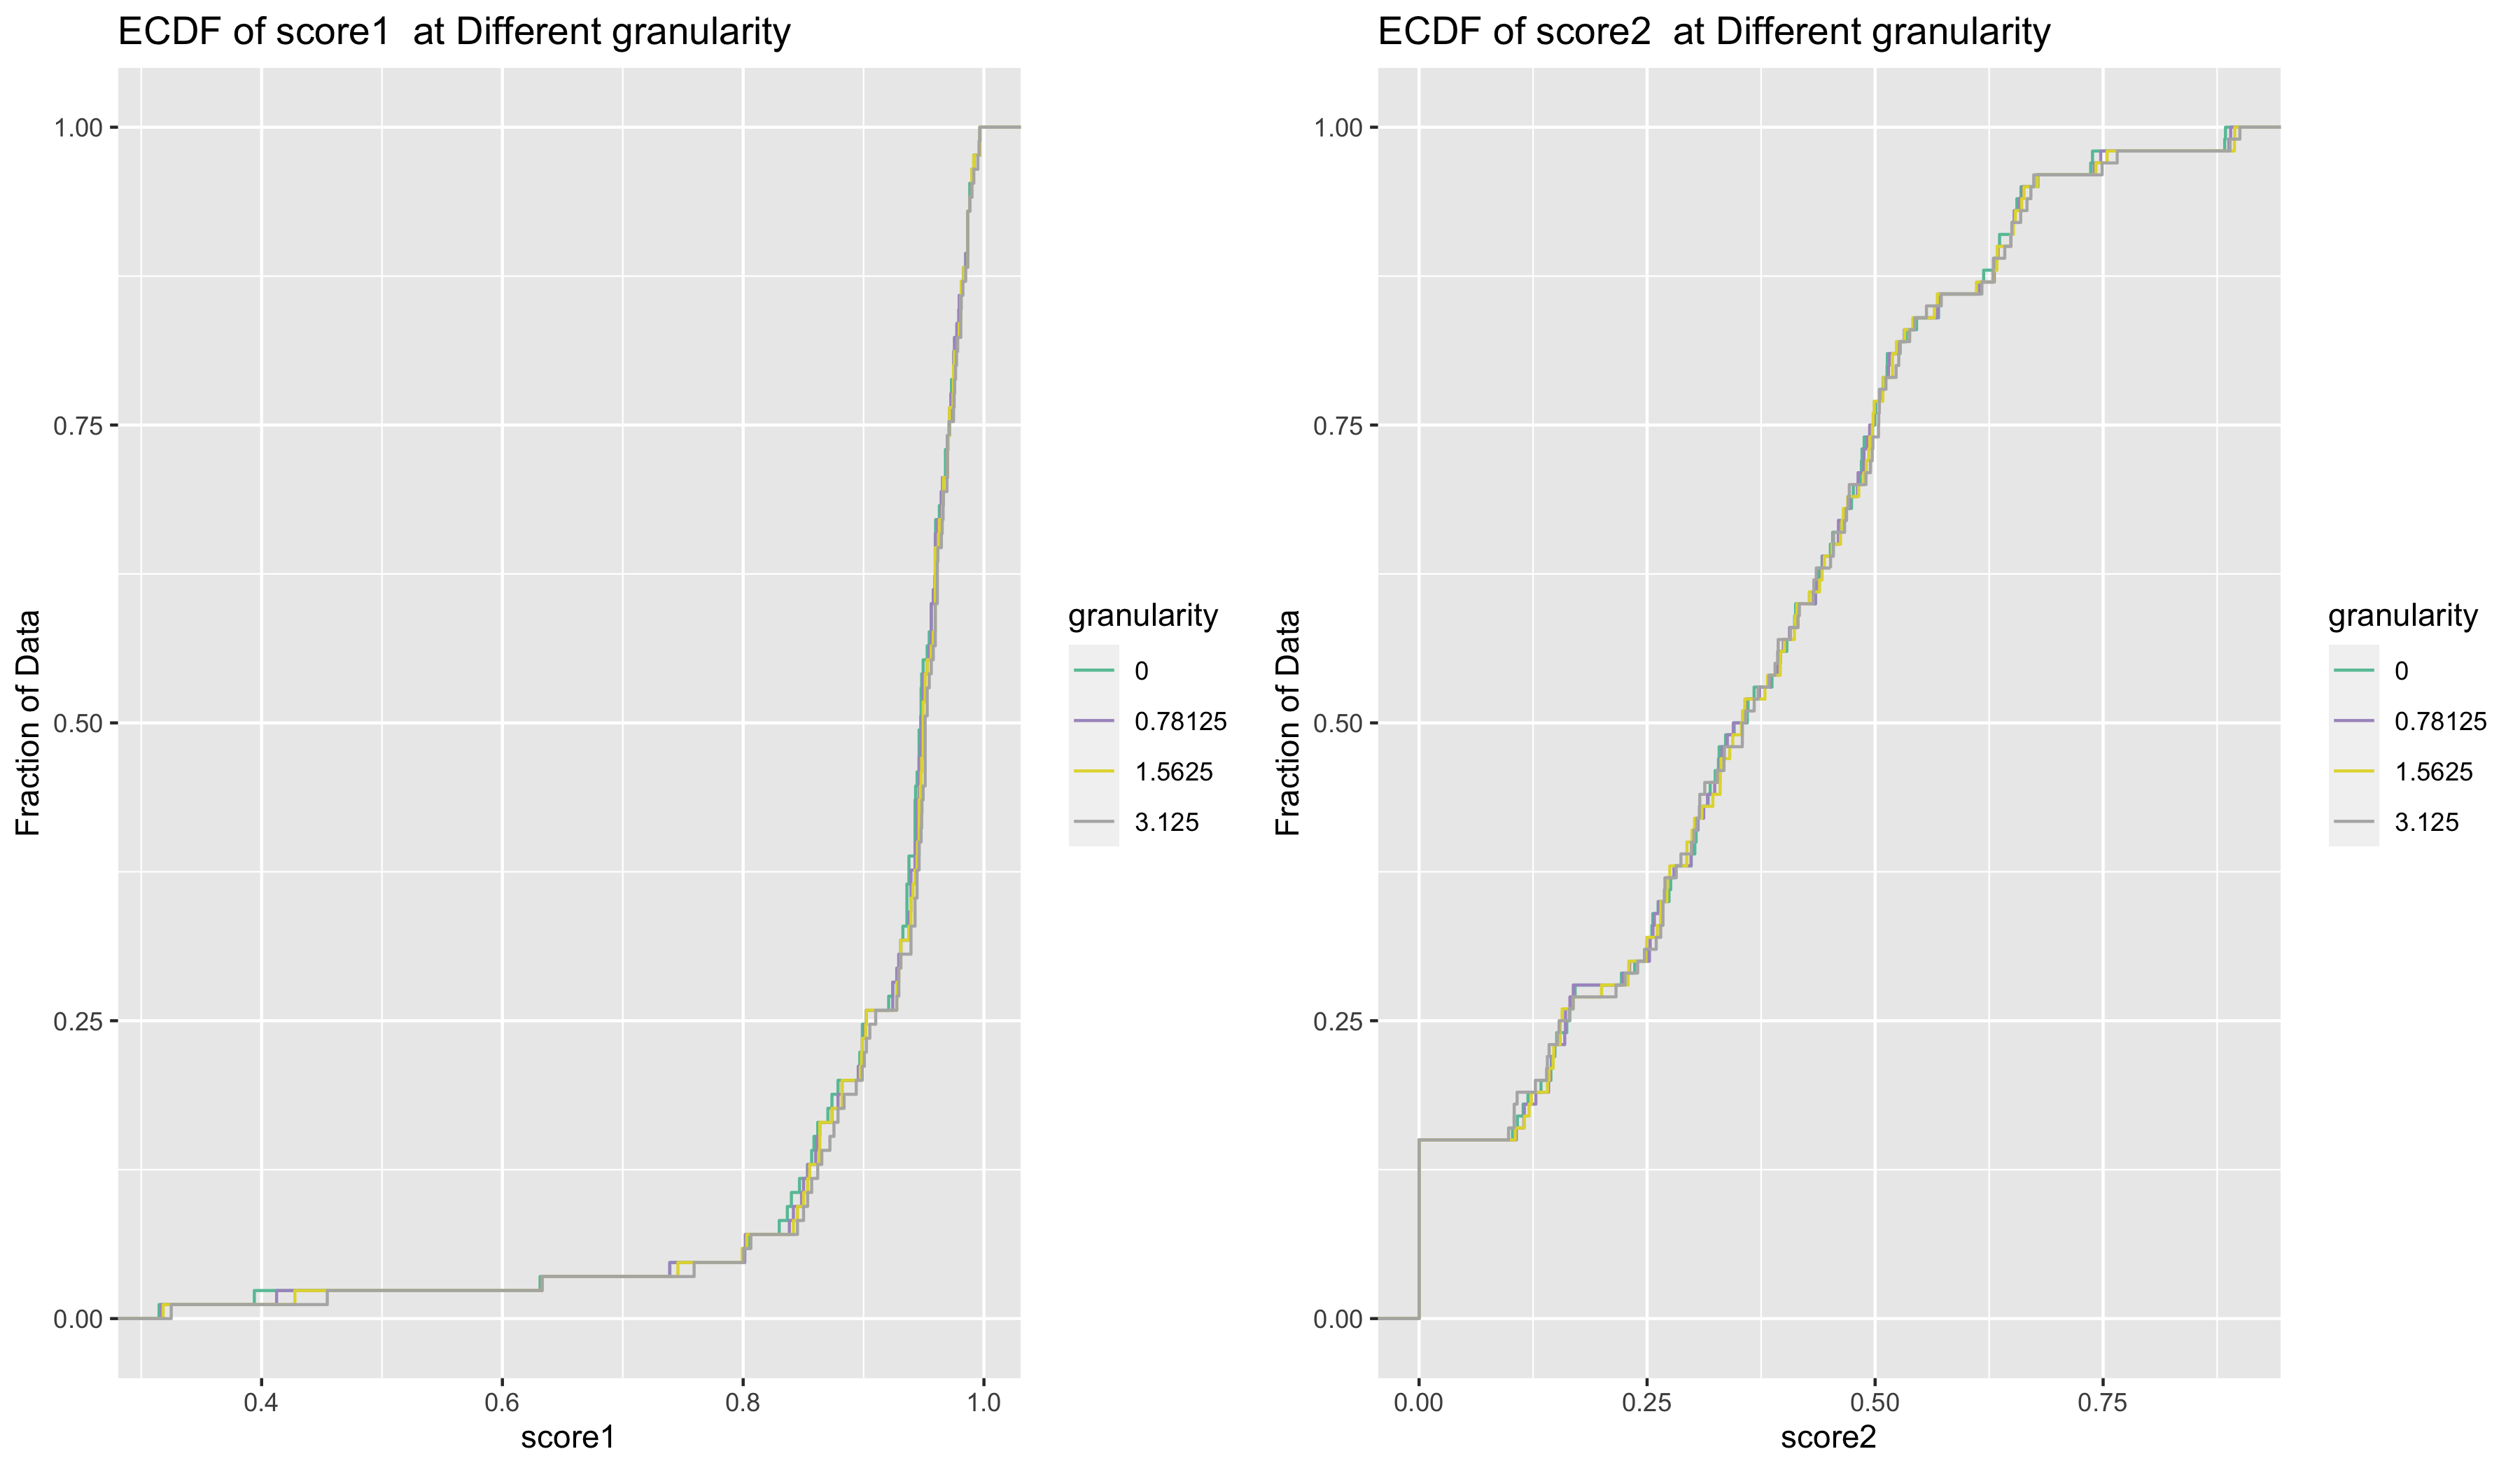
\includegraphics{images/ECDFofscoresatDifferentGranularityOfAR1ModelOfflineTrainingPolicy.png}
    \label{fig:fig1.7.1}
\end{figure}

\begin{table}[htbp]
  \begin{center}
    \caption{Configuration and Result of AR1 Model with Different Granularity and Offline Training}
    \label{tab:tab1.7.1}
    \begin{tabular}{l|*{4}{c}} \textbf{granularity} & \textbf{score 1} &
      \textbf{score 1 weight} & \textbf{score 2} & \textbf{score 2 weight} \\
      \hline
      0.00000 & 0.9168 & 48124 & 0.3463 & 59249\\
      0.78125 & 0.9183 & 48070 & 0.3577 & 57170\\
      1.56250 & 0.9197 & 47992 & 0.3638 & 56005\\
      3.12500 & 0.9224 & 47725 & 0.3667 & 55163\\
    \end{tabular}
  \end{center}
\end{table}

\subsubsection{Adjustment Policy}
Ref to Section 1.8, include Fig \ref{fig:fig1.8.1}, Table \ref{tab:tab1.8.1}.

\begin{figure}
    \caption{Trade-off Curves for Different React Speed of Adjustment Policy of Offline Training}
    \centering
    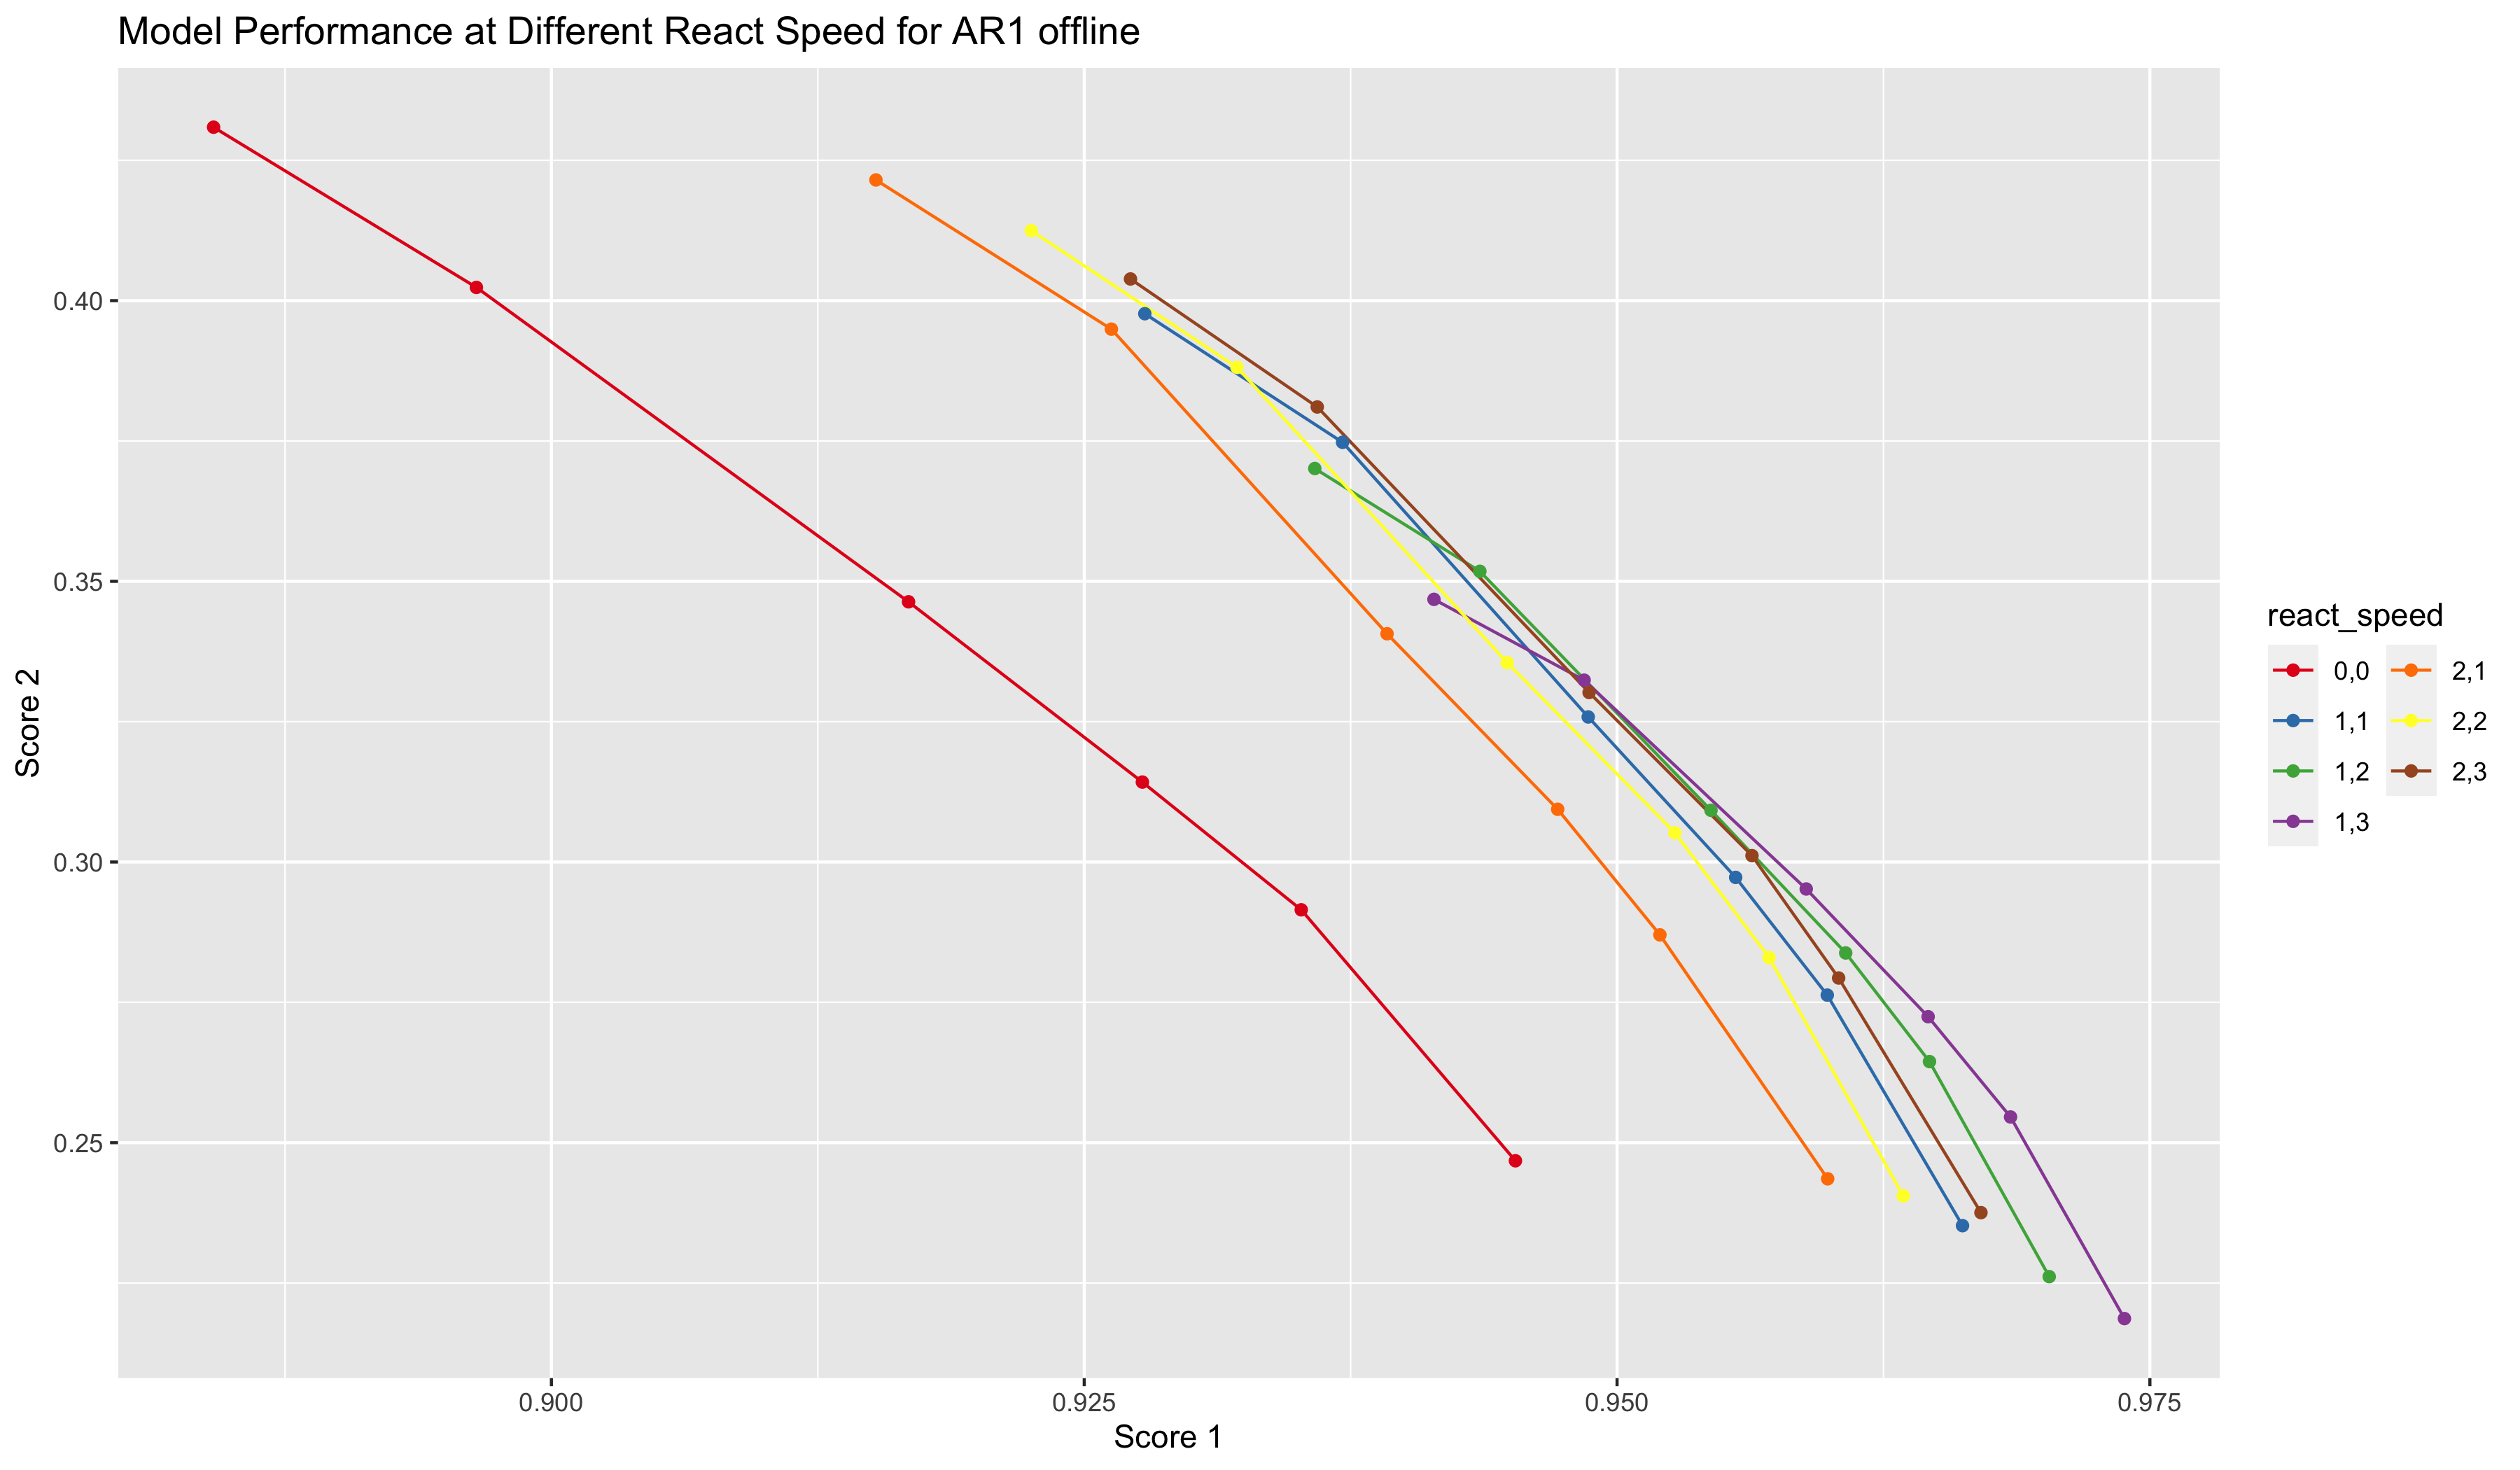
\includegraphics{images/ModelPerformanceatDifferentReactSpeedforAR1offline.png}
    \label{fig:fig1.8.1}
\end{figure}

\begin{longtable}[htbp]{l|l|l|*{4}{c}}
    \caption{Configuration and Result of AR1 Model with Different React Speed of Adjustment Policy of Offline Training}
    \label{tab:tab1.8.1} \\
    \textbf{react speed} & \textbf{cut off prob} & \textbf{score 1} &
    \textbf{score 1 weight} & \textbf{score 2} & \textbf{score 2 weight} \\
    \hline
    0,0 & 0.9452 & 42981 & 0.2468 & 59249\\
    0,0 & 0.9352 & 46484 & 0.2915 & 59249\\
    0,0 & 0.9277 & 47487 & 0.3142 & 59249\\
    0,0 & 0.9168 & 48124 & 0.3463 & 59249\\
    0,0 & 0.8965 & 50300 & 0.4024 & 59249\\
    0,0 & 0.8841 & 52904 & 0.4309 & 59249\\
    1,1 & 0.9662 & 40631 & 0.2352 & 59249\\
    1,1 & 0.9599 & 43476 & 0.2763 & 59249\\
    1,1 & 0.9556 & 44064 & 0.2973 & 59249\\
    1,1 & 0.9486 & 44126 & 0.3258 & 59249\\
    1,1 & 0.9371 & 45102 & 0.3748 & 59249\\
    1,1 & 0.9278 & 46786 & 0.3977 & 59249\\
    1,2 & 0.9703 & 39262 & 0.2261 & 59249\\
    1,2 & 0.9647 & 41736 & 0.2644 & 59249\\
    1,2 & 0.9607 & 42116 & 0.2838 & 59249\\
    1,2 & 0.9544 & 41871 & 0.3092 & 59249\\
    1,2 & 0.9436 & 42277 & 0.3518 & 59249\\
    1,2 & 0.9358 & 43423 & 0.3701 & 59249\\
    1,3 & 0.9738 & 38100 & 0.2187 & 59249\\
    1,3 & 0.9685 & 40269 & 0.2546 & 59249\\
    1,3 & 0.9646 & 40475 & 0.2724 & 59249\\
    1,3 & 0.9589 & 39976 & 0.2952 & 59249\\
    1,3 & 0.9485 & 39907 & 0.3324 & 59249\\
    1,3 & 0.9414 & 40655 & 0.3468 & 59249\\
    1,3 & 0.9599 & 42001 & 0.2436 & 59249\\
    1,3 & 0.9520 & 45218 & 0.2870 & 59249\\
    1,3 & 0.9472 & 46016 & 0.3094 & 59249\\
    1,3 & 0.9392 & 46387 & 0.3407 & 59249\\
    1,3 & 0.9263 & 47934 & 0.3949 & 59249\\
    1,3 & 0.9152 & 50157 & 0.4215 & 59249\\
    2,2 & 0.9634 & 41534 & 0.2405 & 59249\\
    2,2 & 0.9571 & 44556 & 0.2830 & 59249\\
    2,2 & 0.9527 & 45297 & 0.3052 & 59249\\
    2,2 & 0.9448 & 45564 & 0.3355 & 59249\\
    2,2 & 0.9322 & 46940 & 0.3881 & 59249\\
    2,2 & 0.9225 & 48861 & 0.4125 & 59249\\
    2,3 & 0.9671 & 41031 & 0.2375 & 59249\\
    2,3 & 0.9604 & 43986 & 0.2793 & 59249\\
    2,3 & 0.9563 & 44653 & 0.3011 & 59249\\
    2,3 & 0.9487 & 44804 & 0.3302 & 59249\\
    2,3 & 0.9359 & 46030 & 0.3811 & 59249\\
    2,3 & 0.9272 & 47755 & 0.4039 & 59249\\
\end{longtable}

\begin{figure}
    \caption{Trade-off Curves for Different React Speed of Adjustment Policy of Offline Training}
    \centering
    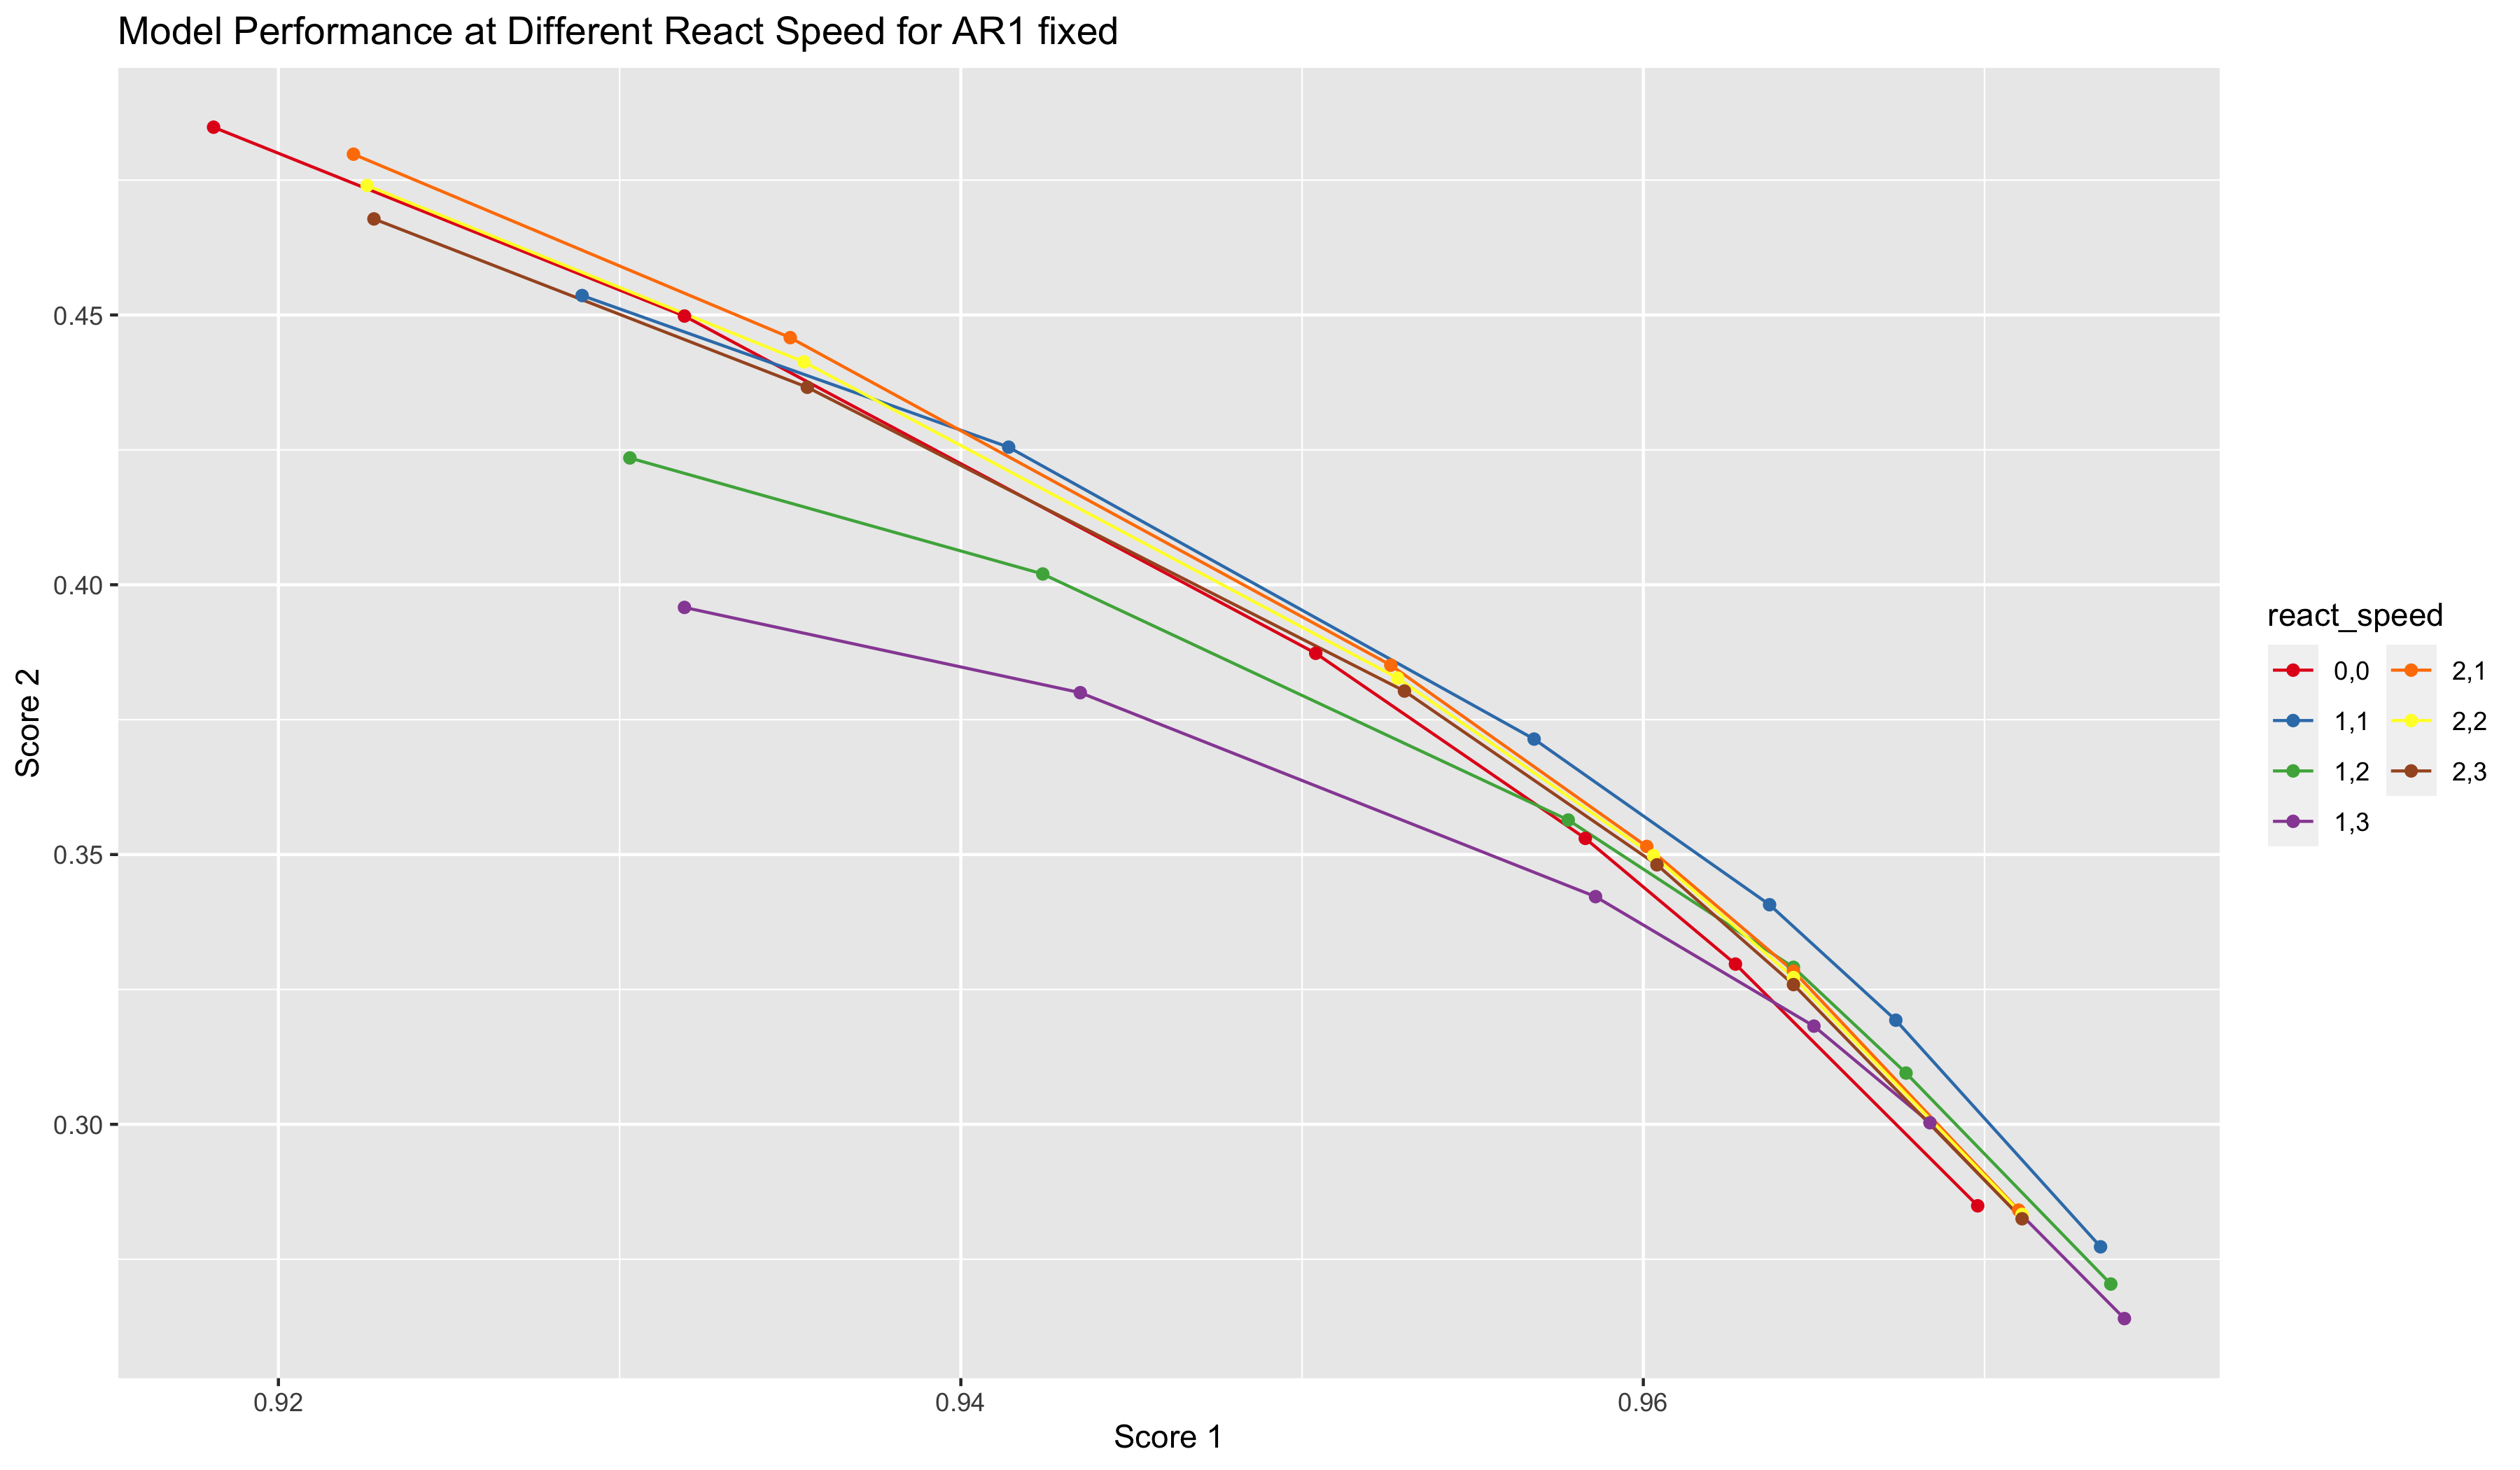
\includegraphics{images/ModelPerformanceatDifferentReactSpeedforAR1fixed.png}
    \label{fig:fig1.8.2}
\end{figure}

\begin{longtable}[htbp]{l|l|l|*{4}{c}}
    \caption{Configuration and Result of AR1 Model with Different React Speed of Adjustment Policy of Fixed Point Training}
    \label{tab:tab1.8.2} \\
    \textbf{react speed} & \textbf{cut off prob} & \textbf{score 1} &
    \textbf{score 1 weight} & \textbf{score 2} & \textbf{score 2 weight} \\
    \hline
    0,0 & 0.001 & 0.9698 & 42245 & 0.2849 & 59249\\
    0,0 & 0.003 & 0.9627 & 45239 & 0.3297 & 59249\\
    0,0 & 0.005 & 0.9583 & 46435 & 0.3530 & 59249\\
    0,0 & 0.010 & 0.9504 & 47518 & 0.3873 & 59249\\
    0,0 & 0.030 & 0.9319 & 50406 & 0.4498 & 59249\\
    0,0 & 0.050 & 0.9181 & 52841 & 0.4848 & 59249\\
    1,1 & 0.001 & 0.9734 & 40973 & 0.2773 & 59249\\
    1,1 & 0.003 & 0.9674 & 43557 & 0.3193 & 59249\\
    1,1 & 0.005 & 0.9637 & 44503 & 0.3407 & 59249\\
    1,1 & 0.010 & 0.9568 & 45166 & 0.3714 & 59249\\
    1,1 & 0.030 & 0.9414 & 46979 & 0.4255 & 59249\\
    1,1 & 0.050 & 0.9289 & 48523 & 0.4536 & 59249\\
    1,2 & 0.001 & 0.9737 & 39888 & 0.2704 & 59249\\
    1,2 & 0.003 & 0.9677 & 42141 & 0.3095 & 59249\\
    1,2 & 0.005 & 0.9644 & 42896 & 0.3291 & 59249\\
    1,2 & 0.010 & 0.9578 & 43223 & 0.3564 & 59249\\
    1,2 & 0.030 & 0.9424 & 44234 & 0.4020 & 59249\\
    1,2 & 0.050 & 0.9303 & 45085 & 0.4235 & 59249\\
    1,3 & 0.001 & 0.9741 & 38844 & 0.2640 & 59249\\
    1,3 & 0.003 & 0.9684 & 40789 & 0.3003 & 59249\\
    1,3 & 0.005 & 0.9650 & 41381 & 0.3182 & 59249\\
    1,3 & 0.010 & 0.9586 & 41407 & 0.3422 & 59249\\
    1,3 & 0.030 & 0.9435 & 41700 & 0.3800 & 59249\\
    1,3 & 0.050 & 0.9319 & 41960 & 0.3958 & 59249\\
    2,1 & 0.001 & 0.9710 & 42061 & 0.2841 & 59249\\
    2,1 & 0.003 & 0.9644 & 44974 & 0.3284 & 59249\\
    2,1 & 0.005 & 0.9601 & 46115 & 0.3515 & 59249\\
    2,1 & 0.010 & 0.9526 & 47112 & 0.3851 & 59249\\
    2,1 & 0.030 & 0.9350 & 49732 & 0.4458 & 59249\\
    2,1 & 0.050 & 0.9222 & 51969 & 0.4798 & 59249\\
    2,2 & 0.001 & 0.9711 & 41919 & 0.2833 & 59249\\
    2,2 & 0.003 & 0.9644 & 44780 & 0.3272 & 59249\\
    2,2 & 0.005 & 0.9603 & 45864 & 0.3498 & 59249\\
    2,2 & 0.010 & 0.9528 & 46782 & 0.3827 & 59249\\
    2,2 & 0.030 & 0.9354 & 49175 & 0.4413 & 59249\\
    2,2 & 0.050 & 0.9226 & 51282 & 0.4740 & 59249\\
    2,3 & 0.001 & 0.9711 & 41775 & 0.2825 & 59249\\
    2,3 & 0.003 & 0.9644 & 44577 & 0.3259 & 59249\\
    2,3 & 0.005 & 0.9604 & 45609 & 0.3481 & 59249\\
    2,3 & 0.010 & 0.9530 & 46446 & 0.3803 & 59249\\
    2,3 & 0.030 & 0.9355 & 48610 & 0.4366 & 59249\\
    2,3 & 0.050 & 0.9228 & 50560 & 0.4678 & 59249\\
\end{longtable}

\subsubsection{Predicting Average of Next Window}
Ref to Section 1.10, include Fig \ref{fig:fig1.10.1}, Table \ref{fig:fig1.10.1}.

\begin{figure}
    \caption{}
    \centering
    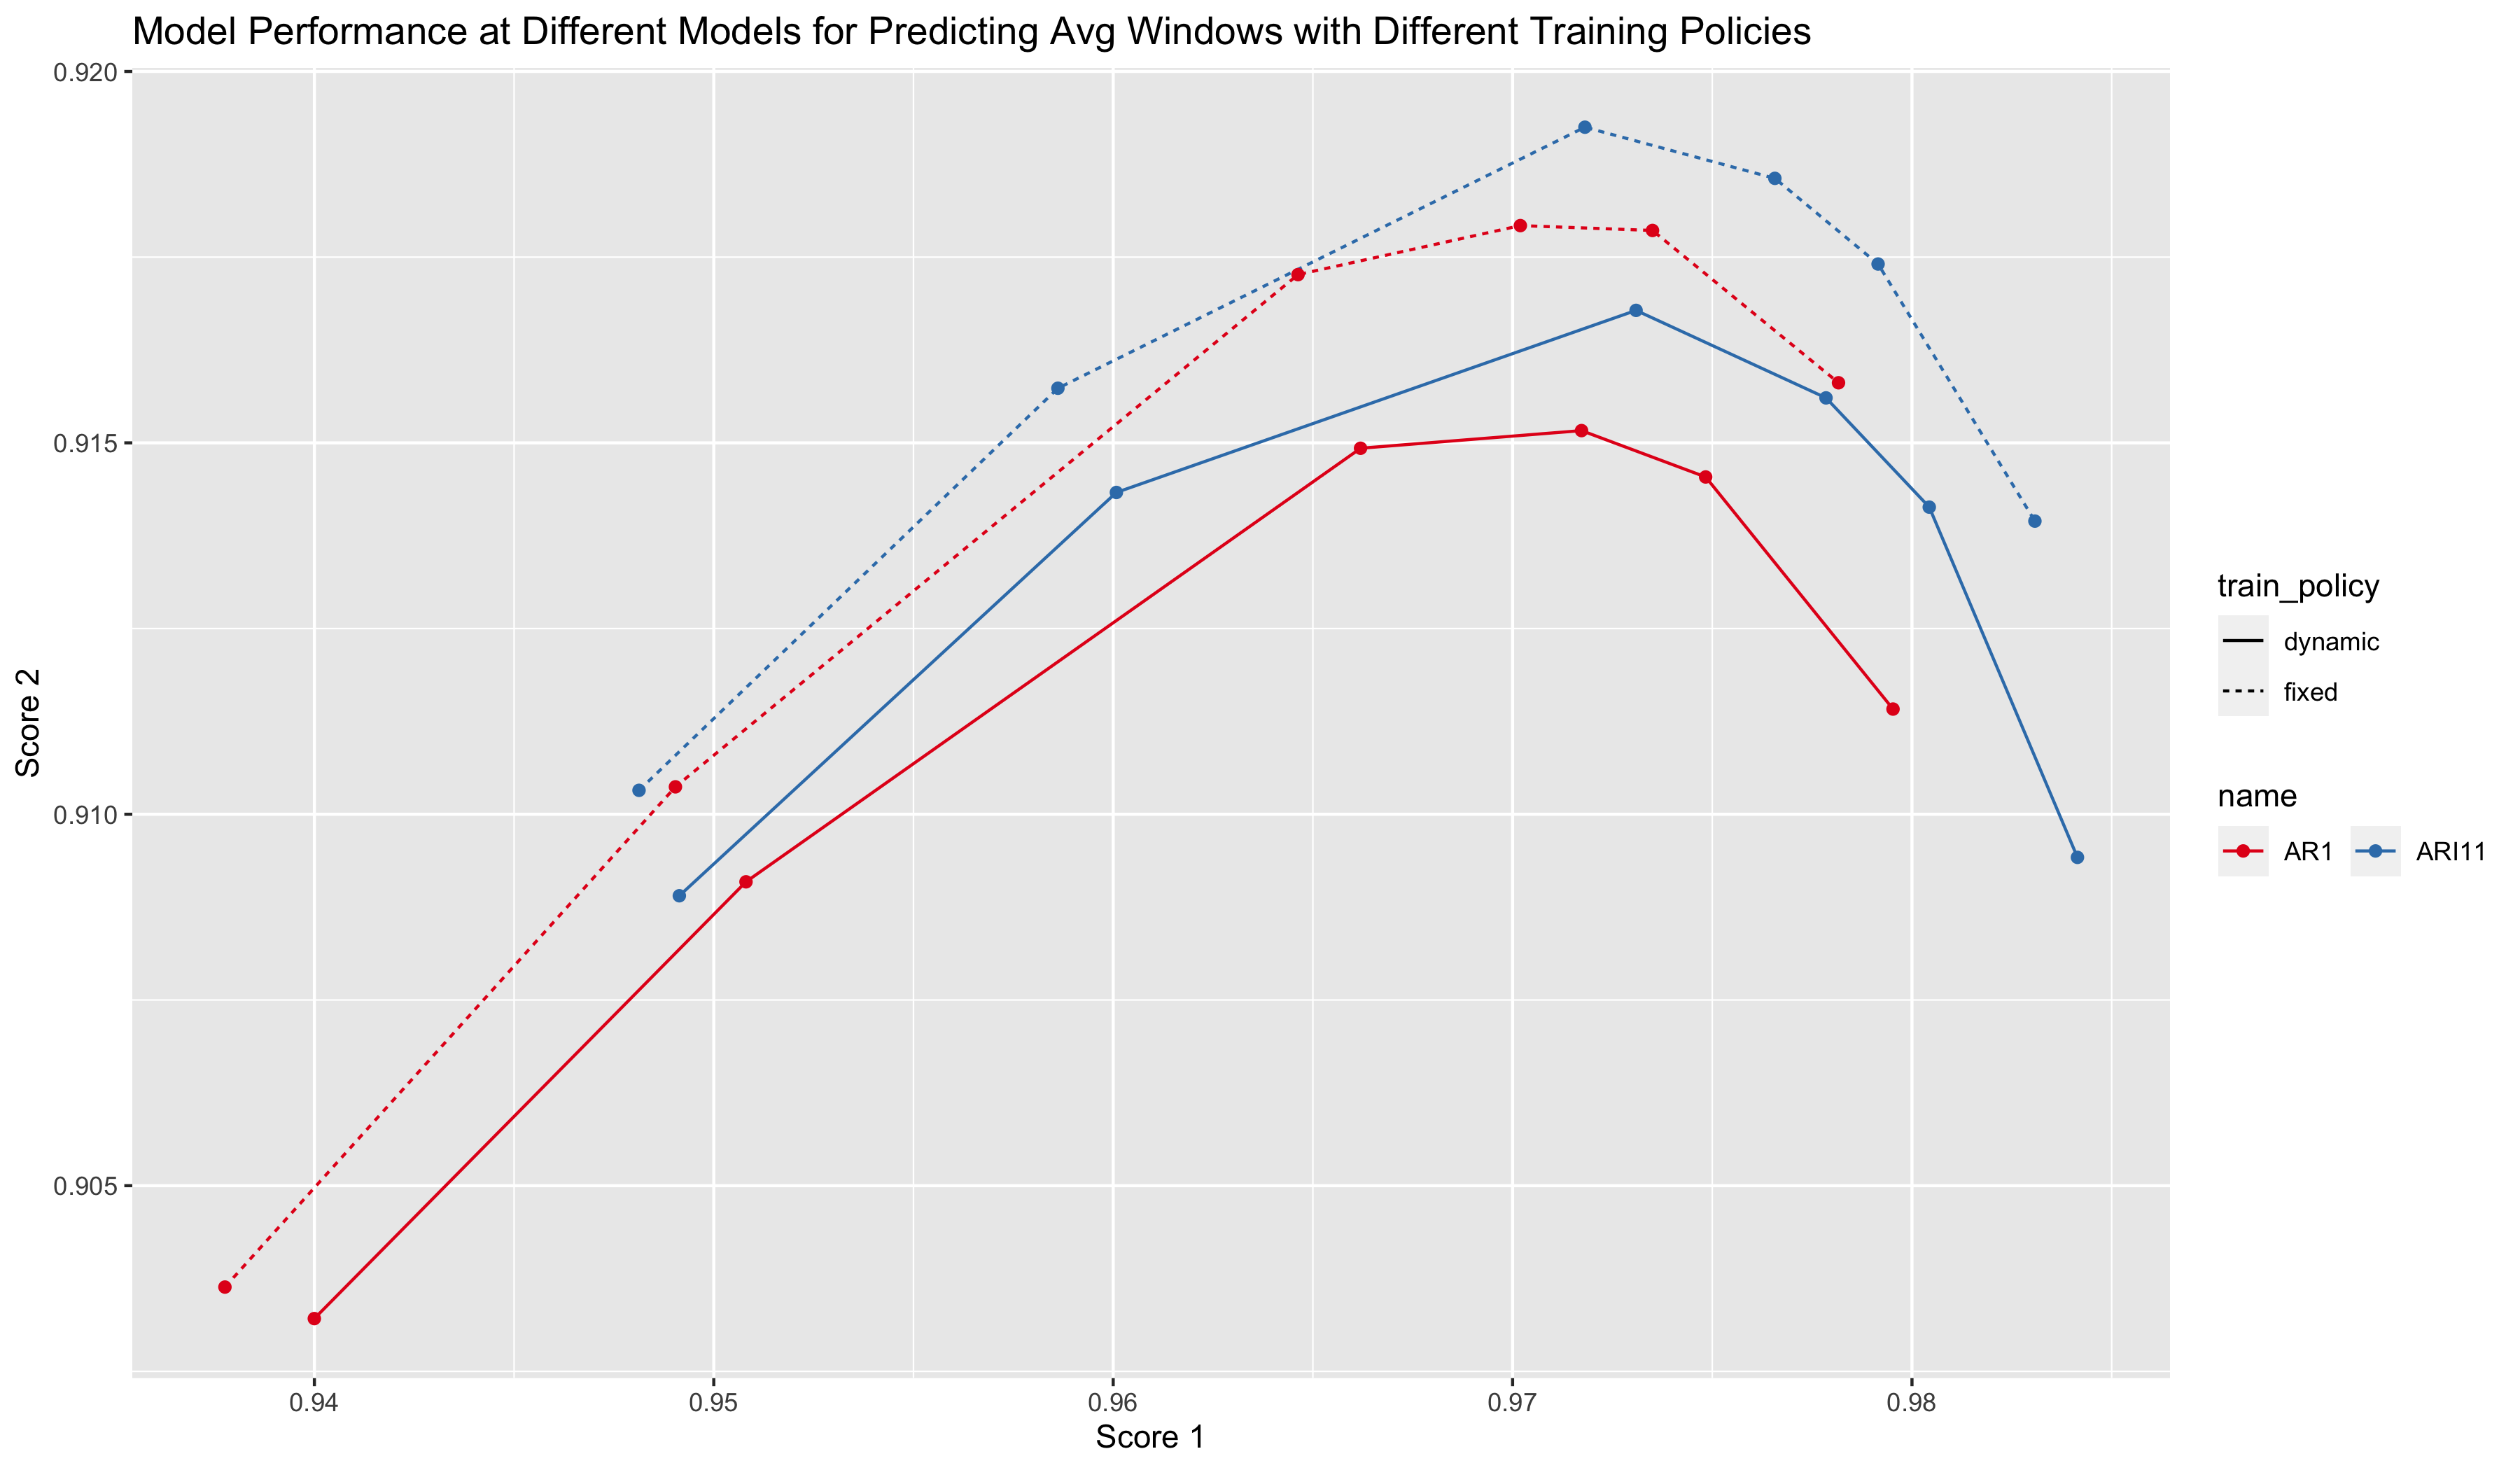
\includegraphics{images/ModelPerformanceatDifferentModelsforPredictingAvgWindowswithDifferentTrainingPolicies.png}
    \label{fig:fig1.10.1}
\end{figure}

\begin{table}[htbp]
  \begin{center}
    \caption{Configuration and Result of Different Models Predicting Averages of Next Window with Offline Training}
    \label{tab:tab1.10.1}
    \begin{tabular}{l|l|l|*{4}{c}} \textbf{model} & \textbf{training policy} &
      \textbf{cut off prob} & \textbf{score 1} & \textbf{score 1 weight} &
      \textbf{score 2} & \textbf{score 2 weight} \\
      \hline
      AR1 & dynamic & 0.001 & 0.9795 & 59341 & 0.9114 & 59400\\
      AR1 & dynamic & 0.003 & 0.9748 & 59365 & 0.9145 & 59400\\
      AR1 & dynamic & 0.005 & 0.9717 & 59384 & 0.9152 & 59400\\
      AR1 & dynamic & 0.010 & 0.9662 & 59397 & 0.9149 & 59400\\
      AR1 & dynamic & 0.030 & 0.9508 & 59398 & 0.9091 & 59400\\
      AR1 & dynamic & 0.050 & 0.9400 & 59398 & 0.9032 & 59400\\
      AR1 & fixed & 0.001 & 0.9782 & 59342 & 0.9158 & 59400\\
      AR1 & fixed & 0.003 & 0.9735 & 59366 & 0.9179 & 59400\\
      AR1 & fixed & 0.005 & 0.9702 & 59385 & 0.9179 & 59400\\
      AR1 & fixed & 0.010 & 0.9646 & 59398 & 0.9173 & 59400\\
      AR1 & fixed & 0.030 & 0.9490 & 59399 & 0.9104 & 59400\\
      AR1 & fixed & 0.050 & 0.9378 & 59399 & 0.9036 & 59400\\
      ARI11 & dynamic & 0.001 & 0.9841 & 59280 & 0.9094 & 59400\\
      ARI11 & dynamic & 0.003 & 0.9804 & 59334 & 0.9141 & 59400\\
      ARI11 & dynamic & 0.005 & 0.9778 & 59361 & 0.9156 & 59400\\
      ARI11 & dynamic & 0.010 & 0.9731 & 59387 & 0.9168 & 59400\\
      ARI11 & dynamic & 0.030 & 0.9601 & 59394 & 0.9143 & 59400\\
      ARI11 & dynamic & 0.050 & 0.9491 & 59395 & 0.9089 & 59400\\
      ARI11 & fixed & 0.001 & 0.9831 & 59271 & 0.9139 & 59400\\
      ARI11 & fixed & 0.003 & 0.9792 & 59332 & 0.9174 & 59400\\
      ARI11 & fixed & 0.005 & 0.9766 & 59360 & 0.9186 & 59400\\
      ARI11 & fixed & 0.010 & 0.9718 & 59386 & 0.9192 & 59400\\
      ARI11 & fixed & 0.030 & 0.9586 & 59395 & 0.9157 & 59400\\
      ARI11 & fixed & 0.050 & 0.9481 & 59396 & 0.9103 & 59400\\
    \end{tabular}
  \end{center}
\end{table}

\subsubsection{Comparison Against Autopilot}

\begin{figure}
    \caption{Examples of Reconstructed Traces with Different Methods}
    \centering
    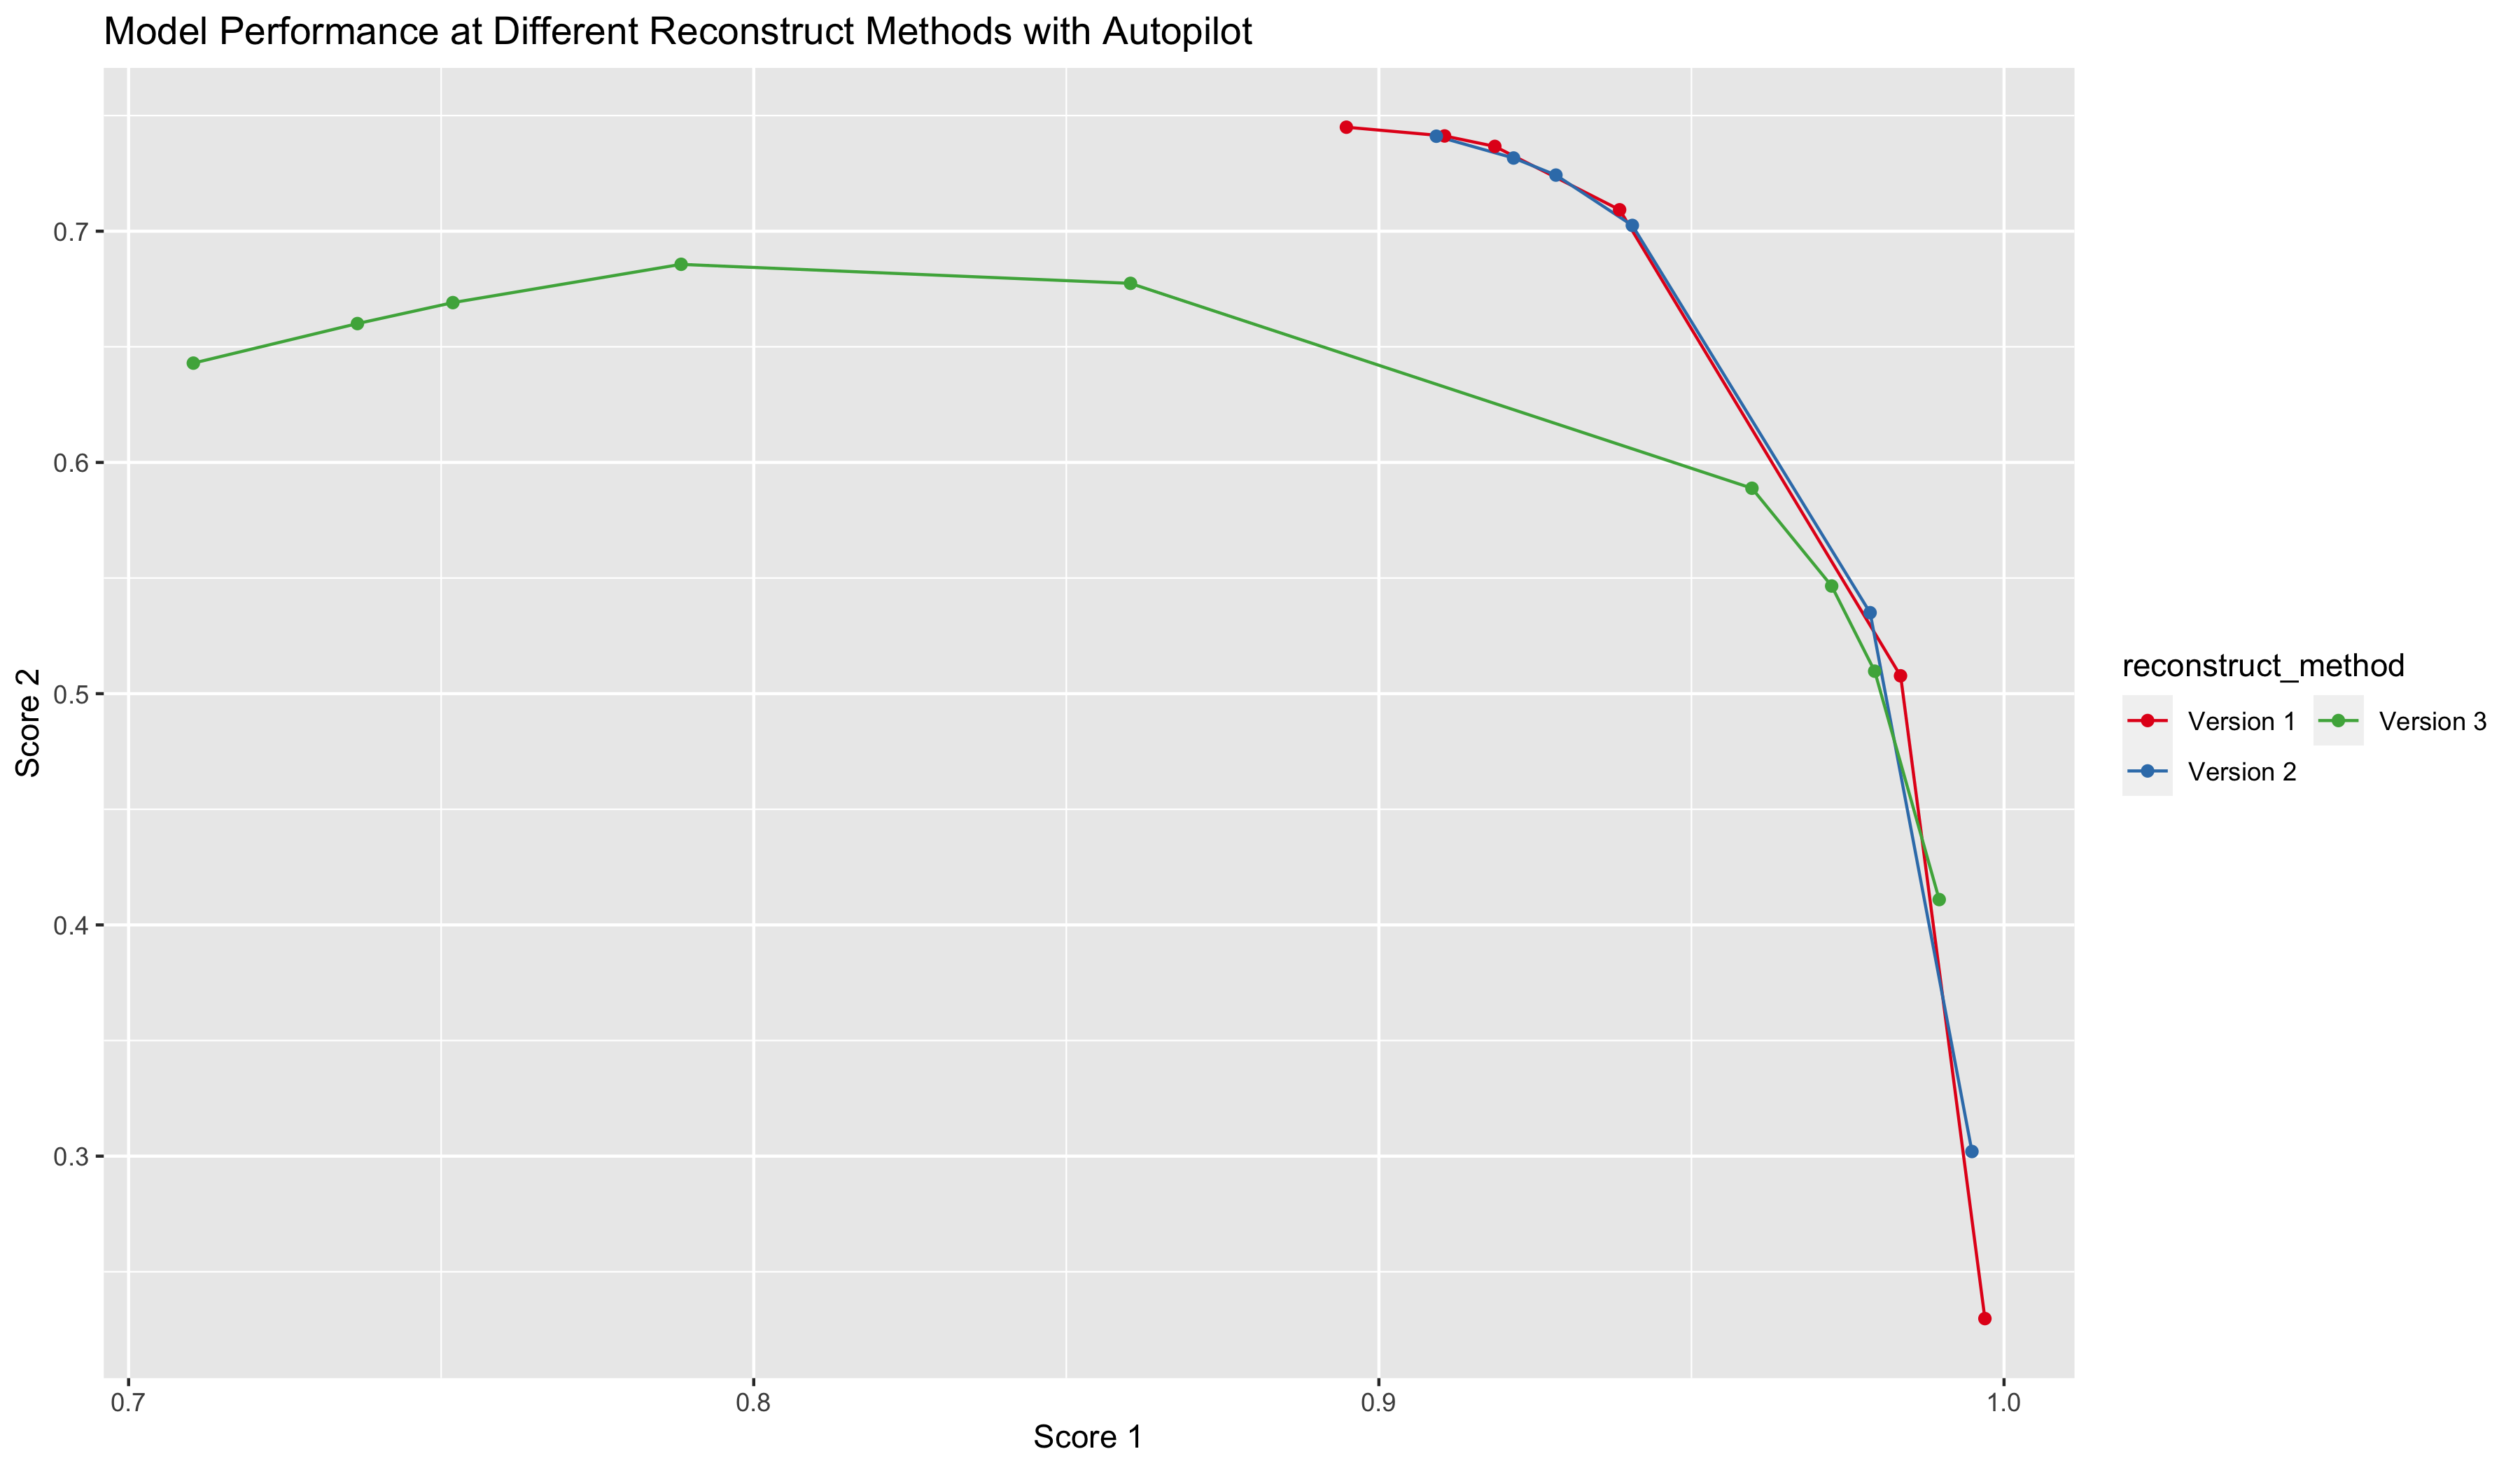
\includegraphics{images/ModelPerformanceatDifferentReconstructMethodswithAutopilot.png}
    \label{fig:fig1.11.1}
\end{figure}

\begin{table}[htbp]
  \begin{center}
    \caption{Configuration and Result of Different j-quantile for Predicting Maximum of Next 5min Window Using Autopilot}
    \label{tab:tab1.11.1}
    \begin{tabular}{l|l|*{4}{c}} \textbf{reconstruct method} & \textbf{j} &
      \textbf{score 1} & \textbf{score 1 weight} & \textbf{score 2} &
      \textbf{score 2 weight} \\
      \hline
      Version 1 & 0.001 & 0.9969 & 414249 & 0.2298 & 716235\\
      Version 1 & 0.010 & 0.9834 & 614705 & 0.5077 & 716235\\
      Version 1 & 0.050 & 0.9385 & 678510 & 0.7093 & 716235\\
      Version 1 & 0.070 & 0.9185 & 682062 & 0.7367 & 716235\\
      Version 1 & 0.080 & 0.9105 & 683368 & 0.7412 & 716235\\
      Version 1 & 0.100 & 0.8948 & 686723 & 0.7450 & 716235\\
      Version 2 & 0.001 & 0.9949 & 519172 & 0.3020 & 714840\\
      Version 2 & 0.010 & 0.9786 & 642181 & 0.5350 & 714840\\
      Version 2 & 0.050 & 0.9405 & 680123 & 0.7025 & 714840\\
      Version 2 & 0.070 & 0.9283 & 682283 & 0.7243 & 714840\\
      Version 2 & 0.080 & 0.9215 & 684080 & 0.7316 & 714840\\
      Version 2 & 0.100 & 0.9092 & 688740 & 0.7411 & 714840\\
      Version 3 & 0.0001 & 0.9896 & 556478 & 0.4110 & 716235\\
      Version 3 & 0.0003 & 0.9793 & 611494 & 0.5097 & 716235\\
      Version 3 & 0.0005 & 0.9724 & 623478 & 0.5465 & 716235\\
      Version 3 & 0.0010 & 0.9597 & 637230 & 0.5888 & 716235\\
      Version 3 & 0.0100 & 0.8603 & 694175 & 0.6774 & 716235\\
      Version 3 & 0.0500 & 0.7884 & 709186 & 0.6857 & 716235\\
      Version 3 & 0.0700 & 0.7519 & 711860 & 0.6691 & 716235\\
      Version 3 & 0.0800 & 0.7366 & 713910 & 0.6600 & 716235\\
      Version 3 & 0.1000 & 0.7104 & 716169 & 0.6429 & 716235\\
    \end{tabular}
  \end{center}
\end{table}

\begin{table}[htbp]
  \begin{center}
    \caption{Configuration and Result of Different half-life for Predicting Maximum of Next 5min Window Using Autopilot}
    \label{tab:tab1.11.2}
    \begin{tabular}{{l}|{l}|*{4}{c}} \textbf{reconstruct method} &
      \textbf{half-life} & \textbf{score 1} & \textbf{score 1 weight} &
      \textbf{score 2} & \textbf{score 2 weight} \\
      \hline
      Version 1 & 5m & 0.9219 & 671071 & 0.6973 & 716235\\
      Version 1 & 15m & 0.9532 & 651747 & 0.6357 & 716235\\
      Version 1 & 30m & 0.9704 & 640185 & 0.6089 & 716235\\
      Version 1 & 1h & 0.9778 & 0.629084 & 0.5746 & 716235\\
      Version 1 & 3h & 0.9821 & 623970 & 0.5447 & 716235\\
      Version 1 & 6h & 0.9830 & 619511 & 0.5267 & 716235\\
      Version 1 & 12h & 0.9834 & 614705 & 0.5077 & 716235\\
      Version 2 & 5m & 0.9197 & 676015 & 0.7027 & 714840\\
      Version 2 & 15m & 0.9517 & 665934 & 0.6592 & 714840\\
      Version 2 & 30m & 0.9641 & 661236 & 0.6328 & 714840\\
      Version 2 & 1h & 0.9712 & 657391 & 0.6081 & 714840\\
      Version 2 & 3h & 0.9763 & 652231 & 0.5742 & 714840\\
      Version 2 & 6h & 0.9776 & 647396 & 0.5534 & 714840\\
      Version 2 & 12h & 0.9786 & 642181 & 0.5350 & 714840\\
    \end{tabular}
  \end{center}
\end{table}

\begin{table}[htbp]
  \begin{center}
    \caption{Configuration and Result of Different Number of Breaks for Predicting Maximum of Next 5min Window Using Autopilot}
    \label{tab:tab1.11.3}
    \begin{tabular}{{l}|{l}|*{4}{c}} \textbf{reconstruct method} &
      \textbf{number of breaks} & \textbf{score 1} & \textbf{score 1 weight} &
      \textbf{score 2} & \textbf{score 2 weight} \\
      \hline
      Version 1 & 10 & 0.9834 & 614705 & 0.5077 & 716235\\
      Version 1 & 20 & 0.9803 & 647914 & 0.5348 & 716235\\
      Version 1 & 50 & 0.9774 & 676506 & 0.5512 & 716235\\
      Version 2 & 10 & 0.9786 & 642181 & 0.5350 & 714840\\
      Version 2 & 20 & 0.9741 & 664348 & 0.5620 & 714840\\
      Version 2 & 50 & 0.9708 & 678997 & 0.5780 & 714840\\
    \end{tabular}
  \end{center}
\end{table}

\begin{table}[htbp]
  \begin{center}
    \caption{Configuration and Result of Different Window Sizes for Predicting Maximum of Next Window Using Autopilot}
    \label{tab:tab1.11.4}
    \begin{tabular}{{l}|{l}|{l}|*{4}{c}} \textbf{reconstruct method} &
    \textbf{window size} & \textbf{half life} & \textbf{score 1} & \textbf{score
    1 weight} & \textbf{score 2} & \textbf{score 2 weight} \\
      \hline
      Version 1 & 1h & 20m & 0.8340 & 51820 & 0.5334 & 59548\\
      Version 1 & 1h & 1h & 0.8478 & 51220 & 0.5172 & 59548\\
      Version 1 & 1h & 4h & 0.8602 & 51231 & 0.5011 & 59548\\
      Version 1 & 1h & 12h & 0.8638 & 51766 & 0.4954 & 59548\\
      Version 1 & 1h & 24h & 0.8623 & 51561 & 0.4911 & 59548\\
      Version 1 & 1h & 48h & 0.8600 & 51491 & 0.4895 & 59548\\
      Version 1 & 3h & 1h & 0.6420 & 17069 & 0.4184 & 19762\\
      Version 1 & 3h & 3h & 0.6657 & 17033 & 0.4206 & 19762\\
      Version 1 & 3h & 12h & 0.6869 & 17255 & 0.4262 & 19762\\
      Version 1 & 3h & 36h & 0.6832 & 17158 & 0.4210 & 19762\\
      Version 1 & 3h & 72h & 0.6819 & 17173 & 0.4197 & 19762\\
      Version 1 & 3h & 144h & 0.6811 & 17177 & 0.4193 & 19762\\
      Version 2 & 1h & 20m & 0.7852 & 54120 & 0.5340 & 59349\\
      Version 2 & 1h & 1h & 0.8025 & 53432 & 0.5200 & 59349\\
      Version 2 & 1h & 4h & 0.8146 & 53728 & 0.5056 & 59349\\
      Version 2 & 1h & 12h & 0.8180 & 54190 & 0.5048 & 59349\\
      Version 2 & 1h & 24h & 0.8153 & 54058 & 0.5016 & 59349\\
      Version 2 & 1h & 48h & 0.8138 & 53792 & 0.5006 & 59349\\
      Version 2 & 3h & 1h & 0.5826 & 17788 & 0.4029 & 19667\\
      Version 2 & 3h & 3h & 0.6054 & 17796 & 0.4041 & 19667\\
      Version 2 & 3h & 12h & 0.6219 & 18034 & 0.4121 & 19667\\
      Version 2 & 3h & 36h & 0.6175 & 17946 & 0.4075 & 19667\\
      Version 2 & 3h & 72h & 0.6154 & 17902 & 0.4063 & 19667\\
      Version 2 & 3h & 144h & 0.6148 & 17904 & 0.4059 & 19667\\
    \end{tabular}
  \end{center}
\end{table}

\begin{table}[htbp]
  \begin{center}
    \caption{Configurations and Results of Different models for Predicting Maximum of Next Windows}
    \label{tab:tab1.11.5}
    \begin{tabular}{{l}|{l}|{l}|*{4}{c}} \textbf{model} & \textbf{cut off prob}
      & \textbf{window} & \textbf{score 1} & \textbf{score 1 weight} &
      \textbf{score 2} & \textbf{score 2 weight} \\
      \hline
      AR1 online(fixed) & 0.01 & 10m & 0.9643 & 334769 & 0.5805 & 357435\\
      AR1 online(fixed) & 0.01 & 15m & 0.9609 & 217810 & 0.5295 & 238038\\
      AR1 online(fixed) & 0.01 & 30m & 0.9542 & 101981 & 0.4499 & 118942\\
      AR1 online(fixed) & 0.01 & 01h & 0.9504 & 047518 & 0.3873 & 059249\\
      AR1 online(fixed) & 0.01 & 03h & 0.9287 & 012797 & 0.2439 & 019661\\
      AR1 online(fixed) & 0.03 & 10m & 0.9467 & 339404 & 0.6279 & 357435\\
      AR1 online(fixed) & 0.03 & 15m & 0.9463 & 223975 & 0.5867 & 238038\\
      AR1 online(fixed) & 0.03 & 30m & 0.9372 & 108094 & 0.5123 & 118942\\
      AR1 online(fixed) & 0.03 & 01h & 0.9319 & 050406 & 0.4498 & 059249\\
      AR1 online(fixed) & 0.03 & 03h & 0.9101 & 014947 & 0.3134 & 019661\\
      Autopilot & 0.01 & 10m & 0.9555 & 309666 & 0.5366 & 357899\\
      Autopilot & 0.01 & 15m & 0.9433 & 205504 & 0.5280 & 238514\\
      Autopilot & 0.01 & 30m & 0.9081 & 111959 & 0.5142 & 119133\\
      Autopilot & 0.01 & 01h & 0.8492 & 051011 & 0.5014 & 059443\\
      Autopilot & 0.01 & 03h & 0.6809 & 017156 & 0.4245 & 019662\\
      Autopilot & 0.03 & 10m & 0.9031 & 334336 & 0.6493 & 357899\\
      Autopilot & 0.03 & 15m & 0.8754 & 223237 & 0.6379 & 238514\\
      Autopilot & 0.03 & 30m & 0.7987 & 111959 & 0.6001 & 119133\\
      Autopilot & 0.03 & 01h & 0.6744 & 056028 & 0.5312 & 059443\\
      Autopilot & 0.03 & 03h & 0.4237 & 018608 & 0.3370 & 019662\\
    \end{tabular}
  \end{center}
\end{table}

\section{Prediction of Background Jobs}
\subsection{Main Motivation for the problem}

\begin{flushleft}
In the foreground part, the time series models do the prediction of the amount
of available resource that can be scheduled in the next period of time, with the
constraint for the overall survival rate. However, we do not know for sure how
long a specific job will last in the machine. Therefore, we are aiming to
predict the distribution of job's duration times, as a discrete probability
vector: $(p_1, p_2, ..., p_m)$, which can be used later with the models for the
foreground part, to decide which job should be assigned to which machine.
\end{flushleft}

\begin{flushleft}
The methodology in this part can be decomposed into the following parts:
\begin{itemize}
    \item Discretization of the job duration times.
    \item Clustering of jobs
    \item Building probability vector within each cluster
    \item Diagnosis and Updating of the probability vectors
\end{itemize}
\end{flushleft}

\subsection{Discretization}

\begin{flushleft}
The reason that we need to do the discretization for job's duration time is that
for each unique value of job's duration time, we need to correspond with a
separate model in the foreground part. Since in practice we can only have
finitely many models in each part, we need to discretize the duration times into
finitely many distinct bins.

The first step for do a visualization of the unconditional job duration times,
and decide the number and placement of our bins.

Based on this histogram Fig \ref{fig:fig2.2.1}, a reasonable bin vector will
be:\newline $(0,1,2,6,10,14,18,22,26,30,50,80,205)$, which covers the full range
of job duration in this case, and places bins with smaller widths for region
with greater density. Therefore, the discretized values of job duration will
be\newline $(1,2,6,10,14,18,22,26,30,50,80,205)$ depending on which bin that job
duration is in.
\end{flushleft}

\subsection{Clustering of jobs}

\begin{flushleft}
To make the probability vector a more accurate approximation for job's
duration's distribution, jobs are assigned to different clusters. The clustering
algorithms use job's features: priority, scheduling class, requested CPU,
requested RAM and requested local disk space. There are two options available
for the clustering algorithm.
\end{flushleft}

\subsubsection{Tree Method}

\begin{flushleft}
Using the training set, a \textbf{survival tree} or a \textbf{regression tree}
that aims to predict the job's duration is fitted, and each terminal node will
be regarded as a cluster for jobs. The survival tree treats each observation of
the job's duration as a realization from a specific exponential distribution,
with each terminal node in the tree represents a different type of exponential
distribution, and seeks to maximize a likelihood criterion. The regression tree
just treats each duration as a usual continuous numerical variable and seeks to
minimize the sum of squares. The number of clusters will be the number of
terminal nodes in the tree, so it does not need to be specified beforehand.
\end{flushleft}

\begin{flushleft}
\textbf{minsize}: Minsize used when the tree method is selected for the
clustering. It specifies the minimum number of observations in each terminal
node of the tree. To make sure later the probability vector in each cluster is
estimated accurately, it is necessary to make sure that there are enough
observations in each cluster.
\end{flushleft}

\subsubsection{Gaussian Mixture Model Method}

\begin{flushleft}
Different from the tree method above, the GMM method does the clustering without
looking at the response variable duration time. This method simply treats the
features of each job are multivariate normally distributed, and models the whole
data-set as a mixture of normal distributions. To use this algorithm, it is
necessary to know the number of clusters in the data set. So without this
information, the algorithm will automatically try for a bunch of numbers and
select the one with the optimal BIC value.
\end{flushleft}

\begin{flushleft}
\textbf{upperlimBIC}: Upper Limit BIC used when the GMM method is selected. It
specifies the maximum number of cluster that the algorithm will try when it is
selecting the number of clusters in the model.
\end{flushleft}

\subsection{Building probability vector}

\begin{flushleft}
After obtaining a model for the clustering, and a clustered training set, a
probability vector can be estimated in each cluster by looking at the empirical
distribution(histogram). For example, if we discretized the job duration time
into m discrete values, and found out that there are k clusters after the
clustering, then we are looking for a list of k vectors, each with m components,
i.e.: $\{(p_{i1}, p_{i2}, ..., p_{im}) : i \in (1,...,k)\}$. The value of
$p_{ij}$ can be interpreted as the probability that a job in cluster i, has
duration time $t_j$ (the j-th distinct duration time after discretization).
\end{flushleft}

\subsection{Diagnosis and Updating}

\begin{flushleft}
To test the accuracy of probability vectors we obtained from training set, we
use the probability vectors obtained from the testing set, by measuring the
average squared error weighted by the number of observations in each labeled
testing set. (For this measure to make sense, we need the number of observations
in the unconditional testing set to be large enough, but not necessary for each
labeled testing set, as they are already weighted). For example, denote the
number of observations in the (unconditional) testing set as $T$, and the number
of observations in cluster i in the testing set as $T_i$, and let $\{(q_{i1},
q_{i2}, ..., q_{im}) : i \in (1,...,k)\}$ be the list of probability vectors
obtained from the testing set, then our measure of discrepancy will be:
\end{flushleft}

\begin{flushleft}
\begin{equation}
\centering
        \sum_{i = 1} ^{k} \frac{T_i}{T} \sum_{j = 1}^{m} \frac{(q_{ij} - p_{ij})^2}{m}
\end{equation}
\end{flushleft}

\begin{flushleft}
When this value is too large, it might be that users have now changed their
usual behavior, and we need to gradually adopt their new behavior by updating
our probability vector. It could be done by randomly dropping observations from
the unconditional training set, and replace these observations by the testing
set we used and recompute the probability vector.
\end{flushleft}

\subsection{Appendix}

\subsubsection{Discretization}

\begin{figure}[htbp]
\caption{Unconditional Histogram of Job Duration}
\centering
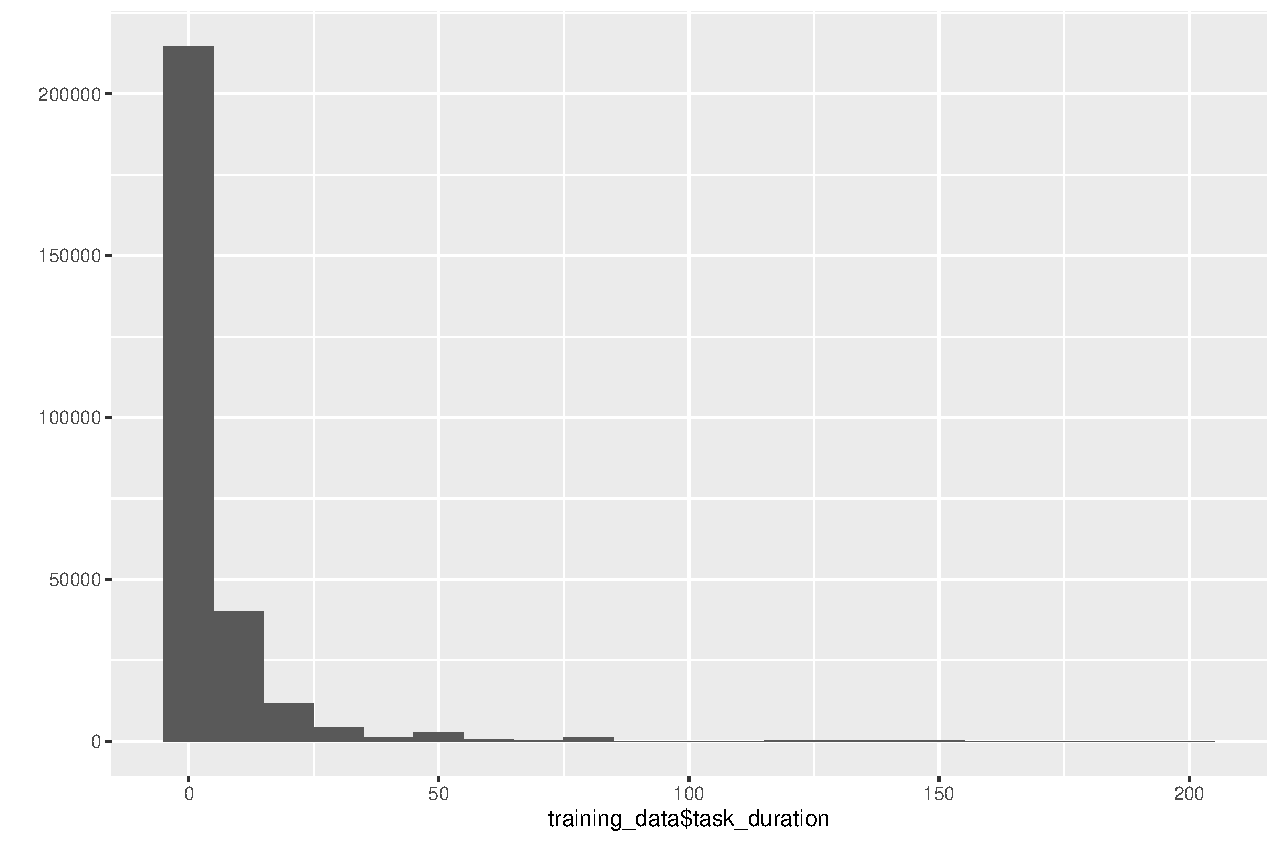
\includegraphics[width = 0.8\textwidth]{uncondional_hist}
\label{fig:fig2.2.1}
\end{figure}

\section{Combining Predictions of Two Parts}
\subsection{Overview of Current method}
\begin{flushleft}
Our current method of combining foreground jobs model and background jobs model
can be summarized as following:

\begin{enumerate}[Step 1:]
    \item Given a job, we use the clustering model from the background part to
    identify which cluster it is in. Let its requested CPU be $R$.
    \item Using the probability vector of this cluster from background part, we
    know the probability of this job finishing at different times. Let's suppose
    that the probability vector is $P = (p_{1}, ..., p_{m})$
    \item There will be also m models running on the foreground part, and each
    of them will have a aggregation time correspond to a component of the
    discretized job duration times. Each of these models will give a one-step
    forward prediction for the available resource on the machine. Call this
    vector of one step predictions as $(r_1, ... , r_m)$.
    \item Notice that $r_i$ can be interpreted as the amount of available
    resource given that time T equals $t_i$. So the expected available resource
    for this job is computed as $U = \sum_{i=1}^{m} p_i r_i$.
    \item For the j-th machine, we can compute the probability that the i-th job
    can be finished, by summing over the components in the probability vector
    such that $r_j \geq R_i$. If this sum is greater than the specified
    threshold (a default value is $\sqrt{99}$ percent), we call this machine is
    plausible for the job. 
    \item For the j-th machine, compute the cost $D_j$ as:$U_j - R$ if $R \leq
    U_j$, and $\infty$ otherwise. Then among all the plausible machines, we will
    choose to allocate a job to the machine with minimum cost.
\end{enumerate}

\textbf{Order of Scheduling Jobs}: Since scheduling multiple jobs on multiple
machines with some capacities is a multi-dimensional knapsack problem which is
an NP hard problem. A simple approximation algorithm we proposed is to order the
jobs by their requested CPU and consecutively scheduled (following Step 4, Step
5 and Step 6).

\textbf{Killing Jobs}: Sometimes outliers or irregular fluctuations may occur
and the foreground CPU resource may interfere with background scheduled jobs. In
this case, we need to at least free up the CPU resource scheduled subtracted by
CPU resource actually available, denoted by $C$.

In order to find the suitable jobs to kill to minimize the number of jobs being
killed while also minimizing CPU utilization lost, a two-step dynamic
programming algorithm is implemented: First, order the current scheduled jobs by
their requested CPU in descending order, then by consecutively removing the jobs
in order, we can find the minimum number of jobs that needs to be killed in
order to accommodate the spike in foreground CPU resource. Second, we
consecutively select the minimum number of jobs to kill with minimum resource
occupied of $C$ at this time of while minimizing the loss of CPU resource as the
result of killing such selected jobs, that is, the sum of product of CPU
resource requested and the amount of time the job has been running. A dynamic
programming algorithm in the second step would significantly reduce the run
time.

It is also noticeable that the running time of the above is approximately
$O(n^k)$ where $n$ is the number of jobs active at any timestamp, $k$ is an
integer greater than $0$ as the number of jobs that needs to be killed. Another
alternative is simply order the jobs by their requested CPU in descending order
and select jobs from top of the list to kill. This approach significantly reduce
the running time and does not have any impact on survival rate since the number
of jobs being killed is exactly the same as dynamic programming algorithm
described above, but the utilization rate will be lower since the whole purpose
of the dynamic programming algorithm is to find smallest job to kill.

\textbf{Randomized Simulation}: There are two parts of the simulations that are
random; the arrival time of the jobs are uniformly assigned across all
simulation time length and the machine selected. In order to generate more
stable results, each simulation is repeated at least 10 times and averaged as
the final performance.
\end{flushleft}

\subsection{Simulation Study}

\begin{flushleft}
The purpose of these simulations is to deal with the case of how to allocate
each job into the optimal machine (we want it to survive, but not to waste so
much resource). We used the google data set for jobs, and the Microsoft data set
for foreground predictions.
\end{flushleft}

\begin{flushleft}
The foreground setting of simulation is to use simple AR1 model with offline
training strategy, with training size of 3000 data points and the length of
simulation is 100 unit time (500 minutes). The background setting of simulation
is to use ANOVA tree model on clustering and 5000 jobs as training set.
\end{flushleft}

\subsubsection{Arrival Rate}

\begin{flushleft}
Arrival rate refers to the number of jobs arrivals per unit of time. If all the
jobs can be ideally scheduled onto the machines, the arrival rate is considered
to be \textbf{sparse}, and if the jobs are competing for resources and a
significant proportion of jobs cannot be scheduled eventually, then the arrival
rate is considered to be \textbf{dense}.

\textbf{Load of Jobs}: The load of jobs is an indicator of how dense the arrival
rate is for fixed choices of machines. It is simply the sum of CPU resource
requested by all jobs times their running time divided by the resource available
across all machines summed at all simulation time. When the load is close to
$1$, a small proportion of the jobs may eventually fail to be scheduled, and
when the load is much greater than $1$, the jobs are competing for resources and
all machines can be presumed to be fully occupied at all time.

Table \ref{tab:tab3.2.1} shows that the performance of survival rate is not
affected by the arrival rate or the load, the utilization becomes better as
arrival rate increases because more choices of jobs becomes available at higher
rates, and the algorithm may have better selections.

Another method of changing the arrival rate is to increase the simulation
length, Table \ref{tab:tab3.2.2} shows that fixing the number of background jobs
to be $5000$ as simulation length increases, the utilization decreases but there
is not significant change in survival rate.
\end{flushleft}

\subsubsection{Cut off Probability}

\begin{flushleft}
In the above experiments, we have used cut off probability 
\end{flushleft}

\subsubsection{Models for Background Jobs}

\begin{flushleft}
As described in the Tree Methods and GMM Methods in the previous section, we aim
to compare the performance of simulation results using the different models for
clustering background jobs. Evidently different tree methods yields similar tree
structure and Table \ref{tab:tab3.2.3} suggests that the two tree methods have
similar performance in both survival rate and utilization rate.
\end{flushleft}

\subsubsection{Models for Foreground Jobs}
Since using different models yields different prediction upper bounds, which are
used to determine the available resource at each time window.

\subsection{Appendix}

\subsubsection{Simulation Study}

\begin{table}[htbp]
  \begin{center}
    \caption{Combined Simulation of AR1 Model and ANOVA tree with Different Number of Jobs}
    \label{tab:tab3.2.1}
    \begin{tabular}{{l}|*{5}{c}} \textbf{job num} & \textbf{finished
      utilization} & \textbf{survival rate} & \textbf{load} & \textbf{unfinished
      rate} & \textbf{unscheduled rate} \\
      \hline
      1000 & 0.1185 & 0.9966 & 0.8077 & 0.0070 & 0.4038\\
      2000 & 0.1808 & 0.9956 & 1.5285 & 0.0024 & 0.5262\\
      3000 & 0.1877 & 0.9937 & 1.8106 & 0.0017 & 0.6019\\
      5000 & 0.2950 & 0.9965 & 2.7880 & 0.0015 & 0.6405\\
    \end{tabular}
  \end{center}
\end{table}

\begin{table}[htbp]
  \begin{center}
    \caption{Combined Simulation of AR1 Model and ANOVA tree with Different Length of Simulation}
    \label{tab:tab3.2.2}
    \begin{tabular}{{l}|*{5}{c}} \textbf{sim length} & \textbf{finished
      utilization} & \textbf{survival rate} & \textbf{load} & \textbf{unfinished
      rate} & \textbf{unscheduled rate} \\
      \hline
      100 & 0.2950 & 0.9965 & 2.7880 & 0.0015 & 0.6405\\
      200 & 0.2490 & 0.9953 & 1.3927 & 0.0016 & 0.5003\\
      500 & 0.2465 & 0.9923 & 0.5649 & 0.0009 & 0.1608\\
      1000 & 0.1645 & 0.9926 & 0.2828 & 0.0005 & 0.1435\\
      1500 & 0.0938 & 0.9965 & 0.1857 & 0.0003 & 0.1897\\
    \end{tabular}
  \end{center}
\end{table}

\begin{table}[htbp]
  \begin{center}
    \caption{Combined Simulation of AR1 Model and Different Background Models}
    \label{tab:tab3.2.3}
    \begin{tabular}{{l}|*{5}{c}} \textbf{background model} & \textbf{finished
      utilization} & \textbf{survival rate} & \textbf{load} & \textbf{unfinished
      rate} & \textbf{unscheduled rate} \\
      \hline
      anova tree & 0.2950 & 0.9965 & 2.7880 & 0.0015 & 0.6405\\
      survival tree & 0.2993 & 0.9956 & 2.5562 & 0.0011 & 0.5568\\
    \end{tabular}
  \end{center}
\end{table}

\begin{longtable}[htbp]{{l}|{l}|{l}|*{5}{c}}
    \caption{Combined Simulation of AR1 and Autopilot with Different Length of Simulation}
    \label{tab:tab3.2.4} \\
    \textbf{model} & \textbf{sim length} & \textbf{alpha} & \textbf{finished
    utilization} & \textbf{survival rate} & \textbf{load} & \textbf{unfinished
    rate} & \textbf{unscheduled rate} \\
    \hline
    Autopilot & 1000 & 0.005 & 0.1932 & 0.9947 & 0.2858 & 0.0006 & 0.1594\\
    Autopilot & 1000 & 0.01 & 0.2055 & 0.9927 & 0.2858 & 0.0006 & 0.0928\\
    Autopilot & 1000 & 0.02 & 0.2137 & 0.9889 & 0.2858 & 0.0006 & 0.0778\\
    Autopilot & 1000 & 0.05 & 0.1898 & 0.9743 & 0.2858 & 0.0006 & 0.0307\\
    Autopilot & 1500 & 0.005 & 0.1390 & 0.9945 & 0.1681 & 0.0007 & 0.0227\\
    Autopilot & 1500 & 0.01 & 0.1358 & 0.9914 & 0.1681 & 0.0005 & 0.0221\\
    Autopilot & 1500 & 0.02 & 0.1274 & 0.9886 & 0.1681 & 0.0006 & 0.0221\\
    Autopilot & 1500 & 0.05 & 0.1238 & 0.9852 & 0.1681 & 0.0005 & 0.0221\\
    Autopilot & 2000 & 0.005 & 0.1187 & 0.9948 & 0.1391 & 0.0003 & 0.0382\\
    Autopilot & 2000 & 0.01 & 0.1168 & 0.9914 & 0.1391 & 0.0003 & 0.0148\\
    Autopilot & 2000 & 0.02 & 0.1026 & 0.9816 & 0.1391 & 0.0003 & 0.0148\\
    Autopilot & 2000 & 0.05 & 0.0916 & 0.9733 & 0.1391 & 0.0002 & 0.0148\\
    AR1 offline & 1000 & 0.005 & 0.1190 & 0.9839 & 0.2858 & 0.0006 & 0.1902\\
    AR1 offline & 1000 & 0.01 & 0.1370 & 0.9846 & 0.2858 & 0.0006 & 0.1546\\
    AR1 offline & 1000 & 0.02 & 0.1627 & 0.9844 & 0.2858 & 0.0006 & 0.0833\\
    AR1 offline & 1000 & 0.05 & 0.1883 & 0.9862 & 0.2858 & 0.0007 & 0.0466\\
    AR1 offline & 1500 & 0.005 & 0.1213 & 0.9947 & 0.1681 & 0.0006 & 0.0438\\
    AR1 offline & 1500 & 0.01 & 0.1290 & 0.9946 & 0.1681 & 0.0006 & 0.0309\\
    AR1 offline & 1500 & 0.02 & 0.1349 & 0.9940 & 0.1681 & 0.0006 & 0.0249\\
    AR1 offline & 1500 & 0.05 & 0.1372 & 0.9936 & 0.1681 & 0.0006 & 0.0225\\
    AR1 online & 1000 & 0.005 & 0.1195 & 0.9962 & 0.2858 & 0.0005 & 0.1908\\
    AR1 online & 1000 & 0.01 & 0.1424 & 0.9973 & 0.2858 & 0.0005 & 0.1409\\
    AR1 online & 1000 & 0.02 & 0.1712 & 0.9948 & 0.2858 & 0.0006 & 0.0884\\
    AR1 online & 1000 & 0.05 & 0.2013 & 0.9928 & 0.2858 & 0.0006 & 0.0490\\
    AR1 online & 1000 & 0.06 & 0.2028 & 0.9913 & 0.2858 & 0.0007 & 0.0474\\
    AR1 online & 1000 & 0.07 & 0.2078 & 0.9905 & 0.2858 & 0.0007 & 0.0415\\
    AR1 online & 1000 & 0.08 & 0.2106 & 0.9916 & 0.2858 & 0.0006 & 0.0433\\
    AR1 online & 1000 & 0.09 & 0.2091 & 0.9908 & 0.2858 & 0.0006 & 0.0425\\
    AR1 online & 1500 & 0.005 & 0.1174 & 0.9975 & 0.1681 & 0.0005 & 0.0483\\
    AR1 online & 1500 & 0.01 & 0.1301 & 0.9971 & 0.1681 & 0.0006 & 0.0338\\
    AR1 online & 1500 & 0.02 & 0.1358 & 0.9957 & 0.1681 & 0.0006 & 0.0277\\
    AR1 online & 1500 & 0.05 & 0.1397 & 0.9942 & 0.1681 & 0.0006 & 0.0230\\
    AR1 online & 1500 & 0.06 & 0.1413 & 0.9942 & 0.1681 & 0.0006 & 0.0227\\
    AR1 online & 1500 & 0.07 & 0.1404 & 0.9938 & 0.1681 & 0.0006 & 0.0225\\
    AR1 online & 1500 & 0.08 & 0.1408 & 0.9933 & 0.1681 & 0.0006 & 0.0223\\
    AR1 online & 1500 & 0.09 & 0.1387 & 0.9927 & 0.1681 & 0.0006 & 0.0222\\
    AR1 online & 2000 & 0.005 & 0.0860 & 0.9968 & 0.1391 & 0.0003 & 0.0901\\
    AR1 online & 2000 & 0.01 & 0.0966 & 0.9971 & 0.1391 & 0.0003 & 0.0607\\
    AR1 online & 2000 & 0.02 & 0.1075 & 0.9973 & 0.1391 & 0.0003 & 0.0436\\
    AR1 online & 2000 & 0.05 & 0.1167 & 0.9958 & 0.1391 & 0.0003 & 0.0188\\
    AR1 online & 2000 & 0.06 & 0.1186 & 0.9952 & 0.1391 & 0.0003 & 0.0166\\
    AR1 online & 2000 & 0.07 & 0.1186 & 0.9955 & 0.1391 & 0.0003 & 0.0161\\
    AR1 online & 2000 & 0.08 & 0.1191 & 0.9950 & 0.1391 & 0.0003 & 0.0161\\
    AR1 online & 2000 & 0.09 & 0.1193 & 0.9947 & 0.1391 & 0.0003 & 0.0160\\
\end{longtable}
  
\begin{table}[htbp]
  \begin{center}
    \caption{Combined Simulation of Different Foreground Models and ANOVA tree with 500 Simulation Length}
    \label{tab:tab3.2.5}
    \begin{tabular}{{l}|{l}|*{5}{c}} \textbf{model} & \textbf{cut off prob} &
      \textbf{finished utilization} & \textbf{survival rate} & \textbf{load} &
      \textbf{unfinished rate} & \textbf{unscheduled rate} \\
      \hline
      AR1 online & 0.005 & 0.1877 & 0.9970 & 0.5776 & 0.0007 & 0.3005\\
      AR1 online & 0.010 & 0.2173 & 0.9974 & 0.5776 & 0.0007 & 0.2588\\
      AR1 online & 0.020 & 0.2519 & 0.9955 & 0.5776 & 0.0009 & 0.1800\\
      AR1 online & 0.050 & 0.3005 & 0.9893 & 0.5776 & 0.0010 & 0.1272\\
      AR1 online & 0.060 & 0.3135 & 0.9894 & 0.5776 & 0.0015 & 0.1292\\
      AR1 online & 0.070 & 0.3204 & 0.9880 & 0.5776 & 0.0011 & 0.1277\\
      AR1 online & 0.080 & 0.3195 & 0.9882 & 0.5776 & 0.0010 & 0.0986\\
      AR1 online & 0.090 & 0.3197 & 0.9878 & 0.5776 & 0.0011 & 0.1163\\
      VAR1 online & 0.005 & 0.2313 & 0.9912 & 0.5776 & 0.0009 & 0.2258\\
      VAR1 online & 0.010 & 0.2726 & 0.9944 & 0.5776 & 0.0010 & 0.1568\\
      VAR1 online & 0.020 & 0.3052 & 0.9931 & 0.5776 & 0.0010 & 0.1281\\
      VAR1 online & 0.050 & 0.3423 & 0.9910 & 0.5776 & 0.0011 & 0.0960\\
      VAR1 online & 0.060 & 0.3402 & 0.9900 & 0.5776 & 0.0011 & 0.0881\\
      VAR1 online & 0.070 & 0.3486 & 0.9899 & 0.5776 & 0.0011 & 0.0847\\
      VAR1 online & 0.080 & 0.3405 & 0.9873 & 0.5776 & 0.0011 & 0.0778\\
      VAR1 online & 0.090 & 0.3380 & 0.9871 & 0.5776 & 0.0011 & 0.0774\\
      NN online & 0.005 & 0.0000 & 0.0000 & 0.5776 & 0.0000 & 0.0000\\
      NN online & 0.010 & 0.0000 & 0.0000 & 0.5776 & 0.0000 & 0.0000\\
      NN online & 0.020 & 0.0000 & 0.0000 & 0.5776 & 0.0000 & 0.0000\\
      NN online & 0.050 & 0.0000 & 0.0000 & 0.5776 & 0.0000 & 0.0000\\
      Autopilot & 0.005 & 0.2998 & 0.9938 & 0.5776 & 0.0000 & 0.0000\\
      Autopilot & 0.010 & 0.3301 & 0.9905 & 0.5776 & 0.0011 & 0.2254\\
      Autopilot & 0.020 & 0.3410 & 0.9873 & 0.5776 & 0.0011 & 0.1368\\
      Autopilot & 0.050 & 0.3330 & 0.9736 & 0.5776 & 0.0011 & 0.0980\\
    \end{tabular}
  \end{center}
\end{table}

\begin{figure}[htbp]
\caption{Histogram of percent performance}
\centering
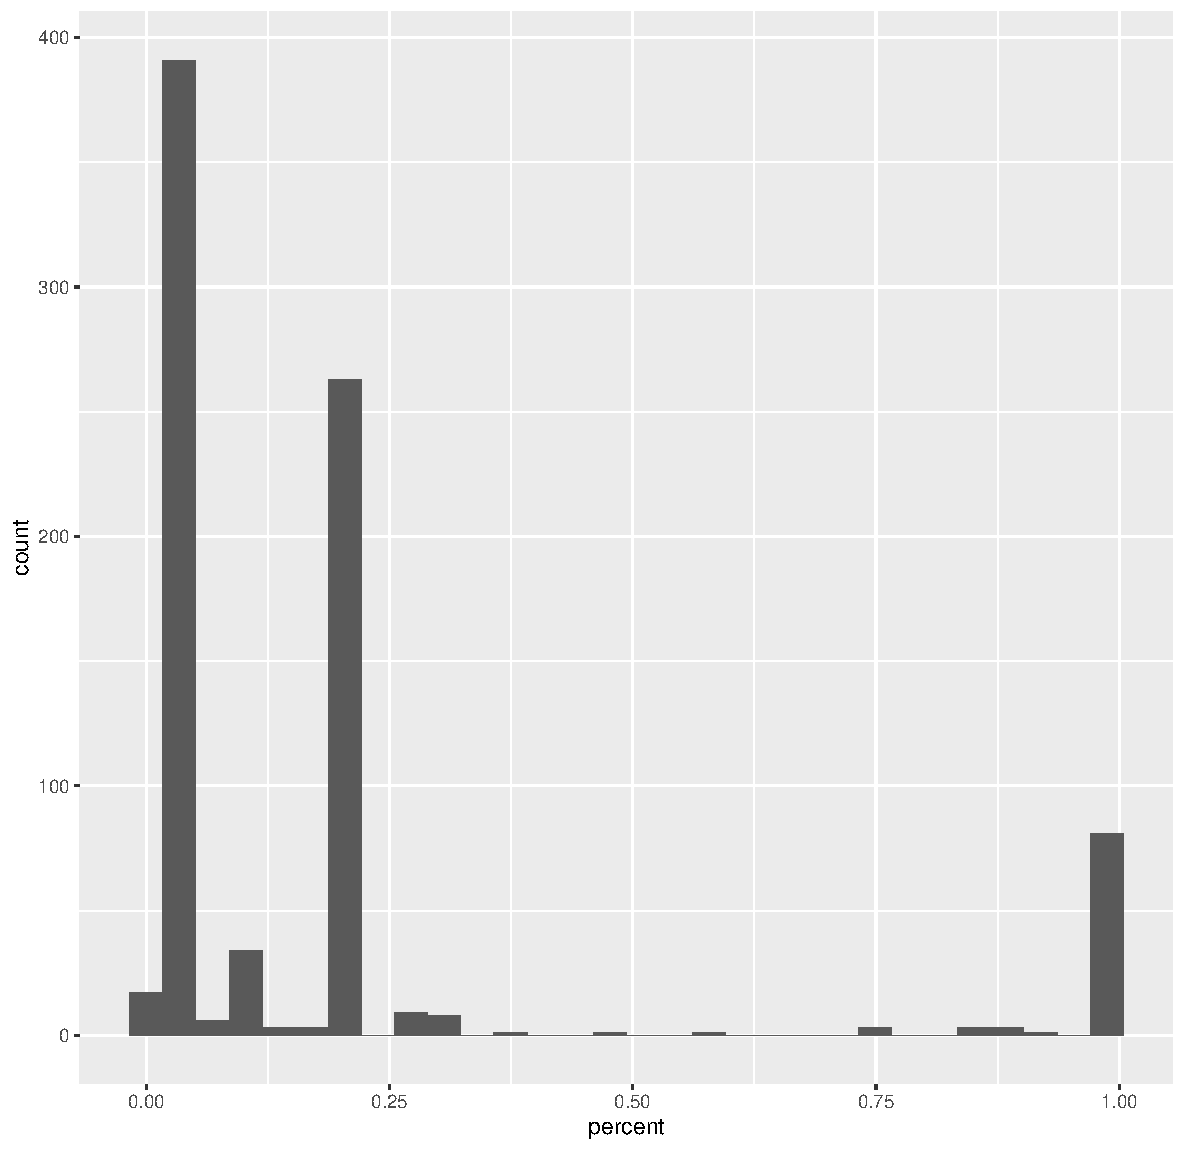
\includegraphics[width = 0.8\textwidth]{sur_tree}
\end{figure}

\end{document}
